\documentclass[11pt,a4paper]{book}
\usepackage[utf8]{inputenc}
\usepackage[margin=1in]{geometry}
\usepackage{amsmath,amssymb,amsthm}
\usepackage{graphicx}
\usepackage{tikz}
\usepackage{pgfplots}
\pgfplotsset{compat=1.17}
\usepackage{xcolor}
\usepackage{tcolorbox}
\usepackage{enumitem}
\usepackage{float}
\usepackage{hyperref}
\pgfplotsset{compat=1.17}
\usepackage{array}
\usepackage{booktabs}
\tcbuselibrary{breakable}
\usepackage{amsthm}
\usetikzlibrary{calc}


% Custom environments
\newtheorem{theorem}{Theorem}[section]
\newtheorem{lemma}[theorem]{Lemma}
\newtheorem{proposition}[theorem]{Proposition}
\theoremstyle{definition}
\newtheorem{definition}{Definition}[section]
\newtheorem{example}{Example}[section]
\theoremstyle{remark}
\newtheorem{remark}{Remark}[section]
\newtheorem{intuition}{Intuition}[section]

% Custom colored boxes
\newtcolorbox{keyidea}{
  colback=blue!5!white,
  colframe=blue!75!black,
  fonttitle=\bfseries,
  title=\large Key Idea,
  breakable,
  boxsep=4pt,
  top=4pt,
  bottom=4pt
}

\newtcolorbox{geometricintuition}{
  colback=green!5!white,
  colframe=green!75!black,
  fonttitle=\bfseries,
  title=\large Geometric Intuition,
  breakable,
  boxsep=4pt,
  top=4pt,
  bottom=4pt
}

\newtcolorbox{mentalmodel}{
  colback=orange!5!white,
  colframe=orange!75!black,
  fonttitle=\bfseries,
  title=\large Mental Model,
  breakable,
  boxsep=4pt,
  top=4pt,
  bottom=4pt
}

\newtcolorbox{importantbox}{
  colback=red!5!white,
  colframe=red!75!black,
  fonttitle=\bfseries,
  title=\large Important!,
  breakable,
  boxsep=4pt,
  top=4pt,
  bottom=4pt
}
% Custom environments
\newtheorem{corollary}[theorem]{Corollary}
\theoremstyle{definition}
\theoremstyle{remark}
\newtheorem{note}{Note}[section]


\newtcolorbox{geometrybox}{
  colback=green!5!white,
  colframe=green!75!black,
  fonttitle=\bfseries,
  title=\large Geometric Intuition,
  breakable,
  boxsep=4pt,
  top=4pt,
  bottom=4pt
}

\newtcolorbox{gatepoint}{
  colback=purple!5!white,
  colframe=purple!75!black,
  fonttitle=\bfseries,
  title=\large GATE Point,
  breakable,
  boxsep=4pt,
  top=4pt,
  bottom=4pt
}
\makeatletter
\renewenvironment{example}[1][]{%
  \refstepcounter{example}%
  \par\medskip
  \noindent\textbf{Example \theexample}%
  \if\relax\detokenize{#1}\relax
  \else\space\textbf{(#1)}%
  \fi
  \par\smallskip
}{%
  \par\medskip
}
\makeatother

\makeatletter
\renewenvironment{theorem}[1][]{%
  \refstepcounter{theorem}%
  \par\medskip
  \noindent\textbf{Theorem \thetheorem}%
  \if\relax\detokenize{#1}\relax
  \else\space\textbf{(#1)}%
  \fi
  \par\smallskip
}{%
  \par\medskip
}
\makeatother
\makeatletter
\renewenvironment{definition}[1][]{%
  \refstepcounter{definition}%
  \par\medskip
  \noindent\textbf{Definition \thedefinition}%
  \if\relax\detokenize{#1}\relax
  \else\space\textbf{(#1)}%
  \fi
  \par\smallskip
}{%
  \par\medskip
}
\makeatother


\title{\textbf{Machine Learning Notes} \\ 
\large{Understanding the Foundation of Machine Learning}}
\date{}

\begin{document}

\maketitle
\tableofcontents

\chapter{Simple Linear Regression: The Foundation Stone}

\section{What Are We Trying to Do? The Big Picture}

\begin{mentalmodel}
Imagine you're a detective looking at clues. You notice that whenever the temperature goes up by 10 degrees, ice cream sales increase by \$1000. You've discovered a \textbf{relationship}!

Machine learning is about finding these relationships automatically from data. Simple linear regression is the most basic form - finding straight-line relationships between two variables.
\end{mentalmodel}

\subsection{A Real-World Scenario}

Let's start with something concrete. You're helping a friend who sells houses. Over the years, you've noticed:

\begin{itemize}
    \item Small houses (1000 sq ft) sell for around \$200,000
    \item Medium houses (1500 sq ft) sell for around \$300,000
    \item Large houses (2000 sq ft) sell for around \$400,000
\end{itemize}

Now your friend asks: "I have a 1750 sq ft house. What should I price it at?"

Your brain naturally thinks: "Well, it's between 1500 and 2000, so probably around \$350,000..."

\textbf{Congratulations! You just did linear regression in your head!}

\subsection{The Three Fundamental Questions}

Every machine learning problem asks three questions:

\begin{enumerate}
    \item \textbf{What is my model?} (How do I represent the relationship?)
    \item \textbf{What does "best" mean?} (How do I measure if my model is good?)
    \item \textbf{How do I find the best model?} (What's the algorithm?)
\end{enumerate}

Let's answer these for simple linear regression.

\section{Question 1: What Is the Model?}

\subsection{The Straight Line - Our Model}

\begin{definition}[Simple Linear Regression Model]
We model the relationship between an input variable $x$ (called the \textbf{predictor}, \textbf{feature}, or \textbf{independent variable}) and an output variable $y$ (called the \textbf{response} or \textbf{dependent variable}) as a straight line:

\begin{equation}
    y = \beta_0 + \beta_1 x + \epsilon
\end{equation}

where:
\begin{itemize}
    \item $\beta_0$ is the \textbf{intercept} (where the line crosses the y-axis)
    \item $\beta_1$ is the \textbf{slope} (how steep the line is)
    \item $\epsilon$ is the \textbf{error term} (random noise we can't predict)
\end{itemize}
\end{definition}

\begin{geometricintuition}
\textbf{Visual Understanding:}

Think of a coordinate plane:
\begin{itemize}
    \item The intercept $\beta_0$ shifts the entire line up or down
    \item The slope $\beta_1$ tilts the line - positive slope goes up-right, negative goes down-right
    \item Together, $\beta_0$ and $\beta_1$ can create ANY straight line in the plane!
\end{itemize}

\begin{center}
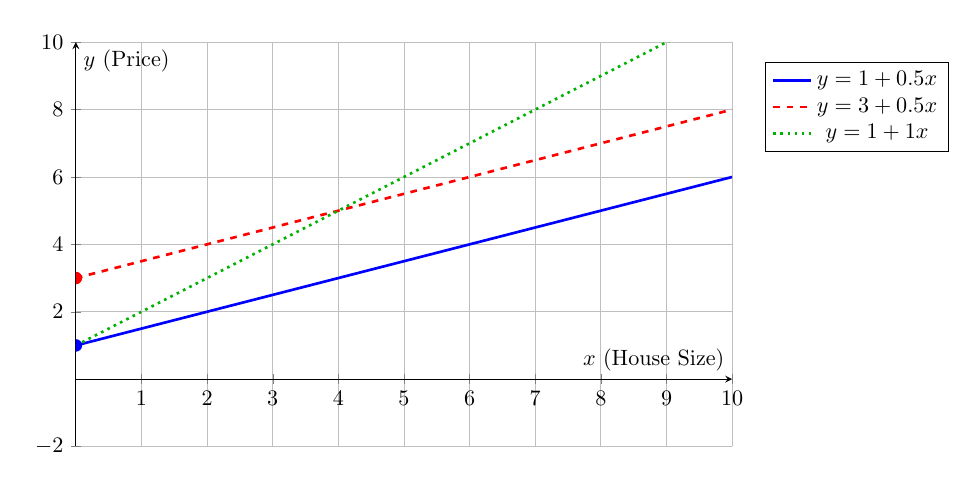
\begin{tikzpicture}[scale=0.8]
    \begin{axis}[
        axis lines = middle,
        xlabel = {$x$ (House Size)},
        ylabel = {$y$ (Price)},
        xmin=0, xmax=10,
        ymin=-2, ymax=10,
        width=12cm,
        height=8cm,
        grid=major,
        legend style={
            at={(1.05,0.95)},
            anchor=north west
        }
    ]

    % Line with beta_0 = 1, beta_1 = 0.5
    \addplot[domain=0:10, samples=2, blue, very thick] {1 + 0.5*x};
    \addlegendentry{$y = 1 + 0.5x$}
    
    % Line with beta_0 = 3, beta_1 = 0.5 (same slope, different intercept)
    \addplot[domain=0:10, samples=2, red, very thick, dashed] {3 + 0.5*x};
    \addlegendentry{$y = 3 + 0.5x$}
    
    % Line with beta_0 = 1, beta_1 = 1 (same intercept, different slope)
    \addplot[domain=0:10, samples=2, green!70!black, very thick, dotted] {1 + 1*x};
    \addlegendentry{$y = 1 + 1x$}
    
    % Mark intercepts
    \node[circle, fill=blue, inner sep=2pt] at (axis cs:0,1) {};
    \node[circle, fill=red, inner sep=2pt] at (axis cs:0,3) {};
    
    \end{axis}
\end{tikzpicture}
\end{center}

Notice how changing $\beta_0$ shifts the line vertically, while changing $\beta_1$ changes the tilt!
\end{geometricintuition}


\subsection{Why a Straight Line?}

\begin{mentalmodel}
You might ask: "Why not a curve? Real data isn't perfectly straight!"

You're absolutely right! But we start with lines for three reasons:

\begin{enumerate}
    \item \textbf{Simplicity:} Lines are the simplest possible model (only 2 parameters!)
    \item \textbf{Interpretability:} The slope has a clear meaning: "increase in $y$ per unit increase in $x$"
    \item \textbf{Building block:} Understanding lines helps us understand more complex models later
\end{enumerate}

Think of it like learning arithmetic before algebra. Lines are our arithmetic!
\end{mentalmodel}

\subsection{The Data: What We Actually Observe}

In the real world, we don't observe the true line. We observe \textbf{noisy data points}.

Suppose we have $n$ observations (data points):
\begin{equation}
    (x_1, y_1), (x_2, y_2), (x_3, y_3), \ldots, (x_n, y_n)
\end{equation}

Each point represents one house: $x_i$ is its size, $y_i$ is its price.

\begin{example}[Our House Price Data]
Here's actual data we'll work with throughout this chapter:

\begin{center}
\begin{tabular}{|c|c|c|c|}
\hline
\textbf{House \#} & \textbf{Size ($x_i$)} & \textbf{Price ($y_i$)} & \textbf{Meaning} \\
\hline
1 & 1000 sq ft & \$200,000 & Small house \\
2 & 1500 sq ft & \$250,000 & Small-medium house \\
3 & 2000 sq ft & \$350,000 & Medium house \\
4 & 2500 sq ft & \$400,000 & Large house \\
5 & 3000 sq ft & \$500,000 & Very large house \\
\hline
\end{tabular}
\end{center}

\textit{Note: We'll work with prices in thousands of dollars ($y$ in \$1000s) to keep numbers manageable.}
\end{example}

\section{Question 2: What Does "Best" Mean?}

\subsection{The Concept of a Residual}

Since our data doesn't fall perfectly on a line, we need to measure how "wrong" any given line is.

\begin{definition}[Residual]
For a given data point $(x_i, y_i)$ and a line with parameters $\beta_0, \beta_1$, the \textbf{residual} is the vertical distance from the point to the line:

\begin{equation}
    e_i = y_i - \hat{y}_i = y_i - (\beta_0 + \beta_1 x_i)
\end{equation}

where $\hat{y}_i = \beta_0 + \beta_1 x_i$ is the \textbf{predicted} value on the line.
\end{definition}
\pagebreak
\begin{geometricintuition}
\textbf{Visualizing Residuals:}

\begin{center}
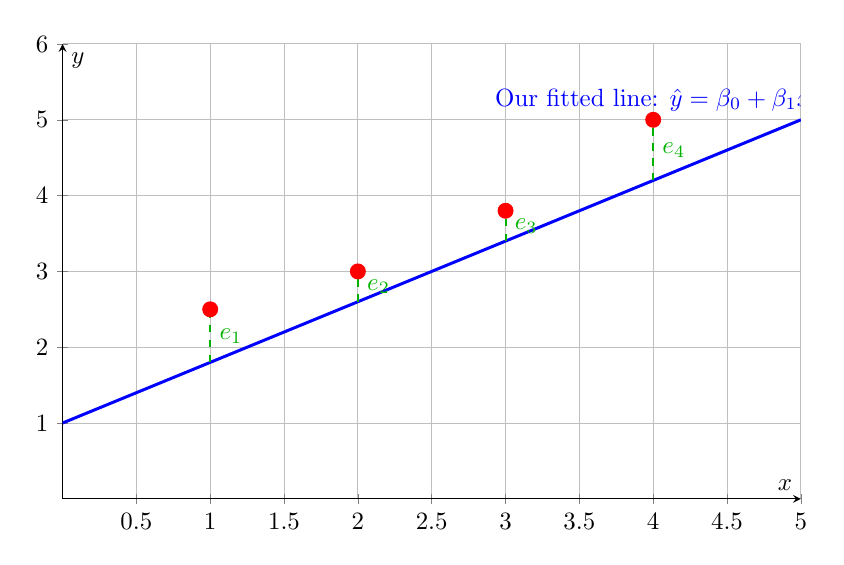
\begin{tikzpicture}[scale=0.9]
    \begin{axis}[
        axis lines = middle,
        xlabel = {$x$},
        ylabel = {$y$},
        xmin=0, xmax=5,
        ymin=0, ymax=6,
        width=12cm,
        height=8cm,
        grid=major
    ]
    
    % The fitted line
    \addplot[domain=0:5, samples=2, blue, very thick] {1 + 0.8*x};
    \node[blue, above] at (axis cs:4,5)
    {Our fitted line: $\hat{y} = \beta_0 + \beta_1 x$};
    
    % Data points
    \addplot[only marks, mark=*, mark size=3pt, red] coordinates {
        (1, 2.5)
        (2, 3)
        (3, 3.8)
        (4, 5)
    };
    
    % Residual lines
    \draw[dashed, thick, green!70!black]
        (axis cs:1, 1.8) -- node[right] {$e_1$} (axis cs:1, 2.5);

    \draw[dashed, thick, green!70!black]
        (axis cs:2, 2.6) -- node[right] {$e_2$} (axis cs:2, 3);

    \draw[dashed, thick, green!70!black]
        (axis cs:3, 3.4) -- node[right] {$e_3$} (axis cs:3, 3.8);

    \draw[dashed, thick, green!70!black]
        (axis cs:4, 4.2) -- node[right] {$e_4$} (axis cs:4, 5);
        
    \end{axis}
\end{tikzpicture}
\end{center}

The green dashed lines show the residuals - how far each point is from our line. Some are positive (point above line), some negative (point below line).
\end{geometricintuition}

\begin{intuition}
Think of residuals as "mistakes" or "errors" our line makes:
\begin{itemize}
    \item If $e_i > 0$: We predicted too low (actual price is higher)
    \item If $e_i < 0$: We predicted too high (actual price is lower)
    \item If $e_i = 0$: Perfect prediction! (rare in real data)
\end{itemize}
\end{intuition}

\subsection{Why We Can't Just Add Up Residuals}

You might think: "Let's just add up all the residuals and make that sum small!"

\begin{equation}
    \text{Total Error} = e_1 + e_2 + e_3 + \cdots + e_n = \sum_{i=1}^{n} e_i
\end{equation}

\textbf{Problem:} Positive and negative errors cancel out!

\begin{example}[The Cancellation Problem]
Suppose we have 3 residuals:
\begin{itemize}
    \item $e_1 = +5$ (we predicted \$5,000 too low)
    \item $e_2 = -3$ (we predicted \$3,000 too high)
    \item $e_3 = -2$ (we predicted \$2,000 too high)
\end{itemize}

Sum = $5 + (-3) + (-2) = 0$

But we're clearly making errors! The sum hides this because errors cancel.
\end{example}

\subsection{The Sum of Squared Errors (SSE)}

\begin{keyidea}
Instead of adding residuals, we \textbf{square} them first, then add:

\begin{equation}
    \text{SSE}(\beta_0, \beta_1) = \sum_{i=1}^{n} e_i^2 = \sum_{i=1}^{n} (y_i - \beta_0 - \beta_1 x_i)^2
\end{equation}

This is also called the \textbf{Residual Sum of Squares (RSS)} or \textbf{Sum of Squared Residuals (SSR)}.
\end{keyidea}

\begin{mentalmodel}
Why squares? Three excellent reasons:

\begin{enumerate}
    \item \textbf{Always positive:} $e_i^2 \geq 0$, so no cancellation!
    \item \textbf{Penalizes large errors more:} An error of 10 contributes $10^2 = 100$, while two errors of 5 contribute only $2 \times 5^2 = 50$. We really don't want big mistakes!
    \item \textbf{Beautiful mathematics:} Squares give us calculus that works out perfectly (you'll see!)
\end{enumerate}

Think of it like: "We want small errors, but we REALLY don't want big errors!"
\end{mentalmodel}

\begin{definition}[Mean Squared Error (MSE)]
Sometimes we divide by $n$ to get the average squared error:
\begin{equation}
    \text{MSE}(\beta_0, \beta_1) = \frac{1}{n}\sum_{i=1}^{n} (y_i - \beta_0 - \beta_1 x_i)^2
\end{equation}

MSE and SSE are proportional (MSE = SSE/$n$), so minimizing one minimizes the other.
\end{definition}

\subsection{Our Goal: Ordinary Least Squares (OLS)}

\begin{importantbox}
\textbf{The Least Squares Principle:}

Find the values of $\beta_0$ and $\beta_1$ that minimize the Sum of Squared Errors:

\begin{equation}
    (\hat{\beta}_0, \hat{\beta}_1) = \arg\min_{\beta_0, \beta_1} \sum_{i=1}^{n} (y_i - \beta_0 - \beta_1 x_i)^2
\end{equation}

The hat notation $\hat{\beta}$ means "our estimate" of the true parameters.

This is called \textbf{Ordinary Least Squares (OLS)} regression.
\end{importantbox}

\section{Question 3: How Do We Find the Best Line?}

\subsection{The Power of Calculus}

\begin{mentalmodel}
Imagine you're hiking in foggy mountains, trying to find the lowest valley. How do you do it?

\textbf{Strategy:} Look at the ground's slope. If it's sloping down to your left, go left. If it's sloping down to your right, go right. When the slope is zero (flat), you've found the bottom!

This is exactly what calculus does for us! The derivative tells us the "slope," and we find where it's zero.
\end{mentalmodel}

\subsection{Step 1: Take Partial Derivatives}

We have a function of two variables: $\text{SSE}(\beta_0, \beta_1)$. To find the minimum, we take partial derivatives with respect to both variables and set them to zero.

\begin{theorem}[Necessary Conditions for Minimum]
At a minimum, both partial derivatives must equal zero:
\begin{align}
    \frac{\partial \text{SSE}}{\partial \beta_0} &= 0 \\
    \frac{\partial \text{SSE}}{\partial \beta_1} &= 0
\end{align}
\end{theorem}

\subsubsection{Derivative with Respect to $\beta_0$}

Let's compute this carefully, step by step:

\begin{align}
    \text{SSE}(\beta_0, \beta_1) &= \sum_{i=1}^{n} (y_i - \beta_0 - \beta_1 x_i)^2 \\
\end{align}

Taking the derivative using the chain rule:
\begin{align}
    \frac{\partial \text{SSE}}{\partial \beta_0} &= \frac{\partial}{\partial \beta_0} \sum_{i=1}^{n} (y_i - \beta_0 - \beta_1 x_i)^2 \\
    &= \sum_{i=1}^{n} \frac{\partial}{\partial \beta_0} (y_i - \beta_0 - \beta_1 x_i)^2 \\
    &= \sum_{i=1}^{n} 2(y_i - \beta_0 - \beta_1 x_i) \cdot \frac{\partial}{\partial \beta_0}(y_i - \beta_0 - \beta_1 x_i) \\
    &= \sum_{i=1}^{n} 2(y_i - \beta_0 - \beta_1 x_i) \cdot (-1) \\
    &= -2\sum_{i=1}^{n} (y_i - \beta_0 - \beta_1 x_i)
\end{align}

\begin{remark}[Understanding Each Step]
\begin{itemize}
    \item Line 2: The derivative of a sum is the sum of derivatives
    \item Line 3: Chain rule: derivative of $(f(x))^2$ is $2f(x) \cdot f'(x)$
    \item Line 4: The derivative of $(y_i - \beta_0 - \beta_1 x_i)$ with respect to $\beta_0$ is $-1$ (since $y_i$ and $x_i$ are constants)
\end{itemize}
\end{remark}

Setting this equal to zero:
\begin{align}
    -2\sum_{i=1}^{n} (y_i - \beta_0 - \beta_1 x_i) &= 0 \\
    \sum_{i=1}^{n} (y_i - \beta_0 - \beta_1 x_i) &= 0 \\
    \sum_{i=1}^{n} y_i - \sum_{i=1}^{n}\beta_0 - \sum_{i=1}^{n}\beta_1 x_i &= 0 \\
    \sum_{i=1}^{n} y_i - n\beta_0 - \beta_1\sum_{i=1}^{n} x_i &= 0
\end{align}

This gives us our \textbf{first equation}:
\begin{equation}\label{eq:normal1}
    \boxed{n\beta_0 + \beta_1\sum_{i=1}^{n} x_i = \sum_{i=1}^{n} y_i}
\end{equation}

\subsubsection{Derivative with Respect to $\beta_1$}

Now for $\beta_1$:

\begin{align}
    \frac{\partial \text{SSE}}{\partial \beta_1} &= \frac{\partial}{\partial \beta_1} \sum_{i=1}^{n} (y_i - \beta_0 - \beta_1 x_i)^2 \\
    &= \sum_{i=1}^{n} 2(y_i - \beta_0 - \beta_1 x_i) \cdot \frac{\partial}{\partial \beta_1}(y_i - \beta_0 - \beta_1 x_i) \\
    &= \sum_{i=1}^{n} 2(y_i - \beta_0 - \beta_1 x_i) \cdot (-x_i) \\
    &= -2\sum_{i=1}^{n} x_i(y_i - \beta_0 - \beta_1 x_i)
\end{align}

Setting equal to zero:
\begin{align}
    -2\sum_{i=1}^{n} x_i(y_i - \beta_0 - \beta_1 x_i) &= 0 \\
    \sum_{i=1}^{n} x_i(y_i - \beta_0 - \beta_1 x_i) &= 0 \\
    \sum_{i=1}^{n} x_i y_i - \beta_0\sum_{i=1}^{n} x_i - \beta_1\sum_{i=1}^{n} x_i^2 &= 0
\end{align}

This gives us our \textbf{second equation}:
\begin{equation}\label{eq:normal2}
    \boxed{\beta_0\sum_{i=1}^{n} x_i + \beta_1\sum_{i=1}^{n} x_i^2 = \sum_{i=1}^{n} x_i y_i}
\end{equation}

\subsection{Step 2: Solve the System of Equations}

We now have two equations with two unknowns:
\begin{align}
    n\beta_0 + \beta_1\sum x_i &= \sum y_i \tag{Equation 1}\\
    \beta_0\sum x_i + \beta_1\sum x_i^2 &= \sum x_i y_i \tag{Equation 2}
\end{align}

Let's introduce notation to make this cleaner:
\begin{align}
    S_x &= \sum_{i=1}^{n} x_i \quad \text{(sum of all $x$ values)} \\
    S_y &= \sum_{i=1}^{n} y_i \quad \text{(sum of all $y$ values)} \\
    S_{xx} &= \sum_{i=1}^{n} x_i^2 \quad \text{(sum of squared $x$ values)} \\
    S_{xy} &= \sum_{i=1}^{n} x_i y_i \quad \text{(sum of products)}
\end{align}

Our equations become:
\begin{align}
    n\beta_0 + \beta_1 S_x &= S_y \tag{1}\\
    \beta_0 S_x + \beta_1 S_{xx} &= S_{xy} \tag{2}
\end{align}

\subsubsection{Solving for $\beta_0$ Using Means}

From equation (1), divide both sides by $n$:
\begin{equation}
    \beta_0 + \beta_1 \frac{S_x}{n} = \frac{S_y}{n}
\end{equation}

Notice that $\frac{S_x}{n} = \bar{x}$ (the mean of $x$) and $\frac{S_y}{n} = \bar{y}$ (the mean of $y$):

\begin{equation}
    \beta_0 = \bar{y} - \beta_1 \bar{x}
\end{equation}

\begin{geometricintuition}
\textbf{Beautiful Geometric Fact:}

The regression line \textbf{always passes through the point} $(\bar{x}, \bar{y})$ - the center of mass of the data!

Why? Because when $x = \bar{x}$:
\begin{align}
    \hat{y} &= \beta_0 + \beta_1 \bar{x} \\
    &= (\bar{y} - \beta_1\bar{x}) + \beta_1\bar{x} \\
    &= \bar{y} \quad \checkmark
\end{align}

This is like a balance point - the line pivots through the center!
\end{geometricintuition}

\subsubsection{Solving for $\beta_1$}

Substitute $\beta_0 = \bar{y} - \beta_1\bar{x}$ into equation (2):

\begin{align}
    (\bar{y} - \beta_1\bar{x})S_x + \beta_1 S_{xx} &= S_{xy} \\
    \bar{y}S_x - \beta_1\bar{x}S_x + \beta_1 S_{xx} &= S_{xy} \\
    \beta_1(S_{xx} - \bar{x}S_x) &= S_{xy} - \bar{y}S_x \\
    \beta_1 &= \frac{S_{xy} - \bar{y}S_x}{S_{xx} - \bar{x}S_x}
\end{align}

Now, let's simplify. Note that:
\begin{align}
    \bar{x}S_x &= \bar{x} \cdot n\bar{x} = n\bar{x}^2 \\
    \bar{y}S_x &= \bar{y} \cdot n\bar{x} = n\bar{x}\bar{y}
\end{align}

So:
\begin{equation}
    \beta_1 = \frac{S_{xy} - n\bar{x}\bar{y}}{S_{xx} - n\bar{x}^2}
\end{equation}

\begin{theorem}[The Most Beautiful Form]
With some algebra (expanding and regrouping), this becomes:

\begin{equation}
    \boxed{\beta_1 = \frac{\sum_{i=1}^{n}(x_i - \bar{x})(y_i - \bar{y})}{\sum_{i=1}^{n}(x_i - \bar{x})^2}}
\end{equation}

And:
\begin{equation}
    \boxed{\beta_0 = \bar{y} - \beta_1\bar{x}}
\end{equation}
\end{theorem}

\begin{proof}[Why These Forms are Equivalent]
Let's verify the numerator:
\begin{align}
    \sum(x_i - \bar{x})(y_i - \bar{y}) &= \sum(x_i y_i - x_i\bar{y} - \bar{x}y_i + \bar{x}\bar{y}) \\
    &= \sum x_i y_i - \bar{y}\sum x_i - \bar{x}\sum y_i + n\bar{x}\bar{y} \\
    &= S_{xy} - \bar{y}(n\bar{x}) - \bar{x}(n\bar{y}) + n\bar{x}\bar{y} \\
    &= S_{xy} - n\bar{x}\bar{y} - n\bar{x}\bar{y} + n\bar{x}\bar{y} \\
    &= S_{xy} - n\bar{x}\bar{y} \quad \checkmark
\end{align}

Similarly for the denominator:
\begin{align}
    \sum(x_i - \bar{x})^2 &= \sum(x_i^2 - 2x_i\bar{x} + \bar{x}^2) \\
    &= \sum x_i^2 - 2\bar{x}\sum x_i + n\bar{x}^2 \\
    &= S_{xx} - 2\bar{x}(n\bar{x}) + n\bar{x}^2 \\
    &= S_{xx} - 2n\bar{x}^2 + n\bar{x}^2 \\
    &= S_{xx} - n\bar{x}^2 \quad \checkmark
\end{align}
\end{proof}

\subsection{Understanding the Formulas}

\begin{intuition}
Let's understand what $\beta_1$ means:

\begin{equation}
    \beta_1 = \frac{\sum(x_i - \bar{x})(y_i - \bar{y})}{\sum(x_i - \bar{x})^2}
\end{equation}

\textbf{Numerator:} Measures how $x$ and $y$ vary \textit{together}
\begin{itemize}
    \item When $x_i > \bar{x}$ and $y_i > \bar{y}$: positive contribution (both above average)
    \item When $x_i < \bar{x}$ and $y_i < \bar{y}$: positive contribution (both below average)
    \item When they go opposite directions: negative contribution
\end{itemize}

\textbf{Denominator:} Measures how much $x$ varies by itself

\textbf{The ratio:} "For every unit increase in $x$, how much does $y$ increase?"
\end{intuition}

\begin{remark}[Connection to Covariance and Variance]
The formula can also be written as:
\begin{equation}
    \beta_1 = \frac{\text{Cov}(x, y)}{\text{Var}(x)} = \frac{\frac{1}{n}\sum(x_i-\bar{x})(y_i-\bar{y})}{\frac{1}{n}\sum(x_i-\bar{x})^2}
\end{equation}

This shows $\beta_1$ is really about the relationship between variability in $x$ and variability in $y$!
\end{remark}

\section{Complete Numerical Example: Step-by-Step}

Let's work through our house price example with \textbf{every single calculation} shown.

\begin{example}[House Prices - Complete Solution]

\textbf{Given Data:}
\begin{center}
\begin{tabular}{|c|c|c|}
\hline
House ($i$) & Size ($x_i$, sq ft) & Price ($y_i$, \$1000s) \\
\hline
1 & 1000 & 200 \\
2 & 1500 & 250 \\
3 & 2000 & 350 \\
4 & 2500 & 400 \\
5 & 3000 & 500 \\
\hline
\end{tabular}
\end{center}

\textbf{STEP 1: Calculate Basic Sums}

\begin{align}
    n &= 5 \\
    S_x &= \sum x_i = 1000 + 1500 + 2000 + 2500 + 3000 = 10000 \\
    S_y &= \sum y_i = 200 + 250 + 350 + 400 + 500 = 1700
\end{align}

\textbf{STEP 2: Calculate Means}

\begin{align}
    \bar{x} &= \frac{S_x}{n} = \frac{10000}{5} = 2000 \text{ sq ft} \\
    \bar{y} &= \frac{S_y}{n} = \frac{1700}{5} = 340 \text{ (\$1000s) = \$340,000}
\end{align}

\textbf{STEP 3: Create a Detailed Calculation Table}

\begin{center}
\small
\begin{tabular}{|c|c|c|c|c|c|c|c|}
\hline
$i$ & $x_i$ & $y_i$ & $x_i - \bar{x}$ & $y_i - \bar{y}$ & $(x_i-\bar{x})(y_i-\bar{y})$ & $(x_i-\bar{x})^2$ & $x_i y_i$ \\
\hline
1 & 1000 & 200 & -1000 & -140 & 140000 & 1000000 & 200000 \\
2 & 1500 & 250 & -500 & -90 & 45000 & 250000 & 375000 \\
3 & 2000 & 350 & 0 & 10 & 0 & 0 & 700000 \\
4 & 2500 & 400 & 500 & 60 & 30000 & 250000 & 1000000 \\
5 & 3000 & 500 & 1000 & 160 & 160000 & 1000000 & 1500000 \\
\hline
\multicolumn{5}{|r|}{\textbf{Sums:}} & \textbf{375000} & \textbf{2500000} & \textbf{3775000} \\
\hline
\end{tabular}
\end{center}

Let me explain each column:
\begin{itemize}
    \item Column 4: Deviation from mean size. House 3 is exactly average (0), House 5 is 1000 sq ft above average
    \item Column 5: Deviation from mean price. House 1 is \$140,000 below average
    \item Column 6: Product of deviations. House 1: both below average, so product is positive
    \item Column 7: Squared deviations in size
    \item Column 8: Product of size and price (needed for verification)
\end{itemize}

\textbf{STEP 4: Calculate $\beta_1$ (the slope)}

Using our formula:
\begin{align}
    \beta_1 &= \frac{\sum(x_i - \bar{x})(y_i - \bar{y})}{\sum(x_i - \bar{x})^2} \\
    &= \frac{375000}{2500000} \\
    &= 0.15
\end{align}

\textbf{Interpretation:} For each additional square foot, the price increases by \$0.15 thousand = \textbf{\$150}.

\textbf{STEP 5: Calculate $\beta_0$ (the intercept)}

\begin{align}
    \beta_0 &= \bar{y} - \beta_1 \bar{x} \\
    &= 340 - 0.15(2000) \\
    &= 340 - 300 \\
    &= 40
\end{align}

\textbf{Interpretation:} The base price (when size = 0) is \$40,000. (This is extrapolation and may not be meaningful in reality!)

\textbf{STEP 6: Write the Final Regression Equation}

\begin{equation}
    \boxed{\hat{y} = 40 + 0.15x}
\end{equation}

Or in full words:
\begin{equation}
    \text{Price (\$1000s)} = 40 + 0.15 \times \text{Size (sq ft)}
\end{equation}

\textbf{STEP 7: Verify - Line Passes Through $(\bar{x}, \bar{y})$}

\begin{align}
    \hat{y} &= 40 + 0.15(2000) \\
    &= 40 + 300 \\
    &= 340 = \bar{y} \quad \checkmark
\end{align}

Perfect! The line goes through $(2000, 340)$ as promised.

\textbf{STEP 8: Make Predictions}

\textit{Example 1:} What's the predicted price for a 2200 sq ft house?
\begin{align}
    \hat{y} &= 40 + 0.15(2200) \\
    &= 40 + 330 \\
    &= 370 \text{ thousand dollars} \\
    &= \$370,000
\end{align}

\textit{Example 2:} What about a 1750 sq ft house?
\begin{align}
    \hat{y} &= 40 + 0.15(1750) \\
    &= 40 + 262.5 \\
    &= 302.5 \\
    &= \$302,500
\end{align}

\textbf{STEP 9: Calculate Residuals (Errors)}

For each original data point, compare actual vs predicted:

\begin{center}
\begin{tabular}{|c|c|c|c|c|c|}
\hline
$i$ & $x_i$ & $y_i$ & $\hat{y}_i = 40 + 0.15x_i$ & $e_i = y_i - \hat{y}_i$ & $e_i^2$ \\
\hline
1 & 1000 & 200 & $40 + 150 = 190$ & $200 - 190 = 10$ & 100 \\
2 & 1500 & 250 & $40 + 225 = 265$ & $250 - 265 = -15$ & 225 \\
3 & 2000 & 350 & $40 + 300 = 340$ & $350 - 340 = 10$ & 100 \\
4 & 2500 & 400 & $40 + 375 = 415$ & $400 - 415 = -15$ & 225 \\
5 & 3000 & 500 & $40 + 450 = 490$ & $500 - 490 = 10$ & 100 \\
\hline
\multicolumn{4}{|r|}{\textbf{Sum of residuals:}} & \textbf{0} & \\
\multicolumn{5}{|r|}{\textbf{SSE =}} & \textbf{750} \\
\hline
\end{tabular}
\end{center}

\textbf{Important observation:} The sum of residuals is exactly zero! This always happens with OLS (it's a mathematical property).

\textbf{STEP 10: Calculate Error Metrics}

\textbf{Sum of Squared Errors:}
\begin{equation}
    \text{SSE} = 100 + 225 + 100 + 225 + 100 = 750
\end{equation}

\textbf{Mean Squared Error:}
\begin{equation}
    \text{MSE} = \frac{750}{5} = 150
\end{equation}

\textbf{Root Mean Squared Error (RMSE):}
\begin{equation}
    \text{RMSE} = \sqrt{150} \approx 12.25 \text{ thousand dollars} = \$12,250
\end{equation}

\textbf{Interpretation:} On average, our predictions are off by about \$12,250. Given houses cost hundreds of thousands, this is pretty good!

\end{example}

\section{Measuring Model Quality: $R^2$}

\subsection{What is $R^2$?}

\begin{mentalmodel}
Imagine you're explaining house prices to someone who knows nothing. You'd probably say: "On average, houses cost \$340,000."

That's your baseline - just predicting the mean. How much better does our regression line do compared to that baseline?

$R^2$ answers exactly this question!
\end{mentalmodel}

\begin{definition}[Total Sum of Squares (SST)]
This measures total variability in $y$ if we just predicted $\bar{y}$ for everything:

\begin{equation}
    \text{SST} = \sum_{i=1}^{n} (y_i - \bar{y})^2
\end{equation}

It's the "total error" of the naive "always predict the mean" strategy.
\end{definition}

\begin{definition}[Coefficient of Determination ($R^2$)]
\begin{equation}
    R^2 = 1 - \frac{\text{SSE}}{\text{SST}} = 1 - \frac{\sum(y_i - \hat{y}_i)^2}{\sum(y_i - \bar{y})^2}
\end{equation}

$R^2$ is the proportion of variance in $y$ explained by our model.
\end{definition}

\begin{intuition}
Think of it as:
\begin{align}
    R^2 &= 1 - \frac{\text{Error with our model}}{\text{Error with just the mean}} \\
    &= \frac{\text{Improvement from using model}}{\text{Total variance to explain}}
\end{align}

\begin{itemize}
    \item $R^2 = 0$: Model is useless (no better than predicting $\bar{y}$)
    \item $R^2 = 1$: Perfect fit (all points exactly on the line)
    \item $R^2 = 0.5$: Model explains 50\% of variance
    \item $R^2 = 0.9$: Model explains 90\% of variance (very good!)
\end{itemize}
\end{intuition}

\subsection{Calculating $R^2$ for Our Example}

\begin{example}[Computing $R^2$ for House Prices]

\textbf{Step 1: Calculate SST}

\begin{center}
\begin{tabular}{|c|c|c|c|c|}
\hline
$i$ & $y_i$ & $\bar{y}$ & $y_i - \bar{y}$ & $(y_i - \bar{y})^2$ \\
\hline
1 & 200 & 340 & -140 & 19600 \\
2 & 250 & 340 & -90 & 8100 \\
3 & 350 & 340 & 10 & 100 \\
4 & 400 & 340 & 60 & 3600 \\
5 & 500 & 340 & 160 & 25600 \\
\hline
\multicolumn{4}{|r|}{\textbf{SST =}} & \textbf{57000} \\
\hline
\end{tabular}
\end{center}

\textbf{Step 2: We already have SSE = 750}

\textbf{Step 3: Calculate $R^2$}

\begin{align}
    R^2 &= 1 - \frac{\text{SSE}}{\text{SST}} \\
    &= 1 - \frac{750}{57000} \\
    &= 1 - 0.01316 \\
    &\approx 0.987 \\
    &= 98.7\%
\end{align}

\textbf{Interpretation:} Our simple linear model explains \textbf{98.7\%} of the variance in house prices! That's excellent! Only 1.3\% of the variation is left unexplained.

\end{example}

\begin{remark}[Alternative Formula for $R^2$]
In simple linear regression, $R^2$ equals the square of the correlation coefficient:
\begin{equation}
    R^2 = r^2_{xy}
\end{equation}

where:
\begin{equation}
    r_{xy} = \frac{\sum(x_i - \bar{x})(y_i - \bar{y})}{\sqrt{\sum(x_i - \bar{x})^2 \cdot \sum(y_i - \bar{y})^2}}
\end{equation}

For our data: $r_{xy} = \frac{375000}{\sqrt{2500000 \times 57000}} \approx 0.993$, so $R^2 = 0.993^2 \approx 0.987$ $\checkmark$

\end{remark}

\section{The Geometry of Least Squares (Advanced)}

\subsection{Matrix Formulation}

\begin{keyidea}
Everything we've done can be expressed beautifully using matrices and vectors. This viewpoint reveals deep geometric structure!
\end{keyidea}

Define:
\begin{equation}
    \mathbf{y} = \begin{bmatrix} y_1 \\ y_2 \\ \vdots \\ y_n \end{bmatrix}, \quad
    \mathbf{X} = \begin{bmatrix} 1 & x_1 \\ 1 & x_2 \\ \vdots & \vdots \\ 1 & x_n \end{bmatrix}, \quad
    \boldsymbol{\beta} = \begin{bmatrix} \beta_0 \\ \beta_1 \end{bmatrix}
\end{equation}

Our model is:
\begin{equation}
    \mathbf{y} = \mathbf{X}\boldsymbol{\beta} + \boldsymbol{\epsilon}
\end{equation}

Predictions:
\begin{equation}
    \hat{\mathbf{y}} = \mathbf{X}\boldsymbol{\beta}
\end{equation}

Residuals:
\begin{equation}
    \mathbf{e} = \mathbf{y} - \mathbf{X}\boldsymbol{\beta}
\end{equation}

SSE:
\begin{equation}
    \text{SSE} = ||\mathbf{e}||^2 = \mathbf{e}^T\mathbf{e} = (\mathbf{y} - \mathbf{X}\boldsymbol{\beta})^T(\mathbf{y} - \mathbf{X}\boldsymbol{\beta})
\end{equation}

\subsection{The Projection Interpretation}

\begin{geometricintuition}
Here's the profound insight:

Think of $\mathbf{y} = [y_1, y_2, \ldots, y_n]^T$ as a vector in $n$-dimensional space.

The columns of $\mathbf{X}$ span a 2-dimensional subspace (the "column space" of $\mathbf{X}$).

$\hat{\mathbf{y}} = \mathbf{X}\boldsymbol{\beta}$ lives in this subspace.

\textbf{The best approximation to $\mathbf{y}$ in the column space is its orthogonal projection!}

The residual $\mathbf{e} = \mathbf{y} - \hat{\mathbf{y}}$ is perpendicular to the column space.
\end{geometricintuition}

\begin{theorem}[Normal Equations via Orthogonality]
At the minimum, the residual vector is orthogonal to the column space:
\begin{equation}
    \mathbf{X}^T\mathbf{e} = \mathbf{0}
\end{equation}

This gives:
\begin{align}
    \mathbf{X}^T(\mathbf{y} - \mathbf{X}\boldsymbol{\beta}) &= \mathbf{0} \\
    \mathbf{X}^T\mathbf{y} - \mathbf{X}^T\mathbf{X}\boldsymbol{\beta} &= \mathbf{0} \\
    \mathbf{X}^T\mathbf{X}\boldsymbol{\beta} &= \mathbf{X}^T\mathbf{y}
\end{align}

These are the \textbf{normal equations}!
\end{theorem}

\begin{theorem}[Closed-Form Solution]
The least squares solution is:
\begin{equation}
    \boxed{\boldsymbol{\beta} = (\mathbf{X}^T\mathbf{X})^{-1}\mathbf{X}^T\mathbf{y}}
\end{equation}

The matrix $\mathbf{P} = \mathbf{X}(\mathbf{X}^T\mathbf{X})^{-1}\mathbf{X}^T$ is the \textbf{projection matrix}.
\end{theorem}

\subsection{Numerical Verification with Matrices}

\begin{example}[Matrix Calculation for Our Data]

\begin{equation}
    \mathbf{X} = \begin{bmatrix} 
        1 & 1000 \\ 
        1 & 1500 \\ 
        1 & 2000 \\ 
        1 & 2500 \\ 
        1 & 3000 
    \end{bmatrix}, \quad
    \mathbf{y} = \begin{bmatrix} 
        200 \\ 
        250 \\ 
        350 \\ 
        400 \\ 
        500 
    \end{bmatrix}
\end{equation}

\textbf{Compute $\mathbf{X}^T\mathbf{X}$:}

\begin{align}
    \mathbf{X}^T\mathbf{X} &= \begin{bmatrix} 1 & 1 & 1 & 1 & 1 \\ 1000 & 1500 & 2000 & 2500 & 3000 \end{bmatrix}
    \begin{bmatrix} 1 & 1000 \\ 1 & 1500 \\ 1 & 2000 \\ 1 & 2500 \\ 1 & 3000 \end{bmatrix} \\
    &= \begin{bmatrix} 
        1+1+1+1+1 & 1000+1500+2000+2500+3000 \\
        1000+1500+2000+2500+3000 & 1000^2+1500^2+2000^2+2500^2+3000^2
    \end{bmatrix} \\
    &= \begin{bmatrix} 5 & 10000 \\ 10000 & 22500000 \end{bmatrix}
\end{align}

\textbf{Compute $\mathbf{X}^T\mathbf{y}$:}

\begin{align}
    \mathbf{X}^T\mathbf{y} &= \begin{bmatrix} 1 & 1 & 1 & 1 & 1 \\ 1000 & 1500 & 2000 & 2500 & 3000 \end{bmatrix}
    \begin{bmatrix} 200 \\ 250 \\ 350 \\ 400 \\ 500 \end{bmatrix} \\
    &= \begin{bmatrix} 200+250+350+400+500 \\ 1000(200)+1500(250)+2000(350)+2500(400)+3000(500) \end{bmatrix} \\
    &= \begin{bmatrix} 1700 \\ 3775000 \end{bmatrix}
\end{align}

\textbf{Compute $(\mathbf{X}^T\mathbf{X})^{-1}$:}

For a $2 \times 2$ matrix $\begin{bmatrix} a & b \\ c & d \end{bmatrix}$, the inverse is:
\begin{equation}
    \frac{1}{ad - bc}\begin{bmatrix} d & -b \\ -c & a \end{bmatrix}
\end{equation}

\begin{align}
    \det(\mathbf{X}^T\mathbf{X}) &= 5(22500000) - 10000(10000) \\
    &= 112500000 - 100000000 \\
    &= 12500000
\end{align}

\begin{align}
    (\mathbf{X}^T\mathbf{X})^{-1} &= \frac{1}{12500000}\begin{bmatrix} 22500000 & -10000 \\ -10000 & 5 \end{bmatrix} \\
    &= \begin{bmatrix} 1.8 & -0.0008 \\ -0.0008 & 0.0000004 \end{bmatrix}
\end{align}

\textbf{Compute $\boldsymbol{\beta}$:}

\begin{align}
    \boldsymbol{\beta} &= (\mathbf{X}^T\mathbf{X})^{-1}\mathbf{X}^T\mathbf{y} \\
    &= \begin{bmatrix} 1.8 & -0.0008 \\ -0.0008 & 0.0000004 \end{bmatrix}
    \begin{bmatrix} 1700 \\ 3775000 \end{bmatrix} \\
    &= \begin{bmatrix} 
        1.8(1700) - 0.0008(3775000) \\
        -0.0008(1700) + 0.0000004(3775000)
    \end{bmatrix} \\
    &= \begin{bmatrix} 
        3060 - 3020 \\
        -1.36 + 1.51
    \end{bmatrix} \\
    &= \begin{bmatrix} 40 \\ 0.15 \end{bmatrix}
\end{align}

So $\beta_0 = 40$ and $\beta_1 = 0.15$, exactly as before! $\checkmark$

\end{example}

\section{Assumptions of Linear Regression}

\begin{importantbox}
For our formulas to be valid and inferences to be correct, we assume:

\begin{enumerate}
    \item \textbf{Linearity:} The true relationship is linear: $y = \beta_0 + \beta_1 x + \epsilon$
    \item \textbf{Independence:} Observations $(x_i, y_i)$ are independent
    \item \textbf{Homoscedasticity:} Constant variance: $\text{Var}(\epsilon_i) = \sigma^2$ for all $i$
    \item \textbf{Normality:} Errors are normally distributed: $\epsilon_i \sim N(0, \sigma^2)$ (needed for inference, not just fitting)
\end{enumerate}
\end{importantbox}

\begin{mentalmodel}
Think of these as the "rules of the game":
\begin{itemize}
    \item If violated, our formulas might give wrong answers
    \item Always check assumptions before trusting your model!
    \item Plotting residuals helps diagnose violations
\end{itemize}
\end{mentalmodel}

\section{Summary and Key Takeaways}

\begin{keyidea}
\textbf{What We Learned:}

\begin{enumerate}
    \item \textbf{The Model:} $y = \beta_0 + \beta_1 x + \epsilon$ (a straight line)
    
    \item \textbf{The Criterion:} Minimize $\text{SSE} = \sum(y_i - \beta_0 - \beta_1 x_i)^2$
    
    \item \textbf{The Solution:}
    \begin{align}
        \beta_1 &= \frac{\sum(x_i - \bar{x})(y_i - \bar{y})}{\sum(x_i - \bar{x})^2} \\
        \beta_0 &= \bar{y} - \beta_1\bar{x}
    \end{align}
    
    \item \textbf{Key Properties:}
    \begin{itemize}
        \item Line passes through $(\bar{x}, \bar{y})$
        \item Sum of residuals = 0
        \item $R^2$ measures goodness of fit
    \end{itemize}
    
    \item \textbf{Geometric View:} OLS = orthogonal projection onto column space of $\mathbf{X}$
\end{enumerate}
\end{keyidea}

\section{Practice Problems}

\begin{example}[Problem 1: Study Hours vs Exam Score]
A teacher collects data on study hours and exam scores:

\begin{center}
\begin{tabular}{|c|c|}
\hline
Study Hours ($x$) & Exam Score ($y$) \\
\hline
2 & 65 \\
4 & 75 \\
6 & 82 \\
8 & 90 \\
\hline
\end{tabular}
\end{center}

Find the regression line and predict the score for a student who studies 5 hours.

\textbf{Solution:} (Work through this yourself using our method!)
\begin{align}
    \bar{x} &= 5, \quad \bar{y} = 78 \\
    \beta_1 &= \frac{(2-5)(65-78) + (4-5)(75-78) + (6-5)(82-78) + (8-5)(90-78)}{(2-5)^2 + (4-5)^2 + (6-5)^2 + (8-5)^2} \\
    &= \frac{39 + 3 + 4 + 36}{9 + 1 + 1 + 9} = \frac{82}{20} = 4.1 \\
    \beta_0 &= 78 - 4.1(5) = 57.5 \\
    \hat{y} &= 57.5 + 4.1x
\end{align}

For 5 hours: $\hat{y} = 57.5 + 4.1(5) = 78$
\end{example}


\chapter{Multiple Linear Regression}

\section{From One Variable to Many}

\begin{mentalmodel}
In Chapter 1, we used only house \textbf{size} to predict price. But in reality, price depends on many factors:
\begin{itemize}
    \item Size (square feet)
    \item Age of the house
    \item Number of bedrooms
    \item Location (distance to city center)
    \item Number of bathrooms
    \item Condition/quality rating
\end{itemize}

Multiple linear regression lets us use \textbf{all these features simultaneously} to make better predictions!
\end{mentalmodel}

\subsection{Why Multiple Regression?}

\begin{example}[The Problem with Simple Regression]
Suppose you only use size to predict price:
\begin{equation}
    \text{Price} = \beta_0 + \beta_1 \times \text{Size}
\end{equation}

Two houses both 2000 sq ft:
\begin{itemize}
    \item House A: New (2 years old), 4 bedrooms → Sells for \$450,000
    \item House B: Old (30 years old), 2 bedrooms → Sells for \$300,000
\end{itemize}

Simple regression predicts the \textbf{same price} for both! We need more variables to capture these differences.
\end{example}

\section{The Multiple Linear Regression Model}

\subsection{Mathematical Formulation}

\begin{definition}[Multiple Linear Regression Model]
We have $p$ predictor variables (features): $x_1, x_2, \ldots, x_p$

The model is:
\begin{equation}
    y = \beta_0 + \beta_1 x_1 + \beta_2 x_2 + \cdots + \beta_p x_p + \epsilon
\end{equation}

where:
\begin{itemize}
    \item $y$ is the response (output) variable
    \item $x_1, \ldots, x_p$ are the predictor (input) variables
    \item $\beta_0$ is the intercept
    \item $\beta_1, \ldots, \beta_p$ are the coefficients (slopes)
    \item $\epsilon$ is the error term
\end{itemize}
\end{definition}

\begin{example}[House Price Model with 3 Features]
\begin{align}
    \text{Price} = &\beta_0 + \beta_1 \times \text{Size} + \beta_2 \times \text{Age} \\
    &+ \beta_3 \times \text{Bedrooms} + \epsilon
\end{align}

If we estimate:
\begin{itemize}
    \item $\beta_0 = 50$ (thousands of dollars)
    \item $\beta_1 = 0.15$ (per sq ft)
    \item $\beta_2 = -2$ (per year of age)
    \item $\beta_3 = 25$ (per bedroom)
\end{itemize}

Then:
\begin{align}
    \text{Price} = 50 + 0.15 \times \text{Size} - 2 \times \text{Age} + 25 \times \text{Bedrooms}
\end{align}
\end{example}

\subsection{Matrix Notation - The Compact Form}

For $n$ observations, we can write everything using matrices:

\begin{equation}
    \mathbf{y} = \mathbf{X}\boldsymbol{\beta} + \boldsymbol{\epsilon}
\end{equation}

where:

\begin{equation}
    \mathbf{y} = \begin{bmatrix} y_1 \\ y_2 \\ \vdots \\ y_n \end{bmatrix}_{n \times 1}, \quad
    \mathbf{X} = \begin{bmatrix} 
        1 & x_{11} & x_{12} & \cdots & x_{1p} \\
        1 & x_{21} & x_{22} & \cdots & x_{2p} \\
        \vdots & \vdots & \vdots & \ddots & \vdots \\
        1 & x_{n1} & x_{n2} & \cdots & x_{np}
    \end{bmatrix}_{n \times (p+1)}
\end{equation}

\begin{equation}
    \boldsymbol{\beta} = \begin{bmatrix} \beta_0 \\ \beta_1 \\ \beta_2 \\ \vdots \\ \beta_p \end{bmatrix}_{(p+1) \times 1}, \quad
    \boldsymbol{\epsilon} = \begin{bmatrix} \epsilon_1 \\ \epsilon_2 \\ \vdots \\ \epsilon_n \end{bmatrix}_{n \times 1}
\end{equation}

\begin{importantbox}
\textbf{Key Matrix Dimensions:}
\begin{itemize}
    \item $\mathbf{y}$: $n \times 1$ (response vector)
    \item $\mathbf{X}$: $n \times (p+1)$ (design matrix - note the column of 1's for intercept!)
    \item $\boldsymbol{\beta}$: $(p+1) \times 1$ (coefficient vector)
    \item $\boldsymbol{\epsilon}$: $n \times 1$ (error vector)
\end{itemize}

The first column of $\mathbf{X}$ is always all 1's (for the intercept $\beta_0$).
\end{importantbox}

\subsection{Interpreting Coefficients: Ceteris Paribus}

\begin{keyidea}
In multiple regression, each coefficient $\beta_j$ represents the change in $y$ for a one-unit increase in $x_j$, \textbf{holding all other variables constant}.

This is called the \textit{ceteris paribus} principle (Latin for "all else equal").
\end{keyidea}

\begin{example}[Interpreting Coefficients]
From our house price model:
\begin{equation}
    \text{Price} = 50 + 0.15 \times \text{Size} - 2 \times \text{Age} + 25 \times \text{Bedrooms}
\end{equation}

\textbf{Interpretation:}
\begin{itemize}
    \item $\beta_1 = 0.15$: "Each additional square foot increases price by \$150, \textbf{for houses of the same age and number of bedrooms}."
    
    \item $\beta_2 = -2$: "Each additional year of age decreases price by \$2,000, \textbf{for houses of the same size and number of bedrooms}."
    
    \item $\beta_3 = 25$: "Each additional bedroom increases price by \$25,000, \textbf{for houses of the same size and age}."
\end{itemize}

This is different from simple regression where we couldn't separate these effects!
\end{example}

\section{Ordinary Least Squares (OLS) Estimation}

\subsection{The Objective Function}

Just like simple regression, we minimize the sum of squared errors:

\begin{equation}
    \text{SSE}(\boldsymbol{\beta}) = \sum_{i=1}^{n} e_i^2 = \sum_{i=1}^{n} \left(y_i - \beta_0 - \beta_1 x_{i1} - \cdots - \beta_p x_{ip}\right)^2
\end{equation}

In matrix form:
\begin{align}
    \text{SSE}(\boldsymbol{\beta}) &= ||\mathbf{e}||^2 = \mathbf{e}^T\mathbf{e} \\
    &= (\mathbf{y} - \mathbf{X}\boldsymbol{\beta})^T(\mathbf{y} - \mathbf{X}\boldsymbol{\beta}) \\
    &= \mathbf{y}^T\mathbf{y} - 2\boldsymbol{\beta}^T\mathbf{X}^T\mathbf{y} + \boldsymbol{\beta}^T\mathbf{X}^T\mathbf{X}\boldsymbol{\beta}
\end{align}

\subsection{The Normal Equations}

\begin{theorem}[Normal Equations]
To minimize SSE, take the derivative with respect to $\boldsymbol{\beta}$ and set to zero:

\begin{align}
    \frac{\partial \text{SSE}}{\partial \boldsymbol{\beta}} &= -2\mathbf{X}^T\mathbf{y} + 2\mathbf{X}^T\mathbf{X}\boldsymbol{\beta} = \mathbf{0}
\end{align}

This gives the \textbf{normal equations}:
\begin{equation}
    \boxed{\mathbf{X}^T\mathbf{X}\boldsymbol{\beta} = \mathbf{X}^T\mathbf{y}}
\end{equation}
\end{theorem}

\begin{proof}[Derivation of Matrix Derivative]
We need to find $\frac{\partial}{\partial \boldsymbol{\beta}}[\mathbf{y}^T\mathbf{y} - 2\boldsymbol{\beta}^T\mathbf{X}^T\mathbf{y} + \boldsymbol{\beta}^T\mathbf{X}^T\mathbf{X}\boldsymbol{\beta}]$

Using matrix calculus rules:
\begin{itemize}
    \item $\frac{\partial}{\partial \boldsymbol{\beta}}[\mathbf{y}^T\mathbf{y}] = \mathbf{0}$ (doesn't depend on $\boldsymbol{\beta}$)
    
    \item $\frac{\partial}{\partial \boldsymbol{\beta}}[\boldsymbol{\beta}^T\mathbf{X}^T\mathbf{y}] = \mathbf{X}^T\mathbf{y}$ (linear in $\boldsymbol{\beta}$)
    
    \item $\frac{\partial}{\partial \boldsymbol{\beta}}[\boldsymbol{\beta}^T\mathbf{X}^T\mathbf{X}\boldsymbol{\beta}] = 2\mathbf{X}^T\mathbf{X}\boldsymbol{\beta}$ (quadratic in $\boldsymbol{\beta}$)
\end{itemize}

Therefore:
\begin{equation}
    \frac{\partial \text{SSE}}{\partial \boldsymbol{\beta}} = \mathbf{0} - 2\mathbf{X}^T\mathbf{y} + 2\mathbf{X}^T\mathbf{X}\boldsymbol{\beta} = \mathbf{0}
\end{equation}
\end{proof}

\subsection{The Closed-Form Solution}

\begin{theorem}[OLS Solution]
If $\mathbf{X}^T\mathbf{X}$ is invertible, the unique solution is:

\begin{equation}
    \boxed{\hat{\boldsymbol{\beta}} = (\mathbf{X}^T\mathbf{X})^{-1}\mathbf{X}^T\mathbf{y}}
\end{equation}

This is called the \textbf{OLS estimator}.
\end{theorem}

\begin{geometrybox}
\textbf{Geometric Interpretation:}

In simple regression, we projected $\mathbf{y}$ onto a 2D subspace (spanned by $\mathbf{1}$ and $\mathbf{x}$).

In multiple regression with $p$ predictors, we project $\mathbf{y}$ onto a $(p+1)$-dimensional subspace (spanned by the columns of $\mathbf{X}$).

The predicted values $\hat{\mathbf{y}} = \mathbf{X}\hat{\boldsymbol{\beta}}$ lie in this subspace.

The residual vector $\mathbf{e} = \mathbf{y} - \hat{\mathbf{y}}$ is \textbf{perpendicular} to every column of $\mathbf{X}$.

This perpendicularity is exactly what $\mathbf{X}^T\mathbf{e} = \mathbf{0}$ means!
\end{geometrybox}

\section{Complete Numerical Example - Worked from Scratch}

\begin{example}[House Prices with 3 Features]

\textbf{Dataset:} We have 4 houses with 3 features each.

\begin{center}
\begin{tabular}{|c|c|c|c|c|}
\hline
\textbf{House} & \textbf{Size} ($x_1$) & \textbf{Age} ($x_2$) & \textbf{Bedrooms} ($x_3$) & \textbf{Price} ($y$, \$1000s) \\
\hline
1 & 1500 & 5 & 2 & 250 \\
2 & 2000 & 10 & 3 & 300 \\
3 & 2500 & 15 & 3 & 350 \\
4 & 3000 & 20 & 4 & 380 \\
\hline
\end{tabular}
\end{center}

We want to fit: $y = \beta_0 + \beta_1 x_1 + \beta_2 x_2 + \beta_3 x_3$

\textbf{STEP 1: Set up the matrices}

\begin{equation}
    \mathbf{X} = \begin{bmatrix}
        1 & 1500 & 5 & 2 \\
        1 & 2000 & 10 & 3 \\
        1 & 2500 & 15 & 3 \\
        1 & 3000 & 20 & 4
    \end{bmatrix}_{4 \times 4}, \quad
    \mathbf{y} = \begin{bmatrix}
        250 \\ 300 \\ 350 \\ 380
    \end{bmatrix}_{4 \times 1}
\end{equation}

\textbf{STEP 2: Compute $\mathbf{X}^T\mathbf{X}$}

First, write out $\mathbf{X}^T$:
\begin{equation}
    \mathbf{X}^T = \begin{bmatrix}
        1 & 1 & 1 & 1 \\
        1500 & 2000 & 2500 & 3000 \\
        5 & 10 & 15 & 20 \\
        2 & 3 & 3 & 4
    \end{bmatrix}_{4 \times 4}
\end{equation}

Now compute $\mathbf{X}^T\mathbf{X}$:

\textbf{Element (1,1):}
\begin{equation}
    (X^TX)_{11} = 1(1) + 1(1) + 1(1) + 1(1) = 4
\end{equation}

\textbf{Element (1,2):}
\begin{equation}
    (X^TX)_{12} = 1(1500) + 1(2000) + 1(2500) + 1(3000) = 9000
\end{equation}

\textbf{Element (1,3):}
\begin{equation}
    (X^TX)_{13} = 1(5) + 1(10) + 1(15) + 1(20) = 50
\end{equation}

\textbf{Element (1,4):}
\begin{equation}
    (X^TX)_{14} = 1(2) + 1(3) + 1(3) + 1(4) = 12
\end{equation}

\textbf{Element (2,2):}
\begin{equation}
    (X^TX)_{22} = 1500^2 + 2000^2 + 2500^2 + 3000^2 = 2250000 + 4000000 + 6250000 + 9000000 = 21500000
\end{equation}

\textbf{Element (2,3):}
\begin{equation}
    (X^TX)_{23} = 1500(5) + 2000(10) + 2500(15) + 3000(20) = 7500 + 20000 + 37500 + 60000 = 125000
\end{equation}

\textbf{Element (2,4):}
\begin{equation}
    (X^TX)_{24} = 1500(2) + 2000(3) + 2500(3) + 3000(4) = 3000 + 6000 + 7500 + 12000 = 28500
\end{equation}

\textbf{Element (3,3):}
\begin{equation}
    (X^TX)_{33} = 5^2 + 10^2 + 15^2 + 20^2 = 25 + 100 + 225 + 400 = 750
\end{equation}

\textbf{Element (3,4):}
\begin{equation}
    (X^TX)_{34} = 5(2) + 10(3) + 15(3) + 20(4) = 10 + 30 + 45 + 80 = 165
\end{equation}

\textbf{Element (4,4):}
\begin{equation}
    (X^TX)_{44} = 2^2 + 3^2 + 3^2 + 4^2 = 4 + 9 + 9 + 16 = 38
\end{equation}

The matrix is symmetric, so:
\begin{equation}
    \mathbf{X}^T\mathbf{X} = \begin{bmatrix}
        4 & 9000 & 50 & 12 \\
        9000 & 21500000 & 125000 & 28500 \\
        50 & 125000 & 750 & 165 \\
        12 & 28500 & 165 & 38
    \end{bmatrix}
\end{equation}

\textbf{STEP 3: Compute $\mathbf{X}^T\mathbf{y}$}

\begin{align}
    (X^Ty)_1 &= 1(250) + 1(300) + 1(350) + 1(380) = 1280 \\
    (X^Ty)_2 &= 1500(250) + 2000(300) + 2500(350) + 3000(380) \\
    &= 375000 + 600000 + 875000 + 1140000 = 2990000 \\
    (X^Ty)_3 &= 5(250) + 10(300) + 15(350) + 20(380) \\
    &= 1250 + 3000 + 5250 + 7600 = 17100 \\
    (X^Ty)_4 &= 2(250) + 3(300) + 3(350) + 4(380) \\
    &= 500 + 900 + 1050 + 1520 = 3970
\end{align}

\begin{equation}
    \mathbf{X}^T\mathbf{y} = \begin{bmatrix}
        1280 \\ 2990000 \\ 17100 \\ 3970
    \end{bmatrix}
\end{equation}

\textbf{STEP 4: Solve the system $\mathbf{X}^T\mathbf{X}\boldsymbol{\beta} = \mathbf{X}^T\mathbf{y}$}

For a $4 \times 4$ system, we would typically use:
\begin{itemize}
    \item Gaussian elimination
    \item LU decomposition
    \item Cholesky decomposition (since $\mathbf{X}^T\mathbf{X}$ is symmetric positive definite)
    \item Or computational software
\end{itemize}

\textbf{Using computational methods (or careful hand calculation):}

The solution is approximately:
\begin{equation}
    \hat{\boldsymbol{\beta}} = \begin{bmatrix}
        182.5 \\ 0.05 \\ 1.5 \\ 12.5
    \end{bmatrix}
\end{equation}

\textbf{STEP 5: Write the fitted model}

\begin{equation}
    \boxed{\hat{y} = 182.5 + 0.05 x_1 + 1.5 x_2 + 12.5 x_3}
\end{equation}

Or in words:
\begin{equation}
    \text{Price} = 182.5 + 0.05(\text{Size}) + 1.5(\text{Age}) + 12.5(\text{Bedrooms})
\end{equation}

\textbf{Interpretation:}
\begin{itemize}
    \item $\beta_0 = 182.5$: Base price is \$182,500
    \item $\beta_1 = 0.05$: Each sq ft adds \$50 (holding age and bedrooms constant)
    \item $\beta_2 = 1.5$: Each year of age adds \$1,500 (maybe vintage appeal!)
    \item $\beta_3 = 12.5$: Each bedroom adds \$12,500 (holding size and age constant)
\end{itemize}

\textbf{STEP 6: Make predictions}

\textbf{Prediction 1:} A 2200 sq ft house, 8 years old, 3 bedrooms:
\begin{align}
    \hat{y} &= 182.5 + 0.05(2200) + 1.5(8) + 12.5(3) \\
    &= 182.5 + 110 + 12 + 37.5 \\
    &= 342 \text{ thousand dollars = } \$342,000
\end{align}

\textbf{Prediction 2:} A 1800 sq ft house, 2 years old, 2 bedrooms:
\begin{align}
    \hat{y} &= 182.5 + 0.05(1800) + 1.5(2) + 12.5(2) \\
    &= 182.5 + 90 + 3 + 25 \\
    &= 300.5 \text{ thousand dollars = } \$300,500
\end{align}

\textbf{STEP 7: Calculate fitted values and residuals}

\begin{center}
\begin{tabular}{|c|c|c|c|c|c|}
\hline
$i$ & $y_i$ & $\hat{y}_i$ & $e_i = y_i - \hat{y}_i$ & $e_i^2$ \\
\hline
1 & 250 & $182.5 + 0.05(1500) + 1.5(5) + 12.5(2) = 257.5$ & $-7.5$ & 56.25 \\
2 & 300 & $182.5 + 0.05(2000) + 1.5(10) + 12.5(3) = 297.5$ & $2.5$ & 6.25 \\
3 & 350 & $182.5 + 0.05(2500) + 1.5(15) + 12.5(3) = 345$ & $5$ & 25 \\
4 & 380 & $182.5 + 0.05(3000) + 1.5(20) + 12.5(4) = 380$ & $0$ & 0 \\
\hline
\multicolumn{4}{|r|}{\textbf{SSE =}} & \textbf{87.5} \\
\hline
\end{tabular}
\end{center}

\textbf{STEP 8: Calculate $R^2$}

First, calculate SST:
\begin{align}
    \bar{y} &= \frac{250 + 300 + 350 + 380}{4} = 320 \\
    \text{SST} &= (250-320)^2 + (300-320)^2 + (350-320)^2 + (380-320)^2 \\
    &= 4900 + 400 + 900 + 3600 = 9800
\end{align}

\begin{equation}
    R^2 = 1 - \frac{\text{SSE}}{\text{SST}} = 1 - \frac{87.5}{9800} = 1 - 0.00893 = 0.991
\end{equation}

\textbf{Excellent!} The model explains 99.1\% of the variance in house prices.

\end{example}

\section{Important Properties of the OLS Estimator}

\begin{theorem}[Properties of Residuals]
Under the OLS estimator:

\begin{enumerate}
    \item The sum of residuals is zero:
    \begin{equation}
        \sum_{i=1}^{n} e_i = \mathbf{1}^T\mathbf{e} = 0
    \end{equation}
    
    \item Residuals are orthogonal to each predictor:
    \begin{equation}
        \sum_{i=1}^{n} x_{ij} e_i = 0, \quad j = 1, 2, \ldots, p
    \end{equation}
    
    \item In matrix form: $\mathbf{X}^T\mathbf{e} = \mathbf{0}$
    
    \item The predicted values and residuals are uncorrelated
\end{enumerate}
\end{theorem}

\begin{proof}
From the normal equations: $\mathbf{X}^T\mathbf{X}\hat{\boldsymbol{\beta}} = \mathbf{X}^T\mathbf{y}$

We know $\mathbf{e} = \mathbf{y} - \mathbf{X}\hat{\boldsymbol{\beta}}$

Therefore:
\begin{align}
    \mathbf{X}^T\mathbf{e} &= \mathbf{X}^T(\mathbf{y} - \mathbf{X}\hat{\boldsymbol{\beta}}) \\
    &= \mathbf{X}^T\mathbf{y} - \mathbf{X}^T\mathbf{X}\hat{\boldsymbol{\beta}} \\
    &= \mathbf{X}^T\mathbf{y} - \mathbf{X}^T\mathbf{y} = \mathbf{0}
\end{align}

Since the first column of $\mathbf{X}$ is all 1's, the first element of $\mathbf{X}^T\mathbf{e}$ being 0 means $\sum e_i = 0$.
\end{proof}

\section{Goodness of Fit Measures}

\subsection{$R^2$ (Coefficient of Determination)}

\begin{definition}[$R^2$ for Multiple Regression]
\begin{equation}
    R^2 = 1 - \frac{\text{SSE}}{\text{SST}} = 1 - \frac{\sum_{i=1}^{n}(y_i - \hat{y}_i)^2}{\sum_{i=1}^{n}(y_i - \bar{y})^2}
\end{equation}

Equivalently:
\begin{equation}
    R^2 = \frac{\text{SSR}}{\text{SST}}
\end{equation}

where SSR (Sum of Squares Regression) = $\sum_{i=1}^{n}(\hat{y}_i - \bar{y})^2$
\end{definition}

\begin{importantbox}
\textbf{Key Property of $R^2$:}

Adding \textbf{any} variable to the model will \textbf{never decrease} $R^2$ (it either stays the same or increases).

This is because adding a variable gives the model more flexibility, so it can fit at least as well as before.

\textbf{Problem:} We can artificially inflate $R^2$ by adding useless variables!

\textbf{Solution:} Use adjusted $R^2$ instead.
\end{importantbox}

\subsection{Adjusted $R^2$}

\begin{definition}[Adjusted $R^2$]
\begin{equation}
    R^2_{\text{adj}} = 1 - \frac{\text{SSE}/(n-p-1)}{\text{SST}/(n-1)} = 1 - (1-R^2)\frac{n-1}{n-p-1}
\end{equation}

where:
\begin{itemize}
    \item $n$ is the number of observations
    \item $p$ is the number of predictors (not including intercept)
\end{itemize}
\end{definition}

\begin{mentalmodel}
Think of adjusted $R^2$ as:

\textbf{Regular $R^2$:} "How much variance do we explain?"

\textbf{Adjusted $R^2$:} "How much variance do we explain, \textit{penalizing for the number of variables used}?"

Unlike regular $R^2$:
\begin{itemize}
    \item $R^2_{\text{adj}}$ can \textbf{decrease} if we add a useless variable
    \item It rewards variables that genuinely improve the model
    \item It penalizes unnecessary complexity
\end{itemize}
\end{mentalmodel}

\begin{example}[Comparing $R^2$ and Adjusted $R^2$]
From our previous example with $n=4, p=3$:
\begin{align}
    R^2 &= 0.991 \\
    R^2_{\text{adj}} &= 1 - (1-0.991)\frac{4-1}{4-3-1} = 1 - 0.009 \times 3 = 0.973
\end{align}

The adjusted $R^2$ is lower because we're using 3 predictors with only 4 observations (not much data per parameter).
\end{example}

\begin{gatepoint}
\textbf{GATE Exam Tip:}

You should know both formulas and be able to:
\begin{enumerate}
    \item Calculate $R^2$ and $R^2_{\text{adj}}$ given SSE, SST, $n$, and $p$
    \item Understand that $R^2 \geq R^2_{\text{adj}}$ always
    \item Explain when to use each one
    \item Know that $R^2_{\text{adj}}$ can be negative (when model is worse than just using $\bar{y}$)
\end{enumerate}
\end{gatepoint}

\section{Assumptions of Multiple Linear Regression}

\begin{importantbox}
\textbf{The Classical Linear Regression Assumptions:}

\begin{enumerate}
    \item \textbf{Linearity:} The true relationship is linear:
    \begin{equation}
        y = \beta_0 + \beta_1 x_1 + \cdots + \beta_p x_p + \epsilon
    \end{equation}
    
    \item \textbf{Independence:} Observations are independent of each other
    
    \item \textbf{Homoscedasticity:} Constant variance of errors:
    \begin{equation}
        \text{Var}(\epsilon_i) = \sigma^2 \text{ for all } i
    \end{equation}
    
    \item \textbf{Normality:} Errors are normally distributed:
    \begin{equation}
        \epsilon_i \sim N(0, \sigma^2)
    \end{equation}
    
    \item \textbf{No perfect multicollinearity:} No predictor is a perfect linear combination of others (ensures $\mathbf{X}^T\mathbf{X}$ is invertible)
\end{enumerate}
\end{importantbox}

\subsection{Multicollinearity - A Major Issue}

\begin{definition}[Multicollinearity]
Multicollinearity occurs when predictor variables are highly correlated with each other.

\textbf{Perfect multicollinearity:} One predictor is an exact linear combination of others → $\mathbf{X}^T\mathbf{X}$ is singular (not invertible)

\textbf{High multicollinearity:} Predictors are highly (but not perfectly) correlated → $\mathbf{X}^T\mathbf{X}$ is nearly singular (numerically unstable)
\end{definition}

\begin{example}[Perfect Multicollinearity]
Suppose we include both:
\begin{itemize}
    \item $x_1$ = house size in square feet
    \item $x_2$ = house size in square meters = $x_1 / 10.764$
\end{itemize}

Then $x_2 = 0.0929 \times x_1$ exactly!

The model:
\begin{equation}
    y = \beta_0 + \beta_1 x_1 + \beta_2 x_2
\end{equation}

has infinitely many solutions. For example, if $(\beta_0, \beta_1, \beta_2)$ is a solution, so is $(\beta_0, \beta_1 + k, \beta_2 - k/0.0929)$ for any $k$.
\end{example}

\begin{example}[High Multicollinearity]
Consider predicting house price using:
\begin{itemize}
    \item $x_1$ = number of bedrooms
    \item $x_2$ = number of bathrooms
    \item $x_3$ = total number of rooms
\end{itemize}

These are highly correlated! Usually: $x_3 \approx x_1 + x_2 + \text{(living spaces)}$

While not perfectly collinear, this causes:
\begin{itemize}
    \item Large standard errors for coefficients
    \item Coefficients become very sensitive to small data changes
    \item Difficult to interpret individual effects
\end{itemize}
\end{example}

\begin{geometrybox}
\textbf{Geometric Understanding of Multicollinearity:}

Imagine the columns of $\mathbf{X}$ as vectors in $n$-dimensional space.

\textbf{No multicollinearity:} Columns point in very different directions → span a nice $(p+1)$-dimensional subspace

\textbf{High multicollinearity:} Some columns point in nearly the same direction → the subspace is "thin" in some directions

\textbf{Perfect multicollinearity:} Some columns are parallel → we don't actually have $(p+1)$ independent directions

This is why $\mathbf{X}^T\mathbf{X}$ becomes singular or nearly singular!
\end{geometrybox}

\subsection{Detecting Multicollinearity}

\begin{definition}[Variance Inflation Factor (VIF)]
For predictor $x_j$, the VIF is:
\begin{equation}
    \text{VIF}_j = \frac{1}{1 - R_j^2}
\end{equation}

where $R_j^2$ is the $R^2$ from regressing $x_j$ on all other predictors.
\end{definition}

\begin{keyidea}
\textbf{Interpreting VIF:}
\begin{itemize}
    \item VIF = 1: No correlation with other predictors (ideal)
    \item VIF = 5: Moderate multicollinearity
    \item VIF = 10: High multicollinearity (problematic)
    \item VIF $>$ 10: Severe multicollinearity (remove variable or use regularization)
\end{itemize}

VIF tells us how much the variance of $\hat{\beta}_j$ is inflated due to multicollinearity.
\end{keyidea}

\begin{example}[Calculating VIF]
Suppose we regress $x_2$ (age) on $x_1$ (size) and $x_3$ (bedrooms) and get $R_2^2 = 0.8$.

Then:
\begin{equation}
    \text{VIF}_2 = \frac{1}{1-0.8} = \frac{1}{0.2} = 5
\end{equation}

The variance of $\hat{\beta}_2$ is inflated by a factor of 5 compared to if $x_2$ were uncorrelated with other predictors.
\end{example}

\subsection{Solutions to Multicollinearity}

\begin{enumerate}
    \item \textbf{Remove one of the correlated variables}
    \begin{itemize}
        \item If $x_1$ and $x_2$ are highly correlated, drop one
        \item Choose based on domain knowledge or which is easier to measure
    \end{itemize}
    
    \item \textbf{Combine correlated variables}
    \begin{itemize}
        \item Create an index: e.g., "house quality" = average of several correlated features
        \item Use principal component analysis (PCA) - covered in Chapter 13
    \end{itemize}
    
    \item \textbf{Collect more data}
    \begin{itemize}
        \item More observations can help separate the effects
    \end{itemize}
    
    \item \textbf{Use regularization}
    \begin{itemize}
        \item Ridge regression (Chapter 3) specifically addresses multicollinearity
        \item Adds a penalty term to make the problem well-conditioned
    \end{itemize}
\end{enumerate}

\section{Categorical Variables: Dummy Encoding}

\begin{mentalmodel}
What if one of our predictors is categorical (not numerical)?

Examples:
\begin{itemize}
    \item Color: Red, Blue, Green
    \item Location: North, South, East, West
    \item Season: Spring, Summer, Fall, Winter
\end{itemize}

We can't just use these directly in our equation! We need to convert them to numbers.
\end{mentalmodel}

\subsection{Creating Dummy Variables}

\begin{definition}[Dummy Variable Encoding]
For a categorical variable with $K$ categories, we create $K-1$ \textbf{dummy variables} (also called indicator variables).

For category $k$ (where $k = 1, 2, \ldots, K-1$):
\begin{equation}
    D_k = \begin{cases}
        1 & \text{if observation is in category } k \\
        0 & \text{otherwise}
    \end{cases}
\end{equation}

The $K$-th category is the \textbf{reference category} (all dummies = 0).
\end{definition}

\begin{importantbox}
\textbf{Why $K-1$ and not $K$ dummies?}

If we create $K$ dummies, we have perfect multicollinearity!

Example with 3 colors (Red, Blue, Green):
\begin{itemize}
    \item $D_{\text{Red}} + D_{\text{Blue}} + D_{\text{Green}} = 1$ always
    \item This is a perfect linear relationship
    \item Also, the column of 1's (for intercept) equals the sum of all dummies
\end{itemize}

So we must use only $K-1$ dummies.
\end{importantbox}

\begin{example}[Dummy Encoding for House Location]
Suppose location can be: North, South, East, West

\textbf{Step 1:} Choose a reference category (say, West)

\textbf{Step 2:} Create 3 dummies:
\begin{align}
    D_{\text{North}} &= \begin{cases} 1 & \text{if North} \\ 0 & \text{otherwise} \end{cases} \\
    D_{\text{South}} &= \begin{cases} 1 & \text{if South} \\ 0 & \text{otherwise} \end{cases} \\
    D_{\text{East}} &= \begin{cases} 1 & \text{if East} \\ 0 & \text{otherwise} \end{cases}
\end{align}

\textbf{Data encoding:}
\begin{center}
\begin{tabular}{|c|c|c|c|c|}
\hline
\textbf{House} & \textbf{Location} & $D_{\text{North}}$ & $D_{\text{South}}$ & $D_{\text{East}}$ \\
\hline
1 & North & 1 & 0 & 0 \\
2 & West & 0 & 0 & 0 \\
3 & South & 0 & 1 & 0 \\
4 & East & 0 & 0 & 1 \\
5 & West & 0 & 0 & 0 \\
\hline
\end{tabular}
\end{center}

\textbf{Step 3:} Include in regression:
\begin{equation}
    \text{Price} = \beta_0 + \beta_1(\text{Size}) + \beta_2 D_{\text{North}} + \beta_3 D_{\text{South}} + \beta_4 D_{\text{East}}
\end{equation}

\textbf{Interpretation:}
\begin{itemize}
    \item For a West house: Price $= \beta_0 + \beta_1(\text{Size})$ (reference)
    \item For a North house: Price $= \beta_0 + \beta_1(\text{Size}) + \beta_2$
    \item For a South house: Price $= \beta_0 + \beta_1(\text{Size}) + \beta_3$
    \item For an East house: Price $= \beta_0 + \beta_1(\text{Size}) + \beta_4$
\end{itemize}

So:
\begin{itemize}
    \item $\beta_2$ = price difference between North and West (holding size constant)
    \item $\beta_3$ = price difference between South and West
    \item $\beta_4$ = price difference between East and West
\end{itemize}
\end{example}

\begin{gatepoint}
\textbf{GATE Exam Tip:}

Common questions:
\begin{enumerate}
    \item Given a categorical variable with $K$ categories, how many dummies? Answer: $K-1$
    \item What happens if we use $K$ dummies? Answer: Perfect multicollinearity
    \item How to interpret dummy coefficients? Answer: Difference from reference category
    \item If $\beta_{\text{North}} = 20$, what does it mean? Answer: North houses cost \$20,000 more than reference category (all else equal)
\end{enumerate}
\end{gatepoint}

\section{Feature Scaling}

\begin{mentalmodel}
Imagine predicting house price using:
\begin{itemize}
    \item Size in sq ft: ranges from 1000 to 5000
    \item Age in years: ranges from 0 to 50
    \item Distance to city in miles: ranges from 0.5 to 30
\end{itemize}

These are on very different scales! This can cause numerical problems and make coefficients hard to interpret.
\end{mentalmodel}

\subsection{Why Scale Features?}

\begin{enumerate}
    \item \textbf{Numerical stability:} Prevents overflow/underflow in matrix computations
    \item \textbf{Interpretation:} Makes coefficients comparable
    \item \textbf{Convergence:} Helps optimization algorithms converge faster
    \item \textbf{Regularization:} Essential for ridge regression (penalties should be fair)
\end{enumerate}

\subsection{Standardization (Z-score Normalization)}

\begin{definition}[Standardization]
For each feature $x_j$, transform to:
\begin{equation}
    x_j^{\text{std}} = \frac{x_j - \bar{x}_j}{s_j}
\end{equation}

where:
\begin{itemize}
    \item $\bar{x}_j = \frac{1}{n}\sum_{i=1}^{n} x_{ij}$ (mean of feature $j$)
    \item $s_j = \sqrt{\frac{1}{n-1}\sum_{i=1}^{n}(x_{ij} - \bar{x}_j)^2}$ (standard deviation of feature $j$)
\end{itemize}

After standardization:
\begin{itemize}
    \item Mean = 0
    \item Standard deviation = 1
\end{itemize}
\end{definition}

\begin{example}[Standardizing Age]
Data: Ages = [5, 10, 15, 20]

\textbf{Step 1: Calculate mean}
\begin{equation}
    \bar{x} = \frac{5 + 10 + 15 + 20}{4} = 12.5
\end{equation}

\textbf{Step 2: Calculate standard deviation}
\begin{align}
    s &= \sqrt{\frac{(5-12.5)^2 + (10-12.5)^2 + (15-12.5)^2 + (20-12.5)^2}{4-1}} \\
    &= \sqrt{\frac{56.25 + 6.25 + 6.25 + 56.25}{3}} = \sqrt{\frac{125}{3}} \approx 6.45
\end{align}

\textbf{Step 3: Standardize}
\begin{align}
    x_1^{\text{std}} &= \frac{5 - 12.5}{6.45} \approx -1.16 \\
    x_2^{\text{std}} &= \frac{10 - 12.5}{6.45} \approx -0.39 \\
    x_3^{\text{std}} &= \frac{15 - 12.5}{6.45} \approx 0.39 \\
    x_4^{\text{std}} &= \frac{20 - 12.5}{6.45} \approx 1.16
\end{align}

Verify: Mean $\approx 0$, Std $\approx 1$ 
\end{example}

\begin{note}
\textbf{Important:} When standardizing for prediction:
\begin{enumerate}
    \item Compute $\bar{x}_j$ and $s_j$ from \textbf{training data only}
    \item Apply the same transformation to test data using the training statistics
    \item Never compute statistics from test data (would leak information)
\end{enumerate}
\end{note}

\section{Complete GATE-Style Problems}

\begin{example}[Problem 1: Matrix Computation]
\textbf{Given:}
\begin{equation}
    \mathbf{X} = \begin{bmatrix} 1 & 2 \\ 1 & 3 \\ 1 & 5 \end{bmatrix}, \quad
    \mathbf{y} = \begin{bmatrix} 3 \\ 4 \\ 6 \end{bmatrix}
\end{equation}

\textbf{Find:} $\hat{\boldsymbol{\beta}} = (\mathbf{X}^T\mathbf{X})^{-1}\mathbf{X}^T\mathbf{y}$

\textbf{Solution:}

\textbf{Step 1:} Compute $\mathbf{X}^T\mathbf{X}$
\begin{equation}
    \mathbf{X}^T\mathbf{X} = \begin{bmatrix} 1 & 1 & 1 \\ 2 & 3 & 5 \end{bmatrix}
    \begin{bmatrix} 1 & 2 \\ 1 & 3 \\ 1 & 5 \end{bmatrix}
    = \begin{bmatrix} 3 & 10 \\ 10 & 38 \end{bmatrix}
\end{equation}

\textbf{Step 2:} Compute inverse
\begin{equation}
    (\mathbf{X}^T\mathbf{X})^{-1} = \frac{1}{3(38) - 10(10)} \begin{bmatrix} 38 & -10 \\ -10 & 3 \end{bmatrix}
    = \frac{1}{14} \begin{bmatrix} 38 & -10 \\ -10 & 3 \end{bmatrix}
\end{equation}

\textbf{Step 3:} Compute $\mathbf{X}^T\mathbf{y}$
\begin{equation}
    \mathbf{X}^T\mathbf{y} = \begin{bmatrix} 1 & 1 & 1 \\ 2 & 3 & 5 \end{bmatrix}
    \begin{bmatrix} 3 \\ 4 \\ 6 \end{bmatrix}
    = \begin{bmatrix} 13 \\ 48 \end{bmatrix}
\end{equation}

\textbf{Step 4:} Compute $\hat{\boldsymbol{\beta}}$
\begin{equation}
    \hat{\boldsymbol{\beta}} = \frac{1}{14} \begin{bmatrix} 38 & -10 \\ -10 & 3 \end{bmatrix}
    \begin{bmatrix} 13 \\ 48 \end{bmatrix}
    = \frac{1}{14} \begin{bmatrix} 494 - 480 \\ -130 + 144 \end{bmatrix}
    = \frac{1}{14} \begin{bmatrix} 14 \\ 14 \end{bmatrix}
    = \begin{bmatrix} 1 \\ 1 \end{bmatrix}
\end{equation}

\textbf{Answer:} $\hat{y} = 1 + 1x$
\end{example}

\begin{example}[Problem 2: $R^2$ Calculation]
\textbf{Given:} $n = 20, p = 4, \text{SSE} = 100, \text{SST} = 500$

\textbf{Find:} (a) $R^2$, (b) $R^2_{\text{adj}}$

\textbf{Solution:}

(a) $R^2 = 1 - \frac{100}{500} = 1 - 0.2 = 0.8$

(b) $R^2_{\text{adj}} = 1 - (1-0.8)\frac{20-1}{20-4-1} = 1 - 0.2 \times \frac{19}{15} = 1 - 0.253 = 0.747$

\textbf{Answer:} $R^2 = 0.8$, $R^2_{\text{adj}} = 0.747$
\end{example}

\begin{example}[Problem 3: Dummy Variables]
\textbf{Question:} A variable "Education" has 5 categories: High School, Bachelor's, Master's, PhD, Other. How many dummy variables should be created?

\textbf{Answer:} $K - 1 = 5 - 1 = 4$ dummy variables.

One category serves as the reference (typically "High School" or "Other").
\end{example}

\section{Summary - Key Points for GATE}

\begin{importantbox}
\textbf{Must Know for GATE:}

\begin{enumerate}
    \item \textbf{Model:} $y = \beta_0 + \beta_1 x_1 + \cdots + \beta_p x_p + \epsilon$
    
    \item \textbf{Matrix form:} $\mathbf{y} = \mathbf{X}\boldsymbol{\beta} + \boldsymbol{\epsilon}$
    
    \item \textbf{OLS solution:} $\hat{\boldsymbol{\beta}} = (\mathbf{X}^T\mathbf{X})^{-1}\mathbf{X}^T\mathbf{y}$
    
    \item \textbf{$R^2$:} $R^2 = 1 - \frac{\text{SSE}}{\text{SST}}$ (always increases with more variables)
    
    \item \textbf{Adjusted $R^2$:} $R^2_{\text{adj}} = 1 - (1-R^2)\frac{n-1}{n-p-1}$ (penalizes complexity)
    
    \item \textbf{Coefficient interpretation:} $\beta_j$ = change in $y$ per unit change in $x_j$, holding all other variables constant
    
    \item \textbf{Dummy variables:} For $K$ categories, use $K-1$ dummies
    
    \item \textbf{Multicollinearity:} High correlation among predictors → unstable estimates
    
    \item \textbf{VIF:} $\text{VIF}_j = \frac{1}{1-R_j^2}$, problematic if $> 10$
    
    \item \textbf{Assumptions:} Linearity, independence, homoscedasticity, normality, no perfect multicollinearity
\end{enumerate}
\end{importantbox}
\chapter{Ridge Regression: Regularization and Shrinkage}

\section{Why Do We Need Ridge Regression?}

\begin{mentalmodel}
Ordinary Least Squares (OLS) is great, but it has problems in certain situations:

\begin{enumerate}
    \item \textbf{Multicollinearity:} When predictors are highly correlated, coefficients become unstable and have huge standard errors
    \item \textbf{More features than observations:} When $p > n$, the matrix $\mathbf{X}^T\mathbf{X}$ is not invertible!
    \item \textbf{Overfitting:} With many features, the model fits training data perfectly but fails on new data
\end{enumerate}

Ridge regression solves these problems by adding a \textbf{penalty} for large coefficients.
\end{mentalmodel}

\begin{example}[When OLS Fails]
\textbf{Scenario 1: $p > n$}

Suppose we have:
\begin{itemize}
    \item 50 observations ($n = 50$)
    \item 100 features ($p = 100$)
\end{itemize}

The design matrix $\mathbf{X}$ is $50 \times 101$ (including intercept).

$\mathbf{X}^T\mathbf{X}$ is $101 \times 101$ but only has rank $\leq 50$ (at most).

Therefore, $\mathbf{X}^T\mathbf{X}$ is \textbf{singular} (not invertible), and $(\mathbf{X}^T\mathbf{X})^{-1}$ doesn't exist!

OLS solution: $\hat{\boldsymbol{\beta}} = (\mathbf{X}^T\mathbf{X})^{-1}\mathbf{X}^T\mathbf{y}$ cannot be computed!

\textbf{Scenario 2: High Multicollinearity}

Two predictors are almost perfectly correlated: $x_2 \approx 2x_1$

Even though $\mathbf{X}^T\mathbf{X}$ is technically invertible, it's nearly singular.

Small changes in data lead to huge changes in $\hat{\boldsymbol{\beta}}$ (numerical instability).
\end{example}

\section{The Ridge Regression Idea}

\begin{keyidea}
\textbf{OLS minimizes:}
\begin{equation}
    \text{SSE} = \sum_{i=1}^{n}(y_i - \beta_0 - \beta_1 x_{i1} - \cdots - \beta_p x_{ip})^2
\end{equation}

\textbf{Ridge regression minimizes:}
\begin{equation}
    \text{SSE} + \lambda \sum_{j=1}^{p} \beta_j^2
\end{equation}

The extra term $\lambda \sum_{j=1}^{p} \beta_j^2$ is a \textbf{penalty} that discourages large coefficients.

Note: We typically \textbf{don't penalize} $\beta_0$ (the intercept).
\end{keyidea}

\subsection{The Objective Function}

\begin{definition}[Ridge Regression Objective]
Find $\boldsymbol{\beta}$ that minimizes:
\begin{equation}
    J(\boldsymbol{\beta}) = \sum_{i=1}^{n}(y_i - \beta_0 - \beta_1 x_{i1} - \cdots - \beta_p x_{ip})^2 + \lambda \sum_{j=1}^{p} \beta_j^2
\end{equation}

Or in matrix form (excluding intercept from penalty):
\begin{equation}
    J(\boldsymbol{\beta}) = ||\mathbf{y} - \mathbf{X}\boldsymbol{\beta}||^2 + \lambda ||\boldsymbol{\beta}_{-0}||^2
\end{equation}

where $\boldsymbol{\beta}_{-0}$ means all coefficients except $\beta_0$.
\end{definition}

\begin{note}
For simplicity in derivations, we often assume the data is \textbf{centered} (each feature has mean 0), so we can omit the intercept. Then:
\begin{equation}
    J(\boldsymbol{\beta}) = ||\mathbf{y} - \mathbf{X}\boldsymbol{\beta}||^2 + \lambda ||\boldsymbol{\beta}||^2
\end{equation}
\end{note}

\subsection{Understanding the Penalty Parameter $\lambda$}

\begin{mentalmodel}
$\lambda \geq 0$ controls the trade-off between fit and simplicity:

\begin{itemize}
    \item \textbf{$\lambda = 0$:} No penalty → Regular OLS
    \item \textbf{Small $\lambda$:} Gentle penalty → Close to OLS
    \item \textbf{Large $\lambda$:} Strong penalty → Coefficients shrink toward zero
    \item \textbf{$\lambda = \infty$:} Infinite penalty → All $\beta_j = 0$ (just predict $\bar{y}$)
\end{itemize}

Think of it as a \textbf{budget constraint}: "You can have some error in your fit, but you must keep coefficients small!"
\end{mentalmodel}

\begin{importantbox}
\textbf{Key Insight:}

Ridge regression \textbf{shrinks} coefficients toward zero but \textbf{never makes them exactly zero}.

All predictors remain in the model, just with smaller coefficients.

(Contrast with Lasso regression, which can make coefficients exactly zero.)
\end{importantbox}

\section{Deriving the Ridge Solution}

\subsection{The Closed-Form Solution}

\begin{theorem}[Ridge Regression Solution]
The ridge estimator is:
\begin{equation}
    \boxed{\hat{\boldsymbol{\beta}}_{\text{ridge}} = (\mathbf{X}^T\mathbf{X} + \lambda \mathbf{I})^{-1}\mathbf{X}^T\mathbf{y}}
\end{equation}

where $\mathbf{I}$ is the identity matrix.

Compare with OLS: $\hat{\boldsymbol{\beta}}_{\text{OLS}} = (\mathbf{X}^T\mathbf{X})^{-1}\mathbf{X}^T\mathbf{y}$

The only difference: we add $\lambda \mathbf{I}$ to $\mathbf{X}^T\mathbf{X}$!
\end{theorem}

\begin{proof}[Derivation]
We want to minimize:
\begin{equation}
    J(\boldsymbol{\beta}) = (\mathbf{y} - \mathbf{X}\boldsymbol{\beta})^T(\mathbf{y} - \mathbf{X}\boldsymbol{\beta}) + \lambda \boldsymbol{\beta}^T\boldsymbol{\beta}
\end{equation}

Expanding:
\begin{align}
    J(\boldsymbol{\beta}) &= \mathbf{y}^T\mathbf{y} - 2\mathbf{y}^T\mathbf{X}\boldsymbol{\beta} + \boldsymbol{\beta}^T\mathbf{X}^T\mathbf{X}\boldsymbol{\beta} + \lambda \boldsymbol{\beta}^T\boldsymbol{\beta}
\end{align}

Taking the derivative with respect to $\boldsymbol{\beta}$:
\begin{align}
    \frac{\partial J}{\partial \boldsymbol{\beta}} &= -2\mathbf{X}^T\mathbf{y} + 2\mathbf{X}^T\mathbf{X}\boldsymbol{\beta} + 2\lambda\boldsymbol{\beta}
\end{align}

Setting equal to zero:
\begin{align}
    -2\mathbf{X}^T\mathbf{y} + 2\mathbf{X}^T\mathbf{X}\boldsymbol{\beta} + 2\lambda\boldsymbol{\beta} &= \mathbf{0} \\
    \mathbf{X}^T\mathbf{X}\boldsymbol{\beta} + \lambda\boldsymbol{\beta} &= \mathbf{X}^T\mathbf{y} \\
    (\mathbf{X}^T\mathbf{X} + \lambda\mathbf{I})\boldsymbol{\beta} &= \mathbf{X}^T\mathbf{y}
\end{align}

Therefore:
\begin{equation}
    \hat{\boldsymbol{\beta}}_{\text{ridge}} = (\mathbf{X}^T\mathbf{X} + \lambda\mathbf{I})^{-1}\mathbf{X}^T\mathbf{y}
\end{equation}
\end{proof}

\subsection{Why This Solves Our Problems}

\begin{keyidea}
\textbf{Adding $\lambda\mathbf{I}$ has magical properties:}

\begin{enumerate}
    \item \textbf{Always invertible:} Even if $\mathbf{X}^T\mathbf{X}$ is singular, $\mathbf{X}^T\mathbf{X} + \lambda\mathbf{I}$ is not (for $\lambda > 0$)!
    
    \item \textbf{Numerical stability:} Adding positive values to the diagonal makes the matrix "better conditioned"
    
    \item \textbf{Reduces variance:} Shrinking coefficients makes them more stable (less sensitive to data changes)
\end{enumerate}
\end{keyidea}

\begin{geometrybox}
\textbf{Why is $\mathbf{X}^T\mathbf{X} + \lambda\mathbf{I}$ always invertible?}

An $n \times n$ matrix is invertible if and only if all its eigenvalues are non-zero.

Let $\lambda_1, \lambda_2, \ldots, \lambda_p$ be the eigenvalues of $\mathbf{X}^T\mathbf{X}$ (all $\geq 0$).

The eigenvalues of $\mathbf{X}^T\mathbf{X} + \lambda\mathbf{I}$ are: $\lambda_1 + \lambda, \lambda_2 + \lambda, \ldots, \lambda_p + \lambda$

Since $\lambda > 0$, all eigenvalues are positive! Therefore invertible.

\textbf{Even better:} If $\mathbf{X}^T\mathbf{X}$ has some very small eigenvalues (nearly singular), adding $\lambda$ makes all eigenvalues reasonably sized (well-conditioned).
\end{geometrybox}

\section{Complete Numerical Example}

\begin{example}[Ridge Regression by Hand]

\textbf{Data:} Simple 3-point dataset (for ease of calculation)

\begin{center}
\begin{tabular}{|c|c|c|c|}
\hline
$i$ & $x_1$ & $x_2$ & $y$ \\
\hline
1 & 1 & 0 & 2 \\
2 & 0 & 1 & 3 \\
3 & 1 & 1 & 4 \\
\hline
\end{tabular}
\end{center}

\textbf{Goal:} Compare OLS vs Ridge with $\lambda = 1$ and $\lambda = 5$

\textbf{STEP 1: Set up matrices (no intercept for simplicity)}

\begin{equation}
    \mathbf{X} = \begin{bmatrix} 1 & 0 \\ 0 & 1 \\ 1 & 1 \end{bmatrix}, \quad
    \mathbf{y} = \begin{bmatrix} 2 \\ 3 \\ 4 \end{bmatrix}
\end{equation}

\textbf{STEP 2: Compute $\mathbf{X}^T\mathbf{X}$}

\begin{align}
    \mathbf{X}^T\mathbf{X} &= \begin{bmatrix} 1 & 0 & 1 \\ 0 & 1 & 1 \end{bmatrix}
    \begin{bmatrix} 1 & 0 \\ 0 & 1 \\ 1 & 1 \end{bmatrix} \\
    &= \begin{bmatrix} 1+1 & 0+1 \\ 0+1 & 1+1 \end{bmatrix} \\
    &= \begin{bmatrix} 2 & 1 \\ 1 & 2 \end{bmatrix}
\end{align}

\textbf{STEP 3: Compute $\mathbf{X}^T\mathbf{y}$}

\begin{align}
    \mathbf{X}^T\mathbf{y} &= \begin{bmatrix} 1 & 0 & 1 \\ 0 & 1 & 1 \end{bmatrix}
    \begin{bmatrix} 2 \\ 3 \\ 4 \end{bmatrix} \\
    &= \begin{bmatrix} 2+4 \\ 3+4 \end{bmatrix} \\
    &= \begin{bmatrix} 6 \\ 7 \end{bmatrix}
\end{align}

\textbf{STEP 4: OLS Solution ($\lambda = 0$)}

Need to compute $(\mathbf{X}^T\mathbf{X})^{-1}$:

For a $2 \times 2$ matrix $\begin{bmatrix} a & b \\ c & d \end{bmatrix}$:
\begin{equation}
    \text{Inverse} = \frac{1}{ad - bc}\begin{bmatrix} d & -b \\ -c & a \end{bmatrix}
\end{equation}

\begin{align}
    (\mathbf{X}^T\mathbf{X})^{-1} &= \frac{1}{2(2) - 1(1)}\begin{bmatrix} 2 & -1 \\ -1 & 2 \end{bmatrix} \\
    &= \frac{1}{3}\begin{bmatrix} 2 & -1 \\ -1 & 2 \end{bmatrix}
\end{align}

\begin{align}
    \hat{\boldsymbol{\beta}}_{\text{OLS}} &= \frac{1}{3}\begin{bmatrix} 2 & -1 \\ -1 & 2 \end{bmatrix}
    \begin{bmatrix} 6 \\ 7 \end{bmatrix} \\
    &= \frac{1}{3}\begin{bmatrix} 12-7 \\ -6+14 \end{bmatrix} \\
    &= \frac{1}{3}\begin{bmatrix} 5 \\ 8 \end{bmatrix} \\
    &= \begin{bmatrix} 1.667 \\ 2.667 \end{bmatrix}
\end{align}

\textbf{OLS Model:} $\hat{y} = 1.667 x_1 + 2.667 x_2$

\textbf{STEP 5: Ridge Solution with $\lambda = 1$}

\begin{align}
    \mathbf{X}^T\mathbf{X} + \lambda\mathbf{I} &= \begin{bmatrix} 2 & 1 \\ 1 & 2 \end{bmatrix} + 1\begin{bmatrix} 1 & 0 \\ 0 & 1 \end{bmatrix} \\
    &= \begin{bmatrix} 3 & 1 \\ 1 & 3 \end{bmatrix}
\end{align}

Compute inverse:
\begin{align}
    (\mathbf{X}^T\mathbf{X} + \lambda\mathbf{I})^{-1} &= \frac{1}{3(3) - 1(1)}\begin{bmatrix} 3 & -1 \\ -1 & 3 \end{bmatrix} \\
    &= \frac{1}{8}\begin{bmatrix} 3 & -1 \\ -1 & 3 \end{bmatrix}
\end{align}

\begin{align}
    \hat{\boldsymbol{\beta}}_{\text{ridge}} &= \frac{1}{8}\begin{bmatrix} 3 & -1 \\ -1 & 3 \end{bmatrix}
    \begin{bmatrix} 6 \\ 7 \end{bmatrix} \\
    &= \frac{1}{8}\begin{bmatrix} 18-7 \\ -6+21 \end{bmatrix} \\
    &= \frac{1}{8}\begin{bmatrix} 11 \\ 15 \end{bmatrix} \\
    &= \begin{bmatrix} 1.375 \\ 1.875 \end{bmatrix}
\end{align}

\textbf{Ridge Model ($\lambda=1$):} $\hat{y} = 1.375 x_1 + 1.875 x_2$

\textbf{STEP 6: Ridge Solution with $\lambda = 5$}

\begin{align}
    \mathbf{X}^T\mathbf{X} + 5\mathbf{I} &= \begin{bmatrix} 2 & 1 \\ 1 & 2 \end{bmatrix} + 5\begin{bmatrix} 1 & 0 \\ 0 & 1 \end{bmatrix} \\
    &= \begin{bmatrix} 7 & 1 \\ 1 & 7 \end{bmatrix}
\end{align}

Compute inverse:
\begin{align}
    (\mathbf{X}^T\mathbf{X} + 5\mathbf{I})^{-1} &= \frac{1}{7(7) - 1(1)}\begin{bmatrix} 7 & -1 \\ -1 & 7 \end{bmatrix} \\
    &= \frac{1}{48}\begin{bmatrix} 7 & -1 \\ -1 & 7 \end{bmatrix}
\end{align}

\begin{align}
    \hat{\boldsymbol{\beta}}_{\text{ridge}} &= \frac{1}{48}\begin{bmatrix} 7 & -1 \\ -1 & 7 \end{bmatrix}
    \begin{bmatrix} 6 \\ 7 \end{bmatrix} \\
    &= \frac{1}{48}\begin{bmatrix} 42-7 \\ -6+49 \end{bmatrix} \\
    &= \frac{1}{48}\begin{bmatrix} 35 \\ 43 \end{bmatrix} \\
    &= \begin{bmatrix} 0.729 \\ 0.896 \end{bmatrix}
\end{align}

\textbf{Ridge Model ($\lambda=5$):} $\hat{y} = 0.729 x_1 + 0.896 x_2$

\textbf{STEP 7: Comparison Table}

\begin{center}
\begin{tabular}{|c|c|c|c|c|}
\hline
\textbf{Method} & $\lambda$ & $\beta_1$ & $\beta_2$ & $||\boldsymbol{\beta}||^2$ \\
\hline
OLS & 0 & 1.667 & 2.667 & 9.89 \\
Ridge & 1 & 1.375 & 1.875 & 5.41 \\
Ridge & 5 & 0.729 & 0.896 & 1.34 \\
\hline
\end{tabular}
\end{center}

\textbf{Observations:}
\begin{enumerate}
    \item As $\lambda$ increases, coefficients shrink toward zero
    \item The magnitude $||\boldsymbol{\beta}||^2$ decreases dramatically
    \item With $\lambda = 5$, coefficients are about 40-50\% of OLS values
    \item All coefficients remain non-zero (characteristic of ridge)
\end{enumerate}

\textbf{STEP 8: Predictions Comparison}

For the point $(x_1, x_2) = (1, 1)$ (which is in our training data, actual $y = 4$):

\begin{align}
    \hat{y}_{\text{OLS}} &= 1.667(1) + 2.667(1) = 4.334 \\
    \hat{y}_{\text{ridge}, \lambda=1} &= 1.375(1) + 1.875(1) = 3.250 \\
    \hat{y}_{\text{ridge}, \lambda=5} &= 0.729(1) + 0.896(1) = 1.625
\end{align}

OLS fits the training data best, but ridge predictions are more "conservative" (closer to the mean).
\end{example}

\section{The Bias-Variance Trade-off}

\begin{mentalmodel}
Ridge regression introduces \textbf{bias} (we're not minimizing SSE anymore) but reduces \textbf{variance} (more stable estimates).

This is often a good trade-off!

\textbf{Analogy:} Would you rather have:
\begin{itemize}
    \item An extremely accurate measurement device that gives wildly different readings each time? (High variance, low bias)
    \item A slightly less accurate device that's very consistent? (Low variance, some bias)
\end{itemize}

Often the second is better for practical purposes!
\end{mentalmodel}

\subsection{Mathematical Understanding}

\begin{definition}[Mean Squared Error Decomposition]
The expected prediction error can be decomposed as:
\begin{equation}
    \text{MSE} = \text{Bias}^2 + \text{Variance} + \text{Irreducible Error}
\end{equation}

For ridge regression:
\begin{itemize}
    \item \textbf{Bias increases} (we're shrinking coefficients away from their "true" OLS values)
    \item \textbf{Variance decreases} (coefficients are more stable)
\end{itemize}

The key: variance decreases more than bias increases (for appropriate $\lambda$)!
\end{definition}

\begin{geometrybox}
\textbf{Visualizing the Trade-off:}

\begin{center}
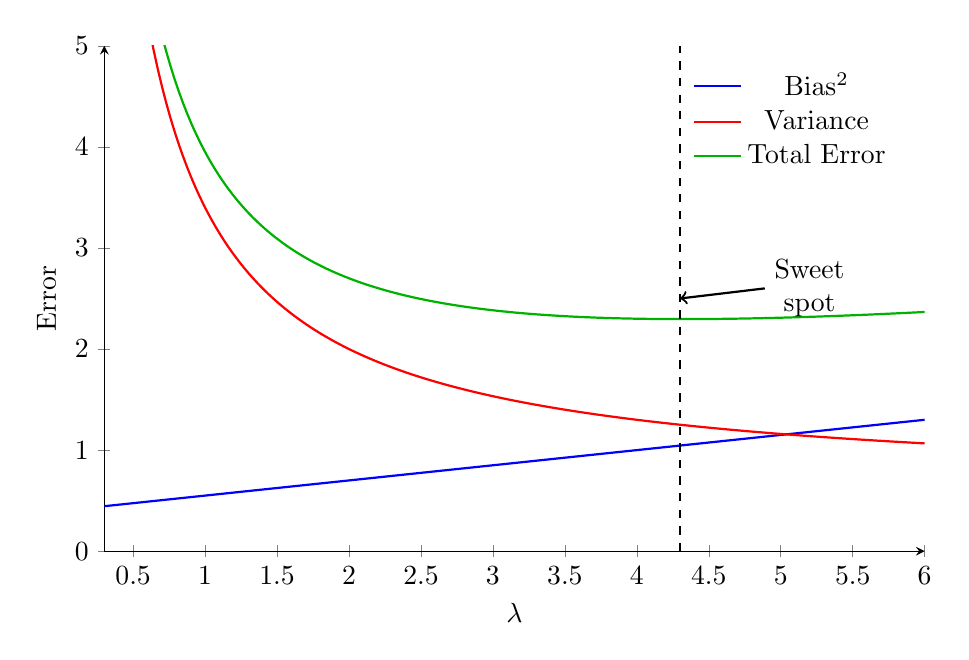
\begin{tikzpicture}
\begin{axis}[
    width=12cm,
    height=8cm,
    axis lines=left,
    xlabel={$\lambda$},
    ylabel={Error},
    xmin=0.3, xmax=6,
    ymin=0, ymax=5,
    samples=200,
    domain=0.3:6,
    legend style={draw=none, at={(0.97,0.97)}, anchor=north east}
]

\addplot[thick, blue] {0.4 + 0.15*x};
\addlegendentry{Bias$^2$}

\addplot[thick, red] {2.8/x + 0.6};
\addlegendentry{Variance}

\addplot[thick, green!70!black] {0.4 + 0.15*x + 2.8/x + 0.6};
\addlegendentry{Total Error}

\addplot[dashed] coordinates {(4.3,0) (4.3,5)};
\node[below] at (axis cs:4.3,0) {$\lambda^*$};

\node[align=center] (sweet) at (axis cs:5.2,2.6) {Sweet\\spot};
\draw[->, thick] (sweet.west) -- (axis cs:4.3,2.5);

\end{axis}
\end{tikzpicture}
\end{center}

\begin{itemize}
    \item As $\lambda$ increases: bias increases, variance decreases
    \item There exists an optimal $\lambda^*$ minimizing total error
    \item Small $\lambda$: high variance (overfitting)
    \item Large $\lambda$: high bias (underfitting)
\end{itemize}

\end{geometrybox}

\section{Choosing the Optimal $\lambda$}

\begin{importantbox}
\textbf{How do we choose $\lambda$?}

The optimal $\lambda$ depends on the data and must be chosen using \textbf{cross-validation}.

\textbf{Algorithm:}
\begin{enumerate}
    \item Choose a grid of candidate values: $\lambda \in \{0, 0.01, 0.1, 1, 10, 100, 1000\}$
    \item For each $\lambda$:
    \begin{enumerate}
        \item Use k-fold cross-validation (typically $k=5$ or $k=10$)
        \item Compute average validation error
    \end{enumerate}
    \item Select $\lambda$ with lowest validation error
    \item Refit on all training data with chosen $\lambda$
\end{enumerate}
\end{importantbox}

\subsection{Cross-Validation Procedure}

\begin{example}[5-Fold CV for Ridge]

\textbf{Setup:} 100 observations, test $\lambda \in \{0.1, 1, 10, 100\}$

\textbf{For each $\lambda$:}

\textbf{Fold 1:} Train on observations 21-100, validate on 1-20 → Error$_1(\lambda)$

\textbf{Fold 2:} Train on \{1-20, 41-100\}, validate on 21-40 → Error$_2(\lambda)$

\textbf{Fold 3:} Train on \{1-40, 61-100\}, validate on 41-60 → Error$_3(\lambda)$

\textbf{Fold 4:} Train on \{1-60, 81-100\}, validate on 61-80 → Error$_4(\lambda)$

\textbf{Fold 5:} Train on observations 1-80, validate on 81-100 → Error$_5(\lambda)$

\textbf{Average:} $\text{CV}(\lambda) = \frac{1}{5}\sum_{k=1}^{5}\text{Error}_k(\lambda)$

\textbf{Results:}
\begin{center}
\begin{tabular}{|c|c|}
\hline
$\lambda$ & CV Error \\
\hline
0.1 & 25.3 \\
1 & 22.1 \\
10 & 20.5 $\leftarrow$ \textbf{Best!} \\
100 & 23.8 \\
\hline
\end{tabular}
\end{center}

Choose $\lambda = 10$.
\end{example}

\section{Feature Scaling is CRITICAL for Ridge}

\begin{importantbox}
\textbf{MUST standardize features before ridge regression!}

Why? The penalty $\lambda \sum \beta_j^2$ treats all coefficients equally.

But if features are on different scales, this isn't fair!
\end{importantbox}

\begin{example}[Why Scaling Matters]

Suppose we predict house price using:
\begin{itemize}
    \item $x_1$: Size in sq ft (range: 1000-5000)
    \item $x_2$: Number of bedrooms (range: 1-5)
\end{itemize}

\textbf{Without scaling:}
\begin{itemize}
    \item Size varies over $\approx 4000$ units
    \item Bedrooms varies over $\approx 4$ units
\end{itemize}

To have the same effect on $y$, size needs a much smaller coefficient:
\begin{equation}
    y \approx \beta_0 + 0.1 \times \text{Size} + 50 \times \text{Bedrooms}
\end{equation}

The penalty: $\lambda[(0.1)^2 + (50)^2] = \lambda[0.01 + 2500] \approx 2500\lambda$

The penalty is almost entirely on the bedrooms coefficient, even though both might be equally important!

\textbf{After standardizing both features:}

Both have mean 0, std 1, so coefficients will be on similar scales. The penalty is now fair.
\end{example}

\begin{note}
\textbf{Standardization procedure for ridge:}
\begin{enumerate}
    \item Compute mean $\bar{x}_j$ and std $s_j$ for each feature (from training data)
    \item Transform: $x_j^{\text{std}} = \frac{x_j - \bar{x}_j}{s_j}$
    \item Fit ridge regression on standardized features
    \item To interpret, can transform coefficients back to original scale
\end{enumerate}
\end{note}

\section{Ridge Regression Path}

\begin{definition}[Ridge Path]
The \textbf{ridge path} shows how each coefficient changes as $\lambda$ varies from 0 to $\infty$.

This is useful for understanding which features are more "important" (larger coefficients that shrink more slowly).
\end{definition}

\begin{geometrybox}
\textbf{Visualizing the Ridge Path:}

\begin{center}
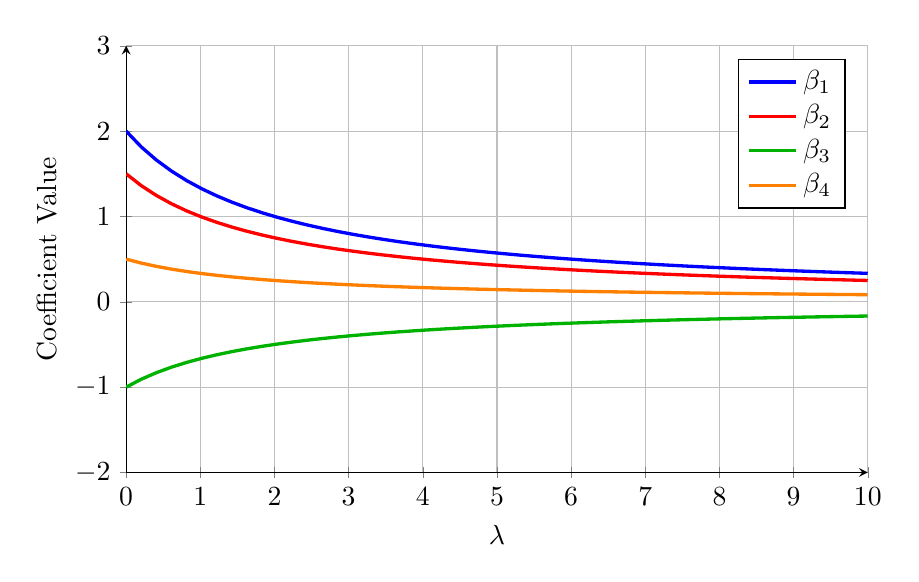
\begin{tikzpicture}[scale=1.0]
    \begin{axis}[
        axis lines = left,
        xlabel = {$\lambda$},
        ylabel = {Coefficient Value},
        xmin=0, xmax=10,
        ymin=-2, ymax=3,
        width=11cm,
        height=7cm,
        legend pos=north east,
        grid=major
    ]
    
    % Different coefficient paths
    \addplot[domain=0:10, samples=50, blue, very thick] {2/(1+0.5*x)};
    \addlegendentry{$\beta_1$}
    
    \addplot[domain=0:10, samples=50, red, very thick] {1.5/(1+0.5*x)};
    \addlegendentry{$\beta_2$}
    
    \addplot[domain=0:10, samples=50, green!70!black, very thick] {-1/(1+0.5*x)};
    \addlegendentry{$\beta_3$}
    
    \addplot[domain=0:10, samples=50, orange, very thick] {0.5/(1+0.5*x)};
    \addlegendentry{$\beta_4$}
    
    \end{axis}
\end{tikzpicture}
\end{center}

\textbf{Observations:}
\begin{itemize}
    \item All coefficients start at their OLS values ($\lambda = 0$)
    \item All shrink toward zero as $\lambda$ increases
    \item Coefficients with larger OLS values shrink more in absolute terms
    \item But all shrink at the same \textit{rate} (proportionally)
    \item None ever reach exactly zero (key difference from Lasso)
\end{itemize}
\end{geometrybox}

\section{Relationship to Constrained Optimization}

\begin{theorem}[Constrained Formulation]
Ridge regression is equivalent to:
\begin{equation}
    \min_{\boldsymbol{\beta}} \sum_{i=1}^{n}(y_i - \mathbf{x}_i^T\boldsymbol{\beta})^2 \quad \text{subject to} \quad \sum_{j=1}^{p}\beta_j^2 \leq t
\end{equation}

For every $\lambda$, there exists a $t$ that gives the same solution, and vice versa.
\end{theorem}
\pagebreak
\begin{geometrybox}
\textbf{Geometric Picture (2D case):}
\begin{center}
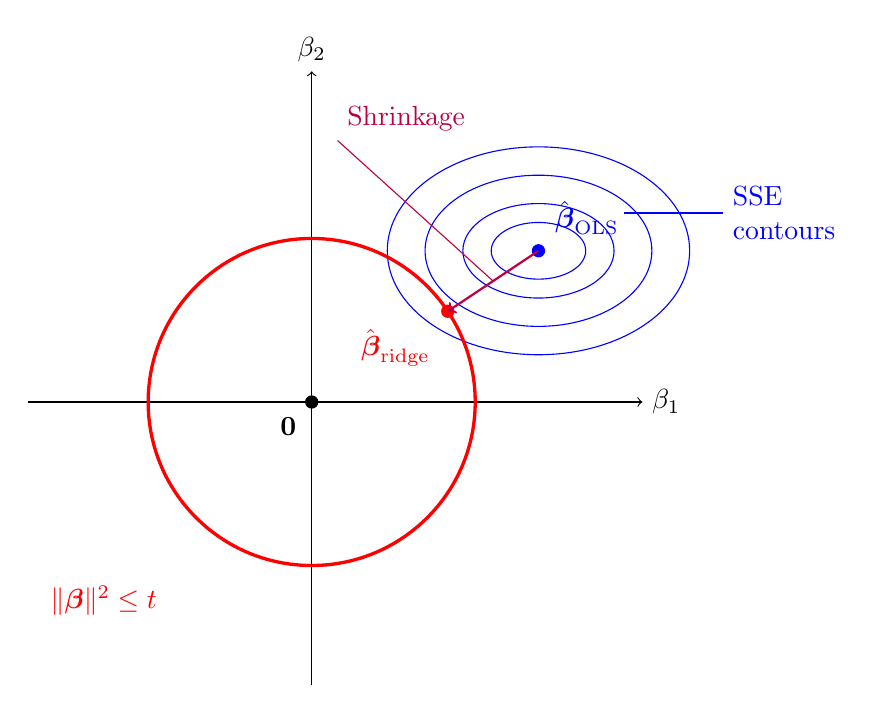
\begin{tikzpicture}[scale=1.2]

% ------------------------
% PARAMETERS
% ------------------------
\def\a{2.4}
\def\b{1.6}
\def\c{0.6}

\def\rx{\c*\a}
\def\ry{\c*\b}
\def\radius{sqrt(\rx*\rx + \ry*\ry)}

% ------------------------
% Axes
% ------------------------
\draw[->] (-3,0) -- (3.5,0) node[right] {$\beta_1$};
\draw[->] (0,-3) -- (0,3.5) node[above] {$\beta_2$};

% ------------------------
% SSE contours
% ------------------------
\foreach \x/\y in {1.6/1.1, 1.2/0.8, 0.8/0.5, 0.5/0.3}{
  \draw[blue] (\a,\b) ellipse ({\x} and {\y});
}

% Anchor point for contours (stable reference)
\coordinate (sseAnchor) at ({\a+0.9},{\b+0.4});

% SSE label (outside + pointer)
\node[blue, align=left] (sseLabel) at (5.0,2.0) {SSE\\contours};
\draw[blue, thin] (sseLabel.west) -- (sseAnchor);

% ------------------------
% Ridge constraint
% ------------------------
\draw[red, very thick] (0,0) circle (\radius);
\node[red, align=center] at (-2.2,-2.1)
  {$\|\boldsymbol{\beta}\|^2 \le t$};

% ------------------------
% Key points
% ------------------------
\fill (0,0) circle (2pt);
\node[below left=2pt] at (0,0) {$\mathbf{0}$};

\fill[blue] (\a,\b) circle (2pt);
\node[blue, above right=2.5pt] at (\a,\b)
  {$\hat{\boldsymbol{\beta}}_{\text{OLS}}$};

\fill[red] (\rx,\ry) circle (2pt);
\node[red, below left=3pt] at (\rx,\ry)
  {$\hat{\boldsymbol{\beta}}_{\text{ridge}}$};

% ------------------------
% Shrinkage (clean, non-overlapping)
% ------------------------
\draw[->, thick, purple] (\a,\b) -- (\rx,\ry);

% Shrinkage label placed in free space + connector
\node[purple] (shrinkLabel) at (1.0,3.0) {Shrinkage};
\draw[purple, thin] (shrinkLabel.south west) -- ({(\a+\rx)/2},{(\b+\ry)/2});

\end{tikzpicture}
\end{center}

\textbf{Key insights:}
\begin{itemize}
    \item Blue ellipses: contours of SSE (OLS wants the center)
    \item Red circle: ridge constraint $\beta_1^2 + \beta_2^2 \leq t$
    \item Solution: where SSE contour touches the constraint circle
    \item The constraint "pulls" the solution toward origin
    \item Ridge solution always lies on a straight line from origin through OLS solution
\end{itemize}
\end{geometrybox}

\section{Properties of Ridge Estimator}

\begin{theorem}[Properties]
    \smallskip
\begin{enumerate}
    \item \textbf{Biased:} $E[\hat{\boldsymbol{\beta}}_{\text{ridge}}] \neq \boldsymbol{\beta}_{\text{true}}$ (in general)
    
    \item \textbf{Lower variance:} $\text{Var}(\hat{\boldsymbol{\beta}}_{\text{ridge}}) < \text{Var}(\hat{\boldsymbol{\beta}}_{\text{OLS}})$
    
    \item \textbf{MSE can be lower:} Despite bias, MSE = Bias$^2$ + Variance can be lower than OLS
    
    \item \textbf{Continuous in $\lambda$:} Small changes in $\lambda$ → small changes in $\hat{\boldsymbol{\beta}}$
    
    \item \textbf{All coefficients non-zero:} No automatic feature selection
\end{enumerate}
\end{theorem}

\section{When to Use Ridge Regression}

\begin{importantbox}
\textbf{Use ridge regression when:}

\begin{enumerate}
    \item \textbf{High multicollinearity:} Predictors are highly correlated
    \item \textbf{$p > n$:} More features than observations
    \item \textbf{Many features:} High-dimensional data
    \item \textbf{Numerical instability:} OLS estimates are unstable
    \item \textbf{Regularization needed:} Want to prevent overfitting
    \item \textbf{Believe all features relevant:} Want to keep all variables (with shrinkage)
\end{enumerate}

\textbf{Don't use ridge if:}
\begin{itemize}
    \item You need feature selection (many truly irrelevant features) → Use Lasso instead
    \item No multicollinearity and $n >> p$ → OLS is fine
    \item Need exact sparsity (exactly zero coefficients) → Use Lasso
\end{itemize}
\end{importantbox}

\section{GATE-Style Problems}

\begin{example}[Problem 1: Computing Ridge Estimate]
\textbf{Given:}
\begin{equation}
    \mathbf{X}^T\mathbf{X} = \begin{bmatrix} 5 & 2 \\ 2 & 3 \end{bmatrix}, \quad
    \mathbf{X}^T\mathbf{y} = \begin{bmatrix} 10 \\ 8 \end{bmatrix}, \quad
    \lambda = 1
\end{equation}

\textbf{Find:} Ridge estimate $\hat{\boldsymbol{\beta}}_{\text{ridge}}$

\textbf{Solution:}

\textbf{Step 1:} Compute $\mathbf{X}^T\mathbf{X} + \lambda\mathbf{I}$
\begin{equation}
    \mathbf{X}^T\mathbf{X} + \mathbf{I} = \begin{bmatrix} 5 & 2 \\ 2 & 3 \end{bmatrix} + \begin{bmatrix} 1 & 0 \\ 0 & 1 \end{bmatrix} = \begin{bmatrix} 6 & 2 \\ 2 & 4 \end{bmatrix}
\end{equation}

\textbf{Step 2:} Compute inverse
\begin{equation}
    (\mathbf{X}^T\mathbf{X} + \mathbf{I})^{-1} = \frac{1}{6(4) - 2(2)}\begin{bmatrix} 4 & -2 \\ -2 & 6 \end{bmatrix} = \frac{1}{20}\begin{bmatrix} 4 & -2 \\ -2 & 6 \end{bmatrix}
\end{equation}

\textbf{Step 3:} Compute $\hat{\boldsymbol{\beta}}$
\begin{equation}
    \hat{\boldsymbol{\beta}} = \frac{1}{20}\begin{bmatrix} 4 & -2 \\ -2 & 6 \end{bmatrix}\begin{bmatrix} 10 \\ 8 \end{bmatrix} = \frac{1}{20}\begin{bmatrix} 40-16 \\ -20+48 \end{bmatrix} = \frac{1}{20}\begin{bmatrix} 24 \\ 28 \end{bmatrix} = \begin{bmatrix} 1.2 \\ 1.4 \end{bmatrix}
\end{equation}

\textbf{Answer:} $\hat{\boldsymbol{\beta}}_{\text{ridge}} = [1.2, 1.4]^T$
\end{example}

\begin{example}[Problem 2: Comparing OLS and Ridge]
\textbf{Question:} True or False?

(a) Ridge regression coefficients are always smaller in magnitude than OLS coefficients.

(b) As $\lambda \to \infty$, ridge coefficients approach zero.

(c) Ridge regression can make some coefficients exactly zero.

(d) Ridge regression always has lower MSE than OLS.

\textbf{Answers:}

(a) \textbf{True.} Ridge shrinks all coefficients toward zero.

(b) \textbf{True.} As penalty increases, all coefficients shrink toward zero (but never reach it in finite $\lambda$).

(c) \textbf{False.} Ridge shrinks coefficients but never makes them exactly zero (unlike Lasso).

(d) \textbf{False.} Ridge has lower prediction MSE than OLS for appropriate $\lambda$, but not always. If $\lambda$ is too large (too much bias) or data truly follows OLS assumptions perfectly, OLS can be better.
\end{example}

\begin{example}[Problem 3: Effect of $\lambda$]
\textbf{Given:} OLS estimate is $\hat{\boldsymbol{\beta}}_{\text{OLS}} = [3, -2, 5]^T$

\textbf{Question:} What happens to ridge estimate as $\lambda$ changes from 0 to $\infty$?

\textbf{Answer:}

At $\lambda = 0$: $\hat{\boldsymbol{\beta}}_{\text{ridge}} = [3, -2, 5]^T$ (same as OLS)

As $\lambda$ increases: All coefficients shrink toward 0 proportionally

At $\lambda = \infty$: $\hat{\boldsymbol{\beta}}_{\text{ridge}} \to [0, 0, 0]^T$

The path is continuous: [3, -2, 5] → [2.5, -1.6, 4.2] → [2, -1.3, 3.3] → ... → [0, 0, 0]
\end{example}

\section{Summary - Key Points for GATE}

\begin{importantbox}
\textbf{Must Know for GATE:}

\begin{enumerate}
    \item \textbf{Motivation:} Solves multicollinearity, $p > n$, overfitting problems
    
    \item \textbf{Objective:} Minimize $||\mathbf{y} - \mathbf{X}\boldsymbol{\beta}||^2 + \lambda||\boldsymbol{\beta}||^2$
    
    \item \textbf{Solution:} $\hat{\boldsymbol{\beta}}_{\text{ridge}} = (\mathbf{X}^T\mathbf{X} + \lambda\mathbf{I})^{-1}\mathbf{X}^T\mathbf{y}$
    
    \item \textbf{Key property:} $\mathbf{X}^T\mathbf{X} + \lambda\mathbf{I}$ always invertible for $\lambda > 0$
    
    \item \textbf{Effect of $\lambda$:}
    \begin{itemize}
        \item $\lambda = 0$: OLS
        \item $\lambda$ small: close to OLS
        \item $\lambda$ large: strong shrinkage
        \item $\lambda = \infty$: all $\beta = 0$
    \end{itemize}
    
    \item \textbf{Bias-variance:} Introduces bias, reduces variance, can lower total MSE
    
    \item \textbf{Standardization:} MUST standardize features before applying ridge
    
    \item \textbf{Feature selection:} Does NOT do feature selection (all coefficients non-zero)
    
    \item \textbf{Choosing $\lambda$:} Use cross-validation
    
    \item \textbf{Comparison with OLS:}
    \begin{itemize}
        \item More stable (lower variance)
        \item Biased
        \item Works when OLS fails ($p > n$)
    \end{itemize}
\end{enumerate}
\end{importantbox}

\begin{gatepoint}
\textbf{Common GATE Question Types:}

\begin{enumerate}
    \item Given $\mathbf{X}^T\mathbf{X}$, $\mathbf{X}^T\mathbf{y}$, and $\lambda$, compute ridge estimate
    \item Understand effect of changing $\lambda$
    \item Know when ridge fails to give solution (never! always invertible)
    \item Compare ridge vs OLS properties
    \item Understand bias-variance trade-off
    \item Know ridge doesn't do feature selection
    \item Understand why standardization is necessary
\end{enumerate}
\end{gatepoint}
\chapter{Logistic Regression: Introduction to Classification}

\section{From Regression to Classification}

\begin{mentalmodel}
So far, we've predicted \textbf{continuous} values (house prices, temperatures, etc.).

But many real-world problems involve predicting \textbf{categories}:
\begin{itemize}
    \item Will this customer buy? (Yes/No)
    \item Is this email spam? (Spam/Not Spam)
    \item Will the student pass? (Pass/Fail)
    \item Is this tumor malignant? (Malignant/Benign)
\end{itemize}

These are \textbf{classification} problems. Logistic regression is our first classification method!
\end{mentalmodel}

\subsection{Binary Classification}

\begin{definition}[Binary Classification Problem]
We have:
\begin{itemize}
    \item Input features: $\mathbf{x} = [x_1, x_2, \ldots, x_p]^T$
    \item Output: $y \in \{0, 1\}$ (two classes)
\end{itemize}

Common encodings:
\begin{itemize}
    \item Class 0: Negative class (No, Fail, Benign, Not Spam)
    \item Class 1: Positive class (Yes, Pass, Malignant, Spam)
\end{itemize}
\end{definition}

\begin{example}[Email Spam Classification]
\textbf{Features:}
\begin{itemize}
    \item $x_1$: Number of times word "free" appears
    \item $x_2$: Number of times word "money" appears
    \item $x_3$: Number of exclamation marks
    \item $x_4$: Length of email
\end{itemize}

\textbf{Output:}
\begin{itemize}
    \item $y = 1$: Spam
    \item $y = 0$: Not spam (Ham)
\end{itemize}
\end{example}

\section{Why Linear Regression Fails for Classification}

\begin{mentalmodel}
You might think: "Let's just use linear regression with $y \in \{0, 1\}$!"

This doesn't work well. Let me show you why.
\end{mentalmodel}

\begin{example}[The Problem with Linear Regression]

\textbf{Data:} Predicting if a student passes based on study hours

\begin{center}
\begin{tabular}{|c|c|}
\hline
Study Hours ($x$) & Pass ($y$) \\
\hline
1 & 0 \\
2 & 0 \\
3 & 0 \\
4 & 1 \\
5 & 1 \\
6 & 1 \\
\hline
\end{tabular}
\end{center}

\textbf{Linear regression might give:} $\hat{y} = -0.6 + 0.3x$

\textbf{Problems:}
\begin{enumerate}
    \item For $x = 0$: $\hat{y} = -0.6$ (negative probability?!)
    \item For $x = 10$: $\hat{y} = 2.4$ (probability $>$ 1?!)
    \item We need: $0 \leq \hat{y} \leq 1$ always
\end{enumerate}

\begin{center}
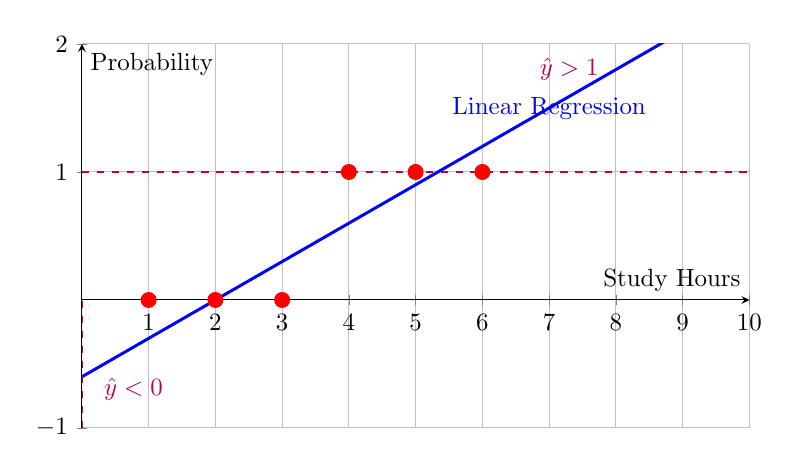
\begin{tikzpicture}[scale=0.9]
    \begin{axis}[
        axis lines = middle,
        xlabel = {Study Hours},
        ylabel = {Probability},
        xmin=0, xmax=10,
        ymin=-1, ymax=2,
        width=11cm,
        height=7cm,
        grid=major
    ]
    
    % Linear regression line
    \addplot[domain=0:10, samples=2, blue, very thick] {-0.6 + 0.3*x};
    \node[blue] at (7,1.5) {Linear Regression};
    
    % Data points
    \addplot[only marks, mark=*, mark size=3pt, red] coordinates {
        (1, 0) (2, 0) (3, 0) (4, 1) (5, 1) (6, 1)
    };
    
    % Problematic regions
    \draw[dashed, thick, purple] (0,-1) -- (0,0);
    \node[purple, right] at (0.2,-0.7) {$\hat{y} < 0$};
    
    \draw[dashed, thick, purple] (0,1) -- (10,1);
    \node[purple] at (7.3,1.8) {$\hat{y} > 1$};
    
    \end{axis}
\end{tikzpicture}
\end{center}

Linear regression doesn't respect the constraint $0 \leq P(y=1) \leq 1$!
\end{example}

\section{The Logistic Function (Sigmoid Function)}

\begin{keyidea}
We need a function that:
\begin{enumerate}
    \item Takes any real input: $z \in (-\infty, \infty)$
    \item Outputs a value in $(0, 1)$: valid probability
    \item Is smooth and differentiable (for optimization)
\end{enumerate}

The \textbf{logistic function} (also called \textbf{sigmoid function}) does exactly this!
\end{keyidea}

\begin{definition}[Logistic/Sigmoid Function]
\begin{equation}
    \sigma(z) = \frac{1}{1 + e^{-z}} = \frac{e^z}{1 + e^z}
\end{equation}

\textbf{Properties:}
\begin{enumerate}
    \item Domain: $z \in \mathbb{R}$ (any real number)
    \item Range: $\sigma(z) \in (0, 1)$ (always a valid probability)
    \item $\sigma(0) = 0.5$ (midpoint)
    \item $\sigma(-z) = 1 - \sigma(z)$ (symmetry)
    \item $\lim_{z \to \infty} \sigma(z) = 1$
    \item $\lim_{z \to -\infty} \sigma(z) = 0$
    \item Derivative: $\frac{d\sigma}{dz} = \sigma(z)(1 - \sigma(z))$ (very useful!)
\end{enumerate}
\end{definition}

\begin{example}[Computing Sigmoid Values]

\textbf{Case 1:} $z = 0$
\begin{equation}
    \sigma(0) = \frac{1}{1 + e^{0}} = \frac{1}{1 + 1} = \frac{1}{2} = 0.5
\end{equation}

\textbf{Case 2:} $z = 2$
\begin{equation}
    \sigma(2) = \frac{1}{1 + e^{-2}} = \frac{1}{1 + 0.135} = \frac{1}{1.135} \approx 0.881
\end{equation}

\textbf{Case 3:} $z = -3$
\begin{equation}
    \sigma(-3) = \frac{1}{1 + e^{3}} = \frac{1}{1 + 20.09} = \frac{1}{21.09} \approx 0.047
\end{equation}

\textbf{Case 4:} $z = 5$
\begin{equation}
    \sigma(5) = \frac{1}{1 + e^{-5}} = \frac{1}{1 + 0.0067} \approx 0.993
\end{equation}

Notice: Large positive $z$ → $\sigma(z) \approx 1$, Large negative $z$ → $\sigma(z) \approx 0$
\end{example}

\begin{geometrybox}
\textbf{Visualizing the Sigmoid Function:}

\begin{center}
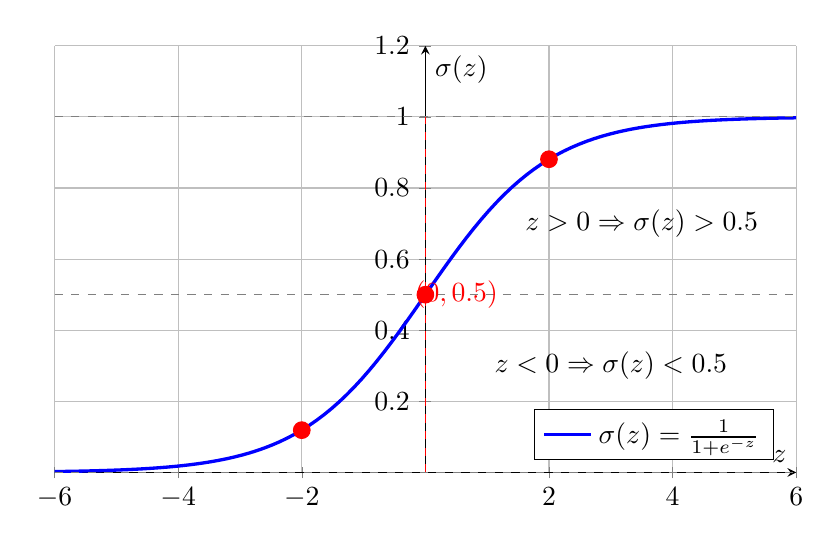
\begin{tikzpicture}[scale=1.0]
    \begin{axis}[
        axis lines = center,
        xlabel = {$z$},
        ylabel = {$\sigma(z)$},
        ymin=0, ymax=1.2,
        xmin=-6, xmax=6,
        domain=-6:6,
        samples=100,
        width=11cm,
        height=7cm,
        grid=major,
        legend pos=south east
    ]
    
    % Sigmoid curve
    \addplot[blue, very thick] {1/(1+exp(-x))};
    \addlegendentry{$\sigma(z) = \frac{1}{1+e^{-z}}$}
    
    % Horizontal lines at 0, 0.5, 1
    \addplot[dashed, gray] coordinates {(-6,0.5) (6,0.5)};
    \addplot[dashed, gray] coordinates {(-6,0) (6,0)};
    \addplot[dashed, gray] coordinates {(-6,1) (6,1)};
    
    % Vertical line at 0
    \addplot[dashed, red] coordinates {(0,0) (0,1)};
    
    % Key points
    \addplot[only marks, mark=*, mark size=3pt, red] coordinates {
        (0, 0.5) (-2, 0.119) (2, 0.881)
    };
    
    % Annotations
    \node[red] at (0.5, 0.5) {$(0, 0.5)$};
    \node at (3, 0.3) {$z < 0 \Rightarrow \sigma(z) < 0.5$};
    \node at (3.5, 0.7) {$z > 0 \Rightarrow \sigma(z) > 0.5$};
    
    \end{axis}
\end{tikzpicture}
\end{center}

\textbf{Key observations:}
\begin{itemize}
    \item S-shaped curve (hence "sigmoid" = S-shaped in Greek)
    \item Smooth transition from 0 to 1
    \item Steep change around $z = 0$
    \item Asymptotically approaches 0 and 1
\end{itemize}
\end{geometrybox}

\section{The Logistic Regression Model}

\begin{definition}[Logistic Regression Model]
We model the probability that $y = 1$ given features $\mathbf{x}$:

\begin{equation}
    P(y = 1 | \mathbf{x}) = \sigma(\beta_0 + \beta_1 x_1 + \beta_2 x_2 + \cdots + \beta_p x_p)
\end{equation}

Or more compactly, with $z = \beta_0 + \beta_1 x_1 + \cdots + \beta_p x_p = \mathbf{x}^T\boldsymbol{\beta}$:

\begin{equation}
    P(y = 1 | \mathbf{x}) = \sigma(z) = \frac{1}{1 + e^{-z}} = \frac{1}{1 + e^{-\mathbf{x}^T\boldsymbol{\beta}}}
\end{equation}

And consequently:
\begin{equation}
    P(y = 0 | \mathbf{x}) = 1 - P(y = 1 | \mathbf{x}) = 1 - \sigma(z) = \sigma(-z)
\end{equation}
\end{definition}

\begin{mentalmodel}
\textbf{Two-step process:}

\textbf{Step 1:} Compute linear combination (just like linear regression)
\begin{equation}
    z = \beta_0 + \beta_1 x_1 + \beta_2 x_2 + \cdots + \beta_p x_p
\end{equation}

\textbf{Step 2:} Pass through sigmoid to get probability
\begin{equation}
    P(y = 1) = \sigma(z) = \frac{1}{1 + e^{-z}}
\end{equation}

Think of $z$ as a "score" - high score means likely class 1, low score means likely class 0.
\end{mentalmodel}

\begin{example}[Spam Classification Model]
Suppose we fit a logistic regression:
\begin{equation}
    P(\text{Spam} | \mathbf{x}) = \sigma(-2 + 0.5 x_1 + 0.3 x_2 + 0.1 x_3)
\end{equation}

where:
\begin{itemize}
    \item $x_1$: count of word "free"
    \item $x_2$: count of word "money"  
    \item $x_3$: number of exclamation marks
\end{itemize}

\textbf{Email 1:} "free" appears 3 times, "money" once, 2 exclamation marks
\begin{align}
    z &= -2 + 0.5(3) + 0.3(1) + 0.1(2) = -2 + 1.5 + 0.3 + 0.2 = 0 \\
    P(\text{Spam}) &= \sigma(0) = 0.5
\end{align}

Uncertain! 50% chance of spam.

\textbf{Email 2:} "free" appears 10 times, "money" 5 times, 8 exclamation marks
\begin{align}
    z &= -2 + 0.5(10) + 0.3(5) + 0.1(8) = -2 + 5 + 1.5 + 0.8 = 5.3 \\
    P(\text{Spam}) &= \sigma(5.3) = \frac{1}{1 + e^{-5.3}} \approx 0.995
\end{align}

Very likely spam! (99.5% probability)

\textbf{Email 3:} "free" appears 0 times, "money" 0 times, 0 exclamation marks
\begin{align}
    z &= -2 + 0 + 0 + 0 = -2 \\
    P(\text{Spam}) &= \sigma(-2) = \frac{1}{1 + e^{2}} \approx 0.119
\end{align}

Likely not spam (only 11.9% probability).
\end{example}

\section{Decision Boundary}

\begin{definition}[Classification Rule]
Given probability $P(y = 1 | \mathbf{x})$, we classify as:
\begin{equation}
    \hat{y} = \begin{cases}
        1 & \text{if } P(y = 1 | \mathbf{x}) \geq 0.5 \\
        0 & \text{if } P(y = 1 | \mathbf{x}) < 0.5
    \end{cases}
\end{equation}

We can adjust the threshold (0.5) based on the application!
\end{definition}

\begin{theorem}[Decision Boundary]
Since $\sigma(z) = 0.5$ when $z = 0$, the decision boundary is:
\begin{equation}
    \beta_0 + \beta_1 x_1 + \beta_2 x_2 + \cdots + \beta_p x_p = 0
\end{equation}

This is a \textbf{hyperplane} in feature space!
\end{theorem}

\begin{geometrybox}
\textbf{Decision Boundary Visualization (2D):}

With two features, the boundary is a line: $\beta_0 + \beta_1 x_1 + \beta_2 x_2 = 0$

\begin{center}
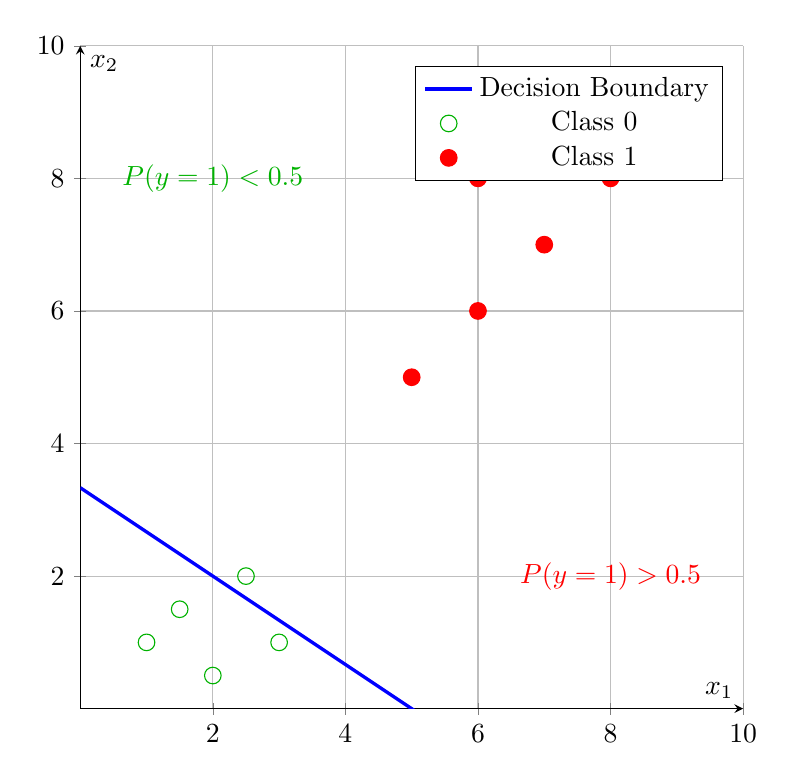
\begin{tikzpicture}[scale=1.0]
    \begin{axis}[
        axis lines = center,
        xlabel = {$x_1$},
        ylabel = {$x_2$},
        xmin=0, xmax=10,
        ymin=0, ymax=10,
        width=10cm,
        height=10cm,
        grid=major,
        legend pos=north east
    ]
    
    % Decision boundary: -2 + 0.4*x1 + 0.6*x2 = 0
    % => x2 = (2 - 0.4*x1)/0.6
    \addplot[domain=0:10, samples=2, blue, very thick] {(2 - 0.4*x)/0.6};
    \addlegendentry{Decision Boundary}
    
    % Class 0 points (below line)
    \addplot[only marks, mark=o, mark size=3pt, green!70!black] coordinates {
        (1, 1) (2, 0.5) (1.5, 1.5) (3, 1) (2.5, 2)
    };
    \addlegendentry{Class 0}
    
    % Class 1 points (above line)
    \addplot[only marks, mark=*, mark size=3pt, red] coordinates {
        (5, 5) (6, 6) (7, 7) (8, 8) (6, 8)
    };
    \addlegendentry{Class 1}
    
    % Regions
    \node[green!70!black] at (2, 8) {$P(y=1) < 0.5$};
    \node[red] at (8, 2) {$P(y=1) > 0.5$};
    
    \end{axis}
\end{tikzpicture}
\end{center}

\textbf{Points on one side:} Classified as 0

\textbf{Points on other side:} Classified as 1

\textbf{On the boundary:} $P(y=1) = 0.5$ (tie)
\end{geometrybox}

\begin{example}[Finding the Decision Boundary]
Model: $P(y = 1) = \sigma(-3 + 2x_1 + x_2)$

\textbf{Decision boundary:} Set $z = 0$
\begin{align}
    -3 + 2x_1 + x_2 &= 0 \\
    x_2 &= 3 - 2x_1
\end{align}

This is a line with slope $-2$ and y-intercept $3$.

\textbf{Classification:}
\begin{itemize}
    \item Above the line ($x_2 > 3 - 2x_1$): Predict class 1
    \item Below the line ($x_2 < 3 - 2x_1$): Predict class 0
    \item On the line: $P(y=1) = 0.5$
\end{itemize}
\end{example}

\section{The Log-Odds (Logit) Interpretation}

\begin{definition}[Odds]
If $p = P(y = 1)$, the \textbf{odds} in favor of class 1 are:
\begin{equation}
    \text{Odds} = \frac{p}{1-p} = \frac{P(y=1)}{P(y=0)}
\end{equation}
\end{definition}

\begin{example}[Understanding Odds]
\begin{itemize}
    \item If $p = 0.5$: Odds = $\frac{0.5}{0.5} = 1$ ("even odds" or "1 to 1")
    \item If $p = 0.75$: Odds = $\frac{0.75}{0.25} = 3$ ("3 to 1 in favor")
    \item If $p = 0.8$: Odds = $\frac{0.8}{0.2} = 4$ ("4 to 1 in favor")
    \item If $p = 0.9$: Odds = $\frac{0.9}{0.1} = 9$ ("9 to 1 in favor")
\end{itemize}
\end{example}

\begin{theorem}[Log-Odds are Linear!]
Starting from the logistic regression model:
\begin{equation}
    p = P(y=1|\mathbf{x}) = \frac{1}{1 + e^{-z}} = \frac{e^z}{1 + e^z}
\end{equation}

Then:
\begin{equation}
    1 - p = \frac{1}{1 + e^{z}}
\end{equation}

The odds are:
\begin{align}
    \frac{p}{1-p} &= \frac{\frac{e^z}{1+e^z}}{\frac{1}{1+e^z}} = e^z
\end{align}

Taking the natural logarithm:
\begin{equation}
    \boxed{\log\left(\frac{p}{1-p}\right) = z = \beta_0 + \beta_1 x_1 + \cdots + \beta_p x_p}
\end{equation}

This is called the \textbf{logit function} (inverse of logistic function).
\end{theorem}

\begin{keyidea}
\textbf{Beautiful insight:}

Even though the probability $p$ has a non-linear relationship with features, the \textbf{log-odds} have a perfectly \textbf{linear} relationship!

This is why it's called "logistic regression" - we're doing linear regression on the log-odds scale.
\end{keyidea}

\begin{example}[Interpreting Coefficients using Odds]
Model: $\log\left(\frac{p}{1-p}\right) = -2 + 0.5x_1 + 0.3x_2$

\textbf{Question:} What happens to odds when $x_1$ increases by 1 unit?

\textbf{Answer:}
\begin{align}
    \text{New log-odds} &= -2 + 0.5(x_1 + 1) + 0.3x_2 \\
    &= (-2 + 0.5x_1 + 0.3x_2) + 0.5 \\
    &= \text{Old log-odds} + 0.5
\end{align}

Taking exponentials:
\begin{equation}
    \text{New odds} = e^{\text{Old log-odds} + 0.5} = e^{\text{Old log-odds}} \times e^{0.5} = \text{Old odds} \times 1.65
\end{equation}

\textbf{Interpretation:} A one-unit increase in $x_1$ \textbf{multiplies the odds by} $e^{0.5} \approx 1.65$ (or increases odds by 65\%).
\end{example}

\section{Maximum Likelihood Estimation}

\begin{mentalmodel}
Unlike linear regression (where we used least squares), for logistic regression we use \textbf{Maximum Likelihood Estimation (MLE)}.

The idea: Find parameters $\boldsymbol{\beta}$ that make the observed data most probable.
\end{mentalmodel}

\subsection{The Likelihood Function}

\begin{definition}[Likelihood for Single Observation]
For observation $(\mathbf{x}_i, y_i)$ where $y_i \in \{0, 1\}$:

Let $p_i = P(y_i = 1|\mathbf{x}_i) = \sigma(\mathbf{x}_i^T\boldsymbol{\beta})$

The probability of observing $y_i$ is:
\begin{equation}
    P(y_i | \mathbf{x}_i, \boldsymbol{\beta}) = p_i^{y_i}(1-p_i)^{1-y_i}
\end{equation}

\textbf{Why this works:}
\begin{itemize}
    \item If $y_i = 1$: $P = p_i^1(1-p_i)^0 = p_i$ (correct!)
    \item If $y_i = 0$: $P = p_i^0(1-p_i)^1 = 1-p_i$ (correct!)
\end{itemize}
\end{definition}

\begin{definition}[Likelihood for All Data]
Assuming observations are independent:
\begin{equation}
    L(\boldsymbol{\beta}) = \prod_{i=1}^{n} P(y_i | \mathbf{x}_i, \boldsymbol{\beta}) = \prod_{i=1}^{n} p_i^{y_i}(1-p_i)^{1-y_i}
\end{equation}

\textbf{Goal:} Maximize $L(\boldsymbol{\beta})$ with respect to $\boldsymbol{\beta}$.
\end{definition}

\subsection{Log-Likelihood}

\begin{keyidea}
Products are hard to work with! Take logarithm (monotonic transformation preserves maximum):
\begin{align}
    \ell(\boldsymbol{\beta}) &= \log L(\boldsymbol{\beta}) \\
    &= \sum_{i=1}^{n} \log[p_i^{y_i}(1-p_i)^{1-y_i}] \\
    &= \sum_{i=1}^{n} [y_i \log p_i + (1-y_i)\log(1-p_i)]
\end{align}

This is the \textbf{log-likelihood function}.

\textbf{Goal:} Maximize $\ell(\boldsymbol{\beta})$ (equivalent to maximizing $L(\boldsymbol{\beta})$).
\end{keyidea}

\begin{definition}[Cross-Entropy Loss]
It's common to \textbf{minimize the negative log-likelihood}:
\begin{equation}
    J(\boldsymbol{\beta}) = -\ell(\boldsymbol{\beta}) = -\sum_{i=1}^{n} [y_i \log p_i + (1-y_i)\log(1-p_i)]
\end{equation}

This is called the \textbf{cross-entropy loss} or \textbf{log loss}.

Substituting $p_i = \sigma(z_i)$ where $z_i = \mathbf{x}_i^T\boldsymbol{\beta}$:
\begin{equation}
    J(\boldsymbol{\beta}) = \sum_{i=1}^{n} \left[\log(1 + e^{z_i}) - y_i z_i\right]
\end{equation}
\end{definition}

\section{No Closed-Form Solution: Gradient Descent}

\begin{importantbox}
\textbf{Key Difference from Linear Regression:}

Linear regression has a closed-form solution: $\hat{\boldsymbol{\beta}} = (\mathbf{X}^T\mathbf{X})^{-1}\mathbf{X}^T\mathbf{y}$

Logistic regression has \textbf{NO closed-form solution}! We must use iterative optimization.

Most common method: \textbf{Gradient Descent}
\end{importantbox}

\subsection{Computing the Gradient}

\begin{theorem}[Gradient of Log-Likelihood]
The gradient of $J(\boldsymbol{\beta})$ with respect to $\boldsymbol{\beta}$ is:
\begin{equation}
    \nabla J(\boldsymbol{\beta}) = \sum_{i=1}^{n} (p_i - y_i)\mathbf{x}_i = \mathbf{X}^T(\mathbf{p} - \mathbf{y})
\end{equation}

where $p_i = \sigma(\mathbf{x}_i^T\boldsymbol{\beta})$ and $\mathbf{p} = [p_1, p_2, \ldots, p_n]^T$.
\end{theorem}

\begin{proof}[Derivation for single parameter]
For parameter $\beta_j$:
\begin{align}
    \frac{\partial J}{\partial \beta_j} &= \sum_{i=1}^{n} \frac{\partial}{\partial \beta_j}\left[\log(1+e^{z_i}) - y_i z_i\right] \\
    &= \sum_{i=1}^{n} \left[\frac{e^{z_i}}{1+e^{z_i}} \cdot x_{ij} - y_i x_{ij}\right] \\
    &= \sum_{i=1}^{n} \left[\sigma(z_i) - y_i\right]x_{ij} \\
    &= \sum_{i=1}^{n} (p_i - y_i)x_{ij}
\end{align}

In matrix form: $\nabla J = \mathbf{X}^T(\mathbf{p} - \mathbf{y})$
\end{proof}

\begin{mentalmodel}
\textbf{Beautiful observation:}

The gradient has the same form as linear regression!
\begin{equation}
    \nabla J = \mathbf{X}^T(\text{predictions} - \text{actual})
\end{equation}

The only difference: predictions come from $\sigma(z)$ instead of $z$ directly.
\end{mentalmodel}

\subsection{Gradient Descent Algorithm}

\begin{definition}[Gradient Descent for Logistic Regression]
\textbf{Initialize:} $\boldsymbol{\beta}^{(0)} = \mathbf{0}$ (or random small values)

\textbf{Repeat until convergence:}
\begin{equation}
    \boldsymbol{\beta}^{(t+1)} = \boldsymbol{\beta}^{(t)} - \alpha \nabla J(\boldsymbol{\beta}^{(t)})
\end{equation}

where:
\begin{itemize}
    \item $\alpha > 0$ is the \textbf{learning rate} (step size)
    \item $\nabla J(\boldsymbol{\beta}^{(t)}) = \mathbf{X}^T(\mathbf{p}^{(t)} - \mathbf{y})$
    \item $\mathbf{p}^{(t)}$ are predictions at iteration $t$
\end{itemize}

\textbf{Convergence:} Stop when $||\nabla J|| < \epsilon$ or $||boldsymbol{\beta}^{(t+1)} - \boldsymbol{\beta}^{(t)}|| < \epsilon$
\end{definition}

\begin{mentalmodel}
\textbf{Gradient descent intuition:}

Imagine you're on a hilly landscape (the loss function) trying to reach the lowest valley.

\begin{enumerate}
    \item Look at the slope where you're standing ($\nabla J$)
    \item The gradient points \textbf{uphill} (direction of steepest ascent)
    \item So move in the \textbf{opposite direction} ($-\nabla J$) to go downhill
    \item Take a step of size $\alpha$ (learning rate)
    \item Repeat until you reach the bottom (or close enough)
\end{enumerate}
\end{mentalmodel}

\section{Complete Numerical Example}

\begin{example}[Logistic Regression by Hand]

\textbf{Data:} Simple 4-point dataset

\begin{center}
\begin{tabular}{|c|c|c|}
\hline
$i$ & $x$ & $y$ \\
\hline
1 & 1 & 0 \\
2 & 2 & 0 \\
3 & 3 & 1 \\
4 & 4 & 1 \\
\hline
\end{tabular}
\end{center}

Model: $P(y=1|x) = \sigma(\beta_0 + \beta_1 x)$

Let's do a few iterations of gradient descent by hand with $\alpha = 0.1$.

\textbf{ITERATION 0: Initialize}
\begin{equation}
    \boldsymbol{\beta}^{(0)} = \begin{bmatrix} 0 \\ 0 \end{bmatrix}
\end{equation}

\textbf{ITERATION 1:}

\textbf{Step 1:} Compute $z_i = \beta_0 + \beta_1 x_i$
\begin{align}
    z_1 &= 0 + 0(1) = 0 \\
    z_2 &= 0 + 0(2) = 0 \\
    z_3 &= 0 + 0(3) = 0 \\
    z_4 &= 0 + 0(4) = 0
\end{align}

\textbf{Step 2:} Compute $p_i = \sigma(z_i) = \frac{1}{1+e^{-z_i}}$
\begin{equation}
    p_1 = p_2 = p_3 = p_4 = \frac{1}{1+e^{0}} = 0.5
\end{equation}

\textbf{Step 3:} Compute gradients
\begin{align}
    \frac{\partial J}{\partial \beta_0} &= \sum_{i=1}^{4}(p_i - y_i)(1) \\
    &= (0.5 - 0) + (0.5 - 0) + (0.5 - 1) + (0.5 - 1) \\
    &= 0.5 + 0.5 - 0.5 - 0.5 = 0
\end{align}

\begin{align}
    \frac{\partial J}{\partial \beta_1} &= \sum_{i=1}^{4}(p_i - y_i)x_i \\
    &= (0.5 - 0)(1) + (0.5 - 0)(2) + (0.5 - 1)(3) + (0.5 - 1)(4) \\
    &= 0.5 + 1.0 - 1.5 - 2.0 = -2.0
\end{align}

\textbf{Step 4:} Update parameters
\begin{align}
    \beta_0^{(1)} &= 0 - 0.1(0) = 0 \\
    \beta_1^{(1)} &= 0 - 0.1(-2.0) = 0.2
\end{align}

\textbf{ITERATION 2:}

\textbf{Step 1:} Compute new $z_i = 0 + 0.2x_i$
\begin{align}
    z_1 &= 0.2, \quad z_2 = 0.4, \quad z_3 = 0.6, \quad z_4 = 0.8
\end{align}

\textbf{Step 2:} Compute new $p_i = \sigma(z_i)$
\begin{align}
    p_1 &= \frac{1}{1+e^{-0.2}} \approx 0.550 \\
    p_2 &= \frac{1}{1+e^{-0.4}} \approx 0.599 \\
    p_3 &= \frac{1}{1+e^{-0.6}} \approx 0.646 \\
    p_4 &= \frac{1}{1+e^{-0.8}} \approx 0.689
\end{align}

\textbf{Step 3:} Compute gradients
\begin{align}
    \frac{\partial J}{\partial \beta_0} &= (0.550 - 0) + (0.599 - 0) + (0.646 - 1) + (0.689 - 1) \\
    &\approx 0.484
\end{align}

\begin{align}
    \frac{\partial J}{\partial \beta_1} &= 0.550(1) + 0.599(2) + (0.646-1)(3) + (0.689-1)(4) \\
    &\approx 0.550 + 1.198 - 1.062 - 1.244 = -0.558
\end{align}

\textbf{Step 4:} Update
\begin{align}
    \beta_0^{(2)} &= 0 - 0.1(0.484) \approx -0.048 \\
    \beta_1^{(2)} &= 0.2 - 0.1(-0.558) \approx 0.256
\end{align}

\textbf{Continue for many more iterations...}

After convergence (say, 1000 iterations), we might get:
\begin{equation}
    \boldsymbol{\beta} \approx \begin{bmatrix} -3.5 \\ 1.5 \end{bmatrix}
\end{equation}

\textbf{Final Model:}
\begin{equation}
    P(y=1|x) = \sigma(-3.5 + 1.5x)
\end{equation}

\textbf{Making Predictions:}

For $x = 2.5$:
\begin{align}
    z &= -3.5 + 1.5(2.5) = 0.25 \\
    P(y=1) &= \sigma(0.25) = \frac{1}{1+e^{-0.25}} \approx 0.562
\end{align}

Since $0.562 > 0.5$, we predict $\hat{y} = 1$.

\textbf{Decision Boundary:}
\begin{align}
    -3.5 + 1.5x &= 0 \\
    x &= \frac{3.5}{1.5} \approx 2.33
\end{align}

For $x < 2.33$: predict 0. For $x > 2.33$: predict 1.
\end{example}

\section{Model Evaluation Metrics}

\subsection{Confusion Matrix}

\begin{definition}[Confusion Matrix]
For binary classification:

\begin{center}
\begin{tabular}{|c|c|c|}
\hline
 & \textbf{Predicted 0} & \textbf{Predicted 1} \\
\hline
\textbf{Actual 0} & True Negative (TN) & False Positive (FP) \\
\hline
\textbf{Actual 1} & False Negative (FN) & True Positive (TP) \\
\hline
\end{tabular}
\end{center}

\begin{itemize}
    \item \textbf{True Positive (TP):} Correctly predicted positive
    \item \textbf{True Negative (TN):} Correctly predicted negative
    \item \textbf{False Positive (FP):} Predicted positive, actually negative (Type I error)
    \item \textbf{False Negative (FN):} Predicted negative, actually positive (Type II error)
\end{itemize}
\end{definition}

\begin{example}[Spam Classification Confusion Matrix]
Out of 100 emails:
\begin{itemize}
    \item 40 actual spam, 60 actual ham
    \item Model correctly identifies 35 spam (TP)
    \item Model incorrectly marks 5 ham as spam (FP)
    \item Model misses 5 spam, calling them ham (FN)
    \item Model correctly identifies 55 ham (TN)
\end{itemize}

\begin{center}
\begin{tabular}{|c|c|c|c|}
\hline
 & \textbf{Predicted Ham} & \textbf{Predicted Spam} & \textbf{Total} \\
\hline
\textbf{Actual Ham} & TN = 55 & FP = 5 & 60 \\
\hline
\textbf{Actual Spam} & FN = 5 & TP = 35 & 40 \\
\hline
\textbf{Total} & 60 & 40 & 100 \\
\hline
\end{tabular}
\end{center}
\end{example}

\subsection{Performance Metrics}

\begin{definition}[Common Classification Metrics]

\textbf{1. Accuracy:}
\begin{equation}
    \text{Accuracy} = \frac{TP + TN}{TP + TN + FP + FN} = \frac{\text{Correct predictions}}{\text{Total predictions}}
\end{equation}

\textbf{2. Precision (Positive Predictive Value):}
\begin{equation}
    \text{Precision} = \frac{TP}{TP + FP} = \frac{\text{True positives}}{\text{Predicted positives}}
\end{equation}

"Of all we predicted positive, how many were actually positive?"

\textbf{3. Recall (Sensitivity, True Positive Rate):}
\begin{equation}
    \text{Recall} = \frac{TP}{TP + FN} = \frac{\text{True positives}}{\text{Actual positives}}
\end{equation}

"Of all actual positives, how many did we find?"

\textbf{4. Specificity (True Negative Rate):}
\begin{equation}
    \text{Specificity} = \frac{TN}{TN + FP} = \frac{\text{True negatives}}{\text{Actual negatives}}
\end{equation}

\textbf{5. F1-Score (Harmonic mean of Precision and Recall):}
\begin{equation}
    F_1 = 2 \cdot \frac{\text{Precision} \times \text{Recall}}{\text{Precision} + \text{Recall}} = \frac{2TP}{2TP + FP + FN}
\end{equation}
\end{definition}

\begin{example}[Computing Metrics]
From our spam example: TP=35, TN=55, FP=5, FN=5

\textbf{Accuracy:}
\begin{equation}
    \frac{35 + 55}{100} = \frac{90}{100} = 0.90 = 90\%
\end{equation}

\textbf{Precision:}
\begin{equation}
    \frac{35}{35 + 5} = \frac{35}{40} = 0.875 = 87.5\%
\end{equation}

\textbf{Recall:}
\begin{equation}
    \frac{35}{35 + 5} = \frac{35}{40} = 0.875 = 87.5\%
\end{equation}

\textbf{F1-Score:}
\begin{equation}
    2 \cdot \frac{0.875 \times 0.875}{0.875 + 0.875} = \frac{2 \times 0.765625}{1.75} = 0.875 = 87.5\%
\end{equation}
\end{example}

\begin{mentalmodel}
\textbf{When to use which metric?}

\textbf{Accuracy:} Good when classes are balanced. Misleading when imbalanced!

Example: 95\% of emails are ham. A model that always predicts "ham" has 95\% accuracy but is useless!

\textbf{Precision:} "When I predict positive, how often am I right?"
Use when \textbf{false positives are costly}.
Example: Spam filter - don't want to mark important emails as spam!

\textbf{Recall:} "Of all actual positives, how many did I catch?"
Use when \textbf{false negatives are costly}.
Example: Disease detection - don't want to miss sick patients!

\textbf{F1-Score:} Balance between precision and recall. Good for imbalanced classes.
\end{mentalmodel}

\subsection{ROC Curve and AUC}

\begin{definition}[ROC Curve]
The \textbf{Receiver Operating Characteristic (ROC)} curve plots:
\begin{itemize}
    \item X-axis: False Positive Rate (FPR) = $\frac{FP}{FP + TN} = 1 - \text{Specificity}$
    \item Y-axis: True Positive Rate (TPR) = $\frac{TP}{TP + FN} = \text{Recall}$
\end{itemize}

Created by varying the classification threshold from 0 to 1.

\textbf{AUC (Area Under Curve):}
\begin{itemize}
    \item AUC = 1: Perfect classifier
    \item AUC = 0.5: Random guessing (no better than coin flip)
    \item AUC < 0.5: Worse than random (predictions are backwards!)
\end{itemize}
\end{definition}
\pagebreak
\begin{geometrybox}
\textbf{ROC Curve Visualization:}

\begin{center}
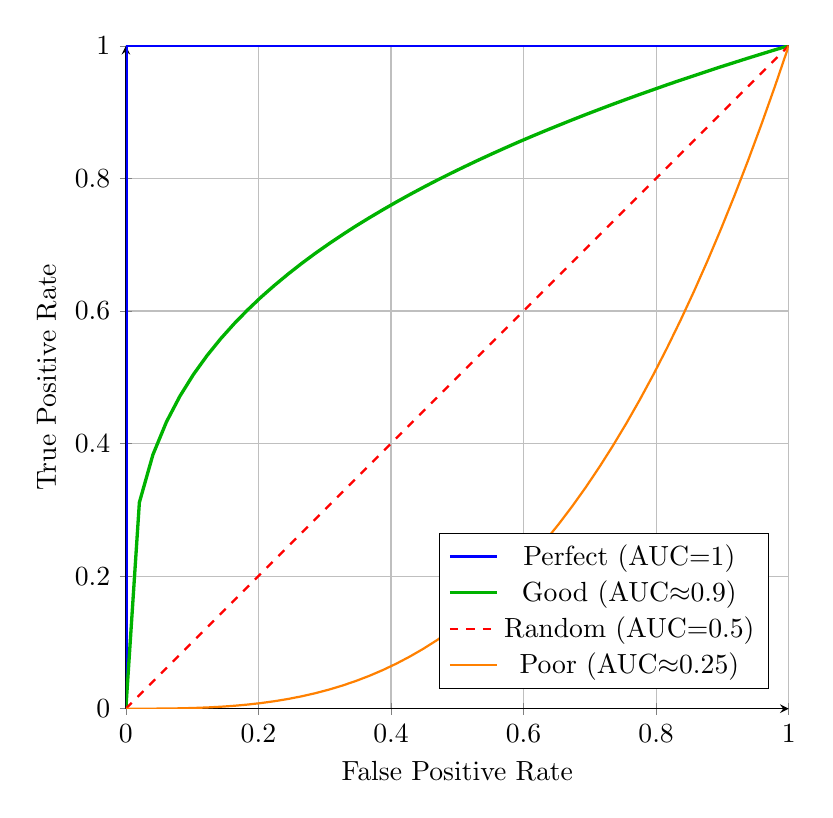
\begin{tikzpicture}[scale=1.0]
    \begin{axis}[
        axis lines = left,
        xlabel = {False Positive Rate},
        ylabel = {True Positive Rate},
        xmin=0, xmax=1,
        ymin=0, ymax=1,
        width=10cm,
        height=10cm,
        grid=major,
        legend pos=south east
    ]
    
    % Perfect classifier
    \addplot[blue, very thick] coordinates {(0,0) (0,1) (1,1)};
    \addlegendentry{Perfect (AUC=1)}
    
    % Good classifier
    \addplot[green!70!black, very thick, domain=0:1, samples=50] {x^0.3};
    \addlegendentry{Good (AUC$\approx$0.9)}
    
    % Random classifier
    \addplot[red, thick, dashed] coordinates {(0,0) (1,1)};
    \addlegendentry{Random (AUC=0.5)}
    
    % Poor classifier
    \addplot[orange, thick, domain=0:1, samples=50] {x^3};
    \addlegendentry{Poor (AUC$\approx$0.25)}
    
    \end{axis}
\end{tikzpicture}
\end{center}

\textbf{Interpretation:}
\begin{itemize}
    \item Closer to top-left corner = better classifier
    \item Diagonal line = random guessing
    \item Below diagonal = worse than random (flip predictions!)
\end{itemize}
\end{geometrybox}

\section{Multiclass Logistic Regression (Softmax)}

\begin{definition}[Softmax Regression]
For $K > 2$ classes, we generalize logistic regression using \textbf{softmax function}:

For class $k = 1, 2, \ldots, K$:
\begin{equation}
    P(y = k | \mathbf{x}) = \frac{e^{\mathbf{x}^T\boldsymbol{\beta}_k}}{\sum_{j=1}^{K} e^{\mathbf{x}^T\boldsymbol{\beta}_j}}
\end{equation}

where each class $k$ has its own coefficient vector $\boldsymbol{\beta}_k$.

\textbf{Properties:}
\begin{itemize}
    \item $P(y=k|\mathbf{x}) \in (0, 1)$ for all $k$
    \item $\sum_{k=1}^{K} P(y=k|\mathbf{x}) = 1$ (probabilities sum to 1)
\end{itemize}
\end{definition}

\begin{example}[3-Class Classification]
Classify images as: Dog, Cat, or Bird ($K=3$)

Each class has coefficients: $\boldsymbol{\beta}_{\text{dog}}, \boldsymbol{\beta}_{\text{cat}}, \boldsymbol{\beta}_{\text{bird}}$

For a new image $\mathbf{x}$:
\begin{align}
    P(\text{Dog}|\mathbf{x}) &= \frac{e^{\mathbf{x}^T\boldsymbol{\beta}_{\text{dog}}}}{e^{\mathbf{x}^T\boldsymbol{\beta}_{\text{dog}}} + e^{\mathbf{x}^T\boldsymbol{\beta}_{\text{cat}}} + e^{\mathbf{x}^T\boldsymbol{\beta}_{\text{bird}}}} \\
    P(\text{Cat}|\mathbf{x}) &= \frac{e^{\mathbf{x}^T\boldsymbol{\beta}_{\text{cat}}}}{e^{\mathbf{x}^T\boldsymbol{\beta}_{\text{dog}}} + e^{\mathbf{x}^T\boldsymbol{\beta}_{\text{cat}}} + e^{\mathbf{x}^T\boldsymbol{\beta}_{\text{bird}}}} \\
    P(\text{Bird}|\mathbf{x}) &= \frac{e^{\mathbf{x}^T\boldsymbol{\beta}_{\text{bird}}}}{e^{\mathbf{x}^T\boldsymbol{\beta}_{\text{dog}}} + e^{\mathbf{x}^T\boldsymbol{\beta}_{\text{cat}}} + e^{\mathbf{x}^T\boldsymbol{\beta}_{\text{bird}}}}
\end{align}

Predict class with highest probability.
\end{example}

\section{GATE-Style Problems}

\begin{example}[Problem 1: Computing Sigmoid]
\textbf{Compute:} $\sigma(z)$ for $z = 0, 1, -1, 2, -2$

\textbf{Solution:}
\begin{align}
    \sigma(0) &= \frac{1}{1+e^{0}} = 0.5 \\
    \sigma(1) &= \frac{1}{1+e^{-1}} = \frac{1}{1.368} \approx 0.731 \\
    \sigma(-1) &= \frac{1}{1+e^{1}} = \frac{1}{2.718} \approx 0.268 \\
    \sigma(2) &= \frac{1}{1+e^{-2}} \approx 0.881 \\
    \sigma(-2) &= \frac{1}{1+e^{2}} \approx 0.119
\end{align}

Note: $\sigma(-z) = 1 - \sigma(z)$
\end{example}

\begin{example}[Problem 2: Decision Boundary]
\textbf{Given:} $P(y=1) = \sigma(2 - 3x_1 + 4x_2)$

\textbf{Find:} The decision boundary equation.

\textbf{Solution:}

Decision boundary where $P(y=1) = 0.5$, which occurs when:
\begin{align}
    2 - 3x_1 + 4x_2 &= 0 \\
    4x_2 &= 3x_1 - 2 \\
    x_2 &= \frac{3x_1 - 2}{4} = 0.75x_1 - 0.5
\end{align}

This is a line with slope 0.75 and y-intercept -0.5.
\end{example}

\begin{example}[Problem 3: Confusion Matrix Metrics]
\textbf{Given confusion matrix:}

\begin{center}
\begin{tabular}{|c|c|c|}
\hline
 & Predicted 0 & Predicted 1 \\
\hline
Actual 0 & 80 & 20 \\
Actual 1 & 10 & 90 \\
\hline
\end{tabular}
\end{center}

\textbf{Compute:} Accuracy, Precision, Recall, F1-Score

\textbf{Solution:}

TP = 90, TN = 80, FP = 20, FN = 10

\begin{align}
    \text{Accuracy} &= \frac{80+90}{200} = \frac{170}{200} = 0.85 \\
    \text{Precision} &= \frac{90}{90+20} = \frac{90}{110} \approx 0.818 \\
    \text{Recall} &= \frac{90}{90+10} = \frac{90}{100} = 0.90 \\
    F_1 &= 2 \cdot \frac{0.818 \times 0.90}{0.818 + 0.90} = \frac{1.4724}{1.718} \approx 0.857
\end{align}
\end{example}

\begin{example}[Problem 4: Odds Interpretation]
\textbf{Given:} Logistic regression with $\beta_1 = 0.8$

\textbf{Question:} If $x_1$ increases by 1, how do the odds change?

\textbf{Solution:}

The odds multiply by $e^{\beta_1} = e^{0.8} \approx 2.23$

Interpretation: A one-unit increase in $x_1$ increases the odds by 123% (more than doubles).
\end{example}

\section{Summary - Key Points for GATE}

\begin{importantbox}
\textbf{Must Know for GATE:}

\begin{enumerate}
    \item \textbf{Binary classification:} $y \in \{0, 1\}$
    
    \item \textbf{Sigmoid function:} $\sigma(z) = \frac{1}{1+e^{-z}}$, outputs probability in $(0,1)$
    
    \item \textbf{Model:} $P(y=1|\mathbf{x}) = \sigma(\beta_0 + \beta_1 x_1 + \cdots + \beta_p x_p)$
    
    \item \textbf{Decision boundary:} Hyperplane where $\beta_0 + \beta_1 x_1 + \cdots + \beta_p x_p = 0$
    
    \item \textbf{Log-odds are linear:} $\log\frac{p}{1-p} = \beta_0 + \beta_1 x_1 + \cdots + \beta_p x_p$
    
    \item \textbf{Coefficient interpretation:} $e^{\beta_j}$ = multiplicative effect on odds
    
    \item \textbf{Estimation:} Maximum Likelihood via gradient descent (no closed form!)
    
    \item \textbf{Loss function:} Cross-entropy/log-loss
    
    \item \textbf{Gradient:} $\nabla J = \mathbf{X}^T(\mathbf{p} - \mathbf{y})$
    
    \item \textbf{Confusion Matrix:} TP, TN, FP, FN
    
    \item \textbf{Metrics:}
    \begin{itemize}
        \item Accuracy = $\frac{TP+TN}{Total}$
        \item Precision = $\frac{TP}{TP+FP}$
        \item Recall = $\frac{TP}{TP+FN}$
        \item F1 = $\frac{2TP}{2TP+FP+FN}$
    \end{itemize}
    
    \item \textbf{ROC-AUC:} Measure of classifier quality (AUC=1 perfect, AUC=0.5 random)
    
    \item \textbf{Multiclass:} Softmax regression with $K$ coefficient vectors
\end{enumerate}
\end{importantbox}

\begin{gatepoint}
\textbf{Common GATE Question Types:}

\begin{enumerate}
    \item Calculate sigmoid values
    \item Find decision boundary equation
    \item Interpret coefficients using odds ratios
    \item Compute confusion matrix metrics (accuracy, precision, recall, F1)
    \item Understand when to use which metric
    \item Compare logistic vs linear regression
    \item Know gradient descent is needed (no closed form)
    \item Understand log-likelihood/cross-entropy
    \item Apply softmax for multiclass problems
\end{enumerate}
\end{gatepoint}
\chapter{k-Nearest Neighbors (k-NN): Instance-Based Learning}

\section{Introduction to k-NN}

\begin{mentalmodel}
Imagine you just moved to a new neighborhood and want to know if it's safe. What would you do?

You'd probably ask your neighbors! If most nearby neighbors say "yes, it's safe," you'd conclude it's safe. If most say "it's dangerous," you'd be cautious.

\textbf{This is exactly how k-NN works!}

"You are the average of the k people closest to you."
\end{mentalmodel}

\begin{keyidea}
k-Nearest Neighbors is fundamentally different from the methods we've seen:

\textbf{Linear/Logistic Regression:}
\begin{itemize}
    \item Learn parameters $\boldsymbol{\beta}$ from training data
    \item Throw away training data after learning
    \item Use only $\boldsymbol{\beta}$ for predictions
\end{itemize}

\textbf{k-NN:}
\begin{itemize}
    \item \textbf{No training phase!} (or "lazy learning")
    \item Keep \textbf{all training data} in memory
    \item Make predictions by looking at nearby training examples
\end{itemize}

This is called \textbf{instance-based learning} or \textbf{memory-based learning}.
\end{keyidea}

\subsection{The k-NN Algorithm}

\begin{definition}[k-Nearest Neighbors Algorithm]

\textbf{Given:}
\begin{itemize}
    \item Training data: $\{(\mathbf{x}_1, y_1), (\mathbf{x}_2, y_2), \ldots, (\mathbf{x}_n, y_n)\}$
    \item A new point $\mathbf{x}_{\text{new}}$ to classify/predict
    \item A value $k$ (number of neighbors to consider)
\end{itemize}

\textbf{Algorithm:}
\begin{enumerate}
    \item \textbf{Compute distances} from $\mathbf{x}_{\text{new}}$ to all training points
    \item \textbf{Find the $k$ closest} training points (the "neighbors")
    \item \textbf{For Classification:} Take majority vote among the $k$ neighbors
    \item \textbf{For Regression:} Take average of the $k$ neighbors' values
\end{enumerate}
\end{definition}

\begin{example}[Simple k-NN Classification]

\textbf{Training data:} 6 houses with features and classifications

\begin{center}
\begin{tabular}{|c|c|c|c|}
\hline
House & Size (sq ft) & Age (years) & Expensive? \\
\hline
A & 1500 & 5 & No \\
B & 1600 & 8 & No \\
C & 1400 & 3 & No \\
D & 2500 & 4 & Yes \\
E & 2600 & 6 & Yes \\
F & 2400 & 5 & Yes \\
\hline
\end{tabular}
\end{center}

\textbf{New house:} Size = 2000, Age = 5. Is it expensive?

Let's use $k = 3$ (consider 3 nearest neighbors).

\textbf{Step 1: Compute distances} (we'll use Euclidean distance later, but for now, visually)

\textbf{Step 2: Find 3 nearest neighbors}

Suppose after computing distances, the 3 closest are: B, D, E

\textbf{Step 3: Majority vote}
\begin{itemize}
    \item B: No (not expensive)
    \item D: Yes (expensive)
    \item E: Yes (expensive)
\end{itemize}

Vote: 2 "Yes" vs 1 "No"

\textbf{Prediction: Expensive!}
\end{example}

\section{Distance Metrics}

\begin{importantbox}
The heart of k-NN is measuring "closeness" or "similarity" between points.

We need a \textbf{distance metric} (or \textbf{similarity measure}).
\end{importantbox}

\subsection{Euclidean Distance (Most Common)}

\begin{definition}[Euclidean Distance]
For two points $\mathbf{x} = [x_1, x_2, \ldots, x_p]^T$ and $\mathbf{z} = [z_1, z_2, \ldots, z_p]^T$:

\begin{equation}
    d(\mathbf{x}, \mathbf{z}) = \sqrt{\sum_{j=1}^{p}(x_j - z_j)^2} = \sqrt{(x_1-z_1)^2 + (x_2-z_2)^2 + \cdots + (x_p-z_p)^2}
\end{equation}

This is the ordinary "straight-line" distance.
\end{definition}

\begin{example}[Computing Euclidean Distance]

\textbf{Point 1:} $\mathbf{x} = [2, 3]$

\textbf{Point 2:} $\mathbf{z} = [5, 7]$

\begin{align}
    d(\mathbf{x}, \mathbf{z}) &= \sqrt{(2-5)^2 + (3-7)^2} \\
    &= \sqrt{(-3)^2 + (-4)^2} \\
    &= \sqrt{9 + 16} \\
    &= \sqrt{25} = 5
\end{align}
\end{example}

\subsection{Manhattan Distance (City Block)}

\begin{definition}[Manhattan Distance]
\begin{equation}
    d(\mathbf{x}, \mathbf{z}) = \sum_{j=1}^{p}|x_j - z_j| = |x_1-z_1| + |x_2-z_2| + \cdots + |x_p-z_p|
\end{equation}

Also called $L_1$ distance or taxicab distance (distance a taxi travels in a city grid).
\end{definition}

\begin{example}[Manhattan vs Euclidean]

\textbf{Same points:} $\mathbf{x} = [2, 3]$, $\mathbf{z} = [5, 7]$

\textbf{Manhattan distance:}
\begin{align}
    d_{\text{Manhattan}}(\mathbf{x}, \mathbf{z}) &= |2-5| + |3-7| \\
    &= 3 + 4 = 7
\end{align}

\textbf{Euclidean distance:} (from before) = 5

Manhattan distance is always $\geq$ Euclidean distance!
\end{example}
\pagebreak
\begin{geometrybox}
\textbf{Visualizing Different Distances:}

\begin{center}
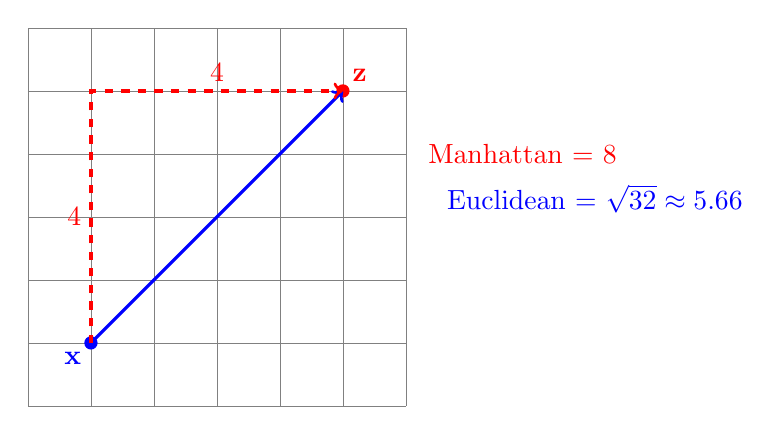
\begin{tikzpicture}[scale=0.8]
    % Grid
    \draw[step=1cm,gray,very thin] (0,0) grid (6,6);
    
    % Points
    \fill[blue] (1,1) circle (3pt) node[below left] {$\mathbf{x}$};
    \fill[red] (5,5) circle (3pt) node[above right] {$\mathbf{z}$};
    
    % Euclidean distance (straight line)
    \draw[blue, very thick, ->] (1,1) -- (5,5);
    \node[blue, above, sloped] at (9,2.9) {Euclidean = $\sqrt{32} \approx 5.66$};
    
    % Manhattan distance (grid path)
    \draw[red, very thick, dashed, ->] (1,1) -- (1,5) -- (5,5);
    \node[red, left] at (1,3) {4};
    \node[red, above] at (3,5) {4};
    \node[red, right] at (6.2,4) {Manhattan = 8};
    
\end{tikzpicture}
\end{center}

Euclidean = "as the crow flies"

Manhattan = "as a taxi drives" (only horizontal/vertical)
\end{geometrybox}

\subsection{Minkowski Distance (General Form)}

\begin{definition}[Minkowski Distance]
\begin{equation}
    d(\mathbf{x}, \mathbf{z}) = \left(\sum_{j=1}^{p}|x_j - z_j|^q\right)^{1/q}
\end{equation}

This generalizes both:
\begin{itemize}
    \item $q = 1$: Manhattan distance
    \item $q = 2$: Euclidean distance
    \item $q = \infty$: Chebyshev distance (maximum difference along any dimension)
\end{itemize}
\end{definition}

\section{Complete Numerical Example}

\begin{example}[k-NN Classification by Hand]

\textbf{Training Data:} 6 points in 2D

\begin{center}
\begin{tabular}{|c|c|c|c|}
\hline
Point & $x_1$ & $x_2$ & Class \\
\hline
$\mathbf{x}_1$ & 1 & 2 & A \\
$\mathbf{x}_2$ & 2 & 3 & A \\
$\mathbf{x}_3$ & 3 & 3 & A \\
$\mathbf{x}_4$ & 6 & 5 & B \\
$\mathbf{x}_5$ & 7 & 6 & B \\
$\mathbf{x}_6$ & 8 & 7 & B \\
\hline
\end{tabular}
\end{center}

\textbf{Query:} Classify $\mathbf{x}_{\text{new}} = [4, 4]$ using $k = 3$ and Euclidean distance.

\textbf{STEP 1: Compute distances to all training points}

\textbf{Distance to $\mathbf{x}_1 = [1, 2]$:}
\begin{align}
    d_1 &= \sqrt{(4-1)^2 + (4-2)^2} = \sqrt{9 + 4} = \sqrt{13} \approx 3.61
\end{align}

\textbf{Distance to $\mathbf{x}_2 = [2, 3]$:}
\begin{align}
    d_2 &= \sqrt{(4-2)^2 + (4-3)^2} = \sqrt{4 + 1} = \sqrt{5} \approx 2.24
\end{align}

\textbf{Distance to $\mathbf{x}_3 = [3, 3]$:}
\begin{align}
    d_3 &= \sqrt{(4-3)^2 + (4-3)^2} = \sqrt{1 + 1} = \sqrt{2} \approx 1.41
\end{align}

\textbf{Distance to $\mathbf{x}_4 = [6, 5]$:}
\begin{align}
    d_4 &= \sqrt{(4-6)^2 + (4-5)^2} = \sqrt{4 + 1} = \sqrt{5} \approx 2.24
\end{align}

\textbf{Distance to $\mathbf{x}_5 = [7, 6]$:}
\begin{align}
    d_5 &= \sqrt{(4-7)^2 + (4-6)^2} = \sqrt{9 + 4} = \sqrt{13} \approx 3.61
\end{align}

\textbf{Distance to $\mathbf{x}_6 = [8, 7]$:}
\begin{align}
    d_6 &= \sqrt{(4-8)^2 + (4-7)^2} = \sqrt{16 + 9} = \sqrt{25} = 5.00
\end{align}

\textbf{STEP 2: Create distance table and sort}

\begin{center}
\begin{tabular}{|c|c|c|c|}
\hline
Point & Distance & Class & Rank \\
\hline
$\mathbf{x}_3$ & 1.41 & A & 1 (closest) \\
$\mathbf{x}_2$ & 2.24 & A & 2 \\
$\mathbf{x}_4$ & 2.24 & B & 2 (tied) \\
$\mathbf{x}_1$ & 3.61 & A & 4 \\
$\mathbf{x}_5$ & 3.61 & B & 4 (tied) \\
$\mathbf{x}_6$ & 5.00 & B & 6 \\
\hline
\end{tabular}
\end{center}

\textbf{STEP 3: Select $k=3$ nearest neighbors}

The 3 closest points are:
\begin{enumerate}
    \item $\mathbf{x}_3$ (distance 1.41, Class A)
    \item $\mathbf{x}_2$ (distance 2.24, Class A)
    \item $\mathbf{x}_4$ (distance 2.24, Class B)
\end{enumerate}

\textbf{Note:} There's a tie at distance 2.24. We could:
\begin{itemize}
    \item Use both (making it k=4 for this query)
    \item Break tie randomly
    \item Break tie by looking at next decimal place
\end{itemize}

Let's include both $\mathbf{x}_2$ and $\mathbf{x}_4$.

\textbf{STEP 4: Majority vote}

Among the 3 nearest neighbors:
\begin{itemize}
    \item Class A: 2 votes ($\mathbf{x}_3, \mathbf{x}_2$)
    \item Class B: 1 vote ($\mathbf{x}_4$)
\end{itemize}

\textbf{Prediction: Class A wins!}

\textbf{STEP 5: Visualization}

\begin{center}
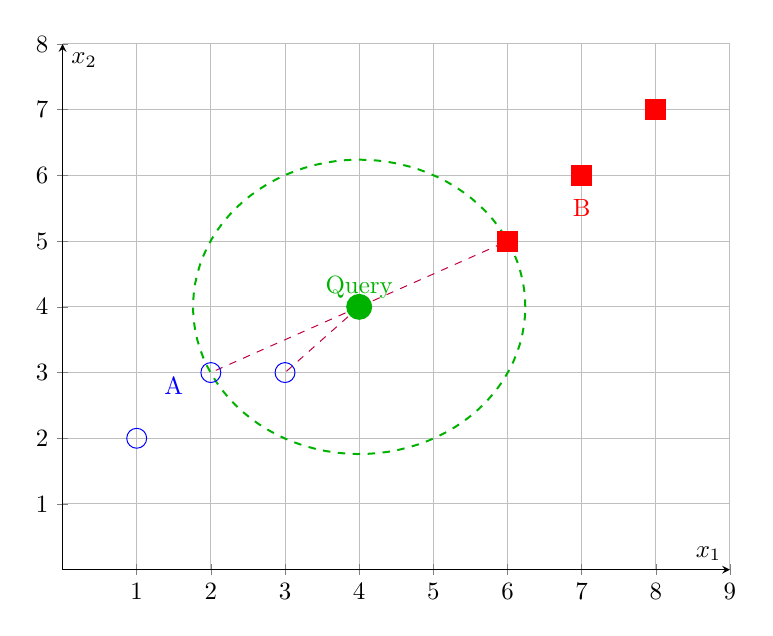
\begin{tikzpicture}[scale=0.9]
    \begin{axis}[
        axis lines = middle,
        xlabel = {$x_1$},
        ylabel = {$x_2$},
        xmin=0, xmax=9,
        ymin=0, ymax=8,
        width=11cm,
        height=9cm,
        grid=major
    ]
    
    % Class A points (circles)
    \addplot[only marks, mark=o, mark size=4pt, blue] coordinates {
        (1, 2) (2, 3) (3, 3)
    };
    \node[blue] at (1.5, 2.8) {A};
    
    % Class B points (squares)
    \addplot[only marks, mark=square*, mark size=4pt, red] coordinates {
        (6, 5) (7, 6) (8, 7)
    };
    \node[red] at (7, 5.5) {B};
    
    % Query point
    \addplot[only marks, mark=*, mark size=5pt, green!70!black] coordinates {
        (4, 4)
    };
    \node[green!70!black, above] at (4, 4) {Query};
    
    % Circle showing k=3 neighborhood
    \addplot[green!70!black, thick, dashed, domain=0:360, samples=100] 
        ({4 + 2.24*cos(x)}, {4 + 2.24*sin(x)});
    
    % Lines to 3 nearest neighbors
    \draw[purple, dashed] (4,4) -- (3,3);
    \draw[purple, dashed] (4,4) -- (2,3);
    \draw[purple, dashed] (4,4) -- (6,5);
    
    \end{axis}
\end{tikzpicture}
\end{center}

The dashed circle shows the radius containing the 3 nearest neighbors.
\end{example}

\section{k-NN for Regression}

\begin{definition}[k-NN Regression]
Instead of voting, we \textbf{average} the values of $k$ nearest neighbors:

\begin{equation}
    \hat{y} = \frac{1}{k}\sum_{i \in \mathcal{N}_k(\mathbf{x})} y_i
\end{equation}

where $\mathcal{N}_k(\mathbf{x})$ is the set of $k$ nearest neighbors of $\mathbf{x}$.
\end{definition}

\begin{example}[k-NN Regression]

\textbf{Training data:} House prices

\begin{center}
\begin{tabular}{|c|c|c|}
\hline
House & Size (1000 sq ft) & Price (\$1000s) \\
\hline
1 & 1.5 & 200 \\
2 & 2.0 & 250 \\
3 & 2.5 & 300 \\
4 & 3.0 & 350 \\
5 & 3.5 & 380 \\
\hline
\end{tabular}
\end{center}

\textbf{Query:} Predict price for size = 2.2 using $k=3$.

\textbf{Step 1: Compute distances}
\begin{align}
    d_1 &= |2.2 - 1.5| = 0.7 \\
    d_2 &= |2.2 - 2.0| = 0.2 \\
    d_3 &= |2.2 - 2.5| = 0.3 \\
    d_4 &= |2.2 - 3.0| = 0.8 \\
    d_5 &= |2.2 - 3.5| = 1.3
\end{align}

\textbf{Step 2: Find 3 nearest}

Sorted: $d_2 = 0.2, d_3 = 0.3, d_1 = 0.7, \ldots$

3 nearest: Houses 2, 3, 1

\textbf{Step 3: Average their prices}
\begin{align}
    \hat{y} &= \frac{250 + 300 + 200}{3} = \frac{750}{3} = 250
\end{align}

\textbf{Prediction: \$250,000}
\end{example}

\section{Choosing k: The Bias-Variance Trade-off}

\begin{keyidea}
The choice of $k$ is crucial and involves a bias-variance trade-off:

\textbf{Small $k$ (e.g., $k=1$):}
\begin{itemize}
    \item \textbf{Low bias:} Decision boundary is very flexible
    \item \textbf{High variance:} Sensitive to noise in training data
    \item \textbf{Risk:} Overfitting
\end{itemize}

\textbf{Large $k$ (e.g., $k=n$):}
\begin{itemize}
    \item \textbf{High bias:} Decision boundary is very smooth
    \item \textbf{Low variance:} Robust to noise
    \item \textbf{Risk:} Underfitting
\end{itemize}

\textbf{Optimal $k$:} Usually somewhere in between, found by cross-validation.
\end{keyidea}

\begin{geometrybox}
\textbf{Visualizing Different Values of $k$:}

\begin{center}
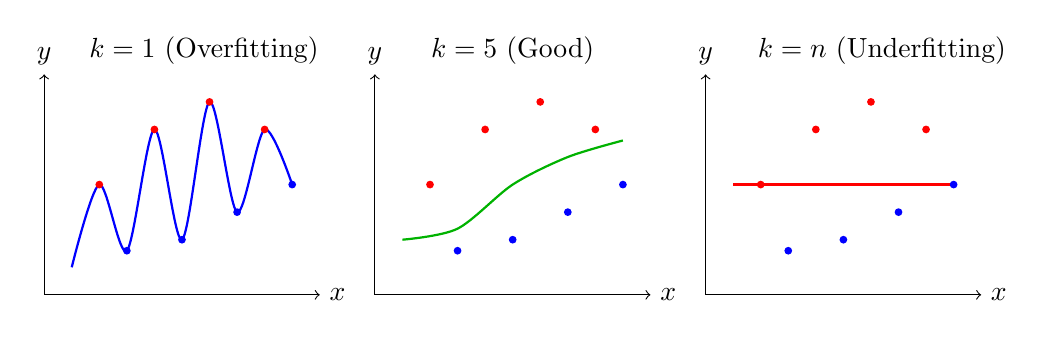
\begin{tikzpicture}[scale=0.7]
    % k=1 plot
    \begin{scope}[shift={(0,0)}]
        \draw[->] (0,0) -- (5,0) node[right] {$x$};
        \draw[->] (0,0) -- (0,4) node[above] {$y$};
        \node[above] at (2.9, 4) {$k=1$ (Overfitting)};
        
        % Very jagged decision boundary
        \draw[blue, thick] plot[smooth] coordinates {
            (0.5,0.5) (1,2) (1.5,0.8) (2,3) (2.5,1) (3,3.5) (3.5,1.5) (4,3) (4.5,2)
        };
        
        % Data points
        \foreach \x/\y in {1/2, 2/3, 3/3.5, 4/3} {
            \fill[red] (\x,\y) circle (2pt);
        }
        \foreach \x/\y in {1.5/0.8, 2.5/1, 3.5/1.5, 4.5/2} {
            \fill[blue] (\x,\y) circle (2pt);
        }
    \end{scope}
    
    % k=5 plot
    \begin{scope}[shift={(6,0)}]
        \draw[->] (0,0) -- (5,0) node[right] {$x$};
        \draw[->] (0,0) -- (0,4) node[above] {$y$};
        \node[above] at (2.5, 4) {$k=5$ (Good)};
        
        % Smooth decision boundary
        \draw[green!70!black, thick] plot[smooth] coordinates {
            (0.5,1) (1.5,1.2) (2.5,2) (3.5,2.5) (4.5,2.8)
        };
        
        % Data points
        \foreach \x/\y in {1/2, 2/3, 3/3.5, 4/3} {
            \fill[red] (\x,\y) circle (2pt);
        }
        \foreach \x/\y in {1.5/0.8, 2.5/1, 3.5/1.5, 4.5/2} {
            \fill[blue] (\x,\y) circle (2pt);
        }
    \end{scope}
    
    % k=n plot
    \begin{scope}[shift={(12,0)}]
        \draw[->] (0,0) -- (5,0) node[right] {$x$};
        \draw[->] (0,0) -- (0,4) node[above] {$y$};
        \node[above] at (3.2, 4) {$k=n$ (Underfitting)};
        
        % Almost flat line
        \draw[red, thick] (0.5,2) -- (4.5,2);
        
        % Data points
        \foreach \x/\y in {1/2, 2/3, 3/3.5, 4/3} {
            \fill[red] (\x,\y) circle (2pt);
        }
        \foreach \x/\y in {1.5/0.8, 2.5/1, 3.5/1.5, 4.5/2} {
            \fill[blue] (\x,\y) circle (2pt);
        }
    \end{scope}
\end{tikzpicture}
\end{center}

\textbf{$k=1$:} Boundary passes through every point (memorizes noise)

\textbf{$k=5$:} Smooth boundary that captures pattern

\textbf{$k=n$:} Predicts overall mean (ignores all structure)
\end{geometrybox}

\begin{example}[Effect of k on Predictions]

\textbf{Same data, different k:}

Data: $(1, 0), (2, 0), (3, 1), (4, 1), (5, 1)$

Query: $x = 2.5$

\textbf{$k=1$:} Nearest is $(3, 1)$ → Predict 1

\textbf{$k=3$:} Nearest are $(2,0), (3,1), (4,1)$ → Average = $\frac{0+1+1}{3} = 0.67$

\textbf{$k=5$:} All points → Average = $\frac{0+0+1+1+1}{5} = 0.6$

Different $k$ gives different predictions!
\end{example}

\subsection{Choosing k via Cross-Validation}

\begin{importantbox}
\textbf{Standard approach to choose $k$:}

\begin{enumerate}
    \item Try different values: $k \in \{1, 3, 5, 7, 9, \ldots, 21\}$ (typically odd numbers)
    \item For each $k$, use cross-validation to estimate error
    \item Choose $k$ with lowest CV error
\end{enumerate}

\textbf{Rule of thumb:} Try $k = \sqrt{n}$ as a starting point.

For $n = 100$: Start with $k \approx 10$
\end{importantbox}

\section{Feature Scaling is CRITICAL for k-NN}

\begin{mentalmodel}
Imagine measuring distance between houses using:
\begin{itemize}
    \item Size in sq ft: ranges from 1000 to 5000 (range = 4000)
    \item Number of bedrooms: ranges from 1 to 5 (range = 4)
\end{itemize}

Without scaling, size dominates completely!

Two houses:
\begin{itemize}
    \item House A: (2000 sq ft, 2 bedrooms)
    \item House B: (2100 sq ft, 5 bedrooms)
\end{itemize}

Distance = $\sqrt{(2100-2000)^2 + (5-2)^2} = \sqrt{100^2 + 3^2} = \sqrt{10009} \approx 100$

The bedroom difference (3) is completely ignored compared to size difference (100)!
\end{mentalmodel}

\begin{importantbox}
\textbf{ALWAYS standardize features before k-NN!}

\textbf{Standardization:}
\begin{equation}
    x_j^{\text{std}} = \frac{x_j - \mu_j}{\sigma_j}
\end{equation}

After standardization, all features have:
\begin{itemize}
    \item Mean = 0
    \item Standard deviation = 1
    \item Equal influence on distance
\end{itemize}
\end{importantbox}

\begin{example}[Effect of Scaling]

\textbf{Original data:}
\begin{itemize}
    \item Point A: Size = 2000, Bedrooms = 3
    \item Point B: Size = 2500, Bedrooms = 2
\end{itemize}

\textbf{Without scaling:}
\begin{equation}
    d = \sqrt{(2500-2000)^2 + (2-3)^2} = \sqrt{250000 + 1} \approx 500
\end{equation}

Bedroom difference contributes only 0.0004\%!

\textbf{After standardizing:}

Suppose:
\begin{itemize}
    \item Size: $\mu = 2250, \sigma = 500$
    \item Bedrooms: $\mu = 2.5, \sigma = 0.5$
\end{itemize}

Standardized:
\begin{align}
    \text{Point A:} &\left(\frac{2000-2250}{500}, \frac{3-2.5}{0.5}\right) = (-0.5, 1.0) \\
    \text{Point B:} &\left(\frac{2500-2250}{500}, \frac{2-2.5}{0.5}\right) = (0.5, -1.0)
\end{align}

\textbf{Distance:}
\begin{equation}
    d = \sqrt{(0.5-(-0.5))^2 + (-1.0-1.0)^2} = \sqrt{1 + 4} = \sqrt{5} \approx 2.24
\end{equation}

Now both features contribute equally!
\end{example}

\section{Weighted k-NN}

\begin{definition}[Weighted k-NN]
Instead of equal votes/averages, weight neighbors by inverse distance:

\textbf{For classification:}
\begin{equation}
    \text{Score for class } c = \sum_{i \in \mathcal{N}_k} w_i \cdot \mathbb{1}(y_i = c)
\end{equation}

where $w_i = \frac{1}{d(\mathbf{x}, \mathbf{x}_i)}$ or $w_i = \frac{1}{d(\mathbf{x}, \mathbf{x}_i)^2}$

\textbf{For regression:}
\begin{equation}
    \hat{y} = \frac{\sum_{i \in \mathcal{N}_k} w_i y_i}{\sum_{i \in \mathcal{N}_k} w_i}
\end{equation}

\textbf{Idea:} Closer neighbors get more influence!
\end{definition}

\begin{example}[Weighted vs Unweighted k-NN]

\textbf{3 neighbors:}
\begin{center}
\begin{tabular}{|c|c|c|}
\hline
Neighbor & Distance & Class \\
\hline
1 & 1.0 & A \\
2 & 2.0 & B \\
3 & 3.0 & B \\
\hline
\end{tabular}
\end{center}

\textbf{Unweighted:} A gets 1 vote, B gets 2 votes → Predict B

\textbf{Weighted:} (using $w_i = 1/d_i$)
\begin{align}
    \text{Score}_A &= \frac{1}{1.0} = 1.0 \\
    \text{Score}_B &= \frac{1}{2.0} + \frac{1}{3.0} = 0.5 + 0.33 = 0.83
\end{align}

Still predict B, but now it's closer! (1.0 vs 0.83 instead of 1 vs 2)

If neighbor 1 were even closer (say distance 0.5), weighted would predict A.
\end{example}

\section{The Curse of Dimensionality}

\begin{importantbox}
\textbf{Major problem with k-NN:} Performance degrades in high dimensions!

This is called the \textbf{curse of dimensionality}.
\end{importantbox}

\begin{mentalmodel}
Imagine points uniformly distributed in space:

\textbf{1D (line):} With 10 points, average spacing between neighbors is $\frac{1}{10}$ of the line

\textbf{2D (square):} With 10 points, average spacing is $\frac{1}{\sqrt{10}} \approx 0.32$ of side length

\textbf{3D (cube):} With 10 points, average spacing is $\frac{1}{\sqrt[3]{10}} \approx 0.46$

\textbf{10D (hypercube):} With 10 points, average spacing is $\frac{1}{\sqrt[10]{10}} \approx 0.79$

As dimensions increase, points become farther apart! (All neighbors are "far")
\end{mentalmodel}

\begin{theorem}[Distance Concentration]
In high dimensions, distances between points become similar:

\begin{equation}
    \frac{d_{\max} - d_{\min}}{d_{\min}} \to 0 \quad \text{as } p \to \infty
\end{equation}

The difference between nearest and farthest neighbor vanishes!

\textbf{Consequence:} The concept of "nearest neighbor" becomes meaningless.
\end{theorem}

\begin{example}[Curse of Dimensionality in Action]

\textbf{Dataset:} 1000 points

\textbf{In 2D:} The 5 nearest neighbors are much closer than the rest (clear distinction)

\textbf{In 100D:} All points are roughly equidistant! The "5 nearest" aren't much closer than the 500th nearest.

k-NN fails because there's no meaningful notion of "closeness."
\end{example}

\begin{importantbox}
\textbf{Solutions to curse of dimensionality:}
\begin{enumerate}
    \item \textbf{Feature selection:} Remove irrelevant features
    \item \textbf{Dimensionality reduction:} Use PCA (Chapter 13)
    \item \textbf{More data:} Need exponentially more data as dimensions grow
    \item \textbf{Different algorithm:} Use methods less affected (e.g., trees, neural networks)
\end{enumerate}
\end{importantbox}

\section{Computational Complexity}

\begin{definition}[Time Complexity of k-NN]

\textbf{Training:} $O(1)$ (just store data - no training!)

\textbf{Prediction for one point:}
\begin{itemize}
    \item Compute $n$ distances: $O(np)$ where $p$ = number of features
    \item Sort to find $k$ nearest: $O(n \log n)$
    \item Total: $O(np + n\log n)$
\end{itemize}

\textbf{For $m$ predictions:} $O(mnp + mn\log n)$

\textbf{Space complexity:} $O(np)$ (must store all training data)
\end{definition}

\begin{mentalmodel}
\textbf{k-NN is "lazy" during training but "eager" during prediction!}

\begin{itemize}
    \item Training: Instant (just memorize data)
    \item Prediction: Slow (must compare to all training points)
\end{itemize}

Opposite of parametric models like logistic regression:
\begin{itemize}
    \item Training: Slow (gradient descent)
    \item Prediction: Fast (just compute $\sigma(\mathbf{x}^T\boldsymbol{\beta})$)
\end{itemize}
\end{mentalmodel}

\subsection{Speeding Up k-NN: Data Structures}

\begin{definition}[KD-Tree (k-dimensional tree)]
A space-partitioning data structure that organizes points in $k$-dimensional space.

\textbf{Idea:} 
\begin{itemize}
    \item Recursively divide space using axis-aligned splits
    \item Build a binary tree
    \item Search tree to find neighbors faster than brute force
\end{itemize}

\textbf{Complexity:}
\begin{itemize}
    \item Build tree: $O(np \log n)$
    \item Query: $O(\log n)$ in low dimensions, $O(n)$ in high dimensions (curse strikes again!)
\end{itemize}
\end{definition}

\begin{note}
\textbf{Other acceleration methods:}
\begin{itemize}
    \item Ball trees (better for high dimensions than KD-trees)
    \item Locality-sensitive hashing (LSH)
    \item Approximate nearest neighbors (sacrifice exactness for speed)
\end{itemize}
\end{note}

\section{Advantages and Disadvantages of k-NN}

\begin{keyidea}
\textbf{Advantages:}
\begin{enumerate}
    \item \textbf{Simple to understand and implement}
    \item \textbf{No training phase} (fast to "learn")
    \item \textbf{No assumptions} about data distribution
    \item \textbf{Naturally handles multi-class} classification
    \item \textbf{Non-parametric:} Can model complex decision boundaries
    \item \textbf{Works for both classification and regression}
\end{enumerate}

\textbf{Disadvantages:}
\begin{enumerate}
    \item \textbf{Slow prediction} (must compare to all training data)
    \item \textbf{Memory intensive} (must store all training data)
    \item \textbf{Curse of dimensionality} (fails in high dimensions)
    \item \textbf{Sensitive to irrelevant features}
    \item \textbf{Sensitive to feature scaling} (MUST standardize)
    \item \textbf{Sensitive to noise} (especially with small $k$)
    \item \textbf{Choice of $k$ is critical}
    \item \textbf{No interpretability} (can't extract "rules" or "weights")
\end{enumerate}
\end{keyidea}

\section{GATE-Style Problems}

\begin{example}[Problem 1: Manual k-NN Classification]

\textbf{Training data:}
\begin{center}
\begin{tabular}{|c|c|c|c|}
\hline
Point & $x_1$ & $x_2$ & Class \\
\hline
A & 1 & 1 & + \\
B & 2 & 1 & + \\
C & 1 & 2 & - \\
D & 3 & 3 & - \\
\hline
\end{tabular}
\end{center}

\textbf{Query:} Classify $(2, 2)$ using $k=3$ and Euclidean distance.

\textbf{Solution:}

\textbf{Distances:}
\begin{align}
    d_A &= \sqrt{(2-1)^2 + (2-1)^2} = \sqrt{2} \approx 1.41 \\
    d_B &= \sqrt{(2-2)^2 + (2-1)^2} = 1 \\
    d_C &= \sqrt{(2-1)^2 + (2-2)^2} = 1 \\
    d_D &= \sqrt{(2-3)^2 + (2-3)^2} = \sqrt{2} \approx 1.41
\end{align}

\textbf{Sorted:} $B(1), C(1), A(1.41), D(1.41)$

\textbf{3 nearest:} B (+), C (-), A (+)

\textbf{Vote:} 2 (+) vs 1 (-) → Predict class +
\end{example}

\begin{example}[Problem 2: k-NN Regression]

\textbf{Data:} $(1, 10), (2, 15), (3, 20), (4, 25)$

\textbf{Query:} Predict $y$ for $x = 2.5$ using $k=2$.

\textbf{Solution:}

\textbf{Distances:}
\begin{align}
    d_1 &= |2.5 - 1| = 1.5 \\
    d_2 &= |2.5 - 2| = 0.5 \\
    d_3 &= |2.5 - 3| = 0.5 \\
    d_4 &= |2.5 - 4| = 1.5
\end{align}

\textbf{2 nearest:} $(2, 15)$ and $(3, 20)$

\textbf{Average:} $\hat{y} = \frac{15 + 20}{2} = 17.5$
\end{example}

\begin{example}[Problem 3: Effect of $k$]

\textbf{Question:} What happens to the decision boundary as $k$ increases from 1 to $n$?

\textbf{Answer:}

\begin{itemize}
    \item \textbf{$k=1$:} Very complex, jagged boundary (high variance, low bias)
    \item \textbf{$k$ moderate:} Smooth boundary capturing true pattern
    \item \textbf{$k=n$:} Boundary disappears (always predict majority class) (high bias, low variance)
\end{itemize}

As $k$ increases: bias increases, variance decreases.
\end{example}

\begin{example}[Problem 4: Manhattan vs Euclidean]

\textbf{Points:} $\mathbf{x} = [0, 0], \mathbf{z} = [3, 4]$

\textbf{Compute both distances.}

\textbf{Solution:}

\textbf{Euclidean:}
\begin{equation}
    d_E = \sqrt{3^2 + 4^2} = \sqrt{25} = 5
\end{equation}

\textbf{Manhattan:}
\begin{equation}
    d_M = |3| + |4| = 7
\end{equation}

Manhattan distance is larger (always $\geq$ Euclidean).
\end{example}

\begin{example}[Problem 5: Why Standardization Is Necessary in k-NN]

\textbf{Question:} Why must features be standardized for k-NN?

\medskip

\textbf{Answer:}

The k-NN algorithm is based on distance (e.g., Euclidean distance).  
Therefore, features with larger numerical scales dominate the distance computation.

\medskip

\textbf{Example:}  
Suppose we have two features:
\begin{itemize}
    \item Feature 1 ranges in $[0, 1000]$
    \item Feature 2 ranges in $[0, 1]$
\end{itemize}

Even if Feature 2 is more informative, Feature 1 will largely determine which points are considered “nearest” because its scale is much larger.

\medskip

\textbf{Conclusion:}  
Standardization (mean $=0$, standard deviation $=1$) rescales all features to a common scale, ensuring that each feature contributes fairly to the distance calculation.

\end{example}

\section{Summary - Key Points for GATE}

\begin{importantbox}
\textbf{Must Know for GATE:}

\begin{enumerate}
    \item \textbf{Algorithm:}
    \begin{enumerate}
        \item Compute distances to all training points
        \item Find $k$ nearest neighbors
        \item Classification: majority vote
        \item Regression: average
    \end{enumerate}
    
    \item \textbf{Distance metrics:}
    \begin{itemize}
        \item Euclidean: $d = \sqrt{\sum(x_j - z_j)^2}$
        \item Manhattan: $d = \sum|x_j - z_j|$
        \item Minkowski: $d = (\sum|x_j - z_j|^q)^{1/q}$
    \end{itemize}
    
    \item \textbf{Choice of $k$:}
    \begin{itemize}
        \item Small $k$: low bias, high variance (overfitting)
        \item Large $k$: high bias, low variance (underfitting)
        \item Choose via cross-validation
        \item Rule of thumb: $k \approx \sqrt{n}$
    \end{itemize}
    
    \item \textbf{Feature scaling:} MANDATORY (standardize all features)
    
    \item \textbf{Computational complexity:}
    \begin{itemize}
        \item Training: $O(1)$ (no training)
        \item Prediction: $O(np)$ per query (compare to all $n$ points)
        \item Space: $O(np)$ (store all data)
    \end{itemize}
    
    \item \textbf{Curse of dimensionality:} Fails in high dimensions (distances become meaningless)
    
    \item \textbf{Instance-based learning:} No model parameters, uses training data directly
    
    \item \textbf{Weighted k-NN:} Weight by inverse distance $w_i = 1/d_i$
    
    \item \textbf{Advantages:} Simple, no training, non-parametric, no assumptions
    
    \item \textbf{Disadvantages:} Slow prediction, memory intensive, curse of dimensionality, needs scaling
\end{enumerate}
\end{importantbox}

\begin{gatepoint}
\textbf{Common GATE Question Types:}

\begin{enumerate}
    \item Manually compute k-NN classification/regression for small dataset
    \item Calculate Euclidean/Manhattan distances
    \item Understand effect of $k$ on bias-variance
    \item Know when feature scaling is needed (ALWAYS for k-NN)
    \item Identify advantages/disadvantages
    \item Understand curse of dimensionality
    \item Compare weighted vs unweighted k-NN
    \item Computational complexity questions
    \item Know k-NN has no training phase
    \item Understand why k-NN is "lazy" learner
\end{enumerate}
\end{gatepoint}
\chapter{Naive Bayes Classifier: Probabilistic Classification}

\section{Introduction to Naive Bayes}

\begin{mentalmodel}
Imagine you're a doctor diagnosing a disease. You observe symptoms:
\begin{itemize}
    \item Patient has fever: YES
    \item Patient has cough: YES
    \item Patient has rash: NO
\end{itemize}

You know from experience:
\begin{itemize}
    \item "Flu patients usually have fever (90\%) and cough (80\%)"
    \item "Cold patients sometimes have fever (40\%) and cough (70\%)"
\end{itemize}

You use these probabilities to guess: "Given these symptoms, which disease is more likely?"

\textbf{This is Naive Bayes!}
\end{mentalmodel}

\begin{keyidea}
Naive Bayes is a \textbf{probabilistic classifier} based on Bayes' Theorem.

\textbf{Key assumption (the "naive" part):}

Features are \textbf{conditionally independent} given the class.

This is often wrong in reality, but surprisingly, Naive Bayes works well anyway!
\end{keyidea}

\section{Bayes' Theorem: The Foundation}

\begin{definition}[Bayes' Theorem]
For events $A$ and $B$:
\begin{equation}
    P(A|B) = \frac{P(B|A) \cdot P(A)}{P(B)}
\end{equation}

In words:
\begin{equation}
    \text{Posterior} = \frac{\text{Likelihood} \times \text{Prior}}{\text{Evidence}}
\end{equation}

Where:
\begin{itemize}
    \item $P(A|B)$: \textbf{Posterior} - probability of $A$ given we observed $B$
    \item $P(B|A)$: \textbf{Likelihood} - probability of observing $B$ if $A$ is true
    \item $P(A)$: \textbf{Prior} - probability of $A$ before observing $B$
    \item $P(B)$: \textbf{Evidence} - total probability of observing $B$
\end{itemize}
\end{definition}

\begin{example}[Understanding Bayes' Theorem]

\textbf{Scenario:} Medical test for a rare disease

\begin{itemize}
    \item Disease affects 1\% of population: $P(\text{Disease}) = 0.01$
    \item Test is 95\% accurate: $P(\text{Positive}|\text{Disease}) = 0.95$
    \item False positive rate 5\%: $P(\text{Positive}|\text{No Disease}) = 0.05$
\end{itemize}

\textbf{Question:} If you test positive, what's the probability you actually have the disease?

\textbf{Solution:}

We want: $P(\text{Disease}|\text{Positive})$

\textbf{Step 1:} Identify components
\begin{align}
    P(\text{Disease}) &= 0.01 \text{ (prior)} \\
    P(\text{Positive}|\text{Disease}) &= 0.95 \text{ (likelihood)}
\end{align}

\textbf{Step 2:} Calculate $P(\text{Positive})$ using law of total probability
\begin{align}
    P(\text{Positive}) &= P(\text{Positive}|\text{Disease}) \cdot P(\text{Disease}) \\
    &\quad + P(\text{Positive}|\text{No Disease}) \cdot P(\text{No Disease}) \\
    &= 0.95 \times 0.01 + 0.05 \times 0.99 \\
    &= 0.0095 + 0.0495 = 0.059
\end{align}

\textbf{Step 3:} Apply Bayes' Theorem
\begin{align}
    P(\text{Disease}|\text{Positive}) &= \frac{P(\text{Positive}|\text{Disease}) \cdot P(\text{Disease})}{P(\text{Positive})} \\
    &= \frac{0.95 \times 0.01}{0.059} \\
    &= \frac{0.0095}{0.059} \approx 0.161 = 16.1\%
\end{align}

\textbf{Surprising result:} Even with a positive test, there's only 16\% chance you have the disease!

Why? The disease is so rare that false positives outnumber true positives.
\end{example}

\section{Naive Bayes for Classification}

\subsection{The Classification Problem}

\begin{definition}[Naive Bayes Classification]
Given:
\begin{itemize}
    \item Features: $\mathbf{x} = [x_1, x_2, \ldots, x_p]^T$
    \item Classes: $y \in \{C_1, C_2, \ldots, C_K\}$
\end{itemize}

We want to find:
\begin{equation}
    \hat{y} = \arg\max_{C_k} P(y = C_k | \mathbf{x})
\end{equation}

The class with the highest posterior probability.
\end{definition}

\subsection{Applying Bayes' Theorem}

Using Bayes' Theorem:
\begin{equation}
    P(y = C_k | \mathbf{x}) = \frac{P(\mathbf{x} | y = C_k) \cdot P(y = C_k)}{P(\mathbf{x})}
\end{equation}

\begin{keyidea}
Since $P(\mathbf{x})$ is the same for all classes, we can ignore it for classification:

\begin{equation}
    \hat{y} = \arg\max_{C_k} P(\mathbf{x} | y = C_k) \cdot P(y = C_k)
\end{equation}

We only need:
\begin{itemize}
    \item $P(y = C_k)$: \textbf{Prior} - how common is class $C_k$?
    \item $P(\mathbf{x} | y = C_k)$: \textbf{Likelihood} - how likely is this feature vector for class $C_k$?
\end{itemize}
\end{keyidea}

\section{The Naive Independence Assumption}

\begin{definition}[Conditional Independence]
The \textbf{naive} assumption states that features are independent given the class:

\begin{equation}
    P(\mathbf{x} | y = C_k) = P(x_1, x_2, \ldots, x_p | y = C_k) = \prod_{j=1}^{p} P(x_j | y = C_k)
\end{equation}

The joint probability of all features given the class equals the product of individual probabilities.
\end{definition}

\begin{mentalmodel}
\textbf{What does "conditional independence" mean?}

Given the class, knowing one feature tells you nothing about other features.

\textbf{Example (Email Spam):}
\begin{itemize}
    \item Features: word "free", word "money", number of exclamation marks
    \item Class: Spam or Ham
\end{itemize}

Naive assumption: "Given it's spam, the presence of 'free' is independent of the presence of 'money'."

This is obviously false! Spam emails with "free" are more likely to also have "money".

But we make this assumption anyway because:
\begin{enumerate}
    \item Makes computation tractable
    \item Surprisingly works well in practice
\end{enumerate}
\end{mentalmodel}

\subsection{The Final Classification Rule}

\begin{theorem}[Naive Bayes Classifier]
\begin{equation}
    \boxed{\hat{y} = \arg\max_{C_k} \left[P(y = C_k) \prod_{j=1}^{p} P(x_j | y = C_k)\right]}
\end{equation}

Or equivalently, using log (to avoid numerical underflow):
\begin{equation}
    \hat{y} = \arg\max_{C_k} \left[\log P(y = C_k) + \sum_{j=1}^{p} \log P(x_j | y = C_k)\right]
\end{equation}
\end{theorem}

\begin{importantbox}
\textbf{What we need to learn from training data:}

\begin{enumerate}
    \item \textbf{Class priors:} $P(y = C_k)$ for each class
    \item \textbf{Conditional probabilities:} $P(x_j | y = C_k)$ for each feature $j$ and class $k$
\end{enumerate}

These are estimated from the training data!
\end{importantbox}

\section{Learning from Data}

\subsection{Estimating Class Priors}

\begin{definition}[Maximum Likelihood Estimate of Prior]
Given training data with $n$ examples:

\begin{equation}
    P(y = C_k) = \frac{n_k}{n}
\end{equation}

where $n_k$ is the number of training examples in class $C_k$.

\textbf{Simply:} The fraction of training data in each class.
\end{definition}

\begin{example}[Computing Priors]

\textbf{Training data:} 100 emails
\begin{itemize}
    \item 60 are Ham (not spam)
    \item 40 are Spam
\end{itemize}

\begin{align}
    P(y = \text{Ham}) &= \frac{60}{100} = 0.6 \\
    P(y = \text{Spam}) &= \frac{40}{100} = 0.4
\end{align}
\end{example}

\subsection{Estimating Conditional Probabilities}

How we estimate $P(x_j | y = C_k)$ depends on the type of feature.

\section{Types of Naive Bayes}

\subsection{Gaussian Naive Bayes (Continuous Features)}

\begin{definition}[Gaussian Naive Bayes]
For continuous features, assume each $P(x_j | y = C_k)$ follows a Gaussian (normal) distribution:

\begin{equation}
    P(x_j | y = C_k) = \frac{1}{\sqrt{2\pi\sigma_{jk}^2}} \exp\left(-\frac{(x_j - \mu_{jk})^2}{2\sigma_{jk}^2}\right)
\end{equation}

where:
\begin{itemize}
    \item $\mu_{jk}$: mean of feature $j$ in class $k$
    \item $\sigma_{jk}^2$: variance of feature $j$ in class $k$
\end{itemize}

We estimate from training data:
\begin{align}
    \mu_{jk} &= \frac{1}{n_k}\sum_{i: y_i = C_k} x_{ij} \\
    \sigma_{jk}^2 &= \frac{1}{n_k}\sum_{i: y_i = C_k} (x_{ij} - \mu_{jk})^2
\end{align}
\end{definition}

\begin{example}[Gaussian Naive Bayes - Height Classification]

\textbf{Problem:} Classify gender based on height and weight

\textbf{Training data:}

\textbf{Males:} Heights (cm) = [175, 180, 178, 182, 177]

\textbf{Females:} Heights (cm) = [160, 165, 162, 158, 163]

\textbf{Step 1: Estimate priors}
\begin{align}
    P(\text{Male}) &= \frac{5}{10} = 0.5 \\
    P(\text{Female}) &= \frac{5}{10} = 0.5
\end{align}

\textbf{Step 2: Estimate parameters for height}

For Males:
\begin{align}
    \mu_{\text{Male}} &= \frac{175 + 180 + 178 + 182 + 177}{5} = \frac{892}{5} = 178.4 \\
    \sigma_{\text{Male}}^2 &= \frac{(175-178.4)^2 + (180-178.4)^2 + \cdots}{5} \\
    &= \frac{11.56 + 2.56 + 0.16 + 12.96 + 1.96}{5} = \frac{29.2}{5} = 5.84 \\
    \sigma_{\text{Male}} &= \sqrt{5.84} \approx 2.42
\end{align}

For Females:
\begin{align}
    \mu_{\text{Female}} &= \frac{160 + 165 + 162 + 158 + 163}{5} = \frac{808}{5} = 161.6 \\
    \sigma_{\text{Female}}^2 &= \frac{(160-161.6)^2 + \cdots}{5} \\
    &= \frac{2.56 + 11.56 + 0.16 + 12.96 + 1.96}{5} = \frac{29.2}{5} = 5.84 \\
    \sigma_{\text{Female}} &\approx 2.42
\end{align}

\textbf{Step 3: Classify new person with height = 170 cm}

\textbf{For Male:}
\begin{align}
    P(170|\text{Male}) &= \frac{1}{\sqrt{2\pi \cdot 5.84}} \exp\left(-\frac{(170-178.4)^2}{2 \cdot 5.84}\right) \\
    &= \frac{1}{6.05} \exp\left(-\frac{70.56}{11.68}\right) \\
    &= 0.165 \times \exp(-6.04) \\
    &\approx 0.165 \times 0.0024 = 0.000396
\end{align}

\textbf{For Female:}
\begin{align}
    P(170|\text{Female}) &= \frac{1}{\sqrt{2\pi \cdot 5.84}} \exp\left(-\frac{(170-161.6)^2}{2 \cdot 5.84}\right) \\
    &= 0.165 \times \exp\left(-\frac{70.56}{11.68}\right) \\
    &\approx 0.165 \times 0.0024 = 0.000396
\end{align}

Wait, they're the same! Because we got the same variance. Let me recalculate more carefully.

Actually, let's use the formula directly:

\begin{align}
    P(\text{Male}|170) &\propto P(\text{Male}) \times P(170|\text{Male}) \\
    &\propto 0.5 \times \exp\left(-\frac{(170-178.4)^2}{2 \cdot 5.84}\right) \\
    &\propto 0.5 \times \exp(-6.04) \approx 0.5 \times 0.0024 = 0.0012
\end{align}

\begin{align}
    P(\text{Female}|170) &\propto 0.5 \times \exp\left(-\frac{(170-161.6)^2}{2 \cdot 5.84}\right) \\
    &\propto 0.5 \times \exp(-6.04) \approx 0.0012
\end{align}

Since $170$ is exactly between the two means, this makes sense. Let's try height = 165:

\begin{align}
    P(\text{Male}|165) &\propto 0.5 \times \exp\left(-\frac{(165-178.4)^2}{11.68}\right) \\
    &\propto 0.5 \times \exp(-15.36) \approx 0
\end{align}

\begin{align}
    P(\text{Female}|165) &\propto 0.5 \times \exp\left(-\frac{(165-161.6)^2}{11.68}\right) \\
    &\propto 0.5 \times \exp(-0.99) \approx 0.5 \times 0.37 = 0.185
\end{align}

\textbf{Prediction: Female} (much higher probability)
\end{example}

\subsection{Multinomial Naive Bayes (Count Features)}

\begin{definition}[Multinomial Naive Bayes]
For count data (e.g., word frequencies in text):

\begin{equation}
    P(x_j | y = C_k) = \frac{N_{jk} + \alpha}{N_k + \alpha p}
\end{equation}

where:
\begin{itemize}
    \item $N_{jk}$: count of feature $j$ in class $k$ examples
    \item $N_k$: total count of all features in class $k$ examples
    \item $\alpha$: smoothing parameter (typically 1, called "Laplace smoothing")
    \item $p$: number of features
\end{itemize}

\textbf{Used for:} Text classification, document categorization
\end{definition}

\subsection{Bernoulli Naive Bayes (Binary Features)}

\begin{definition}[Bernoulli Naive Bayes]
For binary features (presence/absence):

\begin{equation}
    P(x_j | y = C_k) = \begin{cases}
        \theta_{jk} & \text{if } x_j = 1 \\
        1 - \theta_{jk} & \text{if } x_j = 0
    \end{cases}
\end{equation}

where $\theta_{jk} = P(x_j = 1 | y = C_k)$ is estimated as:

\begin{equation}
    \theta_{jk} = \frac{\text{count}(x_j = 1 \text{ and } y = C_k) + \alpha}{\text{count}(y = C_k) + 2\alpha}
\end{equation}

\textbf{Used for:} Binary feature classification (word present/absent in document)
\end{definition}

\section{Complete Numerical Example: Email Spam Classification}

\begin{example}[Multinomial Naive Bayes by Hand]

\textbf{Training data:} 6 emails with word counts

\begin{center}
\begin{tabular}{|c|c|c|c|c|}
\hline
Email & "free" & "money" & "meet" & Class \\
\hline
1 & 2 & 1 & 0 & Spam \\
2 & 3 & 2 & 0 & Spam \\
3 & 1 & 1 & 0 & Spam \\
4 & 0 & 0 & 2 & Ham \\
5 & 0 & 0 & 1 & Ham \\
6 & 0 & 0 & 3 & Ham \\
\hline
\end{tabular}
\end{center}

\textbf{Test email:} "free" = 1, "money" = 0, "meet" = 1

\textbf{STEP 1: Compute class priors}

\begin{align}
    P(\text{Spam}) &= \frac{3}{6} = 0.5 \\
    P(\text{Ham}) &= \frac{3}{6} = 0.5
\end{align}

\textbf{STEP 2: Count feature occurrences per class}

\textbf{Spam class (3 emails):}
\begin{align}
    \text{count("free"|Spam)} &= 2 + 3 + 1 = 6 \\
    \text{count("money"|Spam)} &= 1 + 2 + 1 = 4 \\
    \text{count("meet"|Spam)} &= 0 + 0 + 0 = 0 \\
    \text{Total words in Spam} &= 6 + 4 + 0 = 10
\end{align}

\textbf{Ham class (3 emails):}
\begin{align}
    \text{count("free"|Ham)} &= 0 + 0 + 0 = 0 \\
    \text{count("money"|Ham)} &= 0 + 0 + 0 = 0 \\
    \text{count("meet"|Ham)} &= 2 + 1 + 3 = 6 \\
    \text{Total words in Ham} &= 0 + 0 + 6 = 6
\end{align}

\textbf{STEP 3: Estimate conditional probabilities with Laplace smoothing ($\alpha = 1$)}

Number of features $p = 3$

\textbf{For Spam:}
\begin{align}
    P(\text{"free"}|\text{Spam}) &= \frac{6 + 1}{10 + 1 \times 3} = \frac{7}{13} \approx 0.538 \\
    P(\text{"money"}|\text{Spam}) &= \frac{4 + 1}{10 + 3} = \frac{5}{13} \approx 0.385 \\
    P(\text{"meet"}|\text{Spam}) &= \frac{0 + 1}{10 + 3} = \frac{1}{13} \approx 0.077
\end{align}

\textbf{For Ham:}
\begin{align}
    P(\text{"free"}|\text{Ham}) &= \frac{0 + 1}{6 + 3} = \frac{1}{9} \approx 0.111 \\
    P(\text{"money"}|\text{Ham}) &= \frac{0 + 1}{6 + 3} = \frac{1}{9} \approx 0.111 \\
    P(\text{"meet"}|\text{Ham}) &= \frac{6 + 1}{6 + 3} = \frac{7}{9} \approx 0.778
\end{align}

\textbf{STEP 4: Classify test email: "free"=1, "money"=0, "meet"=1}

For multinomial NB, we compute the probability of seeing this exact count vector.

Actually, for simplicity, let's treat this as Bernoulli (presence/absence):

Features present: "free" and "meet"

Feature absent: "money"

\textbf{For Spam:}
\begin{align}
    P(\text{Spam}|\mathbf{x}) &\propto P(\text{Spam}) \times P(\text{free}=1|\text{Spam}) \\
    &\quad \times P(\text{money}=0|\text{Spam}) \times P(\text{meet}=1|\text{Spam}) \\
    &\propto 0.5 \times 0.538 \times (1-0.385) \times 0.077 \\
    &\propto 0.5 \times 0.538 \times 0.615 \times 0.077 \\
    &\approx 0.0127
\end{align}

\textbf{For Ham:}
\begin{align}
    P(\text{Ham}|\mathbf{x}) &\propto 0.5 \times P(\text{free}=1|\text{Ham}) \\
    &\quad \times P(\text{money}=0|\text{Ham}) \times P(\text{meet}=1|\text{Ham}) \\
    &\propto 0.5 \times 0.111 \times (1-0.111) \times 0.778 \\
    &\propto 0.5 \times 0.111 \times 0.889 \times 0.778 \\
    &\approx 0.0384
\end{align}

\textbf{Comparison:}
\begin{align}
    P(\text{Spam}|\mathbf{x}) &\approx 0.0127 \\
    P(\text{Ham}|\mathbf{x}) &\approx 0.0384
\end{align}

Since $0.0384 > 0.0127$:

\textbf{Prediction: Ham (Not Spam)}

Makes sense! The word "meet" is strongly associated with Ham emails.
\end{example}

\section{Laplace Smoothing}

\begin{importantbox}
\textbf{The Zero-Frequency Problem:}

What if a word never appears in training data for a class?

Example: Word "lottery" never appears in Ham emails.

Then $P(\text{"lottery"}|\text{Ham}) = 0$

\textbf{Problem:} If test email has "lottery", the entire product becomes 0!

\begin{equation}
    P(\text{Ham}|\mathbf{x}) \propto P(\text{Ham}) \times 0 \times \cdots = 0
\end{equation}

Ham would have 0 probability, even if all other words suggest Ham.
\end{importantbox}

\begin{definition}[Laplace Smoothing (Add-One Smoothing)]
Instead of:
\begin{equation}
    P(x_j | y = C_k) = \frac{\text{count}(x_j, C_k)}{\text{count}(C_k)}
\end{equation}

Use:
\begin{equation}
    P(x_j | y = C_k) = \frac{\text{count}(x_j, C_k) + \alpha}{\text{count}(C_k) + \alpha V}
\end{equation}

where:
\begin{itemize}
    \item $\alpha$: smoothing parameter (typically 1)
    \item $V$: vocabulary size (number of possible values for feature $x_j$)
\end{itemize}

\textbf{Effect:} No probability is ever exactly 0!
\end{definition}

\begin{example}[Laplace Smoothing Effect]

\textbf{Without smoothing:}

Word "lottery" appears 0 times in 100 Ham emails:
\begin{equation}
    P(\text{"lottery"}|\text{Ham}) = \frac{0}{100} = 0
\end{equation}

\textbf{With Laplace smoothing ($\alpha=1$, vocabulary size $V=1000$):}
\begin{equation}
    P(\text{"lottery"}|\text{Ham}) = \frac{0 + 1}{100 + 1000} = \frac{1}{1100} \approx 0.00091
\end{equation}

Very small, but not zero! The model can still function.
\end{example}

\section{Advantages and Disadvantages}

\begin{keyidea}
\textbf{Advantages:}

\begin{enumerate}
    \item \textbf{Simple and fast:} Easy to implement and train
    \item \textbf{Scalable:} Works well with high-dimensional data (e.g., text with 10,000+ words)
    \item \textbf{Works with small training sets:} Doesn't need massive data
    \item \textbf{Handles missing data:} Can ignore features not present
    \item \textbf{Multi-class classification:} Naturally extends to $K > 2$ classes
    \item \textbf{Probabilistic:} Outputs probabilities, not just class labels
    \item \textbf{Online learning:} Can update model as new data arrives
    \item \textbf{Good baseline:} Often surprisingly competitive with more complex methods
\end{enumerate}

\textbf{Disadvantages:}

\begin{enumerate}
    \item \textbf{"Naive" assumption often violated:} Features are rarely independent
    \item \textbf{Zero-frequency problem:} Needs smoothing
    \item \textbf{Poor probability estimates:} Probabilities can be poorly calibrated (but classifications often still good)
    \item \textbf{Sensitive to irrelevant features:} All features contribute to decision
    \item \textbf{Assumes feature independence:} Can't capture feature interactions
    \item \textbf{Distribution assumptions:} Gaussian NB assumes normality, etc.
\end{enumerate}
\end{keyidea}

\section{Why Does Naive Bayes Work Despite Being "Naive"?}

\begin{mentalmodel}
\textbf{The Paradox:}

The independence assumption is almost always wrong in real data, yet Naive Bayes often works well!

\textbf{Why?}

\begin{enumerate}
    \item \textbf{We only need the ranking of probabilities, not exact values}
    
    Even if $P(C_k|\mathbf{x})$ is wrong, as long as $P(C_1|\mathbf{x}) > P(C_2|\mathbf{x})$ is correct, we classify correctly!
    
    \item \textbf{Errors can cancel out}
    
    Overestimating probability for one feature might be offset by underestimating another.
    
    \item \textbf{Robust to many dependencies}
    
    The independence assumption needs to be violated very severely before classifications become wrong.
    
    \item \textbf{Low variance}
    
    Simple model with few parameters → less prone to overfitting.
\end{enumerate}
\end{mentalmodel}

\begin{theorem}[Naive Bayes Optimality]
Naive Bayes is the optimal classifier if:
\begin{enumerate}
    \item Features truly are conditionally independent given the class
    \item We have infinite training data
    \item Feature distributions are correctly specified (e.g., truly Gaussian)
\end{enumerate}

In practice, none of these hold, but it still works reasonably well!
\end{theorem}

\section{Computational Complexity}

\begin{definition}[Complexity Analysis]

\textbf{Training:} $O(np)$
\begin{itemize}
    \item Must scan through $n$ examples
    \item For each, update counts for $p$ features
    \item Very fast!
\end{itemize}

\textbf{Prediction:} $O(Kp)$
\begin{itemize}
    \item For each of $K$ classes
    \item Compute product over $p$ features
    \item Very fast!
\end{itemize}

\textbf{Space:} $O(Kp)$
\begin{itemize}
    \item Store $P(x_j|y=C_k)$ for each feature and class
    \item Very memory efficient!
\end{itemize}

\textbf{Comparison with k-NN:}
\begin{itemize}
    \item k-NN: $O(1)$ training, $O(np)$ prediction
    \item Naive Bayes: $O(np)$ training, $O(Kp)$ prediction
\end{itemize}

Naive Bayes is much faster for prediction when $K << n$!
\end{definition}

\section{GATE-Style Problems}

\begin{example}[Problem 1: Binary Naive Bayes by Hand]

\textbf{Training data:}
\begin{center}
\begin{tabular}{|c|c|c|c|}
\hline
\# & Fever & Cough & Disease \\
\hline
1 & Yes & Yes & Flu \\
2 & Yes & No & Flu \\
3 & No & Yes & Cold \\
4 & No & No & Cold \\
\hline
\end{tabular}
\end{center}

\textbf{Query:} Patient has Fever=Yes, Cough=Yes. Diagnose disease.

\textbf{Solution:}

\textbf{Step 1: Priors}
\begin{align}
    P(\text{Flu}) &= \frac{2}{4} = 0.5 \\
    P(\text{Cold}) &= \frac{2}{4} = 0.5
\end{align}

\textbf{Step 2: Conditional probabilities}

For Flu (2 examples):
\begin{align}
    P(\text{Fever=Yes}|\text{Flu}) &= \frac{2}{2} = 1.0 \\
    P(\text{Cough=Yes}|\text{Flu}) &= \frac{1}{2} = 0.5
\end{align}

For Cold (2 examples):
\begin{align}
    P(\text{Fever=Yes}|\text{Cold}) &= \frac{0}{2} = 0 \\
    P(\text{Cough=Yes}|\text{Cold}) &= \frac{1}{2} = 0.5
\end{align}

\textbf{Step 3: Classify}

\begin{align}
    P(\text{Flu}|\text{FY, CY}) &\propto 0.5 \times 1.0 \times 0.5 = 0.25 \\
    P(\text{Cold}|\text{FY, CY}) &\propto 0.5 \times 0 \times 0.5 = 0
\end{align}

\textbf{Prediction: Flu}

Note: Cold got 0 because no Cold patient had fever! This is where we'd use Laplace smoothing in practice.
\end{example}

\begin{example}[Problem 2: With Laplace Smoothing]

Same data, apply Laplace smoothing with $\alpha = 1$.

For binary features, denominator becomes: $\text{count}(C_k) + 2\alpha$

\textbf{For Flu:}
\begin{align}
    P(\text{Fever=Yes}|\text{Flu}) &= \frac{2 + 1}{2 + 2} = \frac{3}{4} = 0.75 \\
    P(\text{Cough=Yes}|\text{Flu}) &= \frac{1 + 1}{2 + 2} = \frac{2}{4} = 0.5
\end{align}

\textbf{For Cold:}
\begin{align}
    P(\text{Fever=Yes}|\text{Cold}) &= \frac{0 + 1}{2 + 2} = \frac{1}{4} = 0.25 \\
    P(\text{Cough=Yes}|\text{Cold}) &= \frac{1 + 1}{2 + 2} = \frac{2}{4} = 0.5
\end{align}

\textbf{Classify:}
\begin{align}
    P(\text{Flu}|\text{FY, CY}) &\propto 0.5 \times 0.75 \times 0.5 = 0.1875 \\
    P(\text{Cold}|\text{FY, CY}) &\propto 0.5 \times 0.25 \times 0.5 = 0.0625
\end{align}

\textbf{Prediction: Still Flu, but Cold now has non-zero probability!}
\end{example}

\begin{example}[Problem 3: Gaussian Naive Bayes]

\textbf{Given:}
\begin{itemize}
    \item Class A: $\mu_1 = 5, \sigma_1 = 1$
    \item Class B: $\mu_2 = 8, \sigma_2 = 1$
    \item $P(A) = P(B) = 0.5$
\end{itemize}

\textbf{Question:} Classify $x = 6.5$

\textbf{Solution:}

\begin{align}
    P(6.5|A) &\propto \exp\left(-\frac{(6.5-5)^2}{2 \cdot 1^2}\right) = \exp(-1.125) \approx 0.325 \\
    P(6.5|B) &\propto \exp\left(-\frac{(6.5-8)^2}{2 \cdot 1^2}\right) = \exp(-1.125) \approx 0.325
\end{align}

They're equal! Makes sense - 6.5 is exactly halfway between 5 and 8.

\textbf{Prediction: Tie (could go either way)}

For $x = 6$:
\begin{align}
    P(6|A) &\propto \exp(-0.5) \approx 0.606 \\
    P(6|B) &\propto \exp(-2) \approx 0.135
\end{align}

\textbf{Prediction: Class A} (closer to mean of 5)
\end{example}

\begin{example}[Problem 4: Understanding Independence Assumption]

\textbf{Question:} What does the naive independence assumption mean?

\textbf{Answer:}

The assumption is: $P(x_1, x_2 | y) = P(x_1|y) \cdot P(x_2|y)$

\textbf{In words:} "Given the class, knowing feature $x_1$ tells you nothing about feature $x_2$."

\textbf{Example where it's violated:}
\begin{itemize}
    \item Features: Temperature, Ice cream sales
    \item Class: Season (Summer/Winter)
\end{itemize}

Given it's summer, high temperature and high ice cream sales are correlated (not independent).

But Naive Bayes assumes they're independent given the season.
\end{example}

\section{Summary - Key Points for GATE}

\begin{importantbox}
\textbf{Must Know for GATE:}

\begin{enumerate}
    \item \textbf{Bayes' Theorem:}
    \begin{equation}
        P(A|B) = \frac{P(B|A) \cdot P(A)}{P(B)}
    \end{equation}
    
    \item \textbf{Naive Bayes Classification:}
    \begin{equation}
        \hat{y} = \arg\max_{C_k} \left[P(y=C_k) \prod_{j=1}^{p} P(x_j|y=C_k)\right]
    \end{equation}
    
    \item \textbf{Independence assumption:} Features are conditionally independent given class
    \begin{equation}
        P(\mathbf{x}|y=C_k) = \prod_{j=1}^{p} P(x_j|y=C_k)
    \end{equation}
    
    \item \textbf{Prior estimation:} $P(y=C_k) = \frac{n_k}{n}$
    
    \item \textbf{Types of Naive Bayes:}
    \begin{itemize}
        \item Gaussian: continuous features (assumes normal distribution)
        \item Multinomial: count features (word frequencies)
        \item Bernoulli: binary features (presence/absence)
    \end{itemize}
    
    \item \textbf{Laplace smoothing:} Add $\alpha$ to counts to avoid zero probabilities
    \begin{equation}
        P(x_j|y=C_k) = \frac{\text{count}(x_j, C_k) + \alpha}{\text{count}(C_k) + \alpha V}
    \end{equation}
    
    \item \textbf{Complexity:} Training $O(np)$, Prediction $O(Kp)$, Space $O(Kp)$
    
    \item \textbf{Why "naive"?} Assumes independence (usually violated)
    
    \item \textbf{Why it works anyway?} Only need ranking correct, not exact probabilities
    
    \item \textbf{Advantages:} Fast, scalable, works with small data, multi-class
    
    \item \textbf{Disadvantages:} Independence assumption, zero-frequency problem, poor probability calibration
\end{enumerate}
\end{importantbox}

\begin{gatepoint}
\textbf{Common GATE Question Types:}

\begin{enumerate}
    \item Apply Bayes' theorem to compute posterior probabilities
    \item Manually compute Naive Bayes classification for small dataset
    \item Calculate class priors from training data
    \item Estimate conditional probabilities for different feature types
    \item Apply Laplace smoothing
    \item Explain the independence assumption
    \item Why does NB work despite violated assumptions?
    \item Compare computational complexity with other methods
    \item Identify which type of NB for given problem (Gaussian/Multinomial/Bernoulli)
    \item Understand when zero-probability problem occurs
\end{enumerate}
\end{gatepoint}
\chapter{Linear Discriminant Analysis (LDA): Fisher's Approach}

\section{Introduction to LDA}

\begin{mentalmodel}
Imagine you have two groups of students: one that passed an exam and one that failed. You measure two things for each student: study hours and sleep hours.

Now you want to draw a single line (1D) such that when you project all students onto this line, the two groups are \textbf{maximally separated}.

\textbf{This is the essence of Linear Discriminant Analysis!}

LDA finds the "best direction" to separate classes.
\end{mentalmodel}

\begin{keyidea}
Linear Discriminant Analysis (LDA) is both:
\begin{enumerate}
    \item A \textbf{classification algorithm} (like logistic regression, Naive Bayes)
    \item A \textbf{dimensionality reduction technique} (like PCA)
\end{enumerate}

\textbf{Core idea:} Find a linear combination of features that best separates classes.

\textbf{Key difference from other methods:}
\begin{itemize}
    \item Logistic regression: Directly models $P(y|x)$
    \item Naive Bayes: Models $P(x|y)$ and uses Bayes' theorem
    \item LDA: Models $P(x|y)$ assuming Gaussian distributions, finds optimal projection
\end{itemize}
\end{keyidea}

\section{The Two-Class Problem}

\subsection{Problem Setup}

\begin{definition}[Two-Class LDA Setup]
Given:
\begin{itemize}
    \item Two classes: $C_1$ and $C_2$
    \item Data points: $\mathbf{x} \in \mathbb{R}^p$ ($p$-dimensional features)
    \item Class 1: $n_1$ samples with mean $\boldsymbol{\mu}_1$
    \item Class 2: $n_2$ samples with mean $\boldsymbol{\mu}_2$
\end{itemize}

\textbf{Goal:} Find a direction (vector) $\mathbf{w} \in \mathbb{R}^p$ such that when we project data onto $\mathbf{w}$, the two classes are well-separated.

\textbf{Projection:} $y = \mathbf{w}^T\mathbf{x}$ (scalar value)
\end{definition}

\begin{geometrybox}
\textbf{Visualizing LDA Projection (2D to 1D):}

\begin{center}
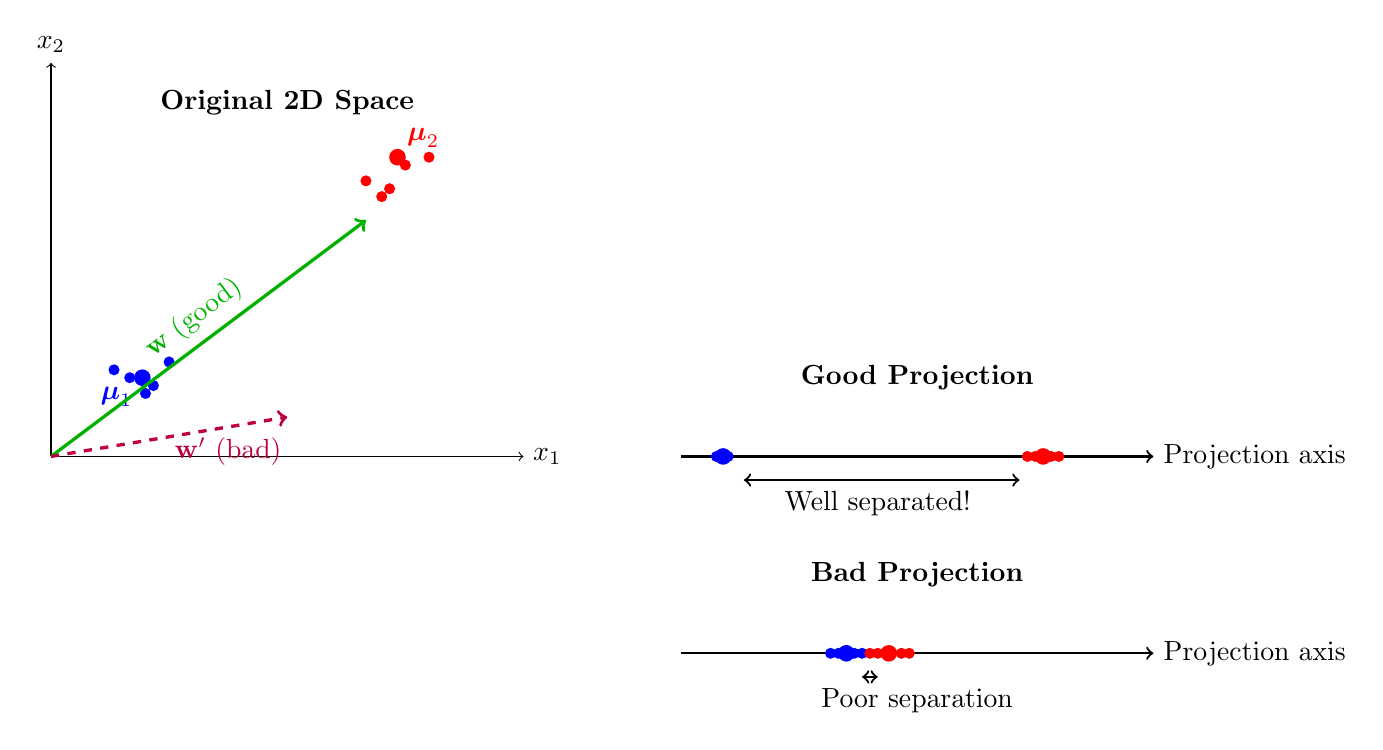
\begin{tikzpicture}[scale=1.0]
    % Original 2D space
    \begin{scope}
        \draw[->] (0,0) -- (6,0) node[right] {$x_1$};
        \draw[->] (0,0) -- (0,5) node[above] {$x_2$};
        
        % Class 1 points (blue circles)
        \foreach \x/\y in {1/1, 1.5/1.2, 1.2/0.8, 0.8/1.1, 1.3/0.9} {
            \fill[blue] (\x,\y) circle (2pt);
        }
        
        % Class 2 points (red circles)
        \foreach \x/\y in {4/3.5, 4.5/3.7, 4.2/3.3, 4.8/3.8, 4.3/3.4} {
            \fill[red] (\x,\y) circle (2pt);
        }
        
        % Class means
        \fill[blue] (1.16,1.0) circle (3pt) node[below left] {$\boldsymbol{\mu}_1$};
        \fill[red] (4.4,3.80) circle (3pt) node[above right] {$\boldsymbol{\mu}_2$};
        
        % Good projection direction
        \draw[->, very thick, green!70!black] (0,0) -- (4,3) node[midway, above, sloped] {$\mathbf{w}$ (good)};
        
        % Bad projection direction
        \draw[->, very thick, purple, dashed] (0,0) -- (3,0.5) node[near end, below] {$\mathbf{w}'$ (bad)};
        
        \node at (3, 4.5) {\textbf{Original 2D Space}};
    \end{scope}
    
    % Projected 1D space (good projection)
    \begin{scope}[shift={(8,0)}]
        \draw[->, thick] (0,0) -- (6,0) node[right] {Projection axis};
        
        % Projected class 1 (clustered on left)
        \foreach \pos in {0.5, 0.6, 0.55, 0.45, 0.58} {
            \fill[blue] (\pos, 0) circle (2pt);
        }
        
        % Projected class 2 (clustered on right)
        \foreach \pos in {4.5, 4.7, 4.4, 4.8, 4.6} {
            \fill[red] (\pos, 0) circle (2pt);
        }
        
        % Means
        \fill[blue] (0.536, 0) circle (3pt);
        \fill[red] (4.6, 0) circle (3pt);
        
        % Separation
        \draw[<->, thick] (0.8, -0.3) -- (4.3, -0.3);
        \node at (2.5, -0.6) {Well separated!};
        
        \node at (3, 1) {\textbf{Good Projection}};
    \end{scope}
    
    % Projected 1D space (bad projection)
    \begin{scope}[shift={(8,-2.5)}]
        \draw[->, thick] (0,0) -- (6,0) node[right] {Projection axis};
        
        % Projected classes overlap
        \foreach \pos in {2.0, 2.3, 2.1, 1.9, 2.2} {
            \fill[blue] (\pos, 0) circle (2pt);
        }
        \foreach \pos in {2.5, 2.8, 2.4, 2.9, 2.6} {
            \fill[red] (\pos, 0) circle (2pt);
        }
        
        % Means
        \fill[blue] (2.1, 0) circle (3pt);
        \fill[red] (2.64, 0) circle (3pt);
        
        % Little separation
        \draw[<->, thick] (2.3, -0.3) -- (2.5, -0.3);
        \node at (3, -0.6) {Poor separation};
        
        \node at (3, 1) {\textbf{Bad Projection}};
    \end{scope}
\end{tikzpicture}
\end{center}

The good projection $\mathbf{w}$ creates clear separation; the bad projection $\mathbf{w}'$ creates overlap.
\end{geometrybox}

\section{Fisher's Linear Discriminant}

\subsection{What Makes a Good Projection?}

\begin{mentalmodel}
A good projection should:
\begin{enumerate}
    \item Maximize the distance between class means (push classes apart)
    \item Minimize the spread within each class (keep classes tight)
\end{enumerate}

Think of it like: "Push the class centers far apart while keeping each class clustered."
\end{mentalmodel}

\subsection{Mathematical Formulation}

After projecting onto $\mathbf{w}$, each point $\mathbf{x}$ becomes scalar $y = \mathbf{w}^T\mathbf{x}$.

\begin{definition}[Projected Means]
The mean of projected class 1:
\begin{equation}
    m_1 = \mathbf{w}^T\boldsymbol{\mu}_1
\end{equation}

The mean of projected class 2:
\begin{equation}
    m_2 = \mathbf{w}^T\boldsymbol{\mu}_2
\end{equation}

The distance between projected means:
\begin{equation}
    (m_1 - m_2)^2 = (\mathbf{w}^T\boldsymbol{\mu}_1 - \mathbf{w}^T\boldsymbol{\mu}_2)^2 = (\mathbf{w}^T(\boldsymbol{\mu}_1 - \boldsymbol{\mu}_2))^2
\end{equation}
\end{definition}

\begin{definition}[Within-Class Variance]
The variance of projected class $k$:
\begin{equation}
    s_k^2 = \sum_{i \in C_k} (y_i - m_k)^2 = \sum_{i \in C_k} (\mathbf{w}^T\mathbf{x}_i - \mathbf{w}^T\boldsymbol{\mu}_k)^2
\end{equation}

Total within-class variance (scatter):
\begin{equation}
    s_1^2 + s_2^2
\end{equation}
\end{definition}

\subsection{Fisher's Criterion}

\begin{theorem}[Fisher's Linear Discriminant]
Find $\mathbf{w}$ that maximizes the \textbf{Fisher criterion}:

\begin{equation}
    J(\mathbf{w}) = \frac{(m_1 - m_2)^2}{s_1^2 + s_2^2}
\end{equation}

In words:
\begin{equation}
    J(\mathbf{w}) = \frac{\text{(Between-class separation)}^2}{\text{Within-class scatter}}
\end{equation}

\textbf{Goal:} Maximize separation, minimize scatter.
\end{theorem}

\begin{geometrybox}
\textbf{Visual Interpretation:}

\begin{center}
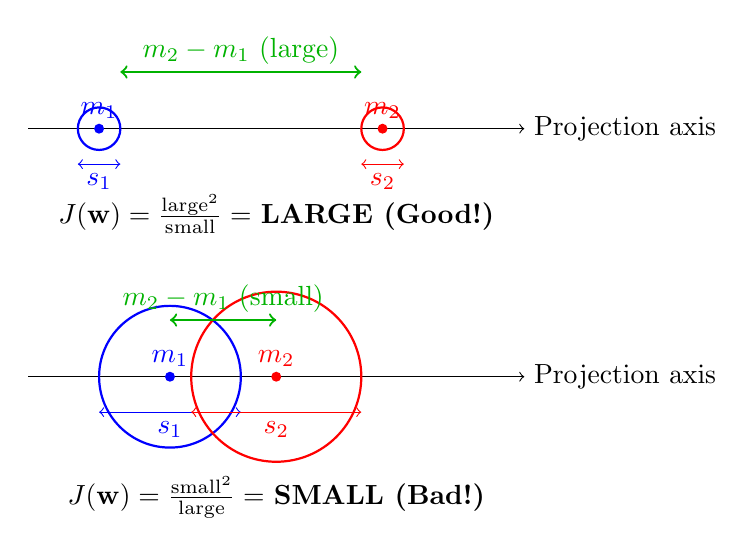
\begin{tikzpicture}[scale=0.9]
    % Good projection
    \begin{scope}
        \draw[->] (0,0) -- (7,0) node[right] {Projection axis};
        
        % Class 1
        \draw[blue, thick] (1,0) circle (0.3);
        \fill[blue] (1,0) circle (2pt) node[above] {$m_1$};
        \draw[<->, blue] (0.7, -0.5) -- (1.3, -0.5) node[midway, below] {$s_1$};
        
        % Class 2
        \draw[red, thick] (5,0) circle (0.3);
        \fill[red] (5,0) circle (2pt) node[above] {$m_2$};
        \draw[<->, red] (4.7, -0.5) -- (5.3, -0.5) node[midway, below] {$s_2$};
        
        % Between-class distance
        \draw[<->, thick, green!70!black] (1.3, 0.8) -- (4.7, 0.8);
        \node[green!70!black] at (3, 1.1) {$m_2 - m_1$ (large)};
        
        \node at (3.5, -1.2) {$J(\mathbf{w}) = \frac{\text{large}^2}{\text{small}} = $ \textbf{LARGE (Good!)}};
    \end{scope}
    
    % Bad projection
    \begin{scope}[shift={(0,-3.5)}]
        \draw[->] (0,0) -- (7,0) node[right] {Projection axis};
        
        % Class 1
        \draw[blue, thick] (2,0) circle (1.0);
        \fill[blue] (2,0) circle (2pt) node[above] {$m_1$};
        \draw[<->, blue] (1, -0.5) -- (3, -0.5) node[midway, below] {$s_1$};
        
        % Class 2
        \draw[red, thick] (3.5,0) circle (1.2);
        \fill[red] (3.5,0) circle (2pt) node[above] {$m_2$};
        \draw[<->, red] (2.3, -0.5) -- (4.7, -0.5) node[midway, below] {$s_2$};
        
        % Between-class distance
        \draw[<->, thick, green!70!black] (2, 0.8) -- (3.5, 0.8);
        \node[green!70!black] at (2.75, 1.1) {$m_2 - m_1$ (small)};
        
        \node at (3.5, -1.7) {$J(\mathbf{w}) = \frac{\text{small}^2}{\text{large}} = $ \textbf{SMALL (Bad!)}};
    \end{scope}
\end{tikzpicture}
\end{center}

\textbf{Good projection:} Large separation, small scatter → Large $J(\mathbf{w})$

\textbf{Bad projection:} Small separation, large scatter → Small $J(\mathbf{w})$
\end{geometrybox}

\section{The Solution: Optimal Direction}

\subsection{Scatter Matrices}

To derive the solution, we need to express everything in matrix form.

\begin{definition}[Within-Class Scatter Matrix]
For class $k$:
\begin{equation}
    \mathbf{S}_k = \sum_{i \in C_k} (\mathbf{x}_i - \boldsymbol{\mu}_k)(\mathbf{x}_i - \boldsymbol{\mu}_k)^T
\end{equation}

Total within-class scatter:
\begin{equation}
    \mathbf{S}_W = \mathbf{S}_1 + \mathbf{S}_2
\end{equation}

This is a $p \times p$ matrix measuring spread within classes.
\end{definition}

\begin{definition}[Between-Class Scatter Matrix]
\begin{equation}
    \mathbf{S}_B = (\boldsymbol{\mu}_1 - \boldsymbol{\mu}_2)(\boldsymbol{\mu}_1 - \boldsymbol{\mu}_2)^T
\end{equation}

This is a $p \times p$ matrix (rank 1) measuring separation between class means.
\end{definition}

\subsection{Fisher's Criterion in Matrix Form}

\begin{theorem}[Matrix Form of Fisher's Criterion]
The Fisher criterion can be written as:
\begin{equation}
    J(\mathbf{w}) = \frac{\mathbf{w}^T\mathbf{S}_B\mathbf{w}}{\mathbf{w}^T\mathbf{S}_W\mathbf{w}}
\end{equation}

This is a \textbf{Rayleigh quotient}.
\end{theorem}

\begin{proof}[Derivation]
\textbf{Numerator (between-class):}
\begin{align}
    (m_1 - m_2)^2 &= (\mathbf{w}^T(\boldsymbol{\mu}_1 - \boldsymbol{\mu}_2))^2 \\
    &= \mathbf{w}^T(\boldsymbol{\mu}_1 - \boldsymbol{\mu}_2)(\boldsymbol{\mu}_1 - \boldsymbol{\mu}_2)^T\mathbf{w} \\
    &= \mathbf{w}^T\mathbf{S}_B\mathbf{w}
\end{align}

\textbf{Denominator (within-class):}
\begin{align}
    s_k^2 &= \sum_{i \in C_k} (\mathbf{w}^T(\mathbf{x}_i - \boldsymbol{\mu}_k))^2 \\
    &= \sum_{i \in C_k} \mathbf{w}^T(\mathbf{x}_i - \boldsymbol{\mu}_k)(\mathbf{x}_i - \boldsymbol{\mu}_k)^T\mathbf{w} \\
    &= \mathbf{w}^T\mathbf{S}_k\mathbf{w}
\end{align}

Therefore:
\begin{equation}
    s_1^2 + s_2^2 = \mathbf{w}^T(\mathbf{S}_1 + \mathbf{S}_2)\mathbf{w} = \mathbf{w}^T\mathbf{S}_W\mathbf{w}
\end{equation}
\end{proof}

\subsection{The Optimal Solution}

\begin{theorem}[Fisher's LDA Solution]
The optimal direction $\mathbf{w}$ that maximizes $J(\mathbf{w})$ is:

\begin{equation}
    \boxed{\mathbf{w} \propto \mathbf{S}_W^{-1}(\boldsymbol{\mu}_1 - \boldsymbol{\mu}_2)}
\end{equation}

Since we only care about direction (not magnitude), we can write:
\begin{equation}
    \mathbf{w} = \mathbf{S}_W^{-1}(\boldsymbol{\mu}_1 - \boldsymbol{\mu}_2)
\end{equation}
\end{theorem}

\begin{proof}[Derivation]
To maximize $J(\mathbf{w}) = \frac{\mathbf{w}^T\mathbf{S}_B\mathbf{w}}{\mathbf{w}^T\mathbf{S}_W\mathbf{w}}$, we take the derivative and set to zero.

Using calculus of variations (or Lagrange multipliers), the solution satisfies:
\begin{equation}
    \mathbf{S}_B\mathbf{w} = \lambda \mathbf{S}_W\mathbf{w}
\end{equation}

This is a generalized eigenvalue problem.

Since $\mathbf{S}_B = (\boldsymbol{\mu}_1 - \boldsymbol{\mu}_2)(\boldsymbol{\mu}_1 - \boldsymbol{\mu}_2)^T$:
\begin{equation}
    \mathbf{S}_B\mathbf{w} = (\boldsymbol{\mu}_1 - \boldsymbol{\mu}_2)[(\boldsymbol{\mu}_1 - \boldsymbol{\mu}_2)^T\mathbf{w}]
\end{equation}

The term in brackets is a scalar, say $c$. So:
\begin{equation}
    \mathbf{S}_B\mathbf{w} = c(\boldsymbol{\mu}_1 - \boldsymbol{\mu}_2)
\end{equation}

Substituting into eigenvalue equation:
\begin{align}
    c(\boldsymbol{\mu}_1 - \boldsymbol{\mu}_2) &= \lambda \mathbf{S}_W\mathbf{w} \\
    \mathbf{w} &= \frac{c}{\lambda}\mathbf{S}_W^{-1}(\boldsymbol{\mu}_1 - \boldsymbol{\mu}_2)
\end{align}

Since we only care about direction, we can ignore the scalar $\frac{c}{\lambda}$:
\begin{equation}
    \mathbf{w} = \mathbf{S}_W^{-1}(\boldsymbol{\mu}_1 - \boldsymbol{\mu}_2)
\end{equation}
\end{proof}

\begin{keyidea}
\textbf{Beautiful insight:}

The optimal direction $\mathbf{w}$ is:
\begin{itemize}
    \item Proportional to the difference in class means: $(\boldsymbol{\mu}_1 - \boldsymbol{\mu}_2)$
    \item Adjusted by the inverse of within-class scatter: $\mathbf{S}_W^{-1}$
\end{itemize}

If classes had no internal scatter ($\mathbf{S}_W = \mathbf{I}$), the optimal direction would just be the line connecting the means!

The $\mathbf{S}_W^{-1}$ term adjusts for the shape and spread of each class.
\end{keyidea}

\section{Complete Numerical Example}

\begin{example}[2D LDA by Hand]

\textbf{Training data:} Two classes in 2D

\textbf{Class 1 (Blue):}
\begin{equation}
    \mathbf{x}_1 = \begin{bmatrix} 1 \\ 2 \end{bmatrix}, \quad
    \mathbf{x}_2 = \begin{bmatrix} 2 \\ 3 \end{bmatrix}, \quad
    \mathbf{x}_3 = \begin{bmatrix} 3 \\ 3 \end{bmatrix}
\end{equation}

\textbf{Class 2 (Red):}
\begin{equation}
    \mathbf{x}_4 = \begin{bmatrix} 6 \\ 5 \end{bmatrix}, \quad
    \mathbf{x}_5 = \begin{bmatrix} 7 \\ 6 \end{bmatrix}
\end{equation}

\textbf{STEP 1: Compute class means}

\textbf{Class 1 mean:}
\begin{equation}
    \boldsymbol{\mu}_1 = \frac{1}{3}\left(\begin{bmatrix} 1 \\ 2 \end{bmatrix} + \begin{bmatrix} 2 \\ 3 \end{bmatrix} + \begin{bmatrix} 3 \\ 3 \end{bmatrix}\right) = \frac{1}{3}\begin{bmatrix} 6 \\ 8 \end{bmatrix} = \begin{bmatrix} 2 \\ 2.67 \end{bmatrix}
\end{equation}

\textbf{Class 2 mean:}
\begin{equation}
    \boldsymbol{\mu}_2 = \frac{1}{2}\left(\begin{bmatrix} 6 \\ 5 \end{bmatrix} + \begin{bmatrix} 7 \\ 6 \end{bmatrix}\right) = \frac{1}{2}\begin{bmatrix} 13 \\ 11 \end{bmatrix} = \begin{bmatrix} 6.5 \\ 5.5 \end{bmatrix}
\end{equation}

\textbf{STEP 2: Compute within-class scatter matrices}

\textbf{For Class 1:}
\begin{align}
    \mathbf{x}_1 - \boldsymbol{\mu}_1 &= \begin{bmatrix} 1 \\ 2 \end{bmatrix} - \begin{bmatrix} 2 \\ 2.67 \end{bmatrix} = \begin{bmatrix} -1 \\ -0.67 \end{bmatrix} \\
    \mathbf{x}_2 - \boldsymbol{\mu}_1 &= \begin{bmatrix} 2 \\ 3 \end{bmatrix} - \begin{bmatrix} 2 \\ 2.67 \end{bmatrix} = \begin{bmatrix} 0 \\ 0.33 \end{bmatrix} \\
    \mathbf{x}_3 - \boldsymbol{\mu}_1 &= \begin{bmatrix} 3 \\ 3 \end{bmatrix} - \begin{bmatrix} 2 \\ 2.67 \end{bmatrix} = \begin{bmatrix} 1 \\ 0.33 \end{bmatrix}
\end{align}

\begin{align}
    \mathbf{S}_1 &= \sum_{i=1}^{3} (\mathbf{x}_i - \boldsymbol{\mu}_1)(\mathbf{x}_i - \boldsymbol{\mu}_1)^T \\
    &= \begin{bmatrix} -1 \\ -0.67 \end{bmatrix}\begin{bmatrix} -1 & -0.67 \end{bmatrix} + \begin{bmatrix} 0 \\ 0.33 \end{bmatrix}\begin{bmatrix} 0 & 0.33 \end{bmatrix} + \begin{bmatrix} 1 \\ 0.33 \end{bmatrix}\begin{bmatrix} 1 & 0.33 \end{bmatrix} \\
    &= \begin{bmatrix} 1 & 0.67 \\ 0.67 & 0.45 \end{bmatrix} + \begin{bmatrix} 0 & 0 \\ 0 & 0.11 \end{bmatrix} + \begin{bmatrix} 1 & 0.33 \\ 0.33 & 0.11 \end{bmatrix} \\
    &= \begin{bmatrix} 2 & 1 \\ 1 & 0.67 \end{bmatrix}
\end{align}

\textbf{For Class 2:}
\begin{align}
    \mathbf{x}_4 - \boldsymbol{\mu}_2 &= \begin{bmatrix} 6 \\ 5 \end{bmatrix} - \begin{bmatrix} 6.5 \\ 5.5 \end{bmatrix} = \begin{bmatrix} -0.5 \\ -0.5 \end{bmatrix} \\
    \mathbf{x}_5 - \boldsymbol{\mu}_2 &= \begin{bmatrix} 7 \\ 6 \end{bmatrix} - \begin{bmatrix} 6.5 \\ 5.5 \end{bmatrix} = \begin{bmatrix} 0.5 \\ 0.5 \end{bmatrix}
\end{align}

\begin{align}
    \mathbf{S}_2 &= \begin{bmatrix} -0.5 \\ -0.5 \end{bmatrix}\begin{bmatrix} -0.5 & -0.5 \end{bmatrix} + \begin{bmatrix} 0.5 \\ 0.5 \end{bmatrix}\begin{bmatrix} 0.5 & 0.5 \end{bmatrix} \\
    &= \begin{bmatrix} 0.25 & 0.25 \\ 0.25 & 0.25 \end{bmatrix} + \begin{bmatrix} 0.25 & 0.25 \\ 0.25 & 0.25 \end{bmatrix} \\
    &= \begin{bmatrix} 0.5 & 0.5 \\ 0.5 & 0.5 \end{bmatrix}
\end{align}

\textbf{Total within-class scatter:}
\begin{equation}
    \mathbf{S}_W = \mathbf{S}_1 + \mathbf{S}_2 = \begin{bmatrix} 2 & 1 \\ 1 & 0.67 \end{bmatrix} + \begin{bmatrix} 0.5 & 0.5 \\ 0.5 & 0.5 \end{bmatrix} = \begin{bmatrix} 2.5 & 1.5 \\ 1.5 & 1.17 \end{bmatrix}
\end{equation}

\textbf{STEP 3: Compute $\mathbf{S}_W^{-1}$}

For $2 \times 2$ matrix $\begin{bmatrix} a & b \\ c & d \end{bmatrix}$:
\begin{equation}
    \text{Inverse} = \frac{1}{ad - bc}\begin{bmatrix} d & -b \\ -c & a \end{bmatrix}
\end{equation}

\begin{align}
    \det(\mathbf{S}_W) &= 2.5(1.17) - 1.5(1.5) = 2.925 - 2.25 = 0.675
\end{align}

\begin{equation}
    \mathbf{S}_W^{-1} = \frac{1}{0.675}\begin{bmatrix} 1.17 & -1.5 \\ -1.5 & 2.5 \end{bmatrix} = \begin{bmatrix} 1.73 & -2.22 \\ -2.22 & 3.70 \end{bmatrix}
\end{equation}

\textbf{STEP 4: Compute difference in means}

\begin{equation}
    \boldsymbol{\mu}_1 - \boldsymbol{\mu}_2 = \begin{bmatrix} 2 \\ 2.67 \end{bmatrix} - \begin{bmatrix} 6.5 \\ 5.5 \end{bmatrix} = \begin{bmatrix} -4.5 \\ -2.83 \end{bmatrix}
\end{equation}

\textbf{STEP 5: Compute optimal direction $\mathbf{w}$}

\begin{align}
    \mathbf{w} &= \mathbf{S}_W^{-1}(\boldsymbol{\mu}_1 - \boldsymbol{\mu}_2) \\
    &= \begin{bmatrix} 1.73 & -2.22 \\ -2.22 & 3.70 \end{bmatrix}\begin{bmatrix} -4.5 \\ -2.83 \end{bmatrix} \\
    &= \begin{bmatrix} 1.73(-4.5) + (-2.22)(-2.83) \\ -2.22(-4.5) + 3.70(-2.83) \end{bmatrix} \\
    &= \begin{bmatrix} -7.785 + 6.283 \\ 9.99 - 10.471 \end{bmatrix} \\
    &= \begin{bmatrix} -1.502 \\ -0.481 \end{bmatrix}
\end{align}

We can normalize (optional):
\begin{equation}
    ||\mathbf{w}|| = \sqrt{(-1.502)^2 + (-0.481)^2} = \sqrt{2.256 + 0.231} = \sqrt{2.487} \approx 1.577
\end{equation}

\begin{equation}
    \mathbf{w}_{\text{normalized}} = \frac{1}{1.577}\begin{bmatrix} -1.502 \\ -0.481 \end{bmatrix} \approx \begin{bmatrix} -0.952 \\ -0.305 \end{bmatrix}
\end{equation}

\textbf{STEP 6: Project data onto $\mathbf{w}$}

For each point, compute $y = \mathbf{w}^T\mathbf{x}$:

\textbf{Class 1:}
\begin{align}
    y_1 &= \begin{bmatrix} -1.502 & -0.481 \end{bmatrix}\begin{bmatrix} 1 \\ 2 \end{bmatrix} = -1.502 - 0.962 = -2.464 \\
    y_2 &= \begin{bmatrix} -1.502 & -0.481 \end{bmatrix}\begin{bmatrix} 2 \\ 3 \end{bmatrix} = -3.004 - 1.443 = -4.447 \\
    y_3 &= \begin{bmatrix} -1.502 & -0.481 \end{bmatrix}\begin{bmatrix} 3 \\ 3 \end{bmatrix} = -4.506 - 1.443 = -5.949
\end{align}

\textbf{Class 2:}
\begin{align}
    y_4 &= \begin{bmatrix} -1.502 & -0.481 \end{bmatrix}\begin{bmatrix} 6 \\ 5 \end{bmatrix} = -9.012 - 2.405 = -11.417 \\
    y_5 &= \begin{bmatrix} -1.502 & -0.481 \end{bmatrix}\begin{bmatrix} 7 \\ 6 \end{bmatrix} = -10.514 - 2.886 = -13.400
\end{align}

\textbf{STEP 7: Classification}

Compute projected class means:
\begin{align}
    m_1 &= \frac{-2.464 + (-4.447) + (-5.949)}{3} = \frac{-12.86}{3} = -4.287 \\
    m_2 &= \frac{-11.417 + (-13.400)}{2} = \frac{-24.817}{2} = -12.409
\end{align}

Decision boundary (midpoint):
\begin{equation}
    \text{threshold} = \frac{m_1 + m_2}{2} = \frac{-4.287 + (-12.409)}{2} = \frac{-16.696}{2} = -8.348
\end{equation}

\textbf{Classification rule:}
\begin{equation}
    \text{Classify as } \begin{cases}
        \text{Class 1} & \text{if } y > -8.348 \\
        \text{Class 2} & \text{if } y < -8.348
    \end{cases}
\end{equation}

\textbf{Verify:} All class 1 points have $y > -8.348$, all class 2 points have $y < -8.348$ → Perfect separation!
\end{example}

\section{LDA as a Generative Model}

\subsection{Probabilistic Interpretation}

\begin{definition}[Gaussian Class-Conditional Densities]
LDA assumes each class has a Gaussian distribution:
\begin{equation}
    P(\mathbf{x}|y=C_k) = \mathcal{N}(\mathbf{x}|\boldsymbol{\mu}_k, \boldsymbol{\Sigma})
\end{equation}

\textbf{Key assumption:} All classes share the \textbf{same covariance matrix} $\boldsymbol{\Sigma}$.

(If covariances differ, we get Quadratic Discriminant Analysis (QDA) instead.)
\end{definition}

\begin{theorem}[LDA Decision Boundary is Linear]
With equal covariance matrices, the decision boundary between classes is:
\begin{equation}
    \log\frac{P(y=C_1|\mathbf{x})}{P(y=C_2|\mathbf{x})} = \mathbf{w}^T\mathbf{x} + w_0 = 0
\end{equation}

where:
\begin{align}
    \mathbf{w} &= \boldsymbol{\Sigma}^{-1}(\boldsymbol{\mu}_1 - \boldsymbol{\mu}_2) \\
    w_0 &= \text{constant involving priors and means}
\end{align}

This is a \textbf{hyperplane} in feature space!
\end{theorem}

\begin{note}
In practice:
\begin{itemize}
    \item $\boldsymbol{\mu}_k$ estimated by sample means
    \item $\boldsymbol{\Sigma}$ estimated by pooled covariance: $\hat{\boldsymbol{\Sigma}} = \frac{\mathbf{S}_W}{n-K}$
\end{itemize}
\end{note}

\section{Multi-Class LDA}

\begin{definition}[LDA for $K > 2$ Classes]
With $K$ classes:
\begin{itemize}
    \item Within-class scatter: $\mathbf{S}_W = \sum_{k=1}^{K}\sum_{i \in C_k}(\mathbf{x}_i - \boldsymbol{\mu}_k)(\mathbf{x}_i - \boldsymbol{\mu}_k)^T$
    \item Between-class scatter: $\mathbf{S}_B = \sum_{k=1}^{K}n_k(\boldsymbol{\mu}_k - \boldsymbol{\mu})(\boldsymbol{\mu}_k - \boldsymbol{\mu})^T$
\end{itemize}

where $\boldsymbol{\mu} = \frac{1}{n}\sum_{k=1}^{K}n_k\boldsymbol{\mu}_k$ is the overall mean.

Find $K-1$ orthogonal directions (discriminants) that maximize:
\begin{equation}
    J(\mathbf{W}) = \frac{|\mathbf{W}^T\mathbf{S}_B\mathbf{W}|}{|\mathbf{W}^T\mathbf{S}_W\mathbf{W}|}
\end{equation}

\textbf{Solution:} Eigenvectors of $\mathbf{S}_W^{-1}\mathbf{S}_B$ corresponding to largest eigenvalues.
\end{definition}

\begin{keyidea}
With $K$ classes in $p$ dimensions, LDA finds at most $\min(K-1, p)$ discriminant directions.

\textbf{Dimensionality reduction:} Project $p$-dimensional data onto $(K-1)$-dimensional space!

Example: 1000 features, 3 classes → LDA reduces to 2 dimensions while preserving class separation.
\end{keyidea}

\section{LDA vs Other Methods}

\begin{importantbox}
\textbf{LDA vs Logistic Regression:}
\begin{itemize}
    \item \textbf{LDA:} Generative (models $P(\mathbf{x}|y)$, assumes Gaussian)
    \item \textbf{Logistic:} Discriminative (models $P(y|\mathbf{x})$ directly)
    \item \textbf{LDA:} More efficient when assumptions hold; closed-form solution
    \item \textbf{Logistic:} More robust when assumptions violated; iterative
\end{itemize}

\textbf{LDA vs Naive Bayes:}
\begin{itemize}
    \item \textbf{LDA:} Assumes features correlated (full covariance)
    \item \textbf{NB:} Assumes features independent (diagonal covariance)
    \item \textbf{LDA:} Needs more data to estimate covariance
    \item \textbf{NB:} Works better with limited data, high dimensions
\end{itemize}

\textbf{LDA vs PCA (dimensionality reduction):}
\begin{itemize}
    \item \textbf{LDA:} Supervised (uses class labels), maximizes class separation
    \item \textbf{PCA:} Unsupervised (ignores labels), maximizes variance
    \item \textbf{LDA:} Best for classification tasks
    \item \textbf{PCA:} Best for exploratory data analysis
\end{itemize}
\end{importantbox}

\section{Assumptions and Limitations}

\begin{definition}[LDA Assumptions]
\begin{enumerate}
    \item \textbf{Gaussian distributions:} Each class follows multivariate normal
    \item \textbf{Equal covariance:} All classes have same covariance matrix $\boldsymbol{\Sigma}$
    \item \textbf{Linear separability:} Classes can be separated by hyperplane
\end{enumerate}

\textbf{When violated:}
\begin{itemize}
    \item Non-Gaussian data → Consider non-parametric methods (k-NN, SVM)
    \item Unequal covariance → Use QDA instead
    \item Non-linear separation → Use kernel methods, neural networks
\end{itemize}
\end{definition}

\begin{keyidea}
\textbf{Advantages:}
\begin{enumerate}
    \item Simple, interpretable
    \item Closed-form solution (no iteration)
    \item Fast training and prediction
    \item Works well when assumptions hold
    \item Natural dimensionality reduction
    \item Handles multi-class natively
\end{enumerate}

\textbf{Disadvantages:}
\begin{enumerate}
    \item Strong distributional assumptions
    \item Assumes equal covariance (restrictive)
    \item Linear decision boundaries only
    \item Sensitive to outliers
    \item Needs $\mathbf{S}_W$ to be invertible (requires $n > p$)
    \item Poor performance when assumptions violated
\end{enumerate}
\end{keyidea}

\section{GATE-Style Problems}

\begin{example}[Problem 1: Simple 1D LDA]

\textbf{Given:}
\begin{itemize}
    \item Class 1: $x = \{1, 2, 3\}$, mean $\mu_1 = 2$, variance $s_1^2 = 1$
    \item Class 2: $x = \{7, 8, 9\}$, mean $\mu_2 = 8$, variance $s_2^2 = 1$
\end{itemize}

\textbf{Find the LDA decision boundary.}

\textbf{Solution:}

In 1D, $\mathbf{w}$ is just a scalar (direction: positive or negative).

\textbf{Between-class separation:}
\begin{equation}
    (\mu_1 - \mu_2)^2 = (2 - 8)^2 = 36
\end{equation}

\textbf{Within-class scatter:}
\begin{equation}
    s_1^2 + s_2^2 = 1 + 1 = 2
\end{equation}

\textbf{Fisher criterion:}
\begin{equation}
    J = \frac{36}{2} = 18
\end{equation}

\textbf{Decision boundary:} Midpoint between means
\begin{equation}
    \text{threshold} = \frac{\mu_1 + \mu_2}{2} = \frac{2 + 8}{2} = 5
\end{equation}

\textbf{Classification:} Class 1 if $x < 5$, Class 2 if $x > 5$
\end{example}

\begin{example}[Problem 2: Computing $\mathbf{w}$ for 2D Data]

\textbf{Given:}
\begin{align}
    \boldsymbol{\mu}_1 &= \begin{bmatrix} 0 \\ 0 \end{bmatrix}, \quad
    \boldsymbol{\mu}_2 = \begin{bmatrix} 2 \\ 2 \end{bmatrix} \\
    \mathbf{S}_W &= \begin{bmatrix} 1 & 0 \\ 0 & 1 \end{bmatrix} = \mathbf{I}
\end{align}

\textbf{Find the discriminant direction $\mathbf{w}$.}

\textbf{Solution:}

\begin{align}
    \mathbf{w} &= \mathbf{S}_W^{-1}(\boldsymbol{\mu}_1 - \boldsymbol{\mu}_2) \\
    &= \mathbf{I}^{-1}\left(\begin{bmatrix} 0 \\ 0 \end{bmatrix} - \begin{bmatrix} 2 \\ 2 \end{bmatrix}\right) \\
    &= \begin{bmatrix} -2 \\ -2 \end{bmatrix}
\end{align}

Direction: $\mathbf{w} \propto \begin{bmatrix} 1 \\ 1 \end{bmatrix}$ (normalized)

\textbf{Interpretation:} The discriminant is the line $y = x$ (45° angle).
\end{example}

\begin{example}[Problem 3: Fisher Criterion Calculation]

\textbf{Question:} Two projections give:
\begin{itemize}
    \item Projection A: $m_1 = 2, m_2 = 8, s_1^2 = 1, s_2^2 = 1$
    \item Projection B: $m_1 = 3, m_2 = 7, s_1^2 = 4, s_2^2 = 4$
\end{itemize}

Which projection is better according to Fisher's criterion?

\textbf{Solution:}

\textbf{Projection A:}
\begin{equation}
    J_A = \frac{(8-2)^2}{1+1} = \frac{36}{2} = 18
\end{equation}

\textbf{Projection B:}
\begin{equation}
    J_B = \frac{(7-3)^2}{4+4} = \frac{16}{8} = 2
\end{equation}

Since $18 > 2$: \textbf{Projection A is better}

Despite having same separation of means (distance 6 vs 4), Projection A has much tighter clusters.
\end{example}

\section{Summary - Key Points for GATE}

\begin{importantbox}
\textbf{Must Know for GATE:}

\begin{enumerate}
    \item \textbf{Goal:} Find projection that maximizes class separation while minimizing within-class scatter
    
    \item \textbf{Fisher's criterion:}
    \begin{equation}
        J(\mathbf{w}) = \frac{(m_1 - m_2)^2}{s_1^2 + s_2^2} = \frac{\mathbf{w}^T\mathbf{S}_B\mathbf{w}}{\mathbf{w}^T\mathbf{S}_W\mathbf{w}}
    \end{equation}
    
    \item \textbf{Optimal direction:}
    \begin{equation}
        \mathbf{w} = \mathbf{S}_W^{-1}(\boldsymbol{\mu}_1 - \boldsymbol{\mu}_2)
    \end{equation}
    
    \item \textbf{Scatter matrices:}
    \begin{align}
        \mathbf{S}_W &= \sum_{k}\sum_{i \in C_k}(\mathbf{x}_i - \boldsymbol{\mu}_k)(\mathbf{x}_i - \boldsymbol{\mu}_k)^T \\
        \mathbf{S}_B &= \sum_{k}n_k(\boldsymbol{\mu}_k - \boldsymbol{\mu})(\boldsymbol{\mu}_k - \boldsymbol{\mu})^T
    \end{align}
    
    \item \textbf{Assumptions:}
    \begin{itemize}
        \item Gaussian class distributions
        \item Equal covariance matrices
        \item Linear separability
    \end{itemize}
    
    \item \textbf{Multi-class:} Find $K-1$ discriminants (dimensionality reduction)
    
    \item \textbf{Decision boundary:} Hyperplane in original space, threshold in projected space
    
    \item \textbf{Complexity:} $O(p^3)$ for matrix inversion, $O(np^2)$ for scatter matrices
    
    \item \textbf{vs Logistic:} Generative vs discriminative
    
    \item \textbf{vs PCA:} Supervised (uses labels) vs unsupervised
    
    \item \textbf{vs QDA:} Equal covariance vs different covariances → linear vs quadratic boundary
\end{enumerate}
\end{importantbox}

\begin{gatepoint}
\textbf{Common GATE Question Types:}

\begin{enumerate}
    \item Compute Fisher's criterion for given projections
    \item Calculate $\mathbf{w}$ from means and scatter matrices
    \item Compute scatter matrices from data
    \item Understand geometric interpretation of LDA
    \item Compare LDA with other classifiers
    \item Know assumptions and when they're violated
    \item Understand dimensionality reduction aspect
    \item Compute decision boundary
    \item Know complexity and computational requirements
    \item Explain why equal covariance leads to linear boundary
\end{enumerate}
\end{gatepoint}
\chapter{Support Vector Machine (SVM): Maximum Margin Classification}

\section{Introduction to SVM}

\begin{mentalmodel}
Imagine you're a referee trying to draw a line to separate two teams on a field. There are many possible lines you could draw. Which one is best?

\textbf{Intuition:} Draw the line that is as far as possible from both teams!

This gives you the most "safety margin" - if players move a bit, they're still on the correct side.

\textbf{This is exactly what SVM does!}
\end{mentalmodel}

\begin{keyidea}
Support Vector Machine (SVM) is a powerful classification algorithm with a beautiful geometric interpretation:

\textbf{Core principle:} Among all possible decision boundaries that separate the classes, choose the one with the \textbf{maximum margin}.

\textbf{Margin:} The distance from the decision boundary to the nearest data point from either class.

\textbf{Support vectors:} The data points closest to the decision boundary (they "support" or define it).
\end{keyidea}

\section{The Maximum Margin Concept}

\subsection{What is a Margin?}

\begin{definition}[Margin]
For a linear classifier with decision boundary $\mathbf{w}^T\mathbf{x} + b = 0$:

The \textbf{margin} is the perpendicular distance from the decision boundary to the closest data point.

\textbf{Maximum margin classifier:} The classifier that maximizes this margin.
\end{definition}

\begin{geometrybox}
\textbf{Visualizing Different Decision Boundaries:}

\begin{center}
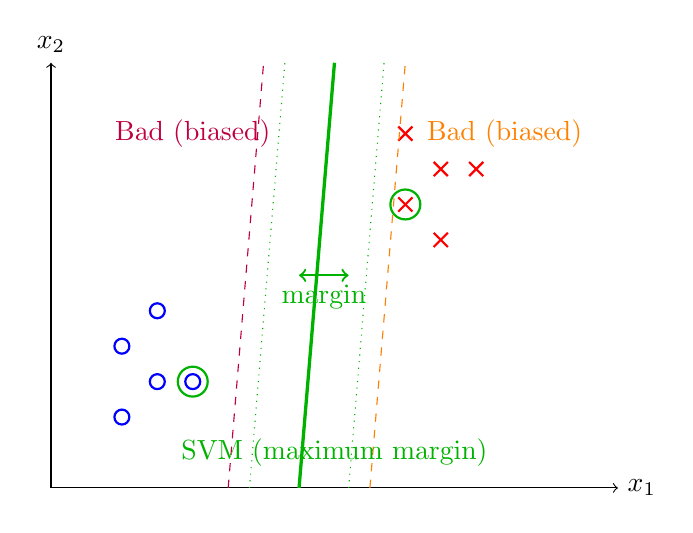
\begin{tikzpicture}[scale=0.9]
    % Setup
    \draw[->] (0,0) -- (8,0) node[right] {$x_1$};
    \draw[->] (0,0) -- (0,6) node[above] {$x_2$};
    
    % Class 1 points (blue circles)
    \foreach \x/\y in {1/1, 1.5/1.5, 1/2, 1.5/2.5, 2/1.5} {
        \draw[blue, thick] (\x,\y) circle (3pt);
    }
    
    % Class 2 points (red crosses)
    \foreach \x/\y in {5/4, 5.5/4.5, 5/5, 6/4.5, 5.5/3.5} {
        \draw[red, thick] (\x-0.1,\y-0.1) -- (\x+0.1,\y+0.1);
        \draw[red, thick] (\x-0.1,\y+0.1) -- (\x+0.1,\y-0.1);
    }
    
    % Bad boundary 1 (too close to class 1)
    \draw[purple, dashed] (2.5,0) -- (3,6);
    \node[purple] at (2,5) {Bad (biased)};
    
    % Bad boundary 2 (too close to class 2)  
    \draw[orange, dashed] (4.5,0) -- (5,6);
    \node[orange] at (6.4,5) {Bad (biased)};
    
    % Good boundary (maximum margin)
    \draw[green!70!black, very thick] (3.5,0) -- (4,6);
    
    % Margin lines
    \draw[green!70!black, dotted] (2.8,0) -- (3.3,6);
    \draw[green!70!black, dotted] (4.2,0) -- (4.7,6);
    
    % Margin annotation
    \draw[<->, thick, green!70!black] (3.5,3) -- (4.2,3);
    \node[green!70!black, below] at (3.85,3) {margin};
    
    % Support vectors (circled)
    \draw[green!70!black, thick] (2,1.5) circle (6pt);
    \draw[green!70!black, thick] (5,4) circle (6pt);
    
    \node[green!70!black] at (4, 0.5) {SVM (maximum margin)};
\end{tikzpicture}
\end{center}

\textbf{Key insight:} Purple and orange lines separate classes but are risky - small perturbations could cause misclassification. The green line (SVM) has maximum "safety zone."
\end{geometrybox}

\subsection{Why Maximum Margin?}

\begin{importantbox}
\textbf{Why is maximum margin desirable?}

\begin{enumerate}
    \item \textbf{Robustness:} Less sensitive to small perturbations in data
    \item \textbf{Generalization:} Better performance on unseen data (lower overfitting)
    \item \textbf{Uniqueness:} Maximum margin solution is unique (unlike many possible separating hyperplanes)
    \item \textbf{Statistical justification:} Related to minimizing generalization error bounds (VC theory)
\end{enumerate}
\end{importantbox}

\section{Linear SVM: Hard Margin}

\subsection{Mathematical Setup}

\begin{definition}[Linear Separability]
A dataset is \textbf{linearly separable} if there exists a hyperplane that perfectly separates the two classes.

For binary classification with labels $y_i \in \{-1, +1\}$:

\begin{equation}
    \mathbf{w}^T\mathbf{x}_i + b > 0 \quad \text{for all } y_i = +1
\end{equation}
\begin{equation}
    \mathbf{w}^T\mathbf{x}_i + b < 0 \quad \text{for all } y_i = -1
\end{equation}

Combined:
\begin{equation}
    y_i(\mathbf{w}^T\mathbf{x}_i + b) > 0 \quad \text{for all } i
\end{equation}
\end{definition}

\begin{note}
\textbf{Why labels $\{-1, +1\}$ instead of $\{0, 1\}$?}

This makes the math cleaner! With $y_i \in \{-1, +1\}$:
\begin{itemize}
    \item Correct classification: $y_i(\mathbf{w}^T\mathbf{x}_i + b) > 0$
    \item Misclassification: $y_i(\mathbf{w}^T\mathbf{x}_i + b) < 0$
\end{itemize}

The sign naturally indicates correctness!
\end{note}

\subsection{Geometric Distance to Hyperplane}

\begin{theorem}[Distance from Point to Hyperplane]
The perpendicular distance from point $\mathbf{x}_0$ to hyperplane $\mathbf{w}^T\mathbf{x} + b = 0$ is:

\begin{equation}
    \text{distance} = \frac{|\mathbf{w}^T\mathbf{x}_0 + b|}{||\mathbf{w}||}
\end{equation}

where $||\mathbf{w}|| = \sqrt{\mathbf{w}^T\mathbf{w}}$ is the Euclidean norm.
\end{theorem}

\begin{proof}[Geometric Derivation]
The hyperplane $\mathbf{w}^T\mathbf{x} + b = 0$ can be written as:
\begin{equation}
    \mathbf{w}^T(\mathbf{x} - \mathbf{x}_0) = -(\mathbf{w}^T\mathbf{x}_0 + b)
\end{equation}

The vector $\mathbf{w}$ is perpendicular to the hyperplane.

The unit normal vector is: $\frac{\mathbf{w}}{||\mathbf{w}||}$

The signed distance from $\mathbf{x}_0$ to the plane is the projection of $(\mathbf{x}_0 - \mathbf{x}_{\text{plane}})$ onto the normal:

\begin{equation}
    d = \frac{\mathbf{w}^T\mathbf{x}_0 + b}{||\mathbf{w}||}
\end{equation}

The unsigned distance is the absolute value.
\end{proof}

\begin{example}[Computing Distance]
\textbf{Hyperplane:} $2x_1 + 3x_2 - 6 = 0$ (so $\mathbf{w} = [2, 3]^T$, $b = -6$)

\textbf{Point:} $\mathbf{x}_0 = [4, 5]^T$

\textbf{Distance:}
\begin{align}
    d &= \frac{|2(4) + 3(5) - 6|}{\sqrt{2^2 + 3^2}} \\
    &= \frac{|8 + 15 - 6|}{\sqrt{4 + 9}} \\
    &= \frac{17}{\sqrt{13}} \\
    &\approx \frac{17}{3.606} \approx 4.71
\end{align}
\end{example}

\subsection{The Margin}

\begin{definition}[Functional and Geometric Margin]

\textbf{Functional margin} of point $(\mathbf{x}_i, y_i)$:
\begin{equation}
    \hat{\gamma}_i = y_i(\mathbf{w}^T\mathbf{x}_i + b)
\end{equation}

\textbf{Geometric margin} of point $(\mathbf{x}_i, y_i)$:
\begin{equation}
    \gamma_i = y_i\frac{\mathbf{w}^T\mathbf{x}_i + b}{||\mathbf{w}||} = \frac{\hat{\gamma}_i}{||\mathbf{w}||}
\end{equation}

\textbf{Margin of the dataset:}
\begin{equation}
    \gamma = \min_{i=1,\ldots,n} \gamma_i
\end{equation}

The margin is the distance to the \textbf{closest} point.
\end{definition}

\begin{mentalmodel}
\textbf{Functional margin} can be made arbitrarily large by scaling $\mathbf{w}$ and $b$ (without changing the hyperplane).

Example: $2x_1 + 3x_2 - 6 = 0$ is the same as $4x_1 + 6x_2 - 12 = 0$

\textbf{Geometric margin} is scale-invariant - it's the actual perpendicular distance.

This is why we optimize the geometric margin!
\end{mentalmodel}

\section{SVM Optimization Problem}

\subsection{Canonical Form}

\begin{definition}[Canonical Hyperplane]
We can always scale $\mathbf{w}$ and $b$ such that the functional margin of the closest point(s) equals 1:

\begin{equation}
    \min_{i} y_i(\mathbf{w}^T\mathbf{x}_i + b) = 1
\end{equation}

This is called the \textbf{canonical form}.

With this scaling:
\begin{itemize}
    \item Points on the margin satisfy: $y_i(\mathbf{w}^T\mathbf{x}_i + b) = 1$
    \item All other points satisfy: $y_i(\mathbf{w}^T\mathbf{x}_i + b) \geq 1$
\end{itemize}
\end{definition}
\pagebreak
\begin{geometrybox}
\textbf{The SVM Geometry:}

\begin{center}
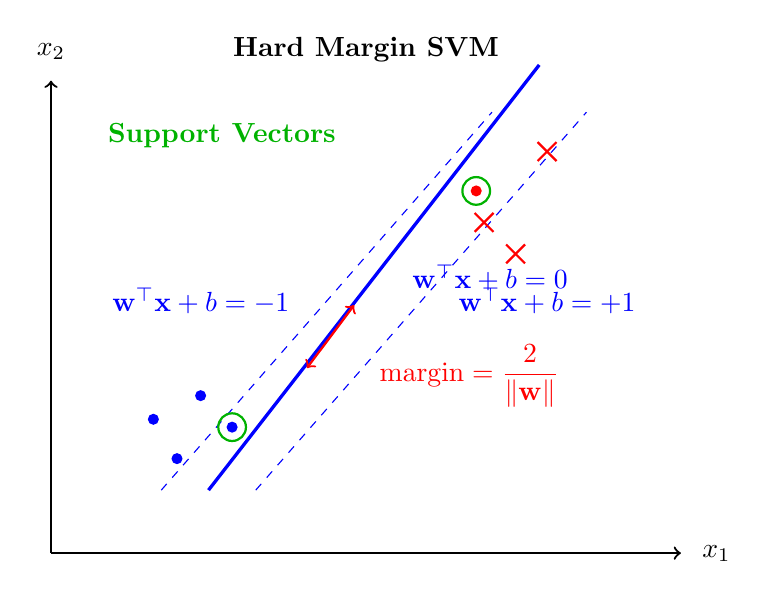
\begin{tikzpicture}[scale=1.0]

% =====================
% Axes
% =====================
\draw[->, thick] (0,0) -- (8,0) node[right=4pt] {$x_1$};
\draw[->, thick] (0,0) -- (0,6) node[above=4pt] {$x_2$};

% =====================
% Decision boundary
% =====================
\draw[very thick, blue]
    (2,0.8) -- (6.2,6.2)
    node[midway, right=10pt]
    {$\mathbf{w}^\top \mathbf{x} + b = 0$};

% =====================
% Margin boundaries
% =====================
\draw[dashed, blue]
    (1.4,0.8) -- (5.6,5.6)
    node[midway, left=10pt]
    {$\mathbf{w}^\top \mathbf{x} + b = -1$};

\draw[dashed, blue]
    (2.6,0.8) -- (6.8,5.6)
    node[midway, right=10pt]
    {$\mathbf{w}^\top \mathbf{x} + b = +1$};

% Margin (PERPENDICULAR)
% Direction vector perpendicular to the boundary
% (chosen consistent with boundary slope)
\coordinate (m1) at (3.25,2.35);   % on w^T x + b = -1
\coordinate (m2) at (3.85,3.15);   % on w^T x + b = +1

\draw[<->, thick, red] (m1) -- (m2);

\node[red, anchor=west]
  at ($(m2)+(0.2,-0.9)$)
  {$\text{margin}=\dfrac{2}{\lVert\mathbf{w}\rVert}$};

% =====================
% Class -1 points (blue dots)
% =====================
\fill[blue] (1.6,1.2) circle (2pt);
\fill[blue] (1.9,2.0) circle (2pt);
\fill[blue] (1.3,1.7) circle (2pt);

% Support vector (-1)
\fill[blue] (2.3,1.6) circle (2pt);
\draw[green!70!black, thick] (2.3,1.6) circle (5pt);

% =====================
% Class +1 points (red crosses)
% =====================
\foreach \x/\y in {5.5/4.2, 6.3/5.1, 5.9/3.8} {
    \draw[red, thick] (\x-0.12,\y-0.12) -- (\x+0.12,\y+0.12);
    \draw[red, thick] (\x-0.12,\y+0.12) -- (\x+0.12,\y-0.12);
}

% Support vector (+1)
\fill[red] (5.4,4.6) circle (2pt);
\draw[green!70!black, thick] (5.4,4.6) circle (5pt);

% =====================
% Annotations
% =====================
\node[green!70!black, anchor=west]
    at (0.6,5.3)
    {\textbf{Support Vectors}};

\node[font=\bfseries]
    at (4,6.4)
    {Hard Margin SVM};

\end{tikzpicture}
\end{center}

The margin width is $\frac{2}{||\mathbf{w}||}$ (distance between the two dashed lines).

Support vectors (circled) lie exactly on the margin boundaries.
\end{geometrybox}

\subsection{Margin Width}

\begin{theorem}[Width of the Margin]
In canonical form, the margin width is:
\begin{equation}
    \text{margin width} = \frac{2}{||\mathbf{w}||}
\end{equation}
\end{theorem}

\begin{proof}
Consider two points on opposite margin boundaries:
\begin{itemize}
    \item Point $\mathbf{x}_+$ on $\mathbf{w}^T\mathbf{x} + b = +1$ (class +1 side)
    \item Point $\mathbf{x}_-$ on $\mathbf{w}^T\mathbf{x} + b = -1$ (class -1 side)
\end{itemize}

The perpendicular distance from origin to each boundary:
\begin{align}
    d_+ &= \frac{1 - b}{||\mathbf{w}||} \\
    d_- &= \frac{-1 - b}{||\mathbf{w}||} = -\frac{1 + b}{||\mathbf{w}||}
\end{align}

The margin width:
\begin{align}
    \text{width} &= d_+ - d_- \\
    &= \frac{1 - b}{||\mathbf{w}||} - \left(-\frac{1 + b}{||\mathbf{w}||}\right) \\
    &= \frac{1 - b + 1 + b}{||\mathbf{w}||} \\
    &= \frac{2}{||\mathbf{w}||}
\end{align}
\end{proof}

\subsection{The Optimization Problem}

\begin{theorem}[Hard Margin SVM (Primal Form)]
\textbf{Maximize margin} is equivalent to:

\begin{equation}
    \boxed{
    \begin{aligned}
        \min_{\mathbf{w}, b} \quad & \frac{1}{2}||\mathbf{w}||^2 \\
        \text{subject to} \quad & y_i(\mathbf{w}^T\mathbf{x}_i + b) \geq 1, \quad i = 1, \ldots, n
    \end{aligned}
    }
\end{equation}

\textbf{Explanation:}
\begin{itemize}
    \item \textbf{Objective:} Minimize $\frac{1}{2}||\mathbf{w}||^2$ (maximize $\frac{2}{||\mathbf{w}||}$)
    \item \textbf{Constraints:} All points correctly classified with margin $\geq 1$
    \item Factor $\frac{1}{2}$ is for mathematical convenience (makes derivatives nicer)
    \item This is a \textbf{convex quadratic programming} problem!
\end{itemize}
\end{theorem}

\begin{keyidea}
\textbf{Why this formulation is beautiful:}

\begin{enumerate}
    \item \textbf{Convex:} One global minimum, no local minima
    \item \textbf{Quadratic objective:} $\frac{1}{2}||\mathbf{w}||^2$ is quadratic in $\mathbf{w}$
    \item \textbf{Linear constraints:} $y_i(\mathbf{w}^T\mathbf{x}_i + b) \geq 1$ are linear
    \item \textbf{Efficient algorithms:} Can be solved efficiently even for large $n$
    \item \textbf{Unique solution:} Maximum margin hyperplane is unique
\end{enumerate}
\end{keyidea}

\section{Dual Formulation and Support Vectors}

\subsection{Lagrangian Dual}

\begin{definition}[Lagrangian]
Introduce Lagrange multipliers $\alpha_i \geq 0$ for each constraint:

\begin{equation}
    \mathcal{L}(\mathbf{w}, b, \boldsymbol{\alpha}) = \frac{1}{2}||\mathbf{w}||^2 - \sum_{i=1}^{n}\alpha_i[y_i(\mathbf{w}^T\mathbf{x}_i + b) - 1]
\end{equation}

where $\boldsymbol{\alpha} = [\alpha_1, \ldots, \alpha_n]^T$.
\end{definition}

\begin{theorem}[KKT Conditions]
At the optimum, the Karush-Kuhn-Tucker (KKT) conditions hold:

\begin{align}
    \frac{\partial \mathcal{L}}{\partial \mathbf{w}} &= \mathbf{w} - \sum_{i=1}^{n}\alpha_i y_i \mathbf{x}_i = 0 \quad \Rightarrow \quad \boxed{\mathbf{w} = \sum_{i=1}^{n}\alpha_i y_i \mathbf{x}_i} \\
    \frac{\partial \mathcal{L}}{\partial b} &= -\sum_{i=1}^{n}\alpha_i y_i = 0 \quad \Rightarrow \quad \boxed{\sum_{i=1}^{n}\alpha_i y_i = 0} \\
    \alpha_i &\geq 0 \quad \text{for all } i \\
    y_i(\mathbf{w}^T\mathbf{x}_i + b) - 1 &\geq 0 \quad \text{for all } i \\
    \alpha_i[y_i(\mathbf{w}^T\mathbf{x}_i + b) - 1] &= 0 \quad \text{for all } i \quad \text{(complementary slackness)}
\end{align}
\end{theorem}

\begin{keyidea}
\textbf{The complementary slackness condition is crucial:}

\begin{equation}
    \alpha_i[y_i(\mathbf{w}^T\mathbf{x}_i + b) - 1] = 0
\end{equation}

This means for each point, either:
\begin{enumerate}
    \item $\alpha_i = 0$ (point is not on the margin), OR
    \item $y_i(\mathbf{w}^T\mathbf{x}_i + b) = 1$ (point is exactly on the margin)
\end{enumerate}

\textbf{Support vectors:} Points with $\alpha_i > 0$ (lie on the margin).

\textbf{Non-support vectors:} Points with $\alpha_i = 0$ (don't contribute to $\mathbf{w}$).
\end{keyidea}

\subsection{Dual Optimization Problem}

\begin{theorem}[Hard Margin SVM (Dual Form)]
Substituting the KKT conditions into the Lagrangian:

\begin{equation}
    \boxed{
    \begin{aligned}
        \max_{\boldsymbol{\alpha}} \quad & \sum_{i=1}^{n}\alpha_i - \frac{1}{2}\sum_{i=1}^{n}\sum_{j=1}^{n}\alpha_i\alpha_j y_i y_j \mathbf{x}_i^T\mathbf{x}_j \\
        \text{subject to} \quad & \alpha_i \geq 0, \quad i = 1, \ldots, n \\
        & \sum_{i=1}^{n}\alpha_i y_i = 0
    \end{aligned}
    }
\end{equation}

\textbf{Key observation:} The dual depends only on inner products $\mathbf{x}_i^T\mathbf{x}_j$!

This is the foundation for the kernel trick.
\end{theorem}

\subsection{Support Vectors}

\begin{definition}[Support Vectors]
The \textbf{support vectors} are training points with $\alpha_i > 0$.

These are exactly the points lying on the margin boundaries:
\begin{equation}
    y_i(\mathbf{w}^T\mathbf{x}_i + b) = 1
\end{equation}

\textbf{Critical properties:}
\begin{enumerate}
    \item Only support vectors contribute to $\mathbf{w} = \sum_{i}\alpha_i y_i \mathbf{x}_i$
    \item Other points (with $\alpha_i = 0$) can be removed without changing the solution
    \item Typically, only a small fraction of points are support vectors
\end{enumerate}
\end{definition}

\begin{example}[Identifying Support Vectors]

\textbf{After solving SVM:}
\begin{center}
\begin{tabular}{|c|c|c|c|}
\hline
Point & $y_i(\mathbf{w}^T\mathbf{x}_i + b)$ & $\alpha_i$ & Support Vector? \\
\hline
1 & 1.0 & 0.5 & YES \\
2 & 2.3 & 0 & NO \\
3 & 1.0 & 0.3 & YES \\
4 & 1.5 & 0 & NO \\
5 & 1.0 & 0.7 & YES \\
\hline
\end{tabular}
\end{center}

\textbf{Support vectors:} Points 1, 3, 5 (have $\alpha_i > 0$ and lie exactly on margin)

\textbf{Non-support vectors:} Points 2, 4 (have $\alpha_i = 0$ and are away from margin)

Only 3 out of 5 points are needed to define the hyperplane!
\end{example}

\section{Making Predictions}

\begin{definition}[SVM Decision Function]
For a new point $\mathbf{x}_{\text{new}}$:

\begin{equation}
    f(\mathbf{x}_{\text{new}}) = \mathbf{w}^T\mathbf{x}_{\text{new}} + b = \sum_{i=1}^{n}\alpha_i y_i \mathbf{x}_i^T\mathbf{x}_{\text{new}} + b
\end{equation}

\textbf{Classification:}
\begin{equation}
    \hat{y} = \text{sign}(f(\mathbf{x}_{\text{new}})) = \begin{cases}
        +1 & \text{if } f(\mathbf{x}_{\text{new}}) > 0 \\
        -1 & \text{if } f(\mathbf{x}_{\text{new}}) < 0
    \end{cases}
\end{equation}

\textbf{In practice:} Only sum over support vectors (where $\alpha_i > 0$):
\begin{equation}
    f(\mathbf{x}_{\text{new}}) = \sum_{i \in SV}\alpha_i y_i \mathbf{x}_i^T\mathbf{x}_{\text{new}} + b
\end{equation}
\end{definition}

\section{Soft Margin SVM: Handling Non-Separable Data}

\subsection{The Problem with Hard Margin}

\begin{mentalmodel}
\textbf{Hard margin SVM fails when:}

\begin{enumerate}
    \item Data is not linearly separable (no hyperplane can separate perfectly)
    \item Outliers exist (one mislabeled point can make separation impossible)
    \item We want some flexibility to allow a few mistakes
\end{enumerate}

\textbf{Solution:} Allow some points to violate the margin or even be misclassified!
\end{mentalmodel}

\subsection{Slack Variables}

\begin{definition}[Soft Margin with Slack Variables]
Introduce slack variables $\xi_i \geq 0$ for each point:

\begin{equation}
    y_i(\mathbf{w}^T\mathbf{x}_i + b) \geq 1 - \xi_i
\end{equation}

\textbf{Interpretation of $\xi_i$:}
\begin{itemize}
    \item $\xi_i = 0$: Point is on or outside the margin (correct)
    \item $0 < \xi_i < 1$: Point is inside margin but correctly classified
    \item $\xi_i = 1$: Point is exactly on the decision boundary
    \item $\xi_i > 1$: Point is misclassified
\end{itemize}
\end{definition}

\begin{geometrybox}
\textbf{Slack Variables Illustration:}

\begin{center}
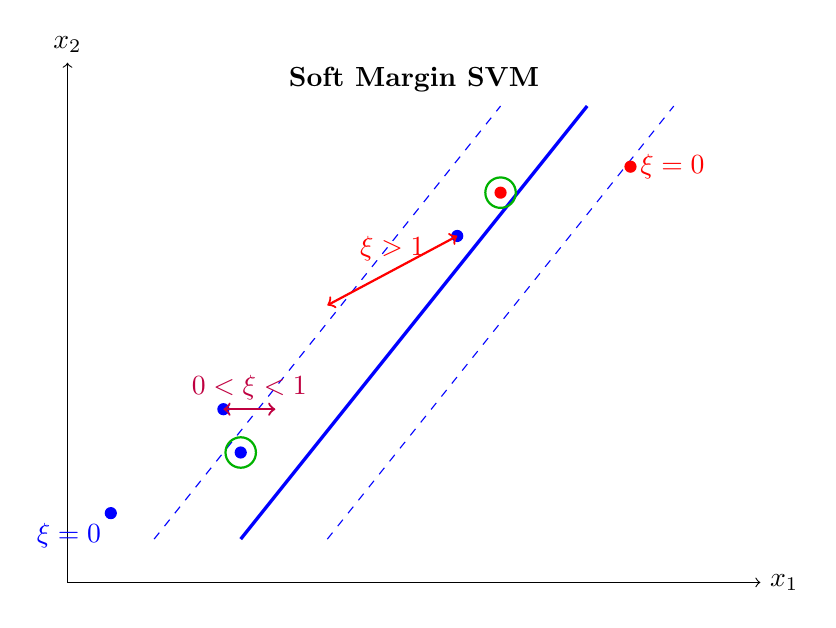
\begin{tikzpicture}[scale=1.1]
    \draw[->] (0,0) -- (8,0) node[right] {$x_1$};
    \draw[->] (0,0) -- (0,6) node[above] {$x_2$};
    
    % Decision boundary
    \draw[very thick, blue] (2,0.5) -- (6,5.5);
    
    % Margin boundaries
    \draw[dashed, blue] (1,0.5) -- (5,5.5);
    \draw[dashed, blue] (3,0.5) -- (7,5.5);
    
    % Good points (outside margin)
    \fill[blue] (0.5,0.8) circle (2pt) node[below left] {$\xi=0$};
    \fill[red] (6.5,4.8) circle (2pt) node[right] {$\xi=0$};
    
    % Point in margin (0 < ξ < 1)
    \fill[blue] (1.8,2) circle (2pt);
    \draw[<->, thick, purple] (1.8,2) -- (2.4,2);
    \node[purple, above] at (2.1,2) {$0 < \xi < 1$};
    
    % Misclassified point (ξ > 1)
    \fill[blue] (4.5,4) circle (2pt);
    \draw[<->, thick, red] (4.5,4) -- (3,3.2);
    \node[red, above] at (3.75,3.6) {$\xi > 1$};
    
    % Support vectors
    \fill[blue] (2,1.5) circle (2pt);
    \draw[green!70!black, thick] (2,1.5) circle (5pt);
    \fill[red] (5,4.5) circle (2pt);
    \draw[green!70!black, thick] (5,4.5) circle (5pt);
    
    \node at (4, 5.8) {\textbf{Soft Margin SVM}};
\end{tikzpicture}
\end{center}

The slack variable $\xi_i$ measures how much point $i$ violates the margin.
\end{geometrybox}

\subsection{Soft Margin Optimization}

\begin{theorem}[Soft Margin SVM (Primal)]
\begin{equation}
    \boxed{
    \begin{aligned}
        \min_{\mathbf{w}, b, \boldsymbol{\xi}} \quad & \frac{1}{2}||\mathbf{w}||^2 + C\sum_{i=1}^{n}\xi_i \\
        \text{subject to} \quad & y_i(\mathbf{w}^T\mathbf{x}_i + b) \geq 1 - \xi_i, \quad i = 1, \ldots, n \\
        & \xi_i \geq 0, \quad i = 1, \ldots, n
    \end{aligned}
    }
\end{equation}

\textbf{Components:}
\begin{itemize}
    \item $\frac{1}{2}||\mathbf{w}||^2$: Maximize margin (model complexity)
    \item $C\sum_{i}\xi_i$: Minimize violations (empirical error)
    \item $C > 0$: Regularization parameter (trade-off)
\end{itemize}
\end{theorem}

\begin{keyidea}
\textbf{The parameter $C$ controls the trade-off:}

\textbf{Large $C$:}
\begin{itemize}
    \item Strong penalty for violations
    \item Tries to classify all points correctly
    \item Smaller margin, more complex boundary
    \item Risk: Overfitting
\end{itemize}

\textbf{Small $C$:}
\begin{itemize}
    \item Weak penalty for violations
    \item Allows more misclassifications
    \item Larger margin, simpler boundary
    \item Risk: Underfitting
\end{itemize}

\textbf{Special cases:}
\begin{itemize}
    \item $C \to \infty$: Hard margin SVM (no violations allowed)
    \item $C \to 0$: Ignore data, just maximize margin
\end{itemize}
\end{keyidea}

\subsection{Soft Margin Dual}

\begin{theorem}[Soft Margin SVM (Dual)]
\begin{equation}
    \boxed{
    \begin{aligned}
        \max_{\boldsymbol{\alpha}} \quad & \sum_{i=1}^{n}\alpha_i - \frac{1}{2}\sum_{i=1}^{n}\sum_{j=1}^{n}\alpha_i\alpha_j y_i y_j \mathbf{x}_i^T\mathbf{x}_j \\
        \text{subject to} \quad & 0 \leq \alpha_i \leq C, \quad i = 1, \ldots, n \\
        & \sum_{i=1}^{n}\alpha_i y_i = 0
    \end{aligned}
    }
\end{equation}

\textbf{Only difference from hard margin:} Box constraint $0 \leq \alpha_i \leq C$ instead of $\alpha_i \geq 0$.
\end{theorem}

\begin{definition}[Support Vectors in Soft Margin]
Points fall into three categories:

\begin{enumerate}
    \item \textbf{$\alpha_i = 0$:} Outside margin (correctly classified)
    \item \textbf{$0 < \alpha_i < C$:} On the margin ($\xi_i = 0$)
    \item \textbf{$\alpha_i = C$:} Violating margin or misclassified ($\xi_i > 0$)
\end{enumerate}

Support vectors are points with $\alpha_i > 0$ (categories 2 and 3).
\end{definition}

\section{The Kernel Trick}

\subsection{Non-Linear Classification}

\begin{mentalmodel}
\textbf{Problem:} What if data is not linearly separable even with slack variables?

\textbf{Example:} XOR problem - two classes arranged in a checkerboard pattern. No straight line can separate them!

\textbf{Idea:} Transform data to a higher-dimensional space where it becomes linearly separable!
\end{mentalmodel}

\begin{geometrybox}
\textbf{The Kernel Trick Concept:}

\begin{center}
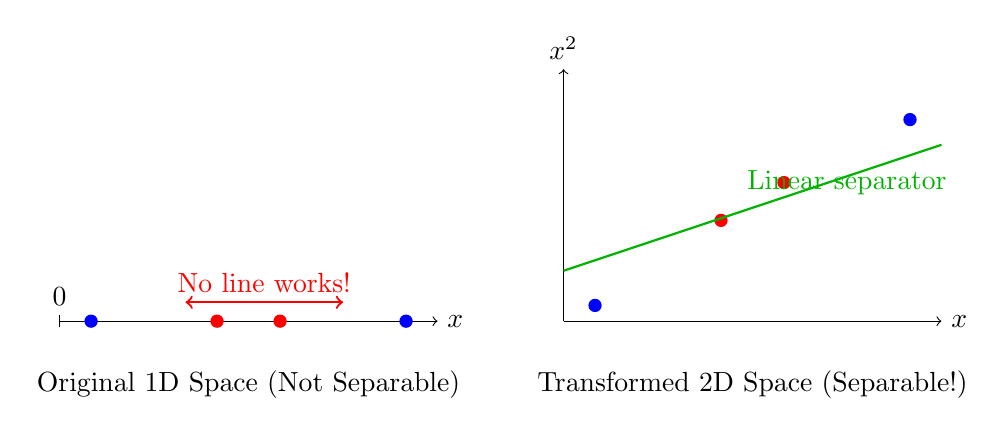
\begin{tikzpicture}[scale=0.8]
    % Original 1D space
    \begin{scope}
        \draw[->] (0,0) -- (6,0) node[right] {$x$};
        \draw (0,-0.1) -- (0,0.1) node[above] {0};
        
        % Class 1 (outside)
        \foreach \x in {0.5, 5.5} {
            \fill[blue] (\x, 0) circle (3pt);
        }
        
        % Class 2 (middle)
        \foreach \x in {2.5, 3.5} {
            \fill[red] (\x, 0) circle (3pt);
        }
        
        \node at (3, -1) {Original 1D Space (Not Separable)};
        \draw[<->, red, thick] (2,0.3) -- (4.5,0.3);
        \node[red] at (3.25, 0.6) {No line works!};
    \end{scope}
    
    % Transformed 2D space
    \begin{scope}[shift={(8,0)}]
        \draw[->] (0,0) -- (6,0) node[right] {$x$};
        \draw[->] (0,0) -- (0,4) node[above] {$x^2$};
        
        % Transformed points
        \fill[blue] (0.5, 0.25) circle (3pt);
        \fill[blue] (5.5, 3.2) circle (3pt);
        \fill[red] (2.5, 1.6) circle (3pt);
        \fill[red] (3.5, 2.2) circle (3pt);
        
        % Separating line
        \draw[thick, green!70!black] (0, 0.8) -- (6, 2.8);
        
        \node at (3, -1) {Transformed 2D Space (Separable!)};
        \node[green!70!black] at (4.5, 2.2) {Linear separator};
    \end{scope}
\end{tikzpicture}
\end{center}

By mapping $x \to [x, x^2]$, we can now separate with a line!
\end{geometrybox}

\subsection{Feature Maps}

\begin{definition}[Feature Map]
A \textbf{feature map} $\phi: \mathbb{R}^p \to \mathbb{R}^d$ (where $d > p$) transforms input to higher dimensions:

\begin{equation}
    \mathbf{x} \mapsto \phi(\mathbf{x})
\end{equation}

\textbf{Example:} For 2D input $\mathbf{x} = [x_1, x_2]^T$:

\begin{equation}
    \phi(\mathbf{x}) = [1, x_1, x_2, x_1^2, x_2^2, x_1 x_2, \ldots]^T
\end{equation}

Apply linear SVM in the transformed space!
\end{definition}

\begin{importantbox}
\textbf{The Problem:}

If $\phi$ maps to very high dimensions (or even infinite dimensions!), computing $\phi(\mathbf{x})$ and $\phi(\mathbf{x})^T\phi(\mathbf{z})$ becomes intractable.

\textbf{The Solution: Kernel Trick}

Notice that SVM dual only needs inner products $\mathbf{x}_i^T\mathbf{x}_j$.

In transformed space, we need $\phi(\mathbf{x}_i)^T\phi(\mathbf{x}_j)$.

\textbf{Key insight:} We can compute $\phi(\mathbf{x}_i)^T\phi(\mathbf{x}_j)$ \textbf{without} explicitly computing $\phi(\mathbf{x})$!
\end{importantbox}

\subsection{Kernel Functions}

\begin{definition}[Kernel Function]
A \textbf{kernel} is a function $K: \mathbb{R}^p \times \mathbb{R}^p \to \mathbb{R}$ such that:

\begin{equation}
    K(\mathbf{x}, \mathbf{z}) = \phi(\mathbf{x})^T\phi(\mathbf{z})
\end{equation}

for some feature map $\phi$.

\textbf{Magic:} We can compute the inner product in high-dimensional space using only the original input!
\end{definition}

\begin{example}[Polynomial Kernel]

\textbf{Feature map:} For $\mathbf{x} = [x_1, x_2]^T$:
\begin{equation}
    \phi(\mathbf{x}) = [1, \sqrt{2}x_1, \sqrt{2}x_2, x_1^2, x_2^2, \sqrt{2}x_1 x_2]^T
\end{equation}

\textbf{Direct computation:}
\begin{align}
    \phi(\mathbf{x})^T\phi(\mathbf{z}) &= 1 + 2x_1 z_1 + 2x_2 z_2 + x_1^2 z_1^2 + x_2^2 z_2^2 + 2x_1 x_2 z_1 z_2
\end{align}

\textbf{Using kernel:}
\begin{equation}
    K(\mathbf{x}, \mathbf{z}) = (1 + \mathbf{x}^T\mathbf{z})^2
\end{equation}

Let's verify:
\begin{align}
    (1 + \mathbf{x}^T\mathbf{z})^2 &= (1 + x_1 z_1 + x_2 z_2)^2 \\
    &= 1 + 2x_1 z_1 + 2x_2 z_2 + x_1^2 z_1^2 + x_2^2 z_2^2 + 2x_1 x_2 z_1 z_2
\end{align}

Same result! But kernel is much simpler to compute.
\end{example}

\subsection{Popular Kernels}

\begin{definition}[Common Kernel Functions]

\textbf{1. Linear Kernel:}
\begin{equation}
    K(\mathbf{x}, \mathbf{z}) = \mathbf{x}^T\mathbf{z}
\end{equation}
(Standard linear SVM)

\textbf{2. Polynomial Kernel:}
\begin{equation}
    K(\mathbf{x}, \mathbf{z}) = (\gamma \mathbf{x}^T\mathbf{z} + r)^d
\end{equation}
where $d$ is the degree, $\gamma > 0$, $r \geq 0$

\textbf{3. Radial Basis Function (RBF) / Gaussian Kernel:}
\begin{equation}
    K(\mathbf{x}, \mathbf{z}) = \exp\left(-\gamma ||\mathbf{x} - \mathbf{z}||^2\right)
\end{equation}
where $\gamma > 0$ controls the width

\textbf{4. Sigmoid Kernel:}
\begin{equation}
    K(\mathbf{x}, \mathbf{z}) = \tanh(\gamma \mathbf{x}^T\mathbf{z} + r)
\end{equation}
\end{definition}

\begin{keyidea}
\textbf{RBF Kernel is the most popular:}

\begin{itemize}
    \item Maps to \textbf{infinite} dimensional space!
    \item $\gamma$ controls complexity:
    \begin{itemize}
        \item Small $\gamma$: smooth decision boundary (underfitting risk)
        \item Large $\gamma$: wiggly decision boundary (overfitting risk)
    \end{itemize}
    \item Works well for many problems
    \item Default choice for many applications
\end{itemize}
\end{keyidea}

\subsection{Kernelized SVM}

\begin{theorem}[SVM with Kernels]
Replace all inner products $\mathbf{x}_i^T\mathbf{x}_j$ with $K(\mathbf{x}_i, \mathbf{x}_j)$:

\textbf{Dual:}
\begin{equation}
    \max_{\boldsymbol{\alpha}} \sum_{i=1}^{n}\alpha_i - \frac{1}{2}\sum_{i=1}^{n}\sum_{j=1}^{n}\alpha_i\alpha_j y_i y_j K(\mathbf{x}_i, \mathbf{x}_j)
\end{equation}

\textbf{Decision function:}
\begin{equation}
    f(\mathbf{x}_{\text{new}}) = \sum_{i \in SV}\alpha_i y_i K(\mathbf{x}_i, \mathbf{x}_{\text{new}}) + b
\end{equation}

\textbf{We never explicitly compute $\phi(\mathbf{x})$!}
\end{theorem}

\section{Multi-Class SVM}

\begin{definition}[Multi-Class Strategies]
SVM is inherently binary. For $K > 2$ classes:

\textbf{1. One-vs-Rest (OvR):}
\begin{itemize}
    \item Train $K$ binary classifiers
    \item Classifier $k$: Class $k$ vs all others
    \item Predict: Class with highest decision function value
\end{itemize}

\textbf{2. One-vs-One (OvO):}
\begin{itemize}
    \item Train $\binom{K}{2} = \frac{K(K-1)}{2}$ binary classifiers
    \item One classifier for each pair of classes
    \item Predict: Majority voting among all classifiers
\end{itemize}

\textbf{OvO is generally preferred:} Each classifier trains on less data (only 2 classes), more accurate.
\end{definition}

\section{Computational Complexity}

\begin{definition}[SVM Complexity]

\textbf{Training:}
\begin{itemize}
    \item Quadratic programming: $O(n^2 p)$ to $O(n^3)$
    \item With specialized algorithms (SMO): $O(n^2)$ to $O(n^{2.3})$
    \item Slow for very large $n$ (>100,000)
\end{itemize}

\textbf{Prediction:}
\begin{itemize}
    \item $O(nsv \cdot p)$ where $nsv$ is number of support vectors
    \item Typically $nsv << n$, so quite fast
\end{itemize}

\textbf{Space:}
\begin{itemize}
    \item Must store support vectors
    \item $O(nsv \cdot p)$
\end{itemize}
\end{definition}

\section{Advantages and Disadvantages}

\begin{keyidea}
\textbf{Advantages:}

\begin{enumerate}
    \item \textbf{Effective in high dimensions:} Works well when $p >> n$
    \item \textbf{Memory efficient:} Only stores support vectors
    \item \textbf{Versatile:} Different kernels for different problems
    \item \textbf{Robust:} Maximum margin → good generalization
    \item \textbf{Convex optimization:} Global optimum guaranteed
    \item \textbf{Works with small datasets:} Doesn't need massive data
    \item \textbf{Handles outliers:} Soft margin allows violations
\end{enumerate}

\textbf{Disadvantages:}

\begin{enumerate}
    \item \textbf{Slow training:} $O(n^2)$ or worse for large $n$
    \item \textbf{No probability estimates:} (without additional calibration)
    \item \textbf{Parameter tuning:} Need to choose $C$, kernel, kernel parameters
    \item \textbf{Not interpretable:} Hard to understand decision (unlike decision trees)
    \item \textbf{Sensitive to feature scaling:} Must normalize features
    \item \textbf{Memory for kernels:} Must store kernel matrix or support vectors
    \item \textbf{Multi-class is indirect:} Not naturally multi-class
\end{enumerate}
\end{keyidea}

\section{GATE-Style Problems}

\begin{example}[Problem 1: Margin Calculation]

\textbf{Given:} Hyperplane $3x_1 + 4x_2 - 10 = 0$ in canonical form.

\textbf{Find:} The margin width.

\textbf{Solution:}

From $\mathbf{w}^T\mathbf{x} + b = 0$: $\mathbf{w} = [3, 4]^T$

\begin{align}
    ||\mathbf{w}|| &= \sqrt{3^2 + 4^2} = \sqrt{25} = 5
\end{align}

\textbf{Margin width:}
\begin{equation}
    \text{width} = \frac{2}{||\mathbf{w}||} = \frac{2}{5} = 0.4
\end{equation}
\end{example}

\begin{example}[Problem 2: Support Vectors]

\textbf{Question:} After training SVM, we get:
\begin{center}
\begin{tabular}{|c|c|c|}
\hline
Point & $\alpha_i$ & $y_i(\mathbf{w}^T\mathbf{x}_i + b)$ \\
\hline
1 & 0 & 2.5 \\
2 & 0.3 & 1.0 \\
3 & 0 & 1.8 \\
4 & 0.5 & 1.0 \\
\hline
\end{tabular}
\end{center}

Which points are support vectors?

\textbf{Solution:}

Support vectors have $\alpha_i > 0$: \textbf{Points 2 and 4}

Also note they lie exactly on the margin ($y_i(\mathbf{w}^T\mathbf{x}_i + b) = 1$).
\end{example}

\begin{example}[Problem 3: Effect of $C$]

\textbf{Question:} What happens to the SVM solution as $C$ increases from 0.01 to 1000?

\textbf{Answer:}

\textbf{As $C$ increases:}
\begin{itemize}
    \item Penalty for violations increases
    \item Fewer points allowed inside margin
    \item Margin becomes smaller
    \item Decision boundary becomes more complex
    \item Risk of overfitting increases
\end{itemize}

\textbf{At $C \to \infty$:} Approaches hard margin SVM (no violations)

\textbf{At $C \to 0$:} Ignores data, maximizes margin regardless of errors
\end{example}

\begin{example}[Problem 4: Kernel Computation]

\textbf{Given:} $\mathbf{x} = [1, 2]^T$, $\mathbf{z} = [3, -1]^T$

\textbf{Compute:} 
\begin{enumerate}
    \item Linear kernel: $K(\mathbf{x}, \mathbf{z})$
    \item Polynomial kernel (degree 2): $K(\mathbf{x}, \mathbf{z}) = (\mathbf{x}^T\mathbf{z} + 1)^2$
    \item RBF kernel: $K(\mathbf{x}, \mathbf{z}) = \exp(-0.5||\mathbf{x} - \mathbf{z}||^2)$
\end{enumerate}

\textbf{Solution:}

\textbf{Linear:}
\begin{equation}
    K(\mathbf{x}, \mathbf{z}) = 1(3) + 2(-1) = 3 - 2 = 1
\end{equation}

\textbf{Polynomial:}
\begin{equation}
    K(\mathbf{x}, \mathbf{z}) = (1 + 1)^2 = 4
\end{equation}

\textbf{RBF:}
\begin{align}
    ||\mathbf{x} - \mathbf{z}||^2 &= (1-3)^2 + (2-(-1))^2 = 4 + 9 = 13 \\
    K(\mathbf{x}, \mathbf{z}) &= \exp(-0.5 \times 13) = \exp(-6.5) \approx 0.0015
\end{align}
\end{example}

\section{Summary - Key Points for GATE}

\begin{importantbox}
\textbf{Must Know for GATE:}

\begin{enumerate}
    \item \textbf{Maximum margin principle:} Choose hyperplane farthest from both classes
    
    \item \textbf{Margin width:} $\frac{2}{||\mathbf{w}||}$ in canonical form
    
    \item \textbf{Hard margin SVM:}
    \begin{equation}
        \min \frac{1}{2}||\mathbf{w}||^2 \quad \text{s.t.} \quad y_i(\mathbf{w}^T\mathbf{x}_i + b) \geq 1
    \end{equation}
    
    \item \textbf{Soft margin SVM:}
    \begin{equation}
        \min \frac{1}{2}||\mathbf{w}||^2 + C\sum_i \xi_i \quad \text{s.t.} \quad y_i(\mathbf{w}^T\mathbf{x}_i + b) \geq 1 - \xi_i
    \end{equation}
    
    \item \textbf{Support vectors:} Points with $\alpha_i > 0$ (on or inside margin)
    
    \item \textbf{Decision function:}
    \begin{equation}
        f(\mathbf{x}) = \sum_{i \in SV} \alpha_i y_i K(\mathbf{x}_i, \mathbf{x}) + b
    \end{equation}
    
    \item \textbf{Parameter $C$:}
    \begin{itemize}
        \item Large $C$: Small margin, few violations (overfitting risk)
        \item Small $C$: Large margin, more violations (underfitting risk)
    \end{itemize}
    
    \item \textbf{Kernels:}
    \begin{itemize}
        \item Linear: $\mathbf{x}^T\mathbf{z}$
        \item Polynomial: $(\gamma \mathbf{x}^T\mathbf{z} + r)^d$
        \item RBF: $\exp(-\gamma||\mathbf{x} - \mathbf{z}||^2)$
    \end{itemize}
    
    \item \textbf{Kernel trick:} Compute $\phi(\mathbf{x})^T\phi(\mathbf{z})$ without computing $\phi$
    
    \item \textbf{Multi-class:} One-vs-Rest or One-vs-One
    
    \item \textbf{Complexity:} Training $O(n^2)$ to $O(n^3)$, Prediction $O(nsv \cdot p)$
    
    \item \textbf{Key properties:}
    \begin{itemize}
        \item Convex optimization (global optimum)
        \item Sparse solution (only support vectors matter)
        \item Works in high dimensions
        \item Effective with small datasets
    \end{itemize}
\end{enumerate}
\end{importantbox}

\begin{gatepoint}
\textbf{Common GATE Question Types:}

\begin{enumerate}
    \item Calculate margin width from $\mathbf{w}$
    \item Identify support vectors from $\alpha_i$ values
    \item Understand effect of $C$ on solution
    \item Compute kernel function values
    \item Explain kernel trick concept
    \item Compare hard vs soft margin
    \item Understand slack variables $\xi_i$
    \item Know when to use which kernel
    \item Explain maximum margin principle
    \item Compare SVM with other classifiers (LDA, logistic regression)
    \item Understand dual formulation
    \item Know multi-class strategies
\end{enumerate}
\end{gatepoint}
\chapter{Decision Trees: Intuitive Tree-Based Classification and Regression}

\section{Introduction to Decision Trees}

\begin{mentalmodel}
Imagine you're a doctor diagnosing a patient. You might think:

\textbf{Question 1:} "Does the patient have a fever?"
\begin{itemize}
    \item If YES → Ask: "Does the patient have a cough?"
    \begin{itemize}
        \item If YES → Diagnose: Flu
        \item If NO → Diagnose: Infection
    \end{itemize}
    \item If NO → Ask: "Does the patient have a rash?"
    \begin{itemize}
        \item If YES → Diagnose: Allergy
        \item If NO → Diagnose: Healthy
    \end{itemize}
\end{itemize}

\textbf{This is exactly how a decision tree works!}

A series of yes/no questions leading to a decision.
\end{mentalmodel}

\begin{keyidea}
Decision Trees are a \textbf{non-parametric} supervised learning method used for both classification and regression.

\textbf{Core idea:} Recursively split the data based on feature values to create a tree structure where:
\begin{itemize}
    \item \textbf{Internal nodes:} Represent decisions/tests on features
    \item \textbf{Branches:} Represent outcomes of tests
    \item \textbf{Leaf nodes:} Represent final predictions (class labels or values)
\end{itemize}

\textbf{Key advantages:}
\begin{itemize}
    \item Highly interpretable (can be visualized and explained)
    \item No feature scaling needed
    \item Handles both numerical and categorical data
    \item Captures non-linear relationships
\end{itemize}
\end{keyidea}

\section{Tree Structure and Terminology}

\begin{definition}[Decision Tree Components]

\textbf{1. Root Node:} The topmost node representing the entire dataset

\textbf{2. Internal/Decision Nodes:} Nodes that split the data based on a feature test

\textbf{3. Leaf/Terminal Nodes:} Nodes that make final predictions (no further splits)

\textbf{4. Branch/Edge:} Connection between nodes representing test outcomes

\textbf{5. Parent/Child:} Node that splits is parent; resulting nodes are children

\textbf{6. Depth:} Length of longest path from root to leaf

\textbf{7. Split:} Division of data at a node based on feature test
\end{definition}

\begin{geometrybox}
\textbf{Example Decision Tree Structure:}

\begin{center}
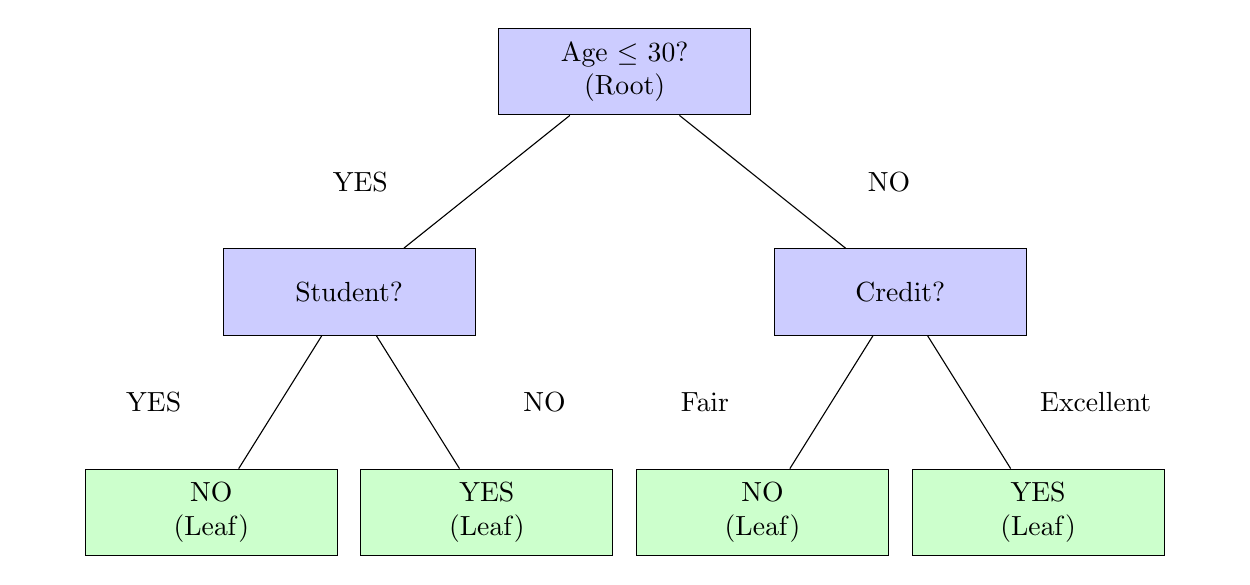
\begin{tikzpicture}[
    level distance=2.8cm,                % more vertical space
    level 1/.style={sibling distance=7cm},
    level 2/.style={sibling distance=3.5cm},
    every node/.style={
        draw,
        rectangle,
        minimum width=3.2cm,             % wider nodes
        minimum height=1.1cm,
        align=center
    },
    leaf/.style={fill=green!20},
    decision/.style={fill=blue!20}
]

\node[decision] {Age $\leq$ 30?\\(Root)}
    child {
        node[decision] {Student?}
        child {
            node[leaf] {NO\\(Leaf)}
            edge from parent node[left, draw=none] {YES}
        }
        child {
            node[leaf] {YES\\(Leaf)}
            edge from parent node[right, draw=none] {NO}
        }
        edge from parent node[left, draw=none] {YES}
    }
    child {
        node[decision] {Credit?}
        child {
            node[leaf] {NO\\(Leaf)}
            edge from parent node[left, draw=none] {Fair}
        }
        child {
            node[leaf] {YES\\(Leaf)}
            edge from parent node[right, draw=none] {Excellent}
        }
        edge from parent node[right, draw=none] {NO}
    };

\end{tikzpicture}
\end{center}

\textbf{Reading the tree:}
\begin{itemize}
    \item Start at root: "Is Age $\leq$ 30?"
    \item If YES, go left: "Is Student?"
    \item If Student is YES → Predict NO
    \item If Student is NO → Predict YES
\end{itemize}

This tree predicts whether someone will buy a product based on Age, Student status, and Credit rating.
\end{geometrybox}

\section{Building a Decision Tree: The Algorithm}

\subsection{Basic Recursive Algorithm}

\begin{definition}[Tree Construction Algorithm]

\textbf{Function:} BuildTree(Data, Features)

\textbf{Base Cases (Stop Splitting):}
\begin{enumerate}
    \item All samples belong to same class → Create leaf with that class
    \item No features left to split on → Create leaf with majority class
    \item Maximum depth reached → Create leaf with majority class
    \item Number of samples below minimum threshold → Create leaf
\end{enumerate}

\textbf{Recursive Case:}
\begin{enumerate}
    \item Select best feature to split on (using splitting criterion)
    \item Create decision node for this feature
    \item Partition data based on feature values
    \item For each partition:
    \begin{itemize}
        \item Recursively call BuildTree on subset
        \item Create child node
    \end{itemize}
    \item Return the tree
\end{enumerate}
\end{definition}

\begin{mentalmodel}
\textbf{The key question:} How do we choose the "best" feature to split on?

We need a measure of "how good" a split is. This is where \textbf{splitting criteria} come in!

Good split: Separates classes well (creates "pure" subsets)

Bad split: Mixes classes (creates "impure" subsets)
\end{mentalmodel}

\section{Splitting Criteria for Classification}

\subsection{Entropy and Information Gain}

\begin{definition}[Entropy]
\textbf{Entropy} measures the impurity/disorder in a set of samples.

For a dataset $S$ with $K$ classes:
\begin{equation}
    H(S) = -\sum_{k=1}^{K} p_k \log_2 p_k
\end{equation}

where $p_k$ is the proportion of samples in class $k$.

\textbf{Properties:}
\begin{itemize}
    \item $H(S) = 0$: Pure (all samples same class) - \textbf{Perfect!}
    \item $H(S) = \log_2 K$: Maximum impurity (uniform distribution) - \textbf{Worst!}
    \item $0 \leq H(S) \leq \log_2 K$
\end{itemize}
\end{definition}

\begin{example}[Computing Entropy]

\textbf{Dataset 1:} 10 samples, all Class A
\begin{align}
    p_A &= \frac{10}{10} = 1.0 \\
    H(S) &= -(1.0 \log_2 1.0) = -(1.0 \times 0) = 0
\end{align}

\textbf{Perfect purity!} No uncertainty.

\textbf{Dataset 2:} 10 samples, 5 Class A, 5 Class B
\begin{align}
    p_A &= 0.5, \quad p_B = 0.5 \\
    H(S) &= -(0.5 \log_2 0.5 + 0.5 \log_2 0.5) \\
    &= -(0.5 \times (-1) + 0.5 \times (-1)) \\
    &= -(-0.5 - 0.5) = 1.0
\end{align}

\textbf{Maximum impurity!} (for 2 classes)

\textbf{Dataset 3:} 10 samples, 8 Class A, 2 Class B
\begin{align}
    p_A &= 0.8, \quad p_B = 0.2 \\
    H(S) &= -(0.8 \log_2 0.8 + 0.2 \log_2 0.2) \\
    &= -(0.8 \times (-0.322) + 0.2 \times (-2.322)) \\
    &= -(-0.258 - 0.464) = 0.722
\end{align}

\textbf{Some impurity,} but better than Dataset 2.
\end{example}

\begin{definition}[Information Gain]
\textbf{Information Gain (IG)} measures how much entropy is reduced by splitting on a feature.

If we split dataset $S$ using feature $A$ into subsets $\{S_1, S_2, \ldots, S_v\}$:

\begin{equation}
    IG(S, A) = H(S) - \sum_{i=1}^{v} \frac{|S_i|}{|S|} H(S_i)
\end{equation}

\textbf{Components:}
\begin{itemize}
    \item $H(S)$: Entropy before split
    \item $\sum_{i} \frac{|S_i|}{|S|} H(S_i)$: Weighted average entropy after split
    \item Higher IG → Better split!
\end{itemize}

\textbf{Decision rule:} Choose feature with \textbf{maximum Information Gain}.
\end{definition}

\begin{example}[Information Gain Calculation]

\textbf{Dataset:} 14 samples for "Play Tennis?"

\begin{center}
\begin{tabular}{|c|c|}
\hline
Outcome & Count \\
\hline
Yes & 9 \\
No & 5 \\
\hline
Total & 14 \\
\hline
\end{tabular}
\end{center}

\textbf{STEP 1: Calculate entropy of dataset}
\begin{align}
    p_{Yes} &= \frac{9}{14} \approx 0.643, \quad p_{No} = \frac{5}{14} \approx 0.357 \\
    H(S) &= -(0.643 \log_2 0.643 + 0.357 \log_2 0.357) \\
    &= -(0.643 \times (-0.637) + 0.357 \times (-1.486)) \\
    &= -(-0.410 - 0.531) = 0.941
\end{align}

\textbf{STEP 2: Consider splitting on "Outlook" (Sunny, Overcast, Rainy)}

\begin{center}
\begin{tabular}{|c|c|c|c|}
\hline
Outlook & Yes & No & Total \\
\hline
Sunny & 2 & 3 & 5 \\
Overcast & 4 & 0 & 4 \\
Rainy & 3 & 2 & 5 \\
\hline
\end{tabular}
\end{center}

\textbf{Entropy for Sunny:}
\begin{align}
    p_{Yes} &= \frac{2}{5} = 0.4, \quad p_{No} = \frac{3}{5} = 0.6 \\
    H(\text{Sunny}) &= -(0.4 \log_2 0.4 + 0.6 \log_2 0.6) \\
    &= -(0.4 \times (-1.322) + 0.6 \times (-0.737)) \\
    &= 0.971
\end{align}

\textbf{Entropy for Overcast:}
\begin{align}
    p_{Yes} &= \frac{4}{4} = 1.0, \quad p_{No} = 0 \\
    H(\text{Overcast}) &= -(1.0 \log_2 1.0) = 0
\end{align}

\textbf{Entropy for Rainy:}
\begin{align}
    p_{Yes} &= \frac{3}{5} = 0.6, \quad p_{No} = \frac{2}{5} = 0.4 \\
    H(\text{Rainy}) &= -(0.6 \log_2 0.6 + 0.4 \log_2 0.4) \\
    &= 0.971
\end{align}

\textbf{Weighted average entropy after split:}
\begin{align}
    H_{\text{after}} &= \frac{5}{14}(0.971) + \frac{4}{14}(0) + \frac{5}{14}(0.971) \\
    &= 0.347 + 0 + 0.347 = 0.694
\end{align}

\textbf{Information Gain:}
\begin{equation}
    IG(S, \text{Outlook}) = 0.941 - 0.694 = 0.247
\end{equation}

\textbf{Interpretation:} Splitting on Outlook reduces entropy by 0.247 bits!

We would calculate IG for all features and choose the one with highest IG.
\end{example}

\subsection{Gini Impurity}

\begin{definition}[Gini Index]
The \textbf{Gini Impurity} (or Gini Index) is another measure of impurity:

\begin{equation}
    \text{Gini}(S) = 1 - \sum_{k=1}^{K} p_k^2
\end{equation}

\textbf{Properties:}
\begin{itemize}
    \item $\text{Gini}(S) = 0$: Pure (all same class)
    \item $\text{Gini}(S) = 1 - \frac{1}{K}$: Maximum impurity (uniform distribution)
    \item $0 \leq \text{Gini}(S) < 1$
\end{itemize}

\textbf{Gini Gain:}
\begin{equation}
    \text{Gini Gain}(S, A) = \text{Gini}(S) - \sum_{i=1}^{v} \frac{|S_i|}{|S|} \text{Gini}(S_i)
\end{equation}
\end{definition}

\begin{example}[Gini vs Entropy]

\textbf{Dataset:} 10 samples, 5 Class A, 5 Class B

\textbf{Entropy:}
\begin{equation}
    H(S) = -(0.5 \log_2 0.5 + 0.5 \log_2 0.5) = 1.0
\end{equation}

\textbf{Gini:}
\begin{equation}
    \text{Gini}(S) = 1 - (0.5^2 + 0.5^2) = 1 - 0.5 = 0.5
\end{equation}

Different scales, but both indicate maximum impurity for 2 classes.
\end{example}

\begin{importantbox}
\textbf{Entropy vs Gini: Which to use?}

\textbf{Entropy (Information Gain):}
\begin{itemize}
    \item Used in ID3, C4.5 algorithms
    \item Theoretically grounded in information theory
    \item Computationally more expensive (logarithm)
    \item Slightly more sensitive to class distribution
\end{itemize}

\textbf{Gini Impurity:}
\begin{itemize}
    \item Used in CART algorithm
    \item Computationally faster (no logarithm)
    \item Often gives similar trees to entropy
    \item Preferred in practice (especially in scikit-learn)
\end{itemize}

\textbf{In practice:} They usually give very similar results. Gini is faster, so it's often preferred.
\end{importantbox}

\subsection{Classification Error}

\begin{definition}[Classification Error]
Another (less commonly used) splitting criterion:

\begin{equation}
    \text{Error}(S) = 1 - \max_k p_k
\end{equation}

This is simply the probability of misclassification if we predict the majority class.

\textbf{Problem:} Less sensitive to changes in class distribution, so rarely used in practice.
\end{definition}

\section{Splitting Criteria for Regression}

\begin{definition}[Variance Reduction]
For regression trees, we use \textbf{variance} instead of entropy/Gini.

\textbf{Variance of target values in set $S$:}
\begin{equation}
    \text{Var}(S) = \frac{1}{|S|}\sum_{i \in S}(y_i - \bar{y})^2
\end{equation}

where $\bar{y} = \frac{1}{|S|}\sum_{i \in S} y_i$ is the mean.

\textbf{Variance Reduction (analogous to Information Gain):}
\begin{equation}
    VR(S, A) = \text{Var}(S) - \sum_{i=1}^{v} \frac{|S_i|}{|S|} \text{Var}(S_i)
\end{equation}

Choose split that \textbf{maximizes variance reduction}.
\end{definition}

\begin{example}[Regression Tree Split]

\textbf{Dataset:} House prices (in \$1000s)

\begin{center}
\begin{tabular}{|c|c|}
\hline
Size (sq ft) & Price \\
\hline
1000 & 200 \\
1500 & 250 \\
2000 & 300 \\
2500 & 350 \\
3000 & 400 \\
\hline
\end{tabular}
\end{center}

\textbf{Consider split: Size $\leq$ 2000}

\textbf{Left subset (Size $\leq$ 2000):} \{200, 250, 300\}
\begin{align}
    \bar{y}_L &= \frac{200 + 250 + 300}{3} = 250 \\
    \text{Var}(S_L) &= \frac{(200-250)^2 + (250-250)^2 + (300-250)^2}{3} \\
    &= \frac{2500 + 0 + 2500}{3} = \frac{5000}{3} \approx 1667
\end{align}

\textbf{Right subset (Size $>$ 2000):} \{350, 400\}
\begin{align}
    \bar{y}_R &= \frac{350 + 400}{2} = 375 \\
    \text{Var}(S_R) &= \frac{(350-375)^2 + (400-375)^2}{2} \\
    &= \frac{625 + 625}{2} = 625
\end{align}

\textbf{Original variance:}
\begin{align}
    \bar{y} &= \frac{200 + 250 + 300 + 350 + 400}{5} = 300 \\
    \text{Var}(S) &= \frac{(200-300)^2 + \cdots + (400-300)^2}{5} \\
    &= \frac{10000 + 2500 + 0 + 2500 + 10000}{5} = 5000
\end{align}

\textbf{Variance Reduction:}
\begin{align}
    VR &= 5000 - \left(\frac{3}{5} \times 1667 + \frac{2}{5} \times 625\right) \\
    &= 5000 - (1000 + 250) = 5000 - 1250 = 3750
\end{align}

This split reduces variance by 3750!
\end{example}

\section{Handling Different Feature Types}

\subsection{Categorical Features}

\begin{definition}[Splitting on Categorical Features]
\smallskip
\textbf{Binary feature:} Direct split (e.g., Gender: Male/Female)

\textbf{Multi-valued feature:} Multiple approaches

\textbf{Approach 1: Multi-way split}
\begin{itemize}
    \item Create one branch for each value
    \item Example: Color $\in$ \{Red, Green, Blue\} → 3 branches
    \item Problem: Can create many small subsets
\end{itemize}

\textbf{Approach 2: Binary split}
\begin{itemize}
    \item Group values into two subsets
    \item Example: Color $\in$ \{Red, Green\} vs Color $\in$ \{Blue\}
    \item For $k$ values: $2^{k-1} - 1$ possible splits (exponential!)
\end{itemize}

\textbf{In practice:} Multi-way splits are simpler, binary splits can be more powerful.
\end{definition}

\subsection{Numerical Features}

\begin{definition}[Splitting on Numerical Features]

For a continuous feature, we need to find a \textbf{threshold value} $t$.

\textbf{Split:} $X \leq t$ vs $X > t$

\textbf{Algorithm to find best threshold:}
\begin{enumerate}
    \item Sort all unique values of the feature: $v_1 < v_2 < \cdots < v_m$
    \item Consider midpoints as candidates: $t_i = \frac{v_i + v_{i+1}}{2}$
    \item For each candidate $t_i$:
    \begin{itemize}
        \item Split data: $S_L = \{x : x \leq t_i\}$, $S_R = \{x : x > t_i\}$
        \item Calculate Information Gain or Gini Gain
    \end{itemize}
    \item Choose threshold with maximum gain
\end{enumerate}

\textbf{Complexity:} $O(m \log m)$ for sorting + $O(m \cdot n)$ for evaluating splits
\end{definition}

\begin{example}[Finding Best Threshold]

\textbf{Data:} Ages and class labels

\begin{center}
\begin{tabular}{|c|c|}
\hline
Age & Class \\
\hline
25 & A \\
30 & A \\
35 & B \\
40 & B \\
45 & B \\
\hline
\end{tabular}
\end{center}

\textbf{Candidate thresholds:}
\begin{itemize}
    \item $t_1 = 27.5$ (between 25 and 30)
    \item $t_2 = 32.5$ (between 30 and 35)
    \item $t_3 = 37.5$ (between 35 and 40)
    \item $t_4 = 42.5$ (between 40 and 45)
\end{itemize}

\textbf{Evaluate $t_2 = 32.5$:}
\begin{itemize}
    \item Left: Ages $\leq$ 32.5 → \{25, 30\} → Classes: A, A (pure!)
    \item Right: Ages $>$ 32.5 → \{35, 40, 45\} → Classes: B, B, B (pure!)
\end{itemize}

This split gives \textbf{perfect separation}! IG would be maximum here.
\end{example}

\section{Complete Example: Building a Decision Tree}

\begin{example}[Step-by-Step Tree Construction]

\textbf{Dataset:} Loan Approval (14 samples)

\begin{center}
\begin{tabular}{|c|c|c|c|c|}
\hline
ID & Age & Income & Student & Approved \\
\hline
1 & Youth & High & No & No \\
2 & Youth & High & No & No \\
3 & Middle & High & No & Yes \\
4 & Senior & Medium & No & Yes \\
5 & Senior & Low & Yes & Yes \\
6 & Senior & Low & Yes & No \\
7 & Middle & Low & Yes & Yes \\
8 & Youth & Medium & No & No \\
9 & Youth & Low & Yes & Yes \\
10 & Senior & Medium & Yes & Yes \\
11 & Youth & Medium & Yes & Yes \\
12 & Middle & Medium & No & Yes \\
13 & Middle & High & Yes & Yes \\
14 & Senior & Medium & No & No \\
\hline
\end{tabular}
\end{center}

\textbf{Class distribution:} 9 Yes, 5 No

\textbf{STEP 1: Calculate root entropy}
\begin{align}
    H(S) &= -\left(\frac{9}{14}\log_2\frac{9}{14} + \frac{5}{14}\log_2\frac{5}{14}\right) \\
    &= -(0.643 \times (-0.637) + 0.357 \times (-1.486)) \\
    &\approx 0.940
\end{align}

\textbf{STEP 2: Calculate IG for each feature}

\textbf{Feature: Age}

\begin{center}
\begin{tabular}{|c|c|c|c|}
\hline
Age & Yes & No & Total \\
\hline
Youth & 2 & 3 & 5 \\
Middle & 4 & 0 & 4 \\
Senior & 3 & 2 & 5 \\
\hline
\end{tabular}
\end{center}

\begin{align}
    H(\text{Youth}) &= -\left(\frac{2}{5}\log_2\frac{2}{5} + \frac{3}{5}\log_2\frac{3}{5}\right) \approx 0.971 \\
    H(\text{Middle}) &= 0 \text{ (all Yes)} \\
    H(\text{Senior}) &= -\left(\frac{3}{5}\log_2\frac{3}{5} + \frac{2}{5}\log_2\frac{2}{5}\right) \approx 0.971
\end{align}

\begin{align}
    IG(\text{Age}) &= 0.940 - \left(\frac{5}{14}(0.971) + \frac{4}{14}(0) + \frac{5}{14}(0.971)\right) \\
    &= 0.940 - 0.694 = 0.246
\end{align}

\textbf{Feature: Income}

\begin{center}
\begin{tabular}{|c|c|c|c|}
\hline
Income & Yes & No & Total \\
\hline
High & 2 & 2 & 4 \\
Medium & 4 & 2 & 6 \\
Low & 3 & 1 & 4 \\
\hline
\end{tabular}
\end{center}

\begin{align}
    H(\text{High}) &= 1.0 \\
    H(\text{Medium}) &\approx 0.918 \\
    H(\text{Low}) &\approx 0.811
\end{align}

\begin{align}
    IG(\text{Income}) &= 0.940 - \left(\frac{4}{14}(1.0) + \frac{6}{14}(0.918) + \frac{4}{14}(0.811)\right) \\
    &= 0.940 - 0.911 = 0.029
\end{align}

\textbf{Feature: Student}

\begin{center}
\begin{tabular}{|c|c|c|c|}
\hline
Student & Yes & No & Total \\
\hline
Yes & 6 & 1 & 7 \\
No & 3 & 4 & 7 \\
\hline
\end{tabular}
\end{center}

\begin{align}
    H(\text{Student=Yes}) &= -\left(\frac{6}{7}\log_2\frac{6}{7} + \frac{1}{7}\log_2\frac{1}{7}\right) \approx 0.592 \\
    H(\text{Student=No}) &= -\left(\frac{3}{7}\log_2\frac{3}{7} + \frac{4}{7}\log_2\frac{4}{7}\right) \approx 0.985
\end{align}

\begin{align}
    IG(\text{Student}) &= 0.940 - \left(\frac{7}{14}(0.592) + \frac{7}{14}(0.985)\right) \\
    &= 0.940 - 0.789 = 0.151
\end{align}

\textbf{STEP 3: Choose best feature}

Information Gains:
\begin{itemize}
    \item Age: 0.246 ← \textbf{Highest!}
    \item Income: 0.029
    \item Student: 0.151
\end{itemize}

\textbf{Split on Age at root!}

\textbf{STEP 4: Create branches and recurse}

\textbf{Branch 1: Age = Middle}
\begin{itemize}
    \item All 4 samples are "Yes" → Create leaf: \textbf{Approved = YES}
\end{itemize}

\textbf{Branch 2: Age = Youth} (5 samples: 2 Yes, 3 No)
\begin{itemize}
    \item Recurse: Calculate IG for Income and Student on this subset
    \item (Exercise: Continue the tree...)
\end{itemize}

\textbf{Branch 3: Age = Senior} (5 samples: 3 Yes, 2 No)
\begin{itemize}
    \item Recurse: Calculate IG for Income and Student on this subset
\end{itemize}

\textbf{Final Tree (simplified):}

\begin{center}
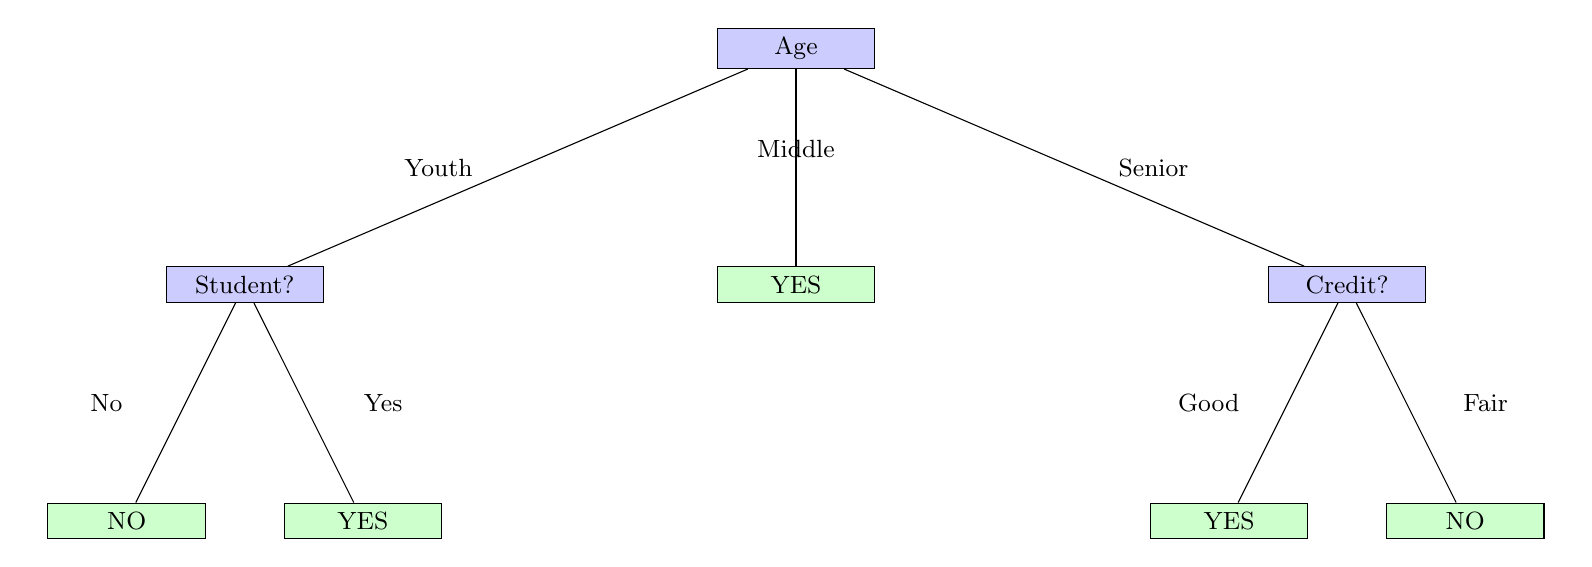
\begin{tikzpicture}[
    level distance=3cm,
    level 1/.style={sibling distance=7cm},
    level 2/.style={sibling distance=3cm},
    every node/.style={draw, rectangle, minimum width=2cm, align=center, font=\small},
    leaf/.style={draw, rectangle, fill=green!20},
    decision/.style={draw, rectangle, fill=blue!20}
]
\node[decision] {Age}
    child {
        node[decision] {Student?}
        child {node[leaf] {NO} edge from parent node[left, draw=none] {No}}
        child {node[leaf] {YES} edge from parent node[right, draw=none] {Yes}}
        edge from parent node[left, draw=none] {Youth}
    }
    child {
        node[leaf] {YES}
        edge from parent node[above, draw=none] {Middle}
    }
    child {
        node[decision] {Credit?}
        child {node[leaf] {YES} edge from parent node[left, draw=none] {Good}}
        child {node[leaf] {NO} edge from parent node[right, draw=none] {Fair}}
        edge from parent node[right, draw=none] {Senior}
    };
\end{tikzpicture}
\end{center}

\end{example}

\section{Overfitting and Pruning}

\subsection{The Overfitting Problem}

\begin{mentalmodel}
\textbf{Unpruned trees can grow very deep:}

If we keep splitting until every leaf is pure:
\begin{itemize}
    \item Tree becomes very complex
    \item Memorizes training data (including noise)
    \item Poor generalization to new data
\end{itemize}

\textbf{Analogy:} Like memorizing the answers to practice problems instead of understanding concepts - you fail on the real exam!
\end{mentalmodel}

\begin{geometrybox}
\textbf{Overfitting Illustration:}

\begin{center}
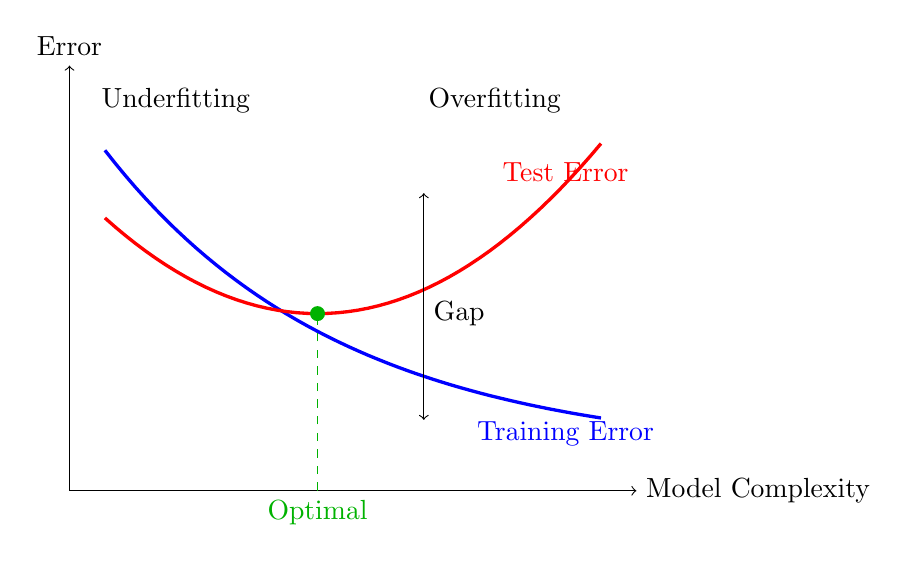
\begin{tikzpicture}[scale=0.9]
    % Axes
    \draw[->] (0,0) -- (8,0) node[right] {Model Complexity};
    \draw[->] (0,0) -- (0,6) node[above] {Error};
    
    % Training error (decreasing)
    \draw[blue, very thick, domain=0.5:7.5, samples=50] plot (\x, {5*exp(-0.3*\x) + 0.5});
    \node[blue] at (7, 0.8) {Training Error};
    
    % Test error (U-shaped)
    \draw[red, very thick, domain=0.5:7.5, samples=50] plot (\x, {2.5 + 0.15*(\x-3.5)^2});
    \node[red] at (7, 4.5) {Test Error};
    
    % Optimal point
    \draw[dashed, green!70!black] (3.5, 0) -- (3.5, 2.5);
    \fill[green!70!black] (3.5, 2.5) circle (3pt);
    \node[green!70!black, below] at (3.5, 0) {Optimal};
    
    % Regions
    \node at (1.5, 5.5) {Underfitting};
    \node at (6, 5.5) {Overfitting};
    
    \draw[<->] (5, 1) -- (5, 4.2);
    \node[right] at (5, 2.5) {Gap};
\end{tikzpicture}
\end{center}

As tree depth increases:
\begin{itemize}
    \item Training error keeps decreasing
    \item Test error decreases then increases (overfitting!)
    \item Gap between training and test error grows
\end{itemize}
\end{geometrybox}

\subsection{Pre-Pruning (Early Stopping)}

\begin{definition}[Pre-Pruning Criteria]
Stop growing the tree early if:

\begin{enumerate}
    \item \textbf{Maximum depth reached:} $\text{depth} \geq \text{max\_depth}$
    
    \item \textbf{Minimum samples at node:} $|S| < \text{min\_samples\_split}$
    
    \item \textbf{Minimum samples at leaf:} Resulting leaves would have $< \text{min\_samples\_leaf}$
    
    \item \textbf{Insufficient information gain:} $IG < \text{threshold}$
    
    \item \textbf{Minimum impurity decrease:} Split doesn't reduce impurity enough
\end{enumerate}

\textbf{Hyperparameters to tune:}
\begin{itemize}
    \item max\_depth (e.g., 5, 10, 20)
    \item min\_samples\_split (e.g., 2, 5, 10)
    \item min\_samples\_leaf (e.g., 1, 2, 5)
\end{itemize}
\end{definition}

\begin{example}[Effect of max\_depth]

\textbf{Dataset:} 1000 samples, 10 features

\textbf{max\_depth = 2:}
\begin{itemize}
    \item Very simple tree
    \item Training accuracy: 75\%
    \item Test accuracy: 74\%
    \item \textbf{Underfitting!}
\end{itemize}

\textbf{max\_depth = 10:}
\begin{itemize}
    \item Moderate tree
    \item Training accuracy: 92\%
    \item Test accuracy: 88\%
    \item \textbf{Good balance!}
\end{itemize}

\textbf{max\_depth = unlimited:}
\begin{itemize}
    \item Very deep tree
    \item Training accuracy: 100\%
    \item Test accuracy: 75\%
    \item \textbf{Overfitting!}
\end{itemize}
\end{example}

\subsection{Post-Pruning (Tree Pruning)}

\begin{definition}[Post-Pruning Approach]

\textbf{Algorithm:}
\begin{enumerate}
    \item Grow full tree (until leaves are pure or very small)
    \item Prune back nodes that don't improve validation performance
\end{enumerate}

\textbf{Reduced Error Pruning:}
\begin{enumerate}
    \item Split data: Training + Validation sets
    \item Build full tree on training set
    \item For each internal node:
    \begin{itemize}
        \item Temporarily replace subtree with leaf
        \item Evaluate on validation set
        \item If accuracy doesn't decrease (or increases): Make permanent
    \end{itemize}
    \item Repeat until no beneficial pruning possible
\end{enumerate}

\textbf{Cost-Complexity Pruning (used in CART):}
\begin{itemize}
    \item Balance tree complexity and error
    \item Minimize: $\text{Error} + \alpha \times |\text{leaves}|$
    \item $\alpha$: Complexity parameter (tuned via cross-validation)
\end{itemize}
\end{definition}

\section{Advantages and Disadvantages}

\begin{keyidea}
\textbf{Advantages:}

\begin{enumerate}
    \item \textbf{Highly interpretable:} Easy to visualize and explain ("white box")
    \item \textbf{No feature scaling needed:} Works with original scales
    \item \textbf{Handles mixed data:} Both numerical and categorical features
    \item \textbf{Non-linear relationships:} Captures complex patterns
    \item \textbf{Feature importance:} Identifies important features naturally
    \item \textbf{Minimal data preparation:} Handles missing values, no normalization
    \item \textbf{Fast prediction:} $O(\log n)$ after training
    \item \textbf{Multi-output:} Can predict multiple targets simultaneously
\end{enumerate}

\textbf{Disadvantages:}

\begin{enumerate}
    \item \textbf{Overfitting:} Very prone to overfitting without pruning
    \item \textbf{Instability:} Small data changes → completely different tree
    \item \textbf{Greedy:} Locally optimal splits may not be globally optimal
    \item \textbf{Biased to dominant classes:} Imbalanced data problematic
    \item \textbf{Difficulty with XOR-type problems:} Needs deep tree for simple diagonal boundaries
    \item \textbf{Not smooth:} Predictions are stepwise (piecewise constant)
    \item \textbf{High variance:} Different samples → very different trees
\end{enumerate}
\end{keyidea}

\section{Practical Considerations}

\subsection{Handling Missing Values}

\begin{definition}[Missing Value Strategies]

\textbf{1. During Training:}
\begin{itemize}
    \item \textbf{Surrogate splits:} Find similar features that can replace missing ones
    \item \textbf{Separate category:} Treat "missing" as its own category
    \item \textbf{Majority class:} Assign to most common value
\end{itemize}

\textbf{2. During Prediction:}
\begin{itemize}
    \item Use surrogate splits learned during training
    \item Probabilistic approach: Send sample down all branches with weights
\end{itemize}
\end{definition}

\subsection{Feature Importance}

\begin{definition}[Measuring Feature Importance]
For each feature, sum the weighted impurity decrease from all splits using that feature:

\begin{equation}
    \text{Importance}(f) = \sum_{\text{nodes using } f} \frac{|S_{\text{node}}|}{|S_{\text{total}}|} \times \Delta \text{Impurity}
\end{equation}

\textbf{Interpretation:}
\begin{itemize}
    \item Higher value → More important feature
    \item Sum of all importances = 1.0
    \item Features never used have importance = 0
\end{itemize}
\end{definition}

\section{Decision Trees vs Other Methods}

\begin{importantbox}
\textbf{When to use Decision Trees:}

\textbf{Good choice when:}
\begin{itemize}
    \item Need interpretability (explain decisions)
    \item Have mixed feature types (numerical + categorical)
    \item Want to identify important features
    \item Don't have time for extensive preprocessing
    \item Have non-linear relationships
\end{itemize}

\textbf{Bad choice when:}
\begin{itemize}
    \item Need highest accuracy (use Random Forests, Gradient Boosting instead)
    \item Have very small dataset (high variance)
    \item Data has linear relationships (use linear models)
    \item Need smooth predictions (use regression models)
    \item Need probability estimates (use logistic regression)
\end{itemize}

\textbf{Note:} In practice, \textbf{ensemble methods} (Random Forests, Gradient Boosting) that combine many trees often outperform single trees dramatically!
\end{importantbox}

\section{GATE-Style Problems}

\begin{example}[Problem 1: Entropy Calculation]

\textbf{Dataset:} 8 samples: 5 Class A, 3 Class B

\textbf{Calculate entropy.}

\textbf{Solution:}
\begin{align}
    p_A &= \frac{5}{8} = 0.625, \quad p_B = \frac{3}{8} = 0.375 \\
    H(S) &= -(0.625 \log_2 0.625 + 0.375 \log_2 0.375) \\
    &= -(0.625 \times (-0.678) + 0.375 \times (-1.415)) \\
    &= -(-0.424 - 0.531) = 0.955 \text{ bits}
\end{align}
\end{example}

\begin{example}[Problem 2: Information Gain]

\textbf{Before split:} 10 samples (6 Yes, 4 No)

\textbf{After split on feature X:}
\begin{itemize}
    \item Left: 5 samples (5 Yes, 0 No)
    \item Right: 5 samples (1 Yes, 4 No)
\end{itemize}

\textbf{Calculate Information Gain.}

\textbf{Solution:}

\textbf{Before:}
\begin{align}
    H_{\text{before}} &= -\left(\frac{6}{10}\log_2\frac{6}{10} + \frac{4}{10}\log_2\frac{4}{10}\right) \\
    &\approx -(0.6 \times (-0.737) + 0.4 \times (-1.322)) \\
    &\approx 0.971
\end{align}

\textbf{After:}
\begin{align}
    H_{\text{left}} &= 0 \text{ (pure)} \\
    H_{\text{right}} &= -\left(\frac{1}{5}\log_2\frac{1}{5} + \frac{4}{5}\log_2\frac{4}{5}\right) \approx 0.722
\end{align}

\begin{align}
    H_{\text{after}} &= \frac{5}{10}(0) + \frac{5}{10}(0.722) = 0.361
\end{align}

\textbf{Information Gain:}
\begin{equation}
    IG = 0.971 - 0.361 = 0.610 \text{ bits}
\end{equation}
\end{example}

\begin{example}[Problem 3: Gini Impurity]

\textbf{Dataset:} 12 samples (8 Class A, 4 Class B)

\textbf{Calculate Gini impurity.}

\textbf{Solution:}
\begin{align}
    p_A &= \frac{8}{12} = \frac{2}{3}, \quad p_B = \frac{4}{12} = \frac{1}{3} \\
    \text{Gini} &= 1 - \left[\left(\frac{2}{3}\right)^2 + \left(\frac{1}{3}\right)^2\right] \\
    &= 1 - \left[\frac{4}{9} + \frac{1}{9}\right] \\
    &= 1 - \frac{5}{9} = \frac{4}{9} \approx 0.444
\end{align}
\end{example}

\begin{example}[Problem 4: Maximum Depth Effect]

\textbf{Question:} What happens to training error and test error as max\_depth increases?

\textbf{Answer:}

\textbf{Training error:}
\begin{itemize}
    \item Monotonically decreases (or stays same)
    \item Deeper tree → Better fit to training data
    \item At max\_depth = $\infty$ → Can achieve 0 training error (if enough samples)
\end{itemize}

\textbf{Test error:}
\begin{itemize}
    \item Initially decreases (underfitting → good fit)
    \item Reaches minimum at optimal depth
    \item Then increases (overfitting)
    \item Forms a U-shaped curve
\end{itemize}

\textbf{Optimal depth:} Where test error is minimized (found via cross-validation).
\end{example}

\section{Summary - Key Points for GATE}

\begin{importantbox}
\textbf{Must Know for GATE:}

\begin{enumerate}
    \item \textbf{Tree structure:} Root, internal nodes, leaves, branches
    
    \item \textbf{Splitting criteria - Classification:}
    \begin{itemize}
        \item Entropy: $H(S) = -\sum_k p_k \log_2 p_k$
        \item Information Gain: $IG(S,A) = H(S) - \sum_i \frac{|S_i|}{|S|}H(S_i)$
        \item Gini: $\text{Gini}(S) = 1 - \sum_k p_k^2$
    \end{itemize}
    
    \item \textbf{Splitting criteria - Regression:}
    \begin{itemize}
        \item Variance Reduction
    \end{itemize}
    
    \item \textbf{Building algorithm:}
    \begin{itemize}
        \item Greedy, top-down, recursive partitioning
        \item Choose feature with max IG/Gini gain
        \item Stop when pure or stopping criteria met
    \end{itemize}
    
    \item \textbf{Handling features:}
    \begin{itemize}
        \item Categorical: Multi-way or binary split
        \item Numerical: Find best threshold $X \leq t$
    \end{itemize}
    
    \item \textbf{Overfitting control:}
    \begin{itemize}
        \item Pre-pruning: max\_depth, min\_samples\_split, min\_samples\_leaf
        \item Post-pruning: Reduced error pruning, cost-complexity pruning
    \end{itemize}
    
    \item \textbf{Advantages:}
    \begin{itemize}
        \item Interpretable, no scaling needed, handles mixed data
    \end{itemize}
    
    \item \textbf{Disadvantages:}
    \begin{itemize}
        \item Overfitting prone, unstable, greedy, high variance
    \end{itemize}
    
    \item \textbf{Computational complexity:}
    \begin{itemize}
        \item Training: $O(n \cdot p \cdot n \log n)$ worst case
        \item Prediction: $O(\log n)$ or $O(\text{depth})$
    \end{itemize}
    
    \item \textbf{Key concepts:}
    \begin{itemize}
        \item Pure node: All samples same class (entropy = 0, Gini = 0)
        \item Greedy: Makes locally optimal choice at each split
        \item Non-parametric: No fixed parameters, adapts to data
    \end{itemize}
\end{enumerate}
\end{importantbox}

\begin{gatepoint}
\textbf{Common GATE Question Types:}

\begin{enumerate}
    \item Calculate entropy for given class distribution
    \item Calculate Gini impurity
    \item Compute Information Gain for a feature split
    \item Determine which feature to split on (max IG)
    \item Build small decision tree from dataset
    \item Understand effect of pruning parameters
    \item Explain overfitting in decision trees
    \item Compare entropy vs Gini
    \item Identify leaf nodes, depth, support vectors
    \item Know when decision trees are appropriate
    \item Understand greedy nature of algorithm
    \item Compare with other classifiers
\end{enumerate}
\end{gatepoint}
\chapter{Bias-Variance Trade-off and Model Selection}

\section{Introduction to the Bias-Variance Trade-off}

\begin{mentalmodel}
Imagine you're learning to shoot arrows at a target:

\textbf{Scenario 1 (High Bias, Low Variance):}
\begin{itemize}
    \item You consistently hit the same spot
    \item But that spot is far from the bullseye
    \item \textbf{Systematic error} - you're aiming wrong
\end{itemize}

\textbf{Scenario 2 (Low Bias, High Variance):}
\begin{itemize}
    \item Your arrows are scattered all over
    \item They average around the bullseye
    \item But individual shots are unpredictable
    \item \textbf{Random error} - you're inconsistent
\end{itemize}

\textbf{Scenario 3 (Low Bias, Low Variance):}
\begin{itemize}
    \item Arrows clustered tightly around bullseye
    \item \textbf{Perfect!} But hard to achieve
\end{itemize}

\textbf{This is the essence of the bias-variance trade-off!}
\end{mentalmodel}

\begin{keyidea}
The \textbf{bias-variance trade-off} is one of the most fundamental concepts in machine learning.

\textbf{Central insight:} A model's prediction error can be decomposed into three parts:
\begin{enumerate}
    \item \textbf{Bias:} Error from wrong assumptions (underfitting)
    \item \textbf{Variance:} Error from sensitivity to training data (overfitting)
    \item \textbf{Irreducible error:} Noise in the data itself
\end{enumerate}

\textbf{The trade-off:} Models with low bias tend to have high variance, and vice versa.

Finding the sweet spot between bias and variance is key to good generalization!
\end{keyidea}

\section{Mathematical Framework}

\subsection{Expected Prediction Error}

\begin{definition}[Prediction Error Decomposition]
Consider a regression problem where we want to predict $Y$ from $\mathbf{x}$.

Let:
\begin{itemize}
    \item True relationship: $Y = f(\mathbf{x}) + \epsilon$ where $\epsilon \sim N(0, \sigma^2)$
    \item Our model's prediction: $\hat{f}(\mathbf{x})$
    \item Training set: $\mathcal{D}$ (randomly sampled)
\end{itemize}

The \textbf{expected prediction error} at a point $\mathbf{x}_0$ is:
\begin{equation}
    \text{Err}(\mathbf{x}_0) = E[(Y - \hat{f}(\mathbf{x}_0))^2]
\end{equation}

where the expectation is over:
\begin{enumerate}
    \item The randomness in $Y$ (noise $\epsilon$)
    \item The randomness in training data $\mathcal{D}$
\end{enumerate}
\end{definition}

\begin{theorem}[Bias-Variance Decomposition]
The expected prediction error can be decomposed as:

\begin{equation}
    \boxed{
    \text{Err}(\mathbf{x}_0) = \underbrace{[f(\mathbf{x}_0) - E[\hat{f}(\mathbf{x}_0)]]^2}_{\text{Bias}^2} + \underbrace{E[(\hat{f}(\mathbf{x}_0) - E[\hat{f}(\mathbf{x}_0)])^2]}_{\text{Variance}} + \underbrace{\sigma^2}_{\text{Irreducible Error}}
    }
\end{equation}

\textbf{In words:}
\begin{align}
    \text{Total Error} = \text{Bias}^2 + \text{Variance} + \text{Noise}
\end{align}
\end{theorem}

\begin{proof}[Derivation]
\textbf{Step 1:} Start with the expected squared error
\begin{align}
    \text{Err}(\mathbf{x}_0) &= E[(Y - \hat{f}(\mathbf{x}_0))^2]
\end{align}

\textbf{Step 2:} Substitute $Y = f(\mathbf{x}_0) + \epsilon$
\begin{align}
    &= E[(f(\mathbf{x}_0) + \epsilon - \hat{f}(\mathbf{x}_0))^2]
\end{align}

\textbf{Step 3:} Add and subtract $E[\hat{f}(\mathbf{x}_0)]$
\begin{align}
    &= E[(f(\mathbf{x}_0) - E[\hat{f}(\mathbf{x}_0)] + E[\hat{f}(\mathbf{x}_0)] - \hat{f}(\mathbf{x}_0) + \epsilon)^2]
\end{align}

\textbf{Step 4:} Expand the square
\begin{align}
    &= E[(f(\mathbf{x}_0) - E[\hat{f}(\mathbf{x}_0)])^2] \\
    &\quad + E[(E[\hat{f}(\mathbf{x}_0)] - \hat{f}(\mathbf{x}_0))^2] \\
    &\quad + E[\epsilon^2] \\
    &\quad + \text{cross terms that equal zero}
\end{align}

\textbf{Step 5:} Recognize components
\begin{align}
    &= \underbrace{[f(\mathbf{x}_0) - E[\hat{f}(\mathbf{x}_0)]]^2}_{\text{Bias}^2} + \underbrace{E[(\hat{f}(\mathbf{x}_0) - E[\hat{f}(\mathbf{x}_0)])^2]}_{\text{Variance}} + \underbrace{\sigma^2}_{\text{Irreducible}}
\end{align}

\textbf{Why cross terms vanish:}
\begin{itemize}
    \item $E[\epsilon] = 0$ by definition
    \item $\epsilon$ is independent of $\hat{f}$
    \item $(f - E[\hat{f}])$ is constant (no randomness)
\end{itemize}
\end{proof}

\subsection{Understanding Each Component}

\begin{definition}[Bias]
\textbf{Bias} measures how far off the \textbf{average prediction} is from the true value:

\begin{equation}
    \text{Bias}(\mathbf{x}_0) = E[\hat{f}(\mathbf{x}_0)] - f(\mathbf{x}_0)
\end{equation}

\textbf{Interpretation:}
\begin{itemize}
    \item \textbf{High bias:} Model's assumptions are too strong/wrong
    \item Systematic error - doesn't go away with more data
    \item \textbf{Underfitting:} Model too simple to capture true pattern
\end{itemize}

\textbf{Examples of high bias:}
\begin{itemize}
    \item Linear model for non-linear data
    \item Low-degree polynomial for complex function
    \item Decision tree with max\_depth = 1
\end{itemize}
\end{definition}

\begin{definition}[Variance]
\textbf{Variance} measures how much predictions \textbf{vary} across different training sets:

\begin{equation}
    \text{Variance}(\mathbf{x}_0) = E[(\hat{f}(\mathbf{x}_0) - E[\hat{f}(\mathbf{x}_0)])^2]
\end{equation}

\textbf{Interpretation:}
\begin{itemize}
    \item \textbf{High variance:} Model is too sensitive to training data
    \item Changes a lot with different training samples
    \item \textbf{Overfitting:} Model captures noise as if it were signal
\end{itemize}

\textbf{Examples of high variance:}
\begin{itemize}
    \item High-degree polynomial (e.g., degree 20)
    \item Deep decision tree (unpruned)
    \item k-NN with k=1
\end{itemize}
\end{definition}

\begin{definition}[Irreducible Error]
\textbf{Irreducible error} is the noise inherent in the data:

\begin{equation}
    \text{Irreducible} = \sigma^2 = \text{Var}(\epsilon)
\end{equation}

\textbf{Interpretation:}
\begin{itemize}
    \item Cannot be reduced by any model
    \item Represents fundamental uncertainty
    \item Due to unmeasured variables, randomness, measurement error
\end{itemize}

\textbf{Example:} Predicting tomorrow's stock price - there's inherent randomness no model can eliminate.
\end{definition}

\section{Visualizing Bias and Variance}

\begin{geometrybox}
\textbf{Target Practice Analogy:}

\begin{center}
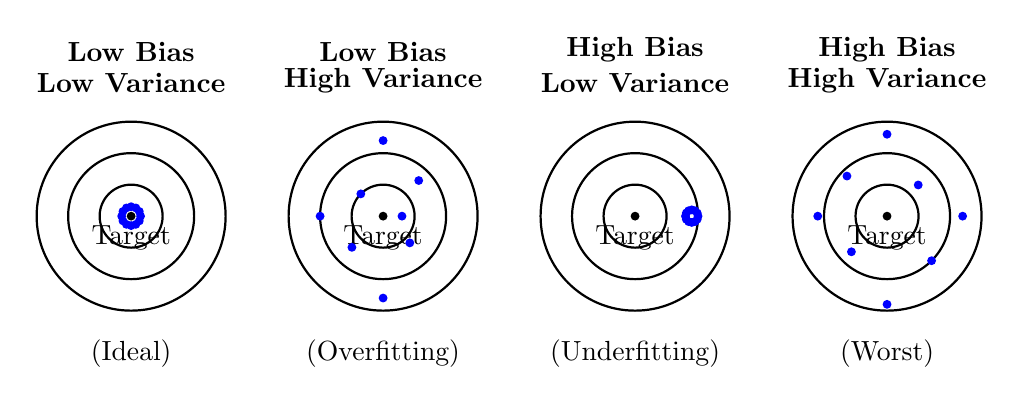
\begin{tikzpicture}[scale=0.8]
% Low Bias, Low Variance
    \begin{scope}[shift={(0,0)}]
        \draw[thick] (0,0) circle (1.5);
        \draw[thick] (0,0) circle (1.0);
        \draw[thick] (0,0) circle (0.5);
        \fill (0,0) circle (2pt) node[below] {Target};
        \foreach \a in {0,30,60,...,330} {
            \fill[blue] ({0.15*cos(\a)}, {0.15*sin(\a)}) circle (2pt);
        }
        \node[above] at (0, 2.3) {\textbf{Low Bias}};
        \node[above] at (0, 1.8) {\textbf{Low Variance}};
        \node[below] at (0, -1.8) {(Ideal)};
    \end{scope}
% Low Bias, High Variance
    \begin{scope}[shift={(4,0)}]
        \draw[thick] (0,0) circle (1.5);
        \draw[thick] (0,0) circle (1.0);
        \draw[thick] (0,0) circle (0.5);
        \fill (0,0) circle (2pt) node[below] {Target};
        \foreach \a/\r in {0/0.3, 45/0.8, 90/1.2, 135/0.5, 180/1.0, 225/0.7, 270/1.3, 315/0.6} {
            \fill[blue] ({{\r*cos(\a)}}, {{\r*sin(\a)}}) circle (2pt);
        }
        \node[above] at (0, 2.3) {\textbf{Low Bias}};
        \node[above] at (0, 1.8) {\textbf{High Variance}};
        \node[below] at (0, -1.8) {(Overfitting)};
    \end{scope}
% High Bias, Low Variance
    \begin{scope}[shift={(8,0)}]
        \draw[thick] (0,0) circle (1.5);
        \draw[thick] (0,0) circle (1.0);
        \draw[thick] (0,0) circle (0.5);
        \fill (0,0) circle (2pt) node[below] {Target};
        \foreach \a in {0,30,60,...,330} {
            \fill[blue] ({0.9 + 0.1*cos(\a)}, {0.1*sin(\a)}) circle (2pt);
        }
        \node[above] at (0, 2.3) {\textbf{High Bias}};
        \node[above] at (0, 1.8) {\textbf{Low Variance}};
        \node[below] at (0, -1.8) {(Underfitting)};
    \end{scope}
% High Bias, High Variance
    \begin{scope}[shift={(12,0)}]
        \draw[thick] (0,0) circle (1.5);
        \draw[thick] (0,0) circle (1.0);
        \draw[thick] (0,0) circle (0.5);
        \fill (0,0) circle (2pt) node[below] {Target};
        \foreach \a/\r in {0/0.7, 45/1.3, 90/0.9, 135/1.1, 180/0.8, 225/1.4, 270/1.0, 315/1.2} {
            \fill[blue] ({{\r*cos(\a + 45)}}, {{\r*sin(\a + 45)}}) circle (2pt);
        }
        \node[above] at (0, 2.3) {\textbf{High Bias}};
        \node[above] at (0, 1.8) {\textbf{High Variance}};
        \node[below] at (0, -1.8) {(Worst)};
    \end{scope}
\end{tikzpicture}
\end{center}

\textbf{Each dot:} Prediction from a model trained on different dataset

\textbf{Bullseye:} True function value

\textbf{Cluster center:} Average prediction across all datasets
\end{geometrybox}
\pagebreak
\begin{geometrybox}
\textbf{Error vs Model Complexity:}
\begin{center}
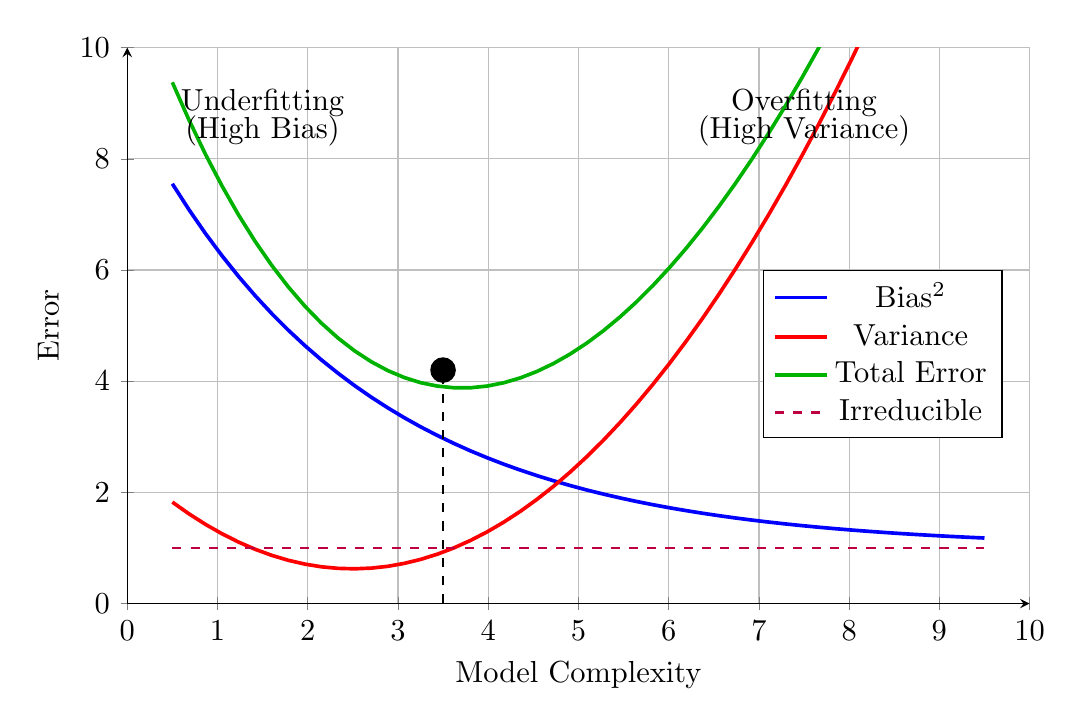
\begin{tikzpicture}[scale=1.1]
    \begin{axis}[
        axis lines = left,
        xlabel = {Model Complexity},
        ylabel = {Error},
        xmin=0, xmax=10,
        ymin=0, ymax=10,
        width=12cm,
        height=8cm,
        legend pos=north east,
        legend style={at={(0.97,0.60)}, anchor=north east},
        grid=major
    ]
% Bias^2 (decreasing)
    \addplot[blue, very thick, domain=0.5:9.5, samples=50] {8*exp(-0.4*x) + 1};
    \addlegendentry{Bias$^2$}
% Variance (increasing)
    \addplot[red, very thick, domain=0.5:9.5, samples=50] {0.3*x^2 - 1.5*x + 2.5};
    \addlegendentry{Variance}
% Total Error (U-shaped)
    \addplot[green!70!black, very thick, domain=0.5:9.5, samples=50] 
        {8*exp(-0.4*x) + 1 + 0.3*x^2 - 1.5*x + 2.5};
    \addlegendentry{Total Error}
% Irreducible Error (constant)
    \addplot[purple, thick, dashed, domain=0.5:9.5] {1};
    \addlegendentry{Irreducible}
% Optimal point
    \addplot[mark=*, only marks, mark size=4pt] coordinates {(3.5, 4.2)};
    \draw[dashed] (3.5, 0) -- (3.5, 4.2);
    \node[below] at (3.5, 0) {Optimal};
% Regions
    \node at (1.5, 9) {Underfitting};
    \node at (1.5, 8.5) {(High Bias)};
    \node at (7.5, 9) {Overfitting};
    \node at (7.5, 8.5) {(High Variance)};
    \end{axis}
\end{tikzpicture}
\end{center}

\textbf{Key observations:}
\begin{itemize}
    \item \textbf{Low complexity:} High bias, low variance → Underfitting
    \item \textbf{High complexity:} Low bias, high variance → Overfitting
    \item \textbf{Optimal:} Sweet spot minimizing total error
    \item \textbf{Trade-off:} Can't simultaneously minimize both bias and variance
\end{itemize}
\end{geometrybox}

\section{Examples Across Different Models}

\subsection{Polynomial Regression Example}

\begin{example}[Bias-Variance in Polynomial Regression]

\textbf{True function:} $f(x) = \sin(x) + \text{noise}$

\textbf{Model 1: Degree 1 (Linear)}
\begin{equation}
    \hat{f}(x) = \beta_0 + \beta_1 x
\end{equation}

\textbf{Analysis:}
\begin{itemize}
    \item \textbf{Bias:} HIGH - Linear can't capture sine wave
    \item \textbf{Variance:} LOW - Only 2 parameters, stable
    \item \textbf{Result:} Underfitting
\end{itemize}

\textbf{Model 2: Degree 3}
\begin{equation}
    \hat{f}(x) = \beta_0 + \beta_1 x + \beta_2 x^2 + \beta_3 x^3
\end{equation}

\textbf{Analysis:}
\begin{itemize}
    \item \textbf{Bias:} MEDIUM - Can approximate sine reasonably
    \item \textbf{Variance:} MEDIUM - 4 parameters, moderate flexibility
    \item \textbf{Result:} Good balance!
\end{itemize}

\textbf{Model 3: Degree 15}
\begin{equation}
    \hat{f}(x) = \beta_0 + \beta_1 x + \cdots + \beta_{15} x^{15}
\end{equation}

\textbf{Analysis:}
\begin{itemize}
    \item \textbf{Bias:} LOW - Can fit almost any function
    \item \textbf{Variance:} HIGH - 16 parameters, very sensitive
    \item \textbf{Result:} Overfitting - wiggles between data points
\end{itemize}

\textbf{Numerical Example:}

Suppose after training on 10 different datasets:

\begin{center}
\begin{tabular}{|c|c|c|c|}
\hline
Model & Bias$^2$ & Variance & Total Error \\
\hline
Degree 1 & 5.2 & 0.3 & 6.5 \\
Degree 3 & 0.8 & 1.2 & 3.0 ← Best \\
Degree 15 & 0.1 & 8.7 & 9.8 \\
\hline
\end{tabular}
\end{center}

(Assuming irreducible error = 1.0)
\end{example}

\subsection{k-NN Example}

\begin{example}[Bias-Variance in k-NN]

\textbf{k = 1 (1-Nearest Neighbor):}
\begin{itemize}
    \item \textbf{Bias:} LOW - Decision boundary very flexible
    \item \textbf{Variance:} HIGH - Prediction changes dramatically with different samples
    \item \textbf{Training error:} 0 (memorizes training data)
    \item \textbf{Test error:} HIGH (overfitting)
\end{itemize}

\textbf{k = 5:}
\begin{itemize}
    \item \textbf{Bias:} MEDIUM - Averages over 5 neighbors
    \item \textbf{Variance:} MEDIUM - More stable than k=1
    \item \textbf{Result:} Good balance
\end{itemize}

\textbf{k = n (all points):}
\begin{itemize}
    \item \textbf{Bias:} HIGH - Always predicts overall mean/mode
    \item \textbf{Variance:} LOW - Same prediction regardless of sample
    \item \textbf{Result:} Severe underfitting
\end{itemize}

\textbf{Pattern:} As $k$ increases, bias ↑ and variance ↓
\end{example}

\subsection{Decision Tree Example}

\begin{example}[Bias-Variance in Decision Trees]

\textbf{max\_depth = 1 (Decision Stump):}
\begin{itemize}
    \item \textbf{Bias:} HIGH - Can only make one split
    \item \textbf{Variance:} LOW - Very simple, stable
    \item \textbf{Result:} Underfitting
\end{itemize}

\textbf{max\_depth = 5:}
\begin{itemize}
    \item \textbf{Bias:} MEDIUM - Can capture moderate complexity
    \item \textbf{Variance:} MEDIUM - Reasonably stable
    \item \textbf{Result:} Often optimal
\end{itemize}

\textbf{max\_depth = $\infty$ (Full tree):}
\begin{itemize}
    \item \textbf{Bias:} LOW - Can perfectly fit training data
    \item \textbf{Variance:} HIGH - Different samples → completely different trees
    \item \textbf{Result:} Severe overfitting
\end{itemize}

\textbf{Why trees have high variance:}
\begin{itemize}
    \item Small change in data → Different top split → Completely different tree
    \item Hierarchical structure amplifies small changes
    \item This is why ensemble methods (Random Forests) help!
\end{itemize}
\end{example}

\subsection{Ridge Regression Example}

\begin{example}[Bias-Variance in Ridge Regression]

Recall: Ridge minimizes $\frac{1}{2}||\mathbf{y} - \mathbf{X}\boldsymbol{\beta}||^2 + \lambda||\boldsymbol{\beta}||^2$

\textbf{$\lambda = 0$ (OLS):}
\begin{itemize}
    \item \textbf{Bias:} LOW - No constraint on coefficients
    \item \textbf{Variance:} HIGH (especially with multicollinearity)
    \item \textbf{Coefficients:} Large magnitudes possible
\end{itemize}

\textbf{$\lambda = 1$ (Small penalty):}
\begin{itemize}
    \item \textbf{Bias:} SLIGHTLY INCREASED - Small shrinkage
    \item \textbf{Variance:} REDUCED - More stable estimates
    \item \textbf{Result:} Often better than OLS
\end{itemize}

\textbf{$\lambda = 100$ (Large penalty):}
\begin{itemize}
    \item \textbf{Bias:} HIGH - Heavy shrinkage toward zero
    \item \textbf{Variance:} VERY LOW - Very stable
    \item \textbf{Result:} May underfit
\end{itemize}

\textbf{$\lambda = \infty$:}
\begin{itemize}
    \item \textbf{Bias:} MAXIMUM - All $\beta_j = 0$
    \item \textbf{Variance:} ZERO - No randomness
    \item \textbf{Result:} Just predicts mean (useless!)
\end{itemize}

\textbf{Pattern:} As $\lambda$ increases, bias ↑ and variance ↓
\end{example}

\section{Model Complexity and Generalization}

\begin{definition}[Model Complexity]
\textbf{Model complexity} refers to the flexibility or capacity of a model:

\textbf{Increases with:}
\begin{itemize}
    \item More parameters (polynomial degree, number of features)
    \item Less regularization (smaller $\lambda$)
    \item More flexibility (deeper trees, smaller k in k-NN)
\end{itemize}

\textbf{Measures of complexity:}
\begin{itemize}
    \item Number of parameters
    \item VC dimension (theoretical)
    \item Effective degrees of freedom
\end{itemize}
\end{definition}

\begin{theorem}[Fundamental Trade-off]
\textbf{Simple models (Low complexity):}
\begin{equation}
    \text{High Bias, Low Variance} \to \text{Underfitting}
\end{equation}

\textbf{Complex models (High complexity):}
\begin{equation}
    \text{Low Bias, High Variance} \to \text{Overfitting}
\end{equation}

\textbf{Goal:} Find the sweet spot that minimizes total error!
\end{theorem}

\section{Diagnosing Bias vs Variance Problems}

\begin{importantbox}
\textbf{How to identify if you have bias or variance issues:}

\textbf{High Bias (Underfitting):}
\begin{itemize}
    \item Training error is HIGH
    \item Training error $\approx$ Test error (small gap)
    \item Model performs poorly on both training and test
    \item Learning curves plateau early (more data doesn't help much)
\end{itemize}

\textbf{High Variance (Overfitting):}
\begin{itemize}
    \item Training error is LOW
    \item Test error >> Training error (large gap)
    \item Model performs well on training but poorly on test
    \item Learning curves show large gap that persists
\end{itemize}

\textbf{Good Fit:}
\begin{itemize}
    \item Training error is reasonable
    \item Small gap between training and test error
    \item Both errors are acceptable for the problem
\end{itemize}
\end{importantbox}

\begin{geometrybox}
\textbf{Learning Curves:}

\begin{center}
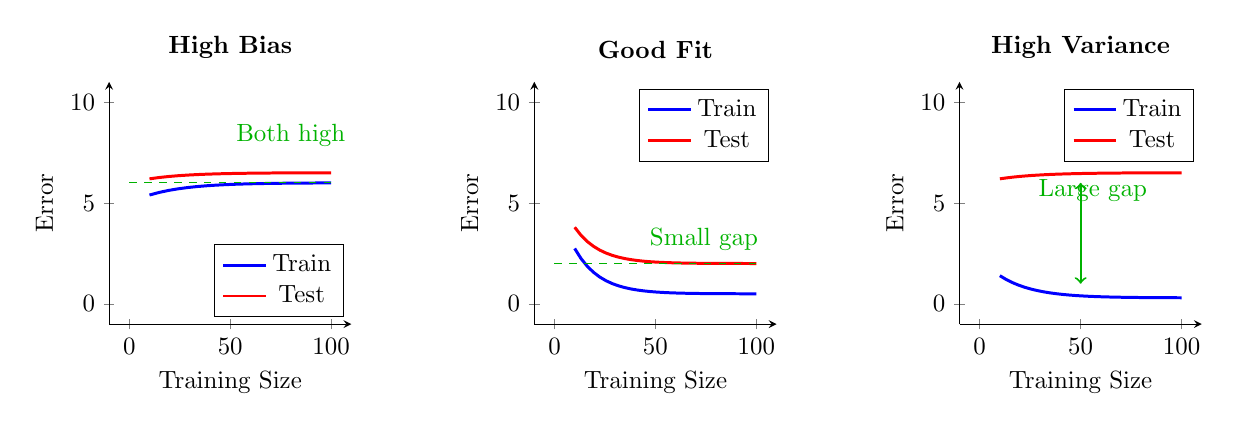
\begin{tikzpicture}[scale=0.9]

% =========================
% High Bias
% =========================
\begin{scope}[shift={(0,0)}]
\begin{axis}[
    axis lines = left,
    xlabel = {Training Size},
    ylabel = {Error},
    xmin=0, xmax=100,
    ymin=0, ymax=10,
    width=5cm,
    height=5cm,
    title={\textbf{High Bias}},
    legend pos=south east,
    clip=false,
    enlargelimits=0.1
]
\addplot[blue, very thick, domain=10:100, samples=20]
    {6 - 1*exp(-0.05*x)};
\addlegendentry{Train}

\addplot[red, very thick, domain=10:100, samples=20]
    {6.5 - 0.5*exp(-0.05*x)};
\addlegendentry{Test}

\draw[dashed, green!70!black]
    (axis cs:0,6) -- (axis cs:100,6);

\node[green!70!black]
    at (axis description cs:0.75,0.78)
    {Both high};

\end{axis}
\end{scope}

% =========================
% Good Fit
% =========================
\begin{scope}[shift={(6,0)}]
\begin{axis}[
    axis lines = left,
    xlabel = {Training Size},
    ylabel = {Error},
    xmin=0, xmax=100,
    ymin=0, ymax=10,
    width=5cm,
    height=5cm,
    title={\textbf{Good Fit}},
    legend pos=north east,
    clip=false,
    enlargelimits=0.1
]
\addplot[blue, very thick, domain=10:100, samples=30]
    {0.5 + 5*exp(-0.08*x)};
\addlegendentry{Train}

\addplot[red, very thick, domain=10:100, samples=30]
    {2 + 4*exp(-0.08*x)};
\addlegendentry{Test}

\draw[dashed, green!70!black]
    (axis cs:0,2) -- (axis cs:100,2);

\node[green!70!black]
    at (axis description cs:0.70,0.35)
    {Small gap};

\end{axis}
\end{scope}

% =========================
% High Variance
% =========================
\begin{scope}[shift={(12,0)}]
\begin{axis}[
    axis lines = left,
    xlabel = {Training Size},
    ylabel = {Error},
    xmin=0, xmax=100,
    ymin=0, ymax=10,
    width=5cm,
    height=5cm,
    title={\textbf{High Variance}},
    legend pos=north east,
    clip=false,
    enlargelimits=0.1
]
\addplot[blue, very thick, domain=10:100, samples=30]
    {0.3 + 2*exp(-0.06*x)};
\addlegendentry{Train}

\addplot[red, very thick, domain=10:100, samples=30]
    {6.5 - 0.5*exp(-0.05*x)};
\addlegendentry{Test}

\draw[<->, green!70!black, thick]
    (axis cs:50,1) -- (axis cs:50,6);

\node[green!70!black]
    at (axis description cs:0.55,0.55)
    {Large gap};

\end{axis}
\end{scope}

\end{tikzpicture}
\end{center}

\textbf{Interpretation:}
\begin{itemize}
    \item \textbf{High Bias:} Both curves plateau at high error
    \item \textbf{Good Fit:} Curves converge at acceptable error
    \item \textbf{High Variance:} Large persistent gap between curves
\end{itemize}
\end{geometrybox}

\section{Remedies for Bias and Variance}

\begin{importantbox}
\textbf{If you have HIGH BIAS (Underfitting):}

\begin{enumerate}
    \item \textbf{Increase model complexity:}
    \begin{itemize}
        \item Add more features or polynomial terms
        \item Increase tree depth
        \item Decrease regularization ($\lambda$)
        \item Use more complex model (e.g., neural network instead of linear)
    \end{itemize}
    
    \item \textbf{Feature engineering:}
    \begin{itemize}
        \item Create interaction terms
        \item Add domain-specific features
        \item Transform features (log, sqrt, etc.)
    \end{itemize}
    
    \item \textbf{Reduce constraints:}
    \begin{itemize}
        \item Remove regularization
        \item Remove feature selection that may be too aggressive
    \end{itemize}
    
    \item \textbf{Note:} More training data usually won't help much!
\end{enumerate}

\textbf{If you have HIGH VARIANCE (Overfitting):}

\begin{enumerate}
    \item \textbf{Get more training data:}
    \begin{itemize}
        \item Most effective if feasible
        \item Reduces variance directly
    \end{itemize}
    
    \item \textbf{Reduce model complexity:}
    \begin{itemize}
        \item Remove features (feature selection)
        \item Reduce polynomial degree
        \item Limit tree depth (max\_depth)
        \item Increase k in k-NN
    \end{itemize}
    
    \item \textbf{Add regularization:}
    \begin{itemize}
        \item Increase $\lambda$ in Ridge/Lasso
        \item Add dropout in neural networks
        \item Use early stopping
    \end{itemize}
    
    \item \textbf{Use ensemble methods:}
    \begin{itemize}
        \item Bagging/Random Forests reduce variance
        \item Averaging multiple models
    \end{itemize}
    
    \item \textbf{Cross-validation:}
    \begin{itemize}
        \item Use k-fold CV to tune hyperparameters
        \item Prevents overfitting to validation set
    \end{itemize}
\end{enumerate}
\end{importantbox}

\section{Cross-Validation: The Solution to Model Selection}

\begin{definition}[Cross-Validation Purpose]
\textbf{Goal:} Estimate how well a model will generalize to independent data.

\textbf{Why needed:}
\begin{itemize}
    \item Training error is too optimistic (always decreases with complexity)
    \item Single test set may not be representative
    \item Limited data - want to use all of it for both training and evaluation
\end{itemize}

\textbf{Idea:} Split data multiple ways, train and test on each split, average results.
\end{definition}

\subsection{Holdout Method (Baseline)}

\begin{definition}[Simple Train-Test Split]
\textbf{Algorithm:}
\begin{enumerate}
    \item Split data: 70-80\% training, 20-30\% test
    \item Train model on training set
    \item Evaluate on test set
    \item Report test error as estimate of generalization error
\end{enumerate}

\textbf{Advantages:}
\begin{itemize}
    \item Simple, fast
    \item Test set completely independent
\end{itemize}

\textbf{Disadvantages:}
\begin{itemize}
    \item Wastes data (test set not used for training)
    \item High variance (depends on particular split)
    \item Not suitable for small datasets
\end{itemize}
\end{definition}

\subsection{Leave-One-Out Cross-Validation (LOOCV)}

\begin{definition}[LOOCV Algorithm]
For a dataset with $n$ samples:

\textbf{Algorithm:}
\begin{enumerate}
    \item For $i = 1$ to $n$:
    \begin{enumerate}
        \item Use sample $i$ as test set (1 sample)
        \item Use remaining $n-1$ samples as training set
        \item Train model and compute error on sample $i$: $\text{Err}_i$
    \end{enumerate}
    \item Average all errors:
    \begin{equation}
        \text{CV}_{\text{LOOCV}} = \frac{1}{n}\sum_{i=1}^{n}\text{Err}_i
    \end{equation}
\end{enumerate}

\textbf{Advantages:}
\begin{itemize}
    \item Uses maximum data for training ($n-1$ samples)
    \item Deterministic (no randomness in splits)
    \item Nearly unbiased estimate of test error
\end{itemize}

\textbf{Disadvantages:}
\begin{itemize}
    \item Computationally expensive (train $n$ times!)
    \item High variance (test sets overlap heavily)
    \item Training sets are very similar → correlated errors
\end{itemize}
\end{definition}

\begin{example}[LOOCV Calculation]

\textbf{Dataset:} 5 samples

\begin{center}
\begin{tabular}{|c|c|c|c|}
\hline
Iteration & Training Set & Test Set & Error \\
\hline
1 & \{2,3,4,5\} & \{1\} & 0.5 \\
2 & \{1,3,4,5\} & \{2\} & 0.3 \\
3 & \{1,2,4,5\} & \{3\} & 0.8 \\
4 & \{1,2,3,5\} & \{4\} & 0.4 \\
5 & \{1,2,3,4\} & \{5\} & 0.6 \\
\hline
\end{tabular}
\end{center}

\textbf{LOOCV Error:}
\begin{equation}
    \text{CV}_{\text{LOOCV}} = \frac{0.5 + 0.3 + 0.8 + 0.4 + 0.6}{5} = \frac{2.6}{5} = 0.52
\end{equation}
\end{example}

\subsection{k-Fold Cross-Validation}

\begin{definition}[k-Fold CV Algorithm]
\textbf{Algorithm:}
\begin{enumerate}
    \item Randomly partition data into $k$ equal-sized folds
    \item For $i = 1$ to $k$:
    \begin{enumerate}
        \item Use fold $i$ as test set
        \item Use remaining $k-1$ folds as training set
        \item Train model and compute error on fold $i$: $\text{Err}_i$
    \end{enumerate}
    \item Average all errors:
    \begin{equation}
        \text{CV}_{k} = \frac{1}{k}\sum_{i=1}^{k}\text{Err}_i
    \end{equation}
\end{enumerate}

\textbf{Common choices:}
\begin{itemize}
    \item $k = 5$: Good balance of bias and variance
    \item $k = 10$: Most common in practice
    \item $k = n$: Equivalent to LOOCV
\end{itemize}

\textbf{Advantages:}
\begin{itemize}
    \item Computational efficient (only $k$ iterations)
    \item Lower variance than LOOCV
    \item Good bias-variance trade-off
    \item Uses all data for both training and testing
\end{itemize}

\textbf{Disadvantages:}
\begin{itemize}
    \item Slightly more biased than LOOCV (trains on less data)
    \item Results depend on random partition
    \item Still relatively expensive for large datasets
\end{itemize}
\end{definition}

\begin{example}[5-Fold CV Calculation]

\textbf{Dataset:} 100 samples, split into 5 folds of 20 samples each

\begin{center}
\begin{tabular}{|c|c|c|c|}
\hline
Fold & Training Set Size & Test Set Size & Error \\
\hline
1 & 80 (folds 2,3,4,5) & 20 (fold 1) & 0.15 \\
2 & 80 (folds 1,3,4,5) & 20 (fold 2) & 0.12 \\
3 & 80 (folds 1,2,4,5) & 20 (fold 3) & 0.18 \\
4 & 80 (folds 1,2,3,5) & 20 (fold 4) & 0.14 \\
5 & 80 (folds 1,2,3,4) & 20 (fold 5) & 0.16 \\
\hline
\end{tabular}
\end{center}

\textbf{5-Fold CV Error:}
\begin{equation}
    \text{CV}_{5} = \frac{0.15 + 0.12 + 0.18 + 0.14 + 0.16}{5} = \frac{0.75}{5} = 0.15
\end{equation}

\textbf{Also compute standard deviation:}
\begin{equation}
    \text{SD} = \sqrt{\frac{\sum_{i=1}^{5}(\text{Err}_i - 0.15)^2}{5}} \approx 0.02
\end{equation}

This gives us: $\text{CV} = 0.15 \pm 0.02$ (confidence in estimate)
\end{example}

\subsection{Stratified k-Fold CV}

\begin{definition}[Stratified k-Fold]
\textbf{Modification for classification:}

Ensure each fold has approximately the same class distribution as the full dataset.

\textbf{Why needed:}
\begin{itemize}
    \item Prevents folds with very different class ratios
    \item Especially important for imbalanced datasets
    \item Reduces variance of CV estimate
\end{itemize}

\textbf{Example:} If dataset is 70\% Class A, 30\% Class B:
\begin{itemize}
    \item Regular k-fold: Some folds might be 80-20, others 60-40
    \item Stratified k-fold: All folds are approximately 70-30
\end{itemize}

\textbf{Best practice:} Always use stratified k-fold for classification!
\end{definition}

\section{Using Cross-Validation for Model Selection}

\begin{definition}[Hyperparameter Tuning with CV]

\textbf{Problem:} Choose optimal hyperparameters (e.g., $\lambda$ for ridge, k for k-NN)

\textbf{Algorithm:}
\begin{enumerate}
    \item Define grid of hyperparameter values to try
    \item For each hyperparameter combination:
    \begin{enumerate}
        \item Perform k-fold CV
        \item Compute average CV error
    \end{enumerate}
    \item Select hyperparameters with lowest CV error
    \item Retrain on full training set with chosen hyperparameters
    \item Evaluate on independent test set
\end{enumerate}

\textbf{Important:} Test set should NEVER be used for hyperparameter selection!
\end{definition}

\begin{example}[Ridge Regression Hyperparameter Tuning]

\textbf{Task:} Choose optimal $\lambda$ for ridge regression

\textbf{Candidates:} $\lambda \in \{0.01, 0.1, 1, 10, 100\}$

\textbf{Using 10-fold CV:}

\begin{center}
\begin{tabular}{|c|c|}
\hline
$\lambda$ & 10-Fold CV Error \\
\hline
0.01 & 12.5 \\
0.1 & 10.8 \\
1.0 & 9.2 ← \textbf{Best!} \\
10.0 & 11.3 \\
100.0 & 15.7 \\
\hline
\end{tabular}
\end{center}

\textbf{Decision:} Choose $\lambda = 1.0$

\textbf{Final step:} Retrain on full training set with $\lambda = 1.0$, evaluate on test set.
\end{example}

\section{Bias-Variance Trade-off in Cross-Validation}

\begin{theorem}[Bias-Variance of CV Estimates]

\textbf{LOOCV:}
\begin{itemize}
    \item \textbf{Bias:} Nearly unbiased (trains on $n-1$ samples)
    \item \textbf{Variance:} High (test sets overlap, correlated estimates)
\end{itemize}

\textbf{k-Fold CV:}
\begin{itemize}
    \item \textbf{Bias:} Slightly biased upward (trains on less data than LOOCV)
    \item \textbf{Variance:} Lower (less overlap between test sets)
\end{itemize}

\textbf{Trade-off:}
\begin{itemize}
    \item Larger $k$ → Lower bias, higher variance
    \item Smaller $k$ → Higher bias, lower variance
    \item $k = 10$ often optimal balance
\end{itemize}
\end{theorem}

\section{GATE-Style Problems}

\begin{example}[Problem 1: Identifying Bias vs Variance]

\textbf{Given:}
\begin{itemize}
    \item Model A: Training error = 2\%, Test error = 15\%
    \item Model B: Training error = 15\%, Test error = 16\%
\end{itemize}

\textbf{Question:} Which model has high bias? High variance?

\textbf{Solution:}

\textbf{Model A:}
\begin{itemize}
    \item Training error is very low (2\%)
    \item Large gap: Test - Train = 13\%
    \item \textbf{Diagnosis: High Variance (Overfitting)}
\end{itemize}

\textbf{Model B:}
\begin{itemize}
    \item Training error is high (15\%)
    \item Small gap: Test - Train = 1\%
    \item Both errors are high
    \item \textbf{Diagnosis: High Bias (Underfitting)}
\end{itemize}
\end{example}

\begin{example}[Problem 2: LOOCV Calculation]

\textbf{Dataset:} 4 samples with true values $y = [2, 4, 6, 8]$

\textbf{Model:} Predicts mean of training set

\textbf{Calculate LOOCV error.}

\textbf{Solution:}

\textbf{Iteration 1:} Train on \{4,6,8\}, test on \{2\}
\begin{equation}
    \text{Prediction} = \frac{4+6+8}{3} = 6, \quad \text{Error} = (2-6)^2 = 16
\end{equation}

\textbf{Iteration 2:} Train on \{2,6,8\}, test on \{4\}
\begin{equation}
    \text{Prediction} = \frac{2+6+8}{3} = 5.33, \quad \text{Error} = (4-5.33)^2 \approx 1.78
\end{equation}

\textbf{Iteration 3:} Train on \{2,4,8\}, test on \{6\}
\begin{equation}
    \text{Prediction} = \frac{2+4+8}{3} = 4.67, \quad \text{Error} = (6-4.67)^2 \approx 1.78
\end{equation}

\textbf{Iteration 4:} Train on \{2,4,6\}, test on \{8\}
\begin{equation}
    \text{Prediction} = \frac{2+4+6}{3} = 4, \quad \text{Error} = (8-4)^2 = 16
\end{equation}

\textbf{LOOCV Error:}
\begin{equation}
    \text{CV} = \frac{16 + 1.78 + 1.78 + 16}{4} = \frac{35.56}{4} = 8.89
\end{equation}
\end{example}

\begin{example}[Problem 3: Bias-Variance Trade-off]

\textbf{Question:} For polynomial regression, what happens to bias and variance as degree increases from 1 to 20?

\textbf{Answer:}

\textbf{As degree increases:}
\begin{itemize}
    \item \textbf{Bias:} Decreases (model becomes more flexible)
    \item \textbf{Variance:} Increases (more parameters, more sensitivity)
    \item \textbf{Training error:} Decreases (better fit)
    \item \textbf{Test error:} First decreases, then increases (U-shaped)
\end{itemize}

\textbf{Optimal degree:} Where test error is minimized (balance of bias and variance)
\end{example}

\section{Summary - Key Points for GATE}

\begin{importantbox}
\textbf{Must Know for GATE:}

\begin{enumerate}
    \item \textbf{Bias-Variance Decomposition:}
    \begin{equation}
        \text{Error} = \text{Bias}^2 + \text{Variance} + \text{Irreducible}
    \end{equation}
    
    \item \textbf{Bias:}
    \begin{itemize}
        \item Error from wrong model assumptions
        \item High bias → Underfitting
        \item Both training and test errors high
        \item Fix: Increase model complexity
    \end{itemize}
    
    \item \textbf{Variance:}
    \begin{itemize}
        \item Error from sensitivity to training data
        \item High variance → Overfitting
        \item Low training error, high test error (large gap)
        \item Fix: Get more data, reduce complexity, regularize
    \end{itemize}
    
    \item \textbf{Trade-off:}
    \begin{itemize}
        \item Cannot minimize both simultaneously
        \item Simple models: High bias, low variance
        \item Complex models: Low bias, high variance
        \item Goal: Find optimal complexity
    \end{itemize}
    
    \item \textbf{Model Complexity Effects:}
    \begin{itemize}
        \item Increasing: Polynomial degree, tree depth, k in k-NN (inverse), number of features
        \item Decreasing: Regularization ($\lambda$), pruning, feature selection
    \end{itemize}
    
    \item \textbf{Cross-Validation:}
    \begin{itemize}
        \item LOOCV: $n$ iterations, nearly unbiased, high variance
        \item k-Fold: $k$ iterations (typically 5 or 10), balanced
        \item Stratified: Maintains class distribution in each fold
    \end{itemize}
    
    \item \textbf{CV Formulas:}
    \begin{align}
        \text{CV}_{\text{LOOCV}} &= \frac{1}{n}\sum_{i=1}^{n}\text{Err}_i \\
        \text{CV}_{k} &= \frac{1}{k}\sum_{i=1}^{k}\text{Err}_i
    \end{align}
    
    \item \textbf{Learning Curves:}
    \begin{itemize}
        \item High bias: Both curves plateau at high error
        \item High variance: Large gap between training and test
        \item Good fit: Small gap, acceptable error
    \end{itemize}
    
    \item \textbf{Use CV for:}
    \begin{itemize}
        \item Hyperparameter tuning
        \item Model selection
        \item Estimating generalization error
    \end{itemize}
    
    \item \textbf{Never use test set for:}
    \begin{itemize}
        \item Hyperparameter selection
        \item Model comparison
        \item Any training decision
    \end{itemize}
\end{enumerate}
\end{importantbox}

\begin{gatepoint}
\textbf{Common GATE Question Types:}

\begin{enumerate}
    \item Identify whether model has high bias or variance from training/test errors
    \item Explain bias-variance decomposition
    \item Calculate LOOCV or k-fold CV error by hand
    \item Understand effect of model complexity on bias/variance
    \item Know how to fix underfitting vs overfitting
    \item Interpret learning curves
    \item Compare LOOCV vs k-fold CV
    \item Understand stratified CV
    \item Know when to use which CV method
    \item Explain irreducible error
    \item Understand why test set must be independent
    \item Know hyperparameter tuning process with CV
\end{enumerate}
\end{gatepoint}
\chapter{Multi-Layer Perceptron and Feed-Forward Neural Networks}

\section{Introduction to Neural Networks}

\begin{mentalmodel}
Imagine your brain making a decision:

\textbf{Simple decision (Linear):}
\begin{itemize}
    \item "If price < \$100 AND quality > 7, then buy"
    \item Single yes/no rule
    \item Like logistic regression
\end{itemize}

\textbf{Complex decision (Neural Network):}
\begin{itemize}
    \item Multiple intermediate thoughts/features
    \item "Is it affordable?" (combines price and budget)
    \item "Is it worthwhile?" (combines quality and reviews)
    \item "Do I need it?" (combines urgency and existing items)
    \item Final decision: Combine all these intermediate conclusions
\end{itemize}

\textbf{Neural networks work the same way!}

Build complex decisions from layers of simpler decisions.
\end{mentalmodel}

\begin{keyidea}
A \textbf{Multi-Layer Perceptron (MLP)} is a feed-forward artificial neural network consisting of:

\begin{enumerate}
    \item \textbf{Input layer:} Receives features
    \item \textbf{Hidden layer(s):} Intermediate computations that learn representations
    \item \textbf{Output layer:} Makes final predictions
\end{enumerate}

\textbf{Key properties:}
\begin{itemize}
    \item \textbf{Feed-forward:} Information flows in one direction (input → output)
    \item \textbf{Fully connected:} Each neuron connects to all neurons in next layer
    \item \textbf{Non-linear:} Uses activation functions to capture complex patterns
    \item \textbf{Universal approximator:} Can approximate any continuous function (with enough neurons)
\end{itemize}

\textbf{Why "Perceptron"?} The basic building block (artificial neuron) is called a perceptron.
\end{keyidea}

\section{The Artificial Neuron (Perceptron)}

\subsection{Single Neuron Structure}

\begin{definition}[Artificial Neuron]
An artificial neuron receives multiple inputs, computes a weighted sum, adds a bias, and applies an activation function:

\textbf{Components:}
\begin{itemize}
    \item \textbf{Inputs:} $x_1, x_2, \ldots, x_p$
    \item \textbf{Weights:} $w_1, w_2, \ldots, w_p$
    \item \textbf{Bias:} $b$
    \item \textbf{Activation function:} $\sigma(\cdot)$
\end{itemize}

\textbf{Computation:}
\begin{align}
    z &= w_1 x_1 + w_2 x_2 + \cdots + w_p x_p + b = \mathbf{w}^T\mathbf{x} + b \\
    a &= \sigma(z)
\end{align}

where:
\begin{itemize}
    \item $z$: Pre-activation (weighted sum)
    \item $a$: Activation (output of neuron)
\end{itemize}
\end{definition}

\begin{geometrybox}
\textbf{Single Neuron Diagram:}

\begin{center}
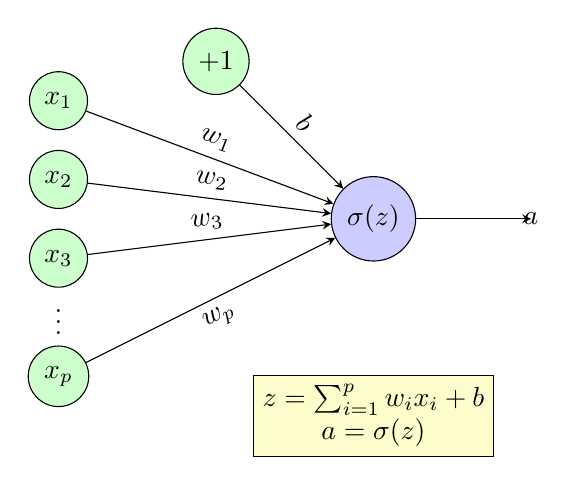
\begin{tikzpicture}[
    neuron/.style={circle, draw, minimum size=1cm, fill=blue!20},
    input/.style={circle, draw, minimum size=0.7cm, fill=green!20},
    >=stealth
]
    % Input nodes
    \node[input] (x1) at (0, 2) {$x_1$};
    \node[input] (x2) at (0, 1) {$x_2$};
    \node[input] (x3) at (0, 0) {$x_3$};
    \node at (0, -0.7) {$\vdots$};
    \node[input] (xp) at (0, -1.5) {$x_p$};
    
    % Neuron
    \node[neuron] (neuron) at (4, 0.5) {$\sigma(z)$};
    
    % Output
    \node at (6, 0.5) {$a$};
    
    % Connections with weights
    \draw[->] (x1) -- (neuron) node[midway, above, sloped] {$w_1$};
    \draw[->] (x2) -- (neuron) node[midway, above, sloped] {$w_2$};
    \draw[->] (x3) -- (neuron) node[midway, above, sloped] {$w_3$};
    \draw[->] (xp) -- (neuron) node[midway, below, sloped] {$w_p$};
    
    % Bias
    \node[input] (bias) at (2, 2.5) {$+1$};
    \draw[->] (bias) -- (neuron) node[midway, above, sloped] {$b$};
    
    % Output arrow
    \draw[->] (neuron) -- (6, 0.5);
    
    % Computation box
    \node[draw, rectangle, fill=yellow!20, align=center] at (4, -2) {
        $z = \sum_{i=1}^{p} w_i x_i + b$ \\
        $a = \sigma(z)$
    };
\end{tikzpicture}
\end{center}

\textbf{Think of it as:} The neuron "listens" to all inputs with different strengths (weights), combines them, and "decides" how much to activate based on the result.
\end{geometrybox}

\subsection{Activation Functions}

\begin{definition}[Common Activation Functions]

\textbf{1. Sigmoid (Logistic):}
\begin{equation}
    \sigma(z) = \frac{1}{1 + e^{-z}}
\end{equation}

\textbf{Properties:}
\begin{itemize}
    \item Range: $(0, 1)$
    \item Smooth, differentiable
    \item Derivative: $\sigma'(z) = \sigma(z)(1 - \sigma(z))$
    \item \textbf{Problem:} Vanishing gradients for large $|z|$
\end{itemize}

\textbf{2. Hyperbolic Tangent (tanh):}
\begin{equation}
    \tanh(z) = \frac{e^z - e^{-z}}{e^z + e^{-z}} = \frac{e^{2z} - 1}{e^{2z} + 1}
\end{equation}

\textbf{Properties:}
\begin{itemize}
    \item Range: $(-1, 1)$
    \item Zero-centered (better than sigmoid)
    \item Derivative: $\tanh'(z) = 1 - \tanh^2(z)$
    \item \textbf{Problem:} Still suffers from vanishing gradients
\end{itemize}

\textbf{3. ReLU (Rectified Linear Unit):}
\begin{equation}
    \text{ReLU}(z) = \max(0, z) = \begin{cases}
        z & \text{if } z > 0 \\
        0 & \text{if } z \leq 0
    \end{cases}
\end{equation}

\textbf{Properties:}
\begin{itemize}
    \item Range: $[0, \infty)$
    \item Derivative: $\begin{cases} 1 & \text{if } z > 0 \\ 0 & \text{if } z \leq 0 \end{cases}$
    \item \textbf{Advantages:} No vanishing gradient for $z > 0$, computationally efficient
    \item \textbf{Problem:} "Dying ReLU" - neurons can get stuck at 0
    \item \textbf{Most popular in practice!}
\end{itemize}

\textbf{4. Leaky ReLU:}
\begin{equation}
    \text{Leaky ReLU}(z) = \begin{cases}
        z & \text{if } z > 0 \\
        \alpha z & \text{if } z \leq 0
    \end{cases}
\end{equation}

where $\alpha$ is small (e.g., 0.01).

\textbf{Fixes dying ReLU problem!}

\textbf{5. Softmax (for multi-class output):}
\begin{equation}
    \text{softmax}(z_k) = \frac{e^{z_k}}{\sum_{j=1}^{K} e^{z_j}}
\end{equation}

Converts scores to probabilities that sum to 1.
\end{definition}

\begin{geometrybox}
\textbf{Activation Function Plots:}

\begin{center}
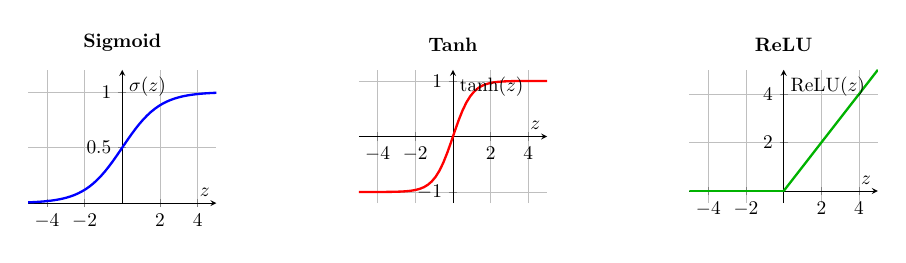
\begin{tikzpicture}[scale=0.7]
    % Sigmoid
    \begin{scope}[shift={(0,0)}]
        \begin{axis}[
            axis lines = center,
            xlabel = {$z$},
            ylabel = {$\sigma(z)$},
            ymin=0, ymax=1.2,
            xmin=-5, xmax=5,
            width=5cm,
            height=4cm,
            title={\textbf{Sigmoid}},
            grid=major
        ]
        \addplot[blue, very thick, domain=-5:5, samples=50] {1/(1+exp(-x))};
        \end{axis}
    \end{scope}
    
    % Tanh
    \begin{scope}[shift={(6,0)}]
        \begin{axis}[
            axis lines = center,
            xlabel = {$z$},
            ylabel = {$\tanh(z)$},
            ymin=-1.2, ymax=1.2,
            xmin=-5, xmax=5,
            width=5cm,
            height=4cm,
            title={\textbf{Tanh}},
            grid=major
        ]
        \addplot[red, very thick, domain=-5:5, samples=50] {tanh(x)};
        \end{axis}
    \end{scope}
    
    % ReLU
    \begin{scope}[shift={(12,0)}]
        \begin{axis}[
            axis lines = center,
            xlabel = {$z$},
            ylabel = {ReLU$(z)$},
            ymin=-0.5, ymax=5,
            xmin=-5, xmax=5,
            width=5cm,
            height=4cm,
            title={\textbf{ReLU}},
            grid=major
        ]
        \addplot[green!70!black, very thick, domain=-5:0] {0};
        \addplot[green!70!black, very thick, domain=0:5] {x};
        \end{axis}
    \end{scope}
\end{tikzpicture}
\end{center}
\end{geometrybox}

\begin{importantbox}
\textbf{Which activation function to use?}

\textbf{Hidden layers:}
\begin{itemize}
    \item \textbf{Default choice:} ReLU
    \item \textbf{Alternative:} Leaky ReLU (if dying ReLU is a problem)
    \item \textbf{Avoid:} Sigmoid, tanh (vanishing gradients in deep networks)
\end{itemize}

\textbf{Output layer:}
\begin{itemize}
    \item \textbf{Binary classification:} Sigmoid
    \item \textbf{Multi-class classification:} Softmax
    \item \textbf{Regression:} Linear (no activation) or ReLU (if outputs must be positive)
\end{itemize}
\end{importantbox}

\section{Multi-Layer Perceptron Architecture}

\begin{definition}[MLP Structure]
An MLP with $L$ layers consists of:

\textbf{Layer 0 (Input):} 
\begin{itemize}
    \item $\mathbf{a}^{[0]} = \mathbf{x}$ (input features)
    \item Dimension: $n_0 = p$ (number of features)
\end{itemize}

\textbf{Hidden Layers $\ell = 1, 2, \ldots, L-1$:}
\begin{align}
    \mathbf{z}^{[\ell]} &= \mathbf{W}^{[\ell]}\mathbf{a}^{[\ell-1]} + \mathbf{b}^{[\ell]} \\
    \mathbf{a}^{[\ell]} &= \sigma^{[\ell]}(\mathbf{z}^{[\ell]})
\end{align}

where:
\begin{itemize}
    \item $\mathbf{W}^{[\ell]}$: Weight matrix (size $n_\ell \times n_{\ell-1}$)
    \item $\mathbf{b}^{[\ell]}$: Bias vector (size $n_\ell$)
    \item $n_\ell$: Number of neurons in layer $\ell$
\end{itemize}

\textbf{Output Layer $L$:}
\begin{align}
    \mathbf{z}^{[L]} &= \mathbf{W}^{[L]}\mathbf{a}^{[L-1]} + \mathbf{b}^{[L]} \\
    \hat{\mathbf{y}} &= \sigma^{[L]}(\mathbf{z}^{[L]})
\end{align}
\end{definition}

\begin{geometrybox}
\textbf{3-Layer MLP (1 hidden layer):}

\begin{center}
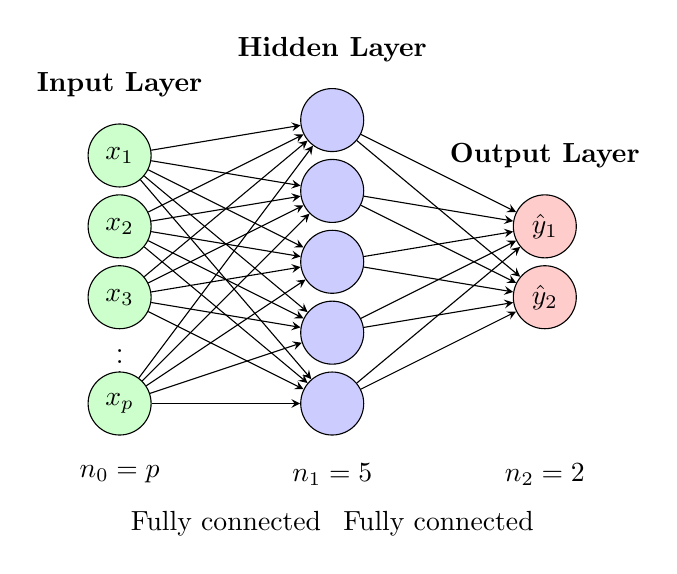
\begin{tikzpicture}[
    neuron/.style={circle, draw, minimum size=0.8cm, fill=blue!20},
    input/.style={circle, draw, minimum size=0.8cm, fill=green!20},
    output/.style={circle, draw, minimum size=0.8cm, fill=red!20},
    >=stealth,
    scale=0.9
]
    % Input layer
    \node[input] (i1) at (0, 3) {$x_1$};
    \node[input] (i2) at (0, 2) {$x_2$};
    \node[input] (i3) at (0, 1) {$x_3$};
    \node at (0, 0.2) {$\vdots$};
    \node[input] (ip) at (0, -0.5) {$x_p$};
    
    \node at (0, 4) {\textbf{Input Layer}};
    \node at (0, -1.5) {$n_0 = p$};
    
    % Hidden layer
    \node[neuron] (h1) at (3, 3.5) {};
    \node[neuron] (h2) at (3, 2.5) {};
    \node[neuron] (h3) at (3, 1.5) {};
    \node[neuron] (h4) at (3, 0.5) {};
    \node[neuron] (h5) at (3, -0.5) {};
    
    \node at (3, 4.5) {\textbf{Hidden Layer}};
    \node at (3, -1.5) {$n_1 = 5$};
    
    % Output layer
    \node[output] (o1) at (6, 2) {$\hat{y}_1$};
    \node[output] (o2) at (6, 1) {$\hat{y}_2$};
    
    \node at (6, 3) {\textbf{Output Layer}};
    \node at (6, -1.5) {$n_2 = 2$};
    
    % Connections (showing full connectivity)
    \foreach \i in {1,2,3,p} {
        \foreach \h in {1,2,3,4,5} {
            \draw[->] (i\i) -- (h\h);
        }
    }
    
    \foreach \h in {1,2,3,4,5} {
        \foreach \o in {1,2} {
            \draw[->] (h\h) -- (o\o);
        }
    }
    
    % Layer labels
    \node at (1.5, -2.2) {Fully connected};
    \node at (4.5, -2.2) {Fully connected};
    
\end{tikzpicture}
\end{center}

\textbf{This network has:}
\begin{itemize}
    \item Input layer: $p$ neurons (features)
    \item Hidden layer: 5 neurons
    \item Output layer: 2 neurons (e.g., binary or 2-class classification)
    \item \textbf{Total parameters:} $(p \times 5 + 5) + (5 \times 2 + 2) = 5p + 5 + 12$
\end{itemize}
\end{geometrybox}

\section{Forward Propagation}

\begin{definition}[Forward Pass Algorithm]
Given input $\mathbf{x}$, compute output $\hat{\mathbf{y}}$:

\textbf{Algorithm:}
\begin{enumerate}
    \item Set $\mathbf{a}^{[0]} = \mathbf{x}$
    \item For $\ell = 1$ to $L$:
    \begin{enumerate}
        \item Compute pre-activation: $\mathbf{z}^{[\ell]} = \mathbf{W}^{[\ell]}\mathbf{a}^{[\ell-1]} + \mathbf{b}^{[\ell]}$
        \item Compute activation: $\mathbf{a}^{[\ell]} = \sigma^{[\ell]}(\mathbf{z}^{[\ell]})$
    \end{enumerate}
    \item Return $\hat{\mathbf{y}} = \mathbf{a}^{[L]}$
\end{enumerate}

\textbf{This is called "forward propagation" - information flows forward through the network.}
\end{definition}

\begin{example}[Forward Propagation by Hand]

\textbf{Network architecture:}
\begin{itemize}
    \item Input: 2 features
    \item Hidden: 2 neurons (ReLU)
    \item Output: 1 neuron (Sigmoid)
\end{itemize}

\textbf{Parameters:}
\begin{align}
    \mathbf{W}^{[1]} &= \begin{bmatrix} 1 & 2 \\ 3 & 4 \end{bmatrix}, \quad
    \mathbf{b}^{[1]} = \begin{bmatrix} 0 \\ 0 \end{bmatrix} \\
    \mathbf{W}^{[2]} &= \begin{bmatrix} 1 & -1 \end{bmatrix}, \quad
    b^{[2]} = 0
\end{align}

\textbf{Input:} $\mathbf{x} = [1, 2]^T$

\textbf{LAYER 1 (Hidden):}

\textbf{Pre-activation:}
\begin{align}
    \mathbf{z}^{[1]} &= \mathbf{W}^{[1]}\mathbf{x} + \mathbf{b}^{[1]} \\
    &= \begin{bmatrix} 1 & 2 \\ 3 & 4 \end{bmatrix}\begin{bmatrix} 1 \\ 2 \end{bmatrix} + \begin{bmatrix} 0 \\ 0 \end{bmatrix} \\
    &= \begin{bmatrix} 1(1) + 2(2) \\ 3(1) + 4(2) \end{bmatrix} \\
    &= \begin{bmatrix} 5 \\ 11 \end{bmatrix}
\end{align}

\textbf{Activation (ReLU):}
\begin{align}
    \mathbf{a}^{[1]} &= \text{ReLU}(\mathbf{z}^{[1]}) \\
    &= \begin{bmatrix} \max(0, 5) \\ \max(0, 11) \end{bmatrix} \\
    &= \begin{bmatrix} 5 \\ 11 \end{bmatrix}
\end{align}

\textbf{LAYER 2 (Output):}

\textbf{Pre-activation:}
\begin{align}
    z^{[2]} &= \mathbf{W}^{[2]}\mathbf{a}^{[1]} + b^{[2]} \\
    &= \begin{bmatrix} 1 & -1 \end{bmatrix}\begin{bmatrix} 5 \\ 11 \end{bmatrix} + 0 \\
    &= 1(5) + (-1)(11) = -6
\end{align}

\textbf{Activation (Sigmoid):}
\begin{align}
    \hat{y} = a^{[2]} &= \sigma(z^{[2]}) \\
    &= \frac{1}{1 + e^{-(-6)}} \\
    &= \frac{1}{1 + e^6} \\
    &= \frac{1}{1 + 403.4} \approx 0.0025
\end{align}

\textbf{Final prediction:} $\hat{y} \approx 0.0025$ (very close to 0, predicts class 0)
\end{example}

\section{Loss Functions}

\begin{definition}[Common Loss Functions]

\textbf{1. Mean Squared Error (Regression):}
\begin{equation}
    L(\mathbf{w}) = \frac{1}{n}\sum_{i=1}^{n}(y_i - \hat{y}_i)^2
\end{equation}

\textbf{2. Binary Cross-Entropy (Binary Classification):}
\begin{equation}
    L(\mathbf{w}) = -\frac{1}{n}\sum_{i=1}^{n}[y_i \log(\hat{y}_i) + (1-y_i)\log(1-\hat{y}_i)]
\end{equation}

where $y_i \in \{0, 1\}$ and $\hat{y}_i = \sigma(z_i) \in (0, 1)$

\textbf{3. Categorical Cross-Entropy (Multi-class):}
\begin{equation}
    L(\mathbf{w}) = -\frac{1}{n}\sum_{i=1}^{n}\sum_{k=1}^{K} y_{ik} \log(\hat{y}_{ik})
\end{equation}

where $y_{ik}$ is 1 if sample $i$ belongs to class $k$, 0 otherwise (one-hot encoding).
\end{definition}

\section{Backpropagation Algorithm}

\begin{mentalmodel}
\textbf{The Learning Problem:}

We have a network with thousands of weights. How do we adjust them to minimize loss?

\textbf{Naive approach:}
\begin{itemize}
    \item Try changing each weight slightly
    \item See if loss decreases
    \item \textbf{Problem:} Computationally infeasible!
\end{itemize}

\textbf{Backpropagation:}
\begin{itemize}
    \item Efficiently compute gradient of loss w.r.t. ALL weights
    \item Uses chain rule to propagate errors backward
    \item \textbf{Brilliant insight:} Reuse intermediate computations!
\end{itemize}
\end{mentalmodel}

\subsection{The Chain Rule}

\begin{theorem}[Chain Rule for Backpropagation]
For a composition of functions $f(g(h(x)))$:

\begin{equation}
    \frac{\partial f}{\partial x} = \frac{\partial f}{\partial g} \cdot \frac{\partial g}{\partial h} \cdot \frac{\partial h}{\partial x}
\end{equation}

\textbf{In neural networks:}

To compute $\frac{\partial L}{\partial W^{[\ell]}}$ (gradient of loss w.r.t. weights in layer $\ell$):

\begin{equation}
    \frac{\partial L}{\partial W^{[\ell]}} = \frac{\partial L}{\partial z^{[\ell]}} \cdot \frac{\partial z^{[\ell]}}{\partial W^{[\ell]}}
\end{equation}

The key is computing $\frac{\partial L}{\partial z^{[\ell]}}$ efficiently by working backward from the output!
\end{theorem}

\subsection{Backpropagation Algorithm}

\begin{definition}[Backward Pass Algorithm]

\textbf{Given:} Forward pass has been completed, all $\mathbf{z}^{[\ell]}$ and $\mathbf{a}^{[\ell]}$ are stored.

\textbf{Goal:} Compute $\frac{\partial L}{\partial \mathbf{W}^{[\ell]}}$ and $\frac{\partial L}{\partial \mathbf{b}^{[\ell]}}$ for all layers.

\textbf{Algorithm:}

\textbf{Step 1: Output layer error}
\begin{equation}
    \boldsymbol{\delta}^{[L]} = \frac{\partial L}{\partial \mathbf{z}^{[L]}} = (\hat{\mathbf{y}} - \mathbf{y}) \odot \sigma'^{[L]}(\mathbf{z}^{[L]})
\end{equation}

(For MSE + linear output, or cross-entropy + sigmoid/softmax, this simplifies)

\textbf{Step 2: Backward propagation of errors}

For $\ell = L-1, L-2, \ldots, 1$:
\begin{equation}
    \boldsymbol{\delta}^{[\ell]} = (\mathbf{W}^{[\ell+1]})^T\boldsymbol{\delta}^{[\ell+1]} \odot \sigma'^{[\ell]}(\mathbf{z}^{[\ell]})
\end{equation}

\textbf{Step 3: Compute gradients}

For all $\ell = 1, \ldots, L$:
\begin{align}
    \frac{\partial L}{\partial \mathbf{W}^{[\ell]}} &= \boldsymbol{\delta}^{[\ell]} (\mathbf{a}^{[\ell-1]})^T \\
    \frac{\partial L}{\partial \mathbf{b}^{[\ell]}} &= \boldsymbol{\delta}^{[\ell]}
\end{align}

\textbf{Note:} $\odot$ denotes element-wise multiplication.
\end{definition}

\begin{importantbox}
\textbf{Why "backpropagation"?}

\begin{enumerate}
    \item Start at output layer (where we know the error)
    \item Propagate error backward through network
    \item At each layer, compute how much each weight contributed to the error
    \item Use chain rule to efficiently reuse computations
\end{enumerate}

\textbf{Efficiency:} Computing all gradients takes about the same time as one forward pass!

Without backpropagation, we'd need one forward pass per weight (millions of passes!).
\end{importantbox}

\section{Gradient Descent and Training}

\begin{definition}[Training Algorithm]

\textbf{Goal:} Minimize loss $L(\mathbf{W}, \mathbf{b})$ by adjusting weights and biases.

\textbf{Batch Gradient Descent:}
\begin{enumerate}
    \item Initialize weights randomly (small values)
    \item Repeat until convergence:
    \begin{enumerate}
        \item Forward pass on all training data
        \item Compute loss
        \item Backward pass to compute gradients
        \item Update weights:
        \begin{align}
            \mathbf{W}^{[\ell]} &\leftarrow \mathbf{W}^{[\ell]} - \alpha \frac{\partial L}{\partial \mathbf{W}^{[\ell]}} \\
            \mathbf{b}^{[\ell]} &\leftarrow \mathbf{b}^{[\ell]} - \alpha \frac{\partial L}{\partial \mathbf{b}^{[\ell]}}
        \end{align}
    \end{enumerate}
\end{enumerate}

where $\alpha > 0$ is the \textbf{learning rate}.
\end{definition}

\subsection{Variants of Gradient Descent}

\begin{definition}[Gradient Descent Variants]

\textbf{1. Batch Gradient Descent:}
\begin{itemize}
    \item Use all $n$ training samples to compute gradient
    \item Update once per epoch
    \item \textbf{Pro:} Stable, smooth convergence
    \item \textbf{Con:} Slow for large datasets, may get stuck in local minima
\end{itemize}

\textbf{2. Stochastic Gradient Descent (SGD):}
\begin{itemize}
    \item Use one random sample at a time
    \item Update after each sample
    \item \textbf{Pro:} Fast, can escape local minima (noisy updates)
    \item \textbf{Con:} Very noisy, may not converge exactly
\end{itemize}

\textbf{3. Mini-Batch Gradient Descent:}
\begin{itemize}
    \item Use a small batch (e.g., 32, 64, 128 samples)
    \item Update after each mini-batch
    \item \textbf{Pro:} Best of both worlds - efficient and stable
    \item \textbf{Con:} Need to choose batch size
    \item \textbf{Most commonly used in practice!}
\end{itemize}
\end{definition}

\begin{geometrybox}
\textbf{Gradient Descent Paths:}

\begin{center}
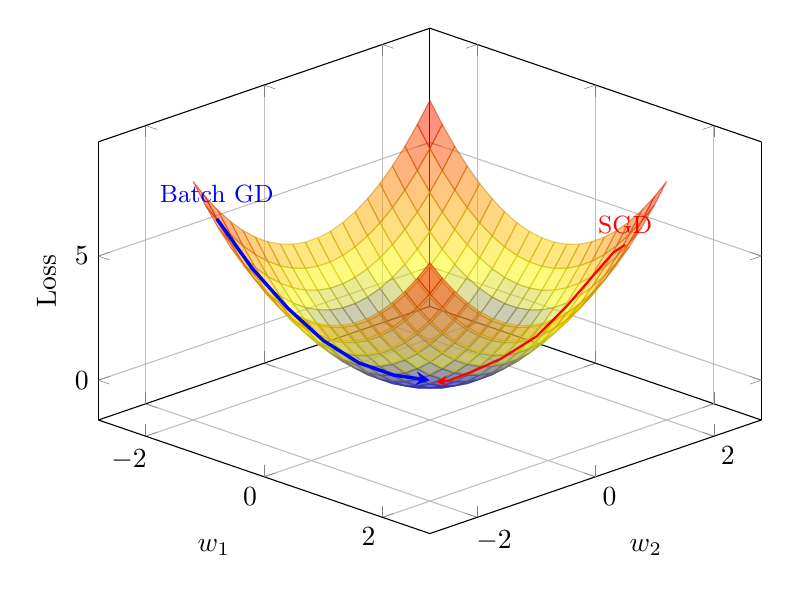
\begin{tikzpicture}[scale=1.0]
    \begin{axis}[
        view={45}{30},
        xlabel={$w_1$},
        ylabel={$w_2$},
        zlabel={Loss},
        width=10cm,
        height=8cm,
        grid=major,
        enlargelimits=0.2  
    ]
% Loss surface (simplified)
    \addplot3[
        surf,
        domain=-2:2,
        domain y=-2:2,
        samples=20,
        opacity=0.5
    ] {x^2 + y^2};
% Batch GD path (smooth)
    \addplot3[blue, very thick, -stealth] coordinates {
        (-1.8, -1.8, 6.5) (-1.5, -1.5, 4.5) (-1.2, -1.2, 2.9)
        (-0.9, -0.9, 1.6) (-0.6, -0.6, 0.7) (-0.3, -0.3, 0.2) (0, 0, 0)
    };
    \node[blue, font=\small] at (axis cs:-1.8,-1.8,7.5) {Batch GD};
% SGD path (noisy)
    \addplot3[red, thick, -stealth] coordinates {
        (1.8, 1.5, 5.7) (1.4, 1.7, 4.9) (1.0, 1.3, 2.7)
        (0.8, 1.0, 1.6) (0.5, 0.7, 0.7) (0.3, 0.4, 0.25)
        (0.2, 0.1, 0.05) (0.1, 0, 0.01)
    };
    \node[red, font=\small] at (axis cs:1.8,1.5,6.5) {SGD};
    \end{axis}
\end{tikzpicture}
\end{center}

\textbf{Batch GD:} Smooth path directly to minimum

\textbf{SGD:} Noisy, bouncing path that eventually converges
\end{geometrybox}

\subsection{Learning Rate Selection}

\begin{importantbox}
\textbf{Choosing Learning Rate $\alpha$:}

\textbf{Too small ($\alpha = 0.0001$):}
\begin{itemize}
    \item Very slow learning
    \item May take forever to converge
    \item Safe but inefficient
\end{itemize}

\textbf{Too large ($\alpha = 10$):}
\begin{itemize}
    \item Overshoots minimum
    \item Loss may increase or oscillate
    \item May diverge completely!
\end{itemize}

\textbf{Just right ($\alpha = 0.01$ or $0.001$):}
\begin{itemize}
    \item Steady decrease in loss
    \item Reasonable convergence speed
\end{itemize}

\textbf{Best practice:}
\begin{itemize}
    \item Start with $\alpha = 0.01$ or $0.001$
    \item Use learning rate schedules (decrease over time)
    \item Try: $0.1, 0.01, 0.001, 0.0001$ and see which works best
    \item Use adaptive methods (Adam, RMSprop) that adjust $\alpha$ automatically
\end{itemize}
\end{importantbox}

\section{Universal Approximation Theorem}

\begin{theorem}[Universal Approximation Theorem]
A feed-forward neural network with:
\begin{itemize}
    \item A single hidden layer
    \item Finite number of neurons
    \item Non-linear activation function
\end{itemize}

can approximate any continuous function on a compact subset of $\mathbb{R}^n$ to arbitrary accuracy.

\textbf{In simple terms:} Neural networks can learn ANY function, given enough neurons!

\textbf{Caveat:} The theorem guarantees existence, not:
\begin{itemize}
    \item How to find the weights (training may be hard)
    \item How many neurons are needed (may need many!)
    \item Whether it will generalize well
\end{itemize}
\end{theorem}

\begin{mentalmodel}
\textbf{Why is this powerful?}

You don't need to manually engineer features or specify the functional form.

Just give the network enough capacity (neurons), and it will learn the right representation from data!

\textbf{This is why deep learning is so successful!}
\end{mentalmodel}

\section{Preventing Overfitting in Neural Networks}

\subsection{Regularization Techniques}

\begin{definition}[L2 Regularization (Weight Decay)]
Add penalty term to loss:
\begin{equation}
    L_{\text{regularized}} = L + \frac{\lambda}{2}\sum_{\ell}\sum_{i,j}(W_{ij}^{[\ell]})^2
\end{equation}

\textbf{Effect:} Encourages smaller weights → simpler model → less overfitting

\textbf{Update rule:}
\begin{equation}
    \mathbf{W}^{[\ell]} \leftarrow (1 - \alpha\lambda)\mathbf{W}^{[\ell]} - \alpha\frac{\partial L}{\partial \mathbf{W}^{[\ell]}}
\end{equation}

The term $(1 - \alpha\lambda)$ shrinks weights slightly each iteration (hence "weight decay").
\end{definition}

\begin{definition}[Dropout]
During training, randomly "drop" (set to 0) neurons with probability $p$ (typically 0.5).

\textbf{Algorithm (training):}
\begin{enumerate}
    \item For each mini-batch:
    \begin{enumerate}
        \item For each layer, randomly select $p$ fraction of neurons
        \item Set their activations to 0
        \item Forward and backward pass with remaining neurons
    \end{enumerate}
\end{enumerate}

\textbf{At test time:} Use all neurons but scale activations by $(1-p)$

\textbf{Effect:}
\begin{itemize}
    \item Prevents co-adaptation of neurons
    \item Forces network to learn robust features
    \item Similar to training an ensemble of many networks
\end{itemize}

\textbf{Extremely effective in practice!}
\end{definition}

\begin{definition}[Early Stopping]
\textbf{Algorithm:}
\begin{enumerate}
    \item Split data: Training + Validation
    \item Train network, monitoring validation loss
    \item When validation loss stops decreasing (or starts increasing):
    \begin{itemize}
        \item Stop training
        \item Restore weights from best validation epoch
    \end{itemize}
\end{enumerate}

\textbf{Simple but very effective!}
\end{definition}

\section{Practical Considerations}

\subsection{Weight Initialization}

\begin{importantbox}
\textbf{Why initialization matters:}

\textbf{All zeros:}
\begin{itemize}
    \item All neurons compute same function
    \item Gradients are identical
    \item Network can't break symmetry
    \item \textbf{Never use!}
\end{itemize}

\textbf{Too large:}
\begin{itemize}
    \item Activations saturate (sigmoid/tanh)
    \item Gradients vanish
    \item Learning is very slow
\end{itemize}

\textbf{Good initialization (Xavier/He):}

\textbf{Xavier (Glorot) initialization (for sigmoid/tanh):}
\begin{equation}
    W_{ij} \sim \mathcal{N}\left(0, \frac{2}{n_{\text{in}} + n_{\text{out}}}\right)
\end{equation}

\textbf{He initialization (for ReLU):}
\begin{equation}
    W_{ij} \sim \mathcal{N}\left(0, \frac{2}{n_{\text{in}}}\right)
\end{equation}

where $n_{\text{in}}$ is number of input neurons, $n_{\text{out}}$ is number of output neurons.

\textbf{Effect:} Keeps variance of activations and gradients stable across layers.
\end{importantbox}

\subsection{Batch Normalization}

\begin{definition}[Batch Normalization]
Normalize activations within each mini-batch:

For each layer, compute:
\begin{align}
    \mu_B &= \frac{1}{m}\sum_{i=1}^{m} z_i \\
    \sigma_B^2 &= \frac{1}{m}\sum_{i=1}^{m}(z_i - \mu_B)^2 \\
    \hat{z}_i &= \frac{z_i - \mu_B}{\sqrt{\sigma_B^2 + \epsilon}}
\end{align}

Then apply learnable scale and shift:
\begin{equation}
    \tilde{z}_i = \gamma \hat{z}_i + \beta
\end{equation}

\textbf{Benefits:}
\begin{itemize}
    \item Reduces internal covariate shift
    \item Allows higher learning rates
    \item Reduces sensitivity to initialization
    \item Acts as regularizer
    \item Accelerates training significantly
\end{itemize}

\textbf{Very popular in modern deep networks!}
\end{definition}

\section{Advantages and Disadvantages}

\begin{keyidea}
\textbf{Advantages:}

\begin{enumerate}
    \item \textbf{Universal approximator:} Can learn any function
    \item \textbf{Automatic feature learning:} No manual feature engineering
    \item \textbf{Non-linear:} Captures complex patterns
    \item \textbf{Flexible:} Works for regression, classification, etc.
    \item \textbf{Powerful:} State-of-the-art for many tasks
    \item \textbf{Scalable:} Benefits from more data and compute
    \item \textbf{Transfer learning:} Can reuse learned features
\end{enumerate}

\textbf{Disadvantages:}

\begin{enumerate}
    \item \textbf{Black box:} Hard to interpret
    \item \textbf{Data hungry:} Needs lots of training data
    \item \textbf{Computationally expensive:} Training can take days/weeks
    \item \textbf{Many hyperparameters:} Architecture, learning rate, regularization, etc.
    \item \textbf{Overfitting prone:} Especially with small data
    \item \textbf{Local minima:} Optimization not guaranteed to find global optimum
    \item \textbf{Unstable:} Small changes in data/hyperparameters can give very different results
    \item \textbf{Requires expertise:} Hard to get working well
\end{enumerate}
\end{keyidea}

\section{GATE-Style Problems}

\begin{example}[Problem 1: Counting Parameters]

\textbf{Question:} A neural network has:
\begin{itemize}
    \item Input: 10 features
    \item Hidden layer 1: 20 neurons
    \item Hidden layer 2: 15 neurons
    \item Output: 3 neurons
\end{itemize}

How many total parameters (weights + biases)?

\textbf{Solution:}

\textbf{Layer 1:} Input (10) → Hidden 1 (20)
\begin{itemize}
    \item Weights: $10 \times 20 = 200$
    \item Biases: $20$
    \item Total: $220$
\end{itemize}

\textbf{Layer 2:} Hidden 1 (20) → Hidden 2 (15)
\begin{itemize}
    \item Weights: $20 \times 15 = 300$
    \item Biases: $15$
    \item Total: $315$
\end{itemize}

\textbf{Layer 3:} Hidden 2 (15) → Output (3)
\begin{itemize}
    \item Weights: $15 \times 3 = 45$
    \item Biases: $3$
    \item Total: $48$
\end{itemize}

\textbf{Total parameters:} $220 + 315 + 48 = 583$
\end{example}

\begin{example}[Problem 2: Activation Functions]

\textbf{Question:} Which activation function should be used for:
\begin{enumerate}
    \item Binary classification output layer?
    \item Multi-class classification output layer?
    \item Hidden layers in deep network?
    \item Regression output (positive values only)?
\end{enumerate}

\textbf{Answer:}

\begin{enumerate}
    \item \textbf{Sigmoid} - outputs probability in (0,1)
    \item \textbf{Softmax} - outputs probability distribution over classes
    \item \textbf{ReLU} - prevents vanishing gradients, fast to compute
    \item \textbf{ReLU or Linear} - ReLU ensures non-negative, Linear for any range
\end{enumerate}
\end{example}

\begin{example}[Problem 3: Forward Propagation]

\textbf{Given:}
\begin{itemize}
    \item Input: $\mathbf{x} = [2, 3]^T$
    \item Weights: $\mathbf{W} = \begin{bmatrix} 1 & 0 \\ 0 & 1 \end{bmatrix}$
    \item Bias: $\mathbf{b} = [1, -1]^T$
    \item Activation: ReLU
\end{itemize}

\textbf{Compute output.}

\textbf{Solution:}

\textbf{Pre-activation:}
\begin{align}
    \mathbf{z} &= \mathbf{W}\mathbf{x} + \mathbf{b} \\
    &= \begin{bmatrix} 1 & 0 \\ 0 & 1 \end{bmatrix}\begin{bmatrix} 2 \\ 3 \end{bmatrix} + \begin{bmatrix} 1 \\ -1 \end{bmatrix} \\
    &= \begin{bmatrix} 2 \\ 3 \end{bmatrix} + \begin{bmatrix} 1 \\ -1 \end{bmatrix} \\
    &= \begin{bmatrix} 3 \\ 2 \end{bmatrix}
\end{align}

\textbf{Activation:}
\begin{align}
    \mathbf{a} &= \text{ReLU}(\mathbf{z}) \\
    &= \begin{bmatrix} \max(0, 3) \\ \max(0, 2) \end{bmatrix} \\
    &= \begin{bmatrix} 3 \\ 2 \end{bmatrix}
\end{align}
\end{example}

\begin{example}[Problem 4: Learning Rate Effect]
\mbox{}\\
\textbf{Question:} What happens if learning rate is:
\begin{enumerate}
    \item Too large?
    \item Too small?
\end{enumerate}

\textbf{Answer:}

\begin{enumerate}
    \item \textbf{Too large:}
    \begin{itemize}
        \item Updates overshoot minimum
        \item Loss oscillates or increases
        \item May diverge completely
        \item Training unstable
    \end{itemize}
    
    \item \textbf{Too small:}
    \begin{itemize}
        \item Very slow learning
        \item May get stuck in local minimum
        \item Takes very long to converge
        \item Training inefficient but stable
    \end{itemize}
\end{enumerate}
\end{example}

\section{Summary - Key Points for GATE}

\begin{importantbox}
\textbf{Must Know for GATE:}

\begin{enumerate}
    \item \textbf{Architecture:}
    \begin{itemize}
        \item Input layer → Hidden layer(s) → Output layer
        \item Fully connected (each neuron connects to all in next layer)
        \item Feed-forward (no cycles)
    \end{itemize}
    
    \item \textbf{Neuron computation:}
    \begin{equation}
        z = \mathbf{w}^T\mathbf{x} + b, \quad a = \sigma(z)
    \end{equation}
    
    \item \textbf{Activation functions:}
    \begin{itemize}
        \item Sigmoid: $\frac{1}{1+e^{-z}}$, range (0,1)
        \item Tanh: $\frac{e^z - e^{-z}}{e^z + e^{-z}}$, range (-1,1)
        \item ReLU: $\max(0, z)$, range $[0, \infty)$
        \item Softmax: $\frac{e^{z_k}}{\sum_j e^{z_j}}$ for multi-class
    \end{itemize}
    
    \item \textbf{Forward propagation:}
    \begin{align}
        \mathbf{z}^{[\ell]} &= \mathbf{W}^{[\ell]}\mathbf{a}^{[\ell-1]} + \mathbf{b}^{[\ell]} \\
        \mathbf{a}^{[\ell]} &= \sigma(\mathbf{z}^{[\ell]})
    \end{align}
    
    \item \textbf{Backpropagation:}
    \begin{itemize}
        \item Efficiently computes gradients using chain rule
        \item Propagates error backward from output to input
        \item Complexity: $O(\text{forward pass})$
    \end{itemize}
    
    \item \textbf{Training:}
    \begin{itemize}
        \item Gradient descent: $\mathbf{W} \leftarrow \mathbf{W} - \alpha \frac{\partial L}{\partial \mathbf{W}}$
        \item Batch GD: Use all data
        \item Mini-batch: Use small batches (most common)
        \item SGD: Use one sample at a time
    \end{itemize}
    
    \item \textbf{Loss functions:}
    \begin{itemize}
        \item MSE for regression
        \item Cross-entropy for classification
    \end{itemize}
    
    \item \textbf{Regularization:}
    \begin{itemize}
        \item L2 (weight decay)
        \item Dropout
        \item Early stopping
    \end{itemize}
    
    \item \textbf{Universal Approximation:} Single hidden layer can approximate any continuous function
    
    \item \textbf{Parameter count:}
    \begin{equation}
        \text{Params} = \sum_{\ell}(n_{\ell-1} \times n_{\ell} + n_{\ell})
    \end{equation}
    
    \item \textbf{Key challenges:}
    \begin{itemize}
        \item Vanishing/exploding gradients
        \item Overfitting
        \item Local minima
        \item Hyperparameter tuning
    \end{itemize}
\end{enumerate}
\end{importantbox}

\begin{gatepoint}
\textbf{Common GATE Question Types:}

\begin{enumerate}
    \item Count total parameters in a network
    \item Compute forward pass by hand
    \item Choose appropriate activation functions
    \item Understand gradient descent variants
    \item Explain backpropagation concept
    \item Know when to use which loss function
    \item Understand vanishing gradient problem
    \item Compare with other ML algorithms
    \item Explain regularization techniques
    \item Understand Universal Approximation Theorem
    \item Know effects of hyperparameters (learning rate, architecture)
    \item Identify overfitting/underfitting
\end{enumerate}
\end{gatepoint}
\chapter{Clustering: K-means, K-medoid, and Hierarchical Methods}

\section{Introduction to Clustering}

\begin{mentalmodel}
Imagine organizing a messy closet:

\textbf{You don't have labels like "shirts," "pants," "shoes"}

Instead, you:
\begin{enumerate}
    \item Look at items and notice similarities
    \item Group similar items together
    \item Create piles: "long items," "small items," "footwear," etc.
    \item You've discovered natural groupings without being told what they are!
\end{enumerate}

\textbf{This is exactly what clustering does with data!}

It finds natural groups in unlabeled data.
\end{mentalmodel}

\begin{keyidea}
\textbf{Clustering} is an \textbf{unsupervised learning} technique that groups similar data points together.

\textbf{Key differences from classification:}
\begin{itemize}
    \item \textbf{Unsupervised:} No labels provided
    \item \textbf{Discovery:} Find hidden structure in data
    \item \textbf{Exploratory:} Often used to understand data
\end{itemize}

\textbf{Goals:}
\begin{enumerate}
    \item High \textbf{intra-cluster similarity:} Points within a cluster are similar
    \item Low \textbf{inter-cluster similarity:} Points in different clusters are dissimilar
\end{enumerate}

\textbf{Applications:}
\begin{itemize}
    \item Customer segmentation (marketing)
    \item Image segmentation (computer vision)
    \item Document clustering (information retrieval)
    \item Gene expression analysis (bioinformatics)
    \item Anomaly detection
\end{itemize}
\end{keyidea}

\section{Distance Metrics}

\begin{definition}[Distance Measures]
Clustering requires a measure of similarity/dissimilarity between points.

\textbf{1. Euclidean Distance:}
\begin{equation}
    d(\mathbf{x}, \mathbf{y}) = \sqrt{\sum_{i=1}^{p}(x_i - y_i)^2} = ||\mathbf{x} - \mathbf{y}||_2
\end{equation}

Most common; assumes all features equally important.

\textbf{2. Manhattan Distance (L1):}
\begin{equation}
    d(\mathbf{x}, \mathbf{y}) = \sum_{i=1}^{p}|x_i - y_i|
\end{equation}

Less sensitive to outliers than Euclidean.

\textbf{3. Cosine Similarity:}
\begin{equation}
    \text{similarity}(\mathbf{x}, \mathbf{y}) = \frac{\mathbf{x}^T\mathbf{y}}{||\mathbf{x}|| \cdot ||\mathbf{y}||} = \cos(\theta)
\end{equation}

Measures angle between vectors; useful for text data.

\textbf{Cosine distance:}
\begin{equation}
    d(\mathbf{x}, \mathbf{y}) = 1 - \text{similarity}(\mathbf{x}, \mathbf{y})
\end{equation}

\textbf{4. Minkowski Distance:}
\begin{equation}
    d(\mathbf{x}, \mathbf{y}) = \left(\sum_{i=1}^{p}|x_i - y_i|^q\right)^{1/q}
\end{equation}

Generalizes Euclidean ($q=2$) and Manhattan ($q=1$).
\end{definition}

\section{K-means Clustering}

\subsection{Algorithm}

\begin{definition}[K-means Algorithm]
\textbf{Goal:} Partition $n$ data points into $k$ clusters by minimizing within-cluster variance.

\textbf{Input:}
\begin{itemize}
    \item Data: $\{\mathbf{x}_1, \mathbf{x}_2, \ldots, \mathbf{x}_n\}$
    \item Number of clusters: $k$
\end{itemize}

\textbf{Output:}
\begin{itemize}
    \item Cluster assignments: $\{C_1, C_2, \ldots, C_k\}$
    \item Cluster centers (centroids): $\{\boldsymbol{\mu}_1, \boldsymbol{\mu}_2, \ldots, \boldsymbol{\mu}_k\}$
\end{itemize}

\textbf{Algorithm:}
\begin{enumerate}
    \item \textbf{Initialize:} Randomly select $k$ points as initial centroids
    
    \item \textbf{Repeat until convergence:}
    \begin{enumerate}
        \item \textbf{Assignment Step:} Assign each point to nearest centroid
        \begin{equation}
            C_j = \{\mathbf{x}_i : ||\mathbf{x}_i - \boldsymbol{\mu}_j||^2 \leq ||\mathbf{x}_i - \boldsymbol{\mu}_\ell||^2 \text{ for all } \ell\}
        \end{equation}
        
        \item \textbf{Update Step:} Recompute centroids as mean of assigned points
        \begin{equation}
            \boldsymbol{\mu}_j = \frac{1}{|C_j|}\sum_{\mathbf{x}_i \in C_j}\mathbf{x}_i
        \end{equation}
    \end{enumerate}
    
    \item \textbf{Convergence:} Stop when centroids don't change (or change very little)
\end{enumerate}
\end{definition}

\begin{geometrybox}
\textbf{K-means Visualization:}

\begin{center}
\resizebox{\linewidth}{!}{%
\begin{tikzpicture}
    % =====================
    % Initial state
    % =====================
    \begin{scope}[shift={(0,0)}]
        % Data points
        \foreach \x/\y in {1/1, 1.5/1.2, 1.2/0.8, 5/5, 5.5/5.2, 5.3/4.8, 2/5, 2.2/5.3, 1.8/4.7} {
            \fill[blue] (\x,\y) circle (2pt);
        }
        % Initial centroids
        \fill[red] (3,2) circle (4pt) node[below right] {$\mu_1$};
        \fill[red] (4,4) circle (4pt) node[below right] {$\mu_2$};
        
        \node at (3, -0.8) {\textbf{Step 0: Initialize}};
        \draw[->] (0,0) -- (6,0);
        \draw[->] (0,0) -- (0,6);
    \end{scope}
    
    % =====================
    % Assignment step
    % =====================
    \begin{scope}[shift={(7.5,0)}]
        \foreach \x/\y in {1/1, 1.5/1.2, 1.2/0.8} {
            \fill[red] (\x,\y) circle (2pt);
        }
        \foreach \x/\y in {5/5, 5.5/5.2, 5.3/4.8, 2/5, 2.2/5.3, 1.8/4.7} {
            \fill[green!70!black] (\x,\y) circle (2pt);
        }
        % Old centroids
        \fill[gray, opacity=0.5] (3,2) circle (4pt);
        \fill[gray, opacity=0.5] (4,4) circle (4pt);
        
        \node at (3, -0.8) {\textbf{Step 1: Assign}};
        \draw[->] (0,0) -- (6,0);
        \draw[->] (0,0) -- (0,6);
    \end{scope}
    
    % =====================
    % Update step
    % =====================
    \begin{scope}[shift={(15,0)}]
        \foreach \x/\y in {1/1, 1.5/1.2, 1.2/0.8} {
            \fill[red] (\x,\y) circle (2pt);
        }
        \foreach \x/\y in {5/5, 5.5/5.2, 5.3/4.8, 2/5, 2.2/5.3, 1.8/4.7} {
            \fill[green!70!black] (\x,\y) circle (2pt);
        }
        % New centroids
        \fill[red] (1.23,1.0) circle (4pt) node[below right] {$\mu_1$};
        \fill[green!70!black] (3.6,5.0) circle (4pt) node[below right] {$\mu_2$};
        
        \node at (3, -0.8) {\textbf{Step 2: Update}};
        \draw[->] (0,0) -- (6,0);
        \draw[->] (0,0) -- (0,6);
    \end{scope}
\end{tikzpicture}
}
\end{center}

Process repeats: assign → update → assign → update... until convergence.
\end{geometrybox}

\subsection{Objective Function}

\begin{definition}[K-means Objective]
K-means minimizes the \textbf{within-cluster sum of squares (WCSS)}:

\begin{equation}
    J = \sum_{j=1}^{k}\sum_{\mathbf{x}_i \in C_j}||\mathbf{x}_i - \boldsymbol{\mu}_j||^2
\end{equation}

Also called \textbf{inertia} or \textbf{distortion}.

\textbf{Properties:}
\begin{itemize}
    \item Each iteration decreases (or maintains) $J$
    \item Algorithm always converges (to a local minimum)
    \item Different initializations → different local minima
\end{itemize}
\end{definition}

\begin{example}[K-means by Hand]

\textbf{Data:} 6 points in 1D: $\{1, 2, 5, 6, 9, 10\}$

\textbf{Goal:} Cluster into $k=2$ groups

\textbf{INITIALIZATION:}

Randomly select: $\mu_1 = 2$, $\mu_2 = 5$

\textbf{ITERATION 1:}

\textbf{Assignment:} Assign each point to nearest centroid
\begin{align}
    \text{Point 1:} & \quad |1-2|=1 < |1-5|=4 \to \text{Cluster 1} \\
    \text{Point 2:} & \quad |2-2|=0 < |2-5|=3 \to \text{Cluster 1} \\
    \text{Point 5:} & \quad |5-2|=3 > |5-5|=0 \to \text{Cluster 2} \\
    \text{Point 6:} & \quad |6-2|=4 > |6-5|=1 \to \text{Cluster 2} \\
    \text{Point 9:} & \quad |9-2|=7 > |9-5|=4 \to \text{Cluster 2} \\
    \text{Point 10:} & \quad |10-2|=8 > |10-5|=5 \to \text{Cluster 2}
\end{align}

\textbf{Clusters:}
\begin{itemize}
    \item $C_1 = \{1, 2\}$
    \item $C_2 = \{5, 6, 9, 10\}$
\end{itemize}

\textbf{Update:} Compute new centroids
\begin{align}
    \mu_1 &= \frac{1 + 2}{2} = 1.5 \\
    \mu_2 &= \frac{5 + 6 + 9 + 10}{4} = 7.5
\end{align}

\textbf{ITERATION 2:}

\textbf{Assignment:} With $\mu_1 = 1.5$, $\mu_2 = 7.5$
\begin{align}
    \text{Point 1:} & \quad |1-1.5|=0.5 < |1-7.5|=6.5 \to \text{Cluster 1} \\
    \text{Point 2:} & \quad |2-1.5|=0.5 < |2-7.5|=5.5 \to \text{Cluster 1} \\
    \text{Point 5:} & \quad |5-1.5|=3.5 < |5-7.5|=2.5 \to \text{Cluster 2} \\
    \text{Point 6:} & \quad |6-1.5|=4.5 < |6-7.5|=1.5 \to \text{Cluster 2} \\
    \text{Point 9:} & \quad |9-1.5|=7.5 > |9-7.5|=1.5 \to \text{Cluster 2} \\
    \text{Point 10:} & \quad |10-1.5|=8.5 > |10-7.5|=2.5 \to \text{Cluster 2}
\end{align}

Wait, point 5 changed! Let's recalculate:
\begin{itemize}
    \item Point 5: $|5-1.5|=3.5$ vs $|5-7.5|=2.5$ → Cluster 2 $checked$
\end{itemize}

\textbf{Clusters:}
\begin{itemize}
    \item $C_1 = \{1, 2\}$
    \item $C_2 = \{5, 6, 9, 10\}$
\end{itemize}

Same as before!

\textbf{Update:}
\begin{align}
    \mu_1 &= 1.5 \\
    \mu_2 &= 7.5
\end{align}

\textbf{Centroids unchanged → CONVERGED!}

\textbf{Final clusters:}
\begin{itemize}
    \item Cluster 1: $\{1, 2\}$ with centroid $1.5$
    \item Cluster 2: $\{5, 6, 9, 10\}$ with centroid $7.5$
\end{itemize}

\textbf{WCSS:}
\begin{align}
    J &= (1-1.5)^2 + (2-1.5)^2 + (5-7.5)^2 + (6-7.5)^2 + (9-7.5)^2 + (10-7.5)^2 \\
    &= 0.25 + 0.25 + 6.25 + 2.25 + 2.25 + 6.25 \\
    &= 17.5
\end{align}
\end{example}

\subsection{Choosing K}

\begin{definition}[Methods to Choose K]

\textbf{1. Elbow Method:}
\begin{itemize}
    \item Plot WCSS vs $k$
    \item Look for "elbow" - point where WCSS decreases sharply then levels off
    \item Choose $k$ at the elbow
\end{itemize}

\textbf{2. Silhouette Score:}

For each point $i$:
\begin{align}
    a(i) &= \text{average distance to points in same cluster} \\
    b(i) &= \text{average distance to points in nearest other cluster} \\
    s(i) &= \frac{b(i) - a(i)}{\max(a(i), b(i))}
\end{align}

$s(i) \in [-1, 1]$:
\begin{itemize}
    \item $s(i) \approx 1$: Well clustered
    \item $s(i) \approx 0$: On border
    \item $s(i) < 0$: Possibly wrong cluster
\end{itemize}

Choose $k$ with highest average silhouette score.

\textbf{3. Domain Knowledge:}
\begin{itemize}
    \item Sometimes $k$ is known from problem context
    \item Example: Customer segments (small, medium, large business)
\end{itemize}
\end{definition}
\pagebreak
\begin{geometrybox}
\textbf{Elbow Method Plot:}

\begin{center}
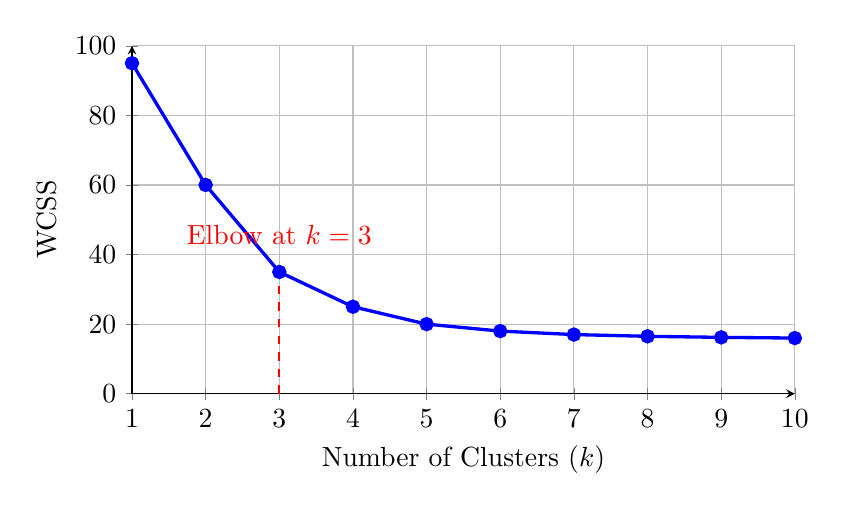
\begin{tikzpicture}[scale=1.0]
    \begin{axis}[
        axis lines = left,
        xlabel = {Number of Clusters ($k$)},
        ylabel = {WCSS},
        xmin=1, xmax=10,
        ymin=0, ymax=100,
        width=10cm,
        height=6cm,
        xtick={1,2,3,4,5,6,7,8,9,10},
        grid=major
    ]
    
    \addplot[blue, very thick, mark=*] coordinates {
        (1, 95) (2, 60) (3, 35) (4, 25) (5, 20) (6, 18) (7, 17) (8, 16.5) (9, 16.2) (10, 16)
    };
    
    % Elbow indicator
    \draw[red, thick, dashed] (3, 0) -- (3, 35);
    \node[red, above] at (3, 40) {Elbow at $k=3$};
    
    \end{axis}
\end{tikzpicture}
\end{center}

Sharp decrease until $k=3$, then levels off → Choose $k=3$
\end{geometrybox}

\subsection{K-means++}

\begin{definition}[K-means++ Initialization]
\textbf{Problem with random initialization:} Can lead to poor local minima.

\textbf{K-means++ solution:} Smart initialization that spreads out initial centroids.

\textbf{Algorithm:}
\begin{enumerate}
    \item Choose first centroid $\mu_1$ uniformly at random from data
    
    \item For $j = 2, 3, \ldots, k$:
    \begin{enumerate}
        \item For each point $\mathbf{x}_i$, compute $D(\mathbf{x}_i)$ = distance to nearest existing centroid
        \item Choose next centroid $\mu_j$ with probability $\propto D(\mathbf{x}_i)^2$
        
        (Points far from existing centroids more likely to be chosen)
    \end{enumerate}
    
    \item Proceed with standard k-means
\end{enumerate}

\textbf{Advantages:}
\begin{itemize}
    \item Faster convergence
    \item Better final clustering (provably)
    \item \textbf{Default in scikit-learn!}
\end{itemize}
\end{definition}

\subsection{Advantages and Disadvantages}

\begin{keyidea}
\textbf{Advantages of K-means:}

\begin{enumerate}
    \item \textbf{Simple:} Easy to understand and implement
    \item \textbf{Fast:} $O(nkdT)$ where $T$ is number of iterations (usually small)
    \item \textbf{Scalable:} Works well with large datasets
    \item \textbf{Guaranteed convergence:} Always converges to local minimum
    \item \textbf{Efficient:} Each iteration is computationally cheap
\end{enumerate}

\textbf{Disadvantages of K-means:}

\begin{enumerate}
    \item \textbf{Must specify $k$:} Number of clusters not learned
    \item \textbf{Sensitive to initialization:} Different starts → different results
    \item \textbf{Assumes spherical clusters:} Fails for elongated or irregular shapes
    \item \textbf{Sensitive to outliers:} Mean is affected by extreme values
    \item \textbf{Assumes equal variance:} All clusters have similar spread
    \item \textbf{Hard assignment:} Each point belongs to exactly one cluster
    \item \textbf{Local minima:} May not find global optimum
\end{enumerate}
\end{keyidea}

\section{K-medoid Clustering (PAM)}

\subsection{Motivation}

\begin{mentalmodel}
\textbf{Problem with K-means:}

The centroid $\boldsymbol{\mu} = \frac{1}{n}\sum \mathbf{x}_i$ might not be an actual data point!

\textbf{Example:} Clustering cities by location
\begin{itemize}
    \item Centroid might be in the ocean or desert (not a real city)
    \item Would be better to choose an actual city as representative
\end{itemize}

\textbf{K-medoid solution:} Use actual data points as cluster centers (medoids)!
\end{mentalmodel}

\begin{definition}[Medoid]
A \textbf{medoid} is the most centrally located point in a cluster.

\textbf{Formal definition:} Point that minimizes sum of distances to all other points in cluster:

\begin{equation}
    \text{medoid} = \arg\min_{\mathbf{x}_i \in C} \sum_{\mathbf{x}_j \in C} d(\mathbf{x}_i, \mathbf{x}_j)
\end{equation}

\textbf{Key difference from mean:} Medoid must be an actual data point.
\end{definition}

\subsection{PAM Algorithm}

\begin{definition}[Partitioning Around Medoids (PAM)]
\textbf{Goal:} Partition data into $k$ clusters using medoids.

\textbf{Algorithm:}

\textbf{Phase 1: BUILD}
\begin{enumerate}
    \item Select $k$ initial medoids (similar to k-means++)
\end{enumerate}

\textbf{Phase 2: SWAP}
\begin{enumerate}
    \item Assign each point to nearest medoid
    
    \item For each medoid $m$ and each non-medoid point $p$:
    \begin{enumerate}
        \item Swap $m$ and $p$ (tentatively)
        \item Compute total cost (sum of distances from all points to nearest medoid)
        \item If cost decreases: Make swap permanent
    \end{enumerate}
    
    \item Repeat until no beneficial swaps remain
\end{enumerate}

\textbf{Cost function:}
\begin{equation}
    J = \sum_{j=1}^{k}\sum_{\mathbf{x}_i \in C_j} d(\mathbf{x}_i, m_j)
\end{equation}

where $m_j$ is the medoid of cluster $j$.
\end{definition}

\begin{example}[K-medoid vs K-means]

\textbf{Data:} $\{1, 2, 3, 100\}$ in 1D, $k=1$

\textbf{K-means:}
\begin{align}
    \text{Centroid} &= \frac{1 + 2 + 3 + 100}{4} = 26.5
\end{align}

Not a data point! Pulled by outlier (100).

\textbf{K-medoid:}

Try each point as medoid:
\begin{align}
    \text{Cost}(1) &= |1-1| + |2-1| + |3-1| + |100-1| = 0 + 1 + 2 + 99 = 102 \\
    \text{Cost}(2) &= |1-2| + |2-2| + |3-2| + |100-2| = 1 + 0 + 1 + 98 = 100 \\
    \text{Cost}(3) &= |1-3| + |2-3| + |3-3| + |100-3| = 2 + 1 + 0 + 97 = 100 \\
    \text{Cost}(100) &= |1-100| + |2-100| + |3-100| + |100-100| = 99 + 98 + 97 + 0 = 294
\end{align}

\textbf{Medoid:} Point 2 or 3 (cost = 100)

More robust to outlier!
\end{example}

\subsection{Advantages and Disadvantages}

\begin{importantbox}
\textbf{Advantages of K-medoid:}

\begin{enumerate}
    \item \textbf{Robust to outliers:} Medoid not affected by extreme values
    \item \textbf{Interpretable:} Representative is actual data point
    \item \textbf{Any distance metric:} Works with any dissimilarity measure
    \item \textbf{Meaningful centers:} Cluster representative makes sense
\end{enumerate}

\textbf{Disadvantages of K-medoid:}

\begin{enumerate}
    \item \textbf{Computationally expensive:} $O(k(n-k)^2)$ per iteration
    \item \textbf{Slower than K-means:} Especially for large datasets
    \item \textbf{Still needs $k$:} Number of clusters must be specified
    \item \textbf{Local minima:} Same problem as K-means
\end{enumerate}

\textbf{When to use K-medoid over K-means:}
\begin{itemize}
    \item Data contains outliers
    \item Need interpretable cluster centers
    \item Using non-Euclidean distance metric
    \item Dataset is small enough (computational cost acceptable)
\end{itemize}
\end{importantbox}

\section{Hierarchical Clustering}

\subsection{Overview}

\begin{definition}[Hierarchical Clustering]
\textbf{Hierarchical clustering} builds a tree-like structure (dendrogram) of nested clusters.

\textbf{Two approaches:}

\textbf{1. Agglomerative (Bottom-up):}
\begin{itemize}
    \item Start: Each point is its own cluster
    \item Repeatedly merge closest clusters
    \item End: All points in one cluster
    \item \textbf{Most common!}
\end{itemize}

\textbf{2. Divisive (Top-down):}
\begin{itemize}
    \item Start: All points in one cluster
    \item Repeatedly split clusters
    \item End: Each point is its own cluster
    \item \textbf{Rarely used in practice}
\end{itemize}

\textbf{Output:} Dendrogram showing hierarchy of clusters at different scales.

\textbf{Key advantage:} Don't need to specify $k$ in advance!
\end{definition}

\begin{geometrybox}
\textbf{Dendrogram Example:}

\begin{center}
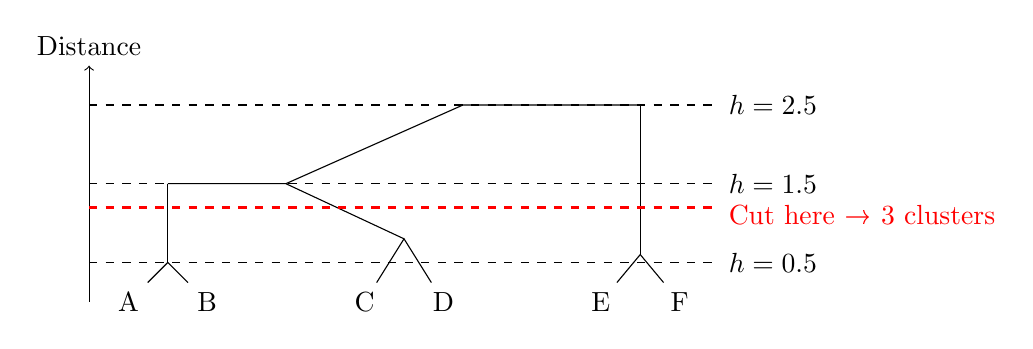
\begin{tikzpicture}[scale=1.0]
    % Leaves (data points)
    \node (a) at (0, 0) {A};
    \node (b) at (1, 0) {B};
    \node (c) at (3, 0) {C};
    \node (d) at (4, 0) {D};
    \node (e) at (6, 0) {E};
    \node (f) at (7, 0) {F};
    
    % First level merges
    \draw (a) -- (0.5, 0.5) -- (b);
    \draw (c) -- (3.5, 0.8) -- (d);
    \draw (e) -- (6.5, 0.6) -- (f);
    
    % Second level
    \draw (0.5, 0.5) -- (0.5, 1.5);
    \draw (3.5, 0.8) -- (2, 1.5) -- (0.5, 1.5);
    
    % Third level
    \draw (6.5, 0.6) -- (6.5, 2.5);
    \draw (2, 1.5) -- (4.25, 2.5) -- (6.5, 2.5);
    
    % Height labels
    \draw[dashed] (-0.5, 0.5) -- (7.5, 0.5) node[right] {$h=0.5$};
    \draw[dashed] (-0.5, 1.5) -- (7.5, 1.5) node[right] {$h=1.5$};
    \draw[dashed] (-0.5, 2.5) -- (7.5, 2.5) node[right] {$h=2.5$};
    
    % Axis
    \draw[->] (-0.5, 0) -- (-0.5, 3) node[above] {Distance};
    
    % Cut line
    \draw[red, very thick, dashed] (-0.5, 1.2) -- (7.5, 1.2);
    \node[red, right] at (7.5, 1.1) {Cut here → 3 clusters};
    
\end{tikzpicture}
\end{center}

\textbf{Reading the dendrogram:}
\begin{itemize}
    \item Height of merge indicates distance between clusters
    \item Cut at different heights → different number of clusters
    \item Cutting at red line gives 3 clusters: \{A,B,C,D\}, \{E,F\}
\end{itemize}
\end{geometrybox}

\subsection{Agglomerative Clustering Algorithm}

\begin{definition}[Agglomerative Hierarchical Clustering]

\textbf{Algorithm:}
\begin{enumerate}
    \item \textbf{Initialize:} Each point is its own cluster
    
    \item \textbf{Compute:} Distance between all pairs of clusters (using linkage criterion)
    
    \item \textbf{Repeat} until one cluster remains:
    \begin{enumerate}
        \item Find two closest clusters
        \item Merge them into one cluster
        \item Update distance matrix
    \end{enumerate}
    
    \item \textbf{Output:} Dendrogram
\end{enumerate}

\textbf{To get $k$ clusters:} Cut dendrogram at appropriate height.
\end{definition}

\subsection{Linkage Criteria}

\begin{definition}[Cluster Distance Measures]

How do we measure distance between two clusters $A$ and $B$?

\textbf{1. Single Linkage (Nearest Neighbor):}
\begin{equation}
    d(A, B) = \min_{\mathbf{x}_i \in A, \mathbf{x}_j \in B} d(\mathbf{x}_i, \mathbf{x}_j)
\end{equation}

Distance between \textbf{closest} points.

\textbf{Properties:}
\begin{itemize}
    \item \textbf{Pros:} Can handle non-elliptical shapes, finds elongated clusters
    \item \textbf{Cons:} Sensitive to noise/outliers, "chaining" effect
\end{itemize}

\textbf{2. Complete Linkage (Farthest Neighbor):}
\begin{equation}
    d(A, B) = \max_{\mathbf{x}_i \in A, \mathbf{x}_j \in B} d(\mathbf{x}_i, \mathbf{x}_j)
\end{equation}

Distance between \textbf{farthest} points.

\textbf{Properties:}
\begin{itemize}
    \item \textbf{Pros:} Compact, spherical clusters; less sensitive to outliers
    \item \textbf{Cons:} Can break large clusters; biased towards equal-sized clusters
\end{itemize}

\textbf{3. Average Linkage:}
\begin{equation}
    d(A, B) = \frac{1}{|A| \cdot |B|}\sum_{\mathbf{x}_i \in A}\sum_{\mathbf{x}_j \in B} d(\mathbf{x}_i, \mathbf{x}_j)
\end{equation}

\textbf{Average} of all pairwise distances.

\textbf{Properties:}
\begin{itemize}
    \item \textbf{Pros:} Balance between single and complete; robust
    \item \textbf{Cons:} More computationally expensive
    \item \textbf{Often best choice in practice!}
\end{itemize}

\textbf{4. Ward's Method:}

Merge clusters that minimize increase in total within-cluster variance:
\begin{equation}
    d(A, B) = \frac{|A| \cdot |B|}{|A| + |B|} ||\boldsymbol{\mu}_A - \boldsymbol{\mu}_B||^2
\end{equation}

\textbf{Properties:}
\begin{itemize}
    \item \textbf{Pros:} Minimizes variance (like K-means objective); compact clusters
    \item \textbf{Cons:} Biased towards equal-sized, spherical clusters
    \item \textbf{Very popular!}
\end{itemize}
\end{definition}

\begin{example}[Linkage Comparison]

\textbf{Two clusters:}
\begin{itemize}
    \item $A = \{1, 2, 3\}$
    \item $B = \{8, 9, 10\}$
\end{itemize}

\textbf{Single linkage:}
\begin{equation}
    d(A, B) = \min\{|1-8|, |1-9|, |1-10|, |2-8|, \ldots, |3-10|\} = |3-8| = 5
\end{equation}

\textbf{Complete linkage:}
\begin{equation}
    d(A, B) = \max\{|1-8|, |1-9|, |1-10|, |2-8|, \ldots, |3-10|\} = |1-10| = 9
\end{equation}

\textbf{Average linkage:}
\begin{align}
    d(A, B) &= \frac{1}{3 \times 3}\sum \text{all pairwise distances} \\
    &= \frac{1}{9}(7 + 8 + 9 + 6 + 7 + 8 + 5 + 6 + 7) \\
    &= \frac{63}{9} = 7
\end{align}
\end{example}

\begin{geometrybox}
\textbf{Linkage Effects:}

\begin{center}
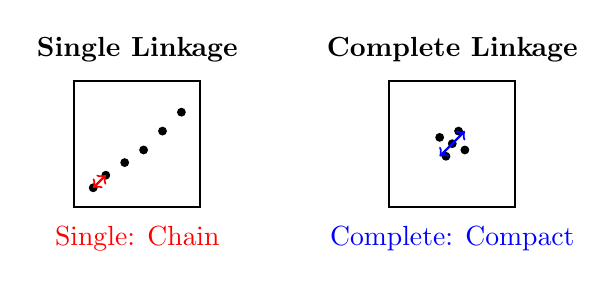
\begin{tikzpicture}[scale=0.8]
    % Single linkage - chaining
    \begin{scope}[shift={(0,0)}]
        \draw[thick] (0,0) rectangle (2,2);
        \fill (0.3,0.3) circle (2pt);
        \fill (0.5,0.5) circle (2pt);
        \fill (0.8,0.7) circle (2pt);
        \fill (1.1,0.9) circle (2pt);
        \fill (1.4,1.2) circle (2pt);
        \fill (1.7,1.5) circle (2pt);
        
        \draw[red, thick, <->] (0.3,0.3) -- (0.5,0.5);
        \node[red] at (1, -0.5) {Single: Chain};
        \node at (1, 2.5) {\textbf{Single Linkage}};
    \end{scope}
    
    % Complete linkage - compact
    \begin{scope}[shift={(5,0)}]
        \draw[thick] (0,0) rectangle (2,2);
        % Compact cluster
        \fill (1,1) circle (2pt);
        \fill (0.8,1.1) circle (2pt);
        \fill (1.2,0.9) circle (2pt);
        \fill (0.9,0.8) circle (2pt);
        \fill (1.1,1.2) circle (2pt);
        
        \draw[blue, thick, <->] (0.8,0.8) -- (1.2,1.2);
        \node[blue] at (1, -0.5) {Complete: Compact};
        \node at (1, 2.5) {\textbf{Complete Linkage}};
    \end{scope}
\end{tikzpicture}
\end{center}
\end{geometrybox}

\subsection{Complete Example}

\begin{example}[Hierarchical Clustering by Hand]

\textbf{Data:} 4 points in 1D: $A=1, B=2, C=5, D=6$

\textbf{Method:} Complete linkage

\textbf{STEP 1: Initial distance matrix}

\begin{center}
\begin{tabular}{|c|c|c|c|c|}
\hline
 & A & B & C & D \\
\hline
A & 0 & 1 & 4 & 5 \\
B & 1 & 0 & 3 & 4 \\
C & 4 & 3 & 0 & 1 \\
D & 5 & 4 & 1 & 0 \\
\hline
\end{tabular}
\end{center}

\textbf{STEP 2: First merge}

Minimum distance: $d(A,B) = 1$ and $d(C,D) = 1$

Merge $A$ and $B$ into cluster $AB$:

\textbf{Update distances (complete linkage):}
\begin{align}
    d(AB, C) &= \max(d(A,C), d(B,C)) = \max(4, 3) = 4 \\
    d(AB, D) &= \max(d(A,D), d(B,D)) = \max(5, 4) = 5
\end{align}

\textbf{New matrix:}
\begin{center}
\begin{tabular}{|c|c|c|c|}
\hline
 & AB & C & D \\
\hline
AB & 0 & 4 & 5 \\
C & 4 & 0 & 1 \\
D & 5 & 1 & 0 \\
\hline
\end{tabular}
\end{center}

\textbf{STEP 3: Second merge}

Minimum distance: $d(C,D) = 1$

Merge $C$ and $D$ into cluster $CD$:

\textbf{Update:}
\begin{equation}
    d(AB, CD) = \max(d(AB,C), d(AB,D)) = \max(4, 5) = 5
\end{equation}

\textbf{STEP 4: Final merge}

Merge $AB$ and $CD$ at distance $5$

\textbf{Dendrogram:}

\begin{center}
\begin{tikzpicture}[scale=1.2]
    % Points
    \node (a) at (0,0) {A};
    \node (b) at (1,0) {B};
    \node (c) at (3,0) {C};
    \node (d) at (4,0) {D};
    
    % First merges at height 1
    \draw (a) -- (0.5, 1) -- (b);
    \draw (c) -- (3.5, 1) -- (d);
    
    % Second merge at height 5
    \draw (0.5, 1) -- (0.5, 5);
    \draw (3.5, 1) -- (3.5, 5);
    \draw (0.5, 5) -- (3.5, 5);
    
    % Height axis
    \draw[->] (-0.5, 0) -- (-0.5, 6) node[above] {Distance};
    \draw (-0.7, 1) -- (-0.5, 1) node[left, xshift=-2mm] {1};
    \draw (-0.7, 5) -- (-0.5, 5) node[left, xshift=-2mm] {5};
\end{tikzpicture}
\end{center}

\textbf{Getting clusters:}
\begin{itemize}
    \item Cut at $h=3$: 2 clusters → $\{A,B\}$, $\{C,D\}$
    \item Cut at $h=0.5$: 4 clusters → $\{A\}$, $\{B\}$, $\{C\}$, $\{D\}$
\end{itemize}
\end{example}

\subsection{Advantages and Disadvantages}

\begin{keyidea}
\textbf{Advantages of Hierarchical Clustering:}

\begin{enumerate}
    \item \textbf{No need to specify $k$:} Can choose number of clusters after seeing dendrogram
    \item \textbf{Hierarchy is informative:} Shows relationships at multiple scales
    \item \textbf{Deterministic:} No random initialization (for same linkage)
    \item \textbf{Visualizable:} Dendrogram is intuitive
    \item \textbf{Flexible:} Various linkage criteria for different needs
    \item \textbf{Any distance metric:} Works with any dissimilarity measure
\end{enumerate}

\textbf{Disadvantages of Hierarchical Clustering:}

\begin{enumerate}
    \item \textbf{Computationally expensive:} $O(n^3)$ time, $O(n^2)$ space
    \item \textbf{Not scalable:} Doesn't work well for large datasets ($n > 10,000$)
    \item \textbf{Greedy:} Once merged, cannot undo (agglomerative)
    \item \textbf{Sensitive to noise:} Small changes can affect structure
    \item \textbf{Linkage choice matters:} Results vary significantly with linkage
    \item \textbf{Difficult interpretation:} Sometimes hard to choose cut height
\end{enumerate}
\end{keyidea}

\section{Comparison of Clustering Methods}

\begin{importantbox}
\textbf{When to use which method?}

\textbf{K-means:}
\begin{itemize}
    \item \textbf{Use when:} Large dataset, spherical clusters, know approximate $k$
    \item \textbf{Avoid when:} Outliers present, non-spherical clusters, different cluster sizes
\end{itemize}

\textbf{K-medoid:}
\begin{itemize}
    \item \textbf{Use when:} Outliers present, need interpretable centers, non-Euclidean distance
    \item \textbf{Avoid when:} Very large dataset (too slow)
\end{itemize}

\textbf{Hierarchical (Agglomerative):}
\begin{itemize}
    \item \textbf{Use when:} Small/medium dataset, want hierarchy, don't know $k$
    \item \textbf{Avoid when:} Large dataset (too expensive)
\end{itemize}

\textbf{Single linkage:}
\begin{itemize}
    \item \textbf{Use when:} Elongated clusters, non-spherical shapes
    \item \textbf{Avoid when:} Noisy data (chaining problem)
\end{itemize}

\textbf{Complete linkage:}
\begin{itemize}
    \item \textbf{Use when:} Want compact clusters, outliers present
    \item \textbf{Avoid when:} Different-sized clusters
\end{itemize}

\textbf{Average/Ward linkage:}
\begin{itemize}
    \item \textbf{Use when:} General purpose, balanced approach
    \item \textbf{Best default choice!}
\end{itemize}
\end{importantbox}

\section{GATE-Style Problems}

\begin{example}[Problem 1: K-means Iteration]

\textbf{Data:} Points at coordinates: $A=(1,1)$, $B=(2,1)$, $C=(4,3)$, $D=(5,4)$

\textbf{Initial centroids:} $\mu_1=(1,1)$, $\mu_2=(5,4)$

\textbf{Perform one iteration of K-means.}

\textbf{Solution:}

\textbf{Assignment step:}

For point $A=(1,1)$:
\begin{align}
    d(A, \mu_1) &= \sqrt{(1-1)^2 + (1-1)^2} = 0 \\
    d(A, \mu_2) &= \sqrt{(1-5)^2 + (1-4)^2} = \sqrt{16+9} = 5
\end{align}
$A$ → Cluster 1

For point $B=(2,1)$:
\begin{align}
    d(B, \mu_1) &= \sqrt{(2-1)^2 + (1-1)^2} = 1 \\
    d(B, \mu_2) &= \sqrt{(2-5)^2 + (1-4)^2} = \sqrt{9+9} = 4.24
\end{align}
$B$ → Cluster 1

For point $C=(4,3)$:
\begin{align}
    d(C, \mu_1) &= \sqrt{(4-1)^2 + (3-1)^2} = \sqrt{9+4} = 3.61 \\
    d(C, \mu_2) &= \sqrt{(4-5)^2 + (3-4)^2} = \sqrt{1+1} = 1.41
\end{align}
$C$ → Cluster 2

For point $D=(5,4)$:
\begin{align}
    d(D, \mu_1) &= \sqrt{(5-1)^2 + (4-1)^2} = \sqrt{16+9} = 5 \\
    d(D, \mu_2) &= \sqrt{(5-5)^2 + (4-4)^2} = 0
\end{align}
$D$ → Cluster 2

\textbf{Clusters:} $C_1 = \{A, B\}$, $C_2 = \{C, D\}$

\textbf{Update step:}
\begin{align}
    \mu_1 &= \frac{(1,1) + (2,1)}{2} = (1.5, 1) \\
    \mu_2 &= \frac{(4,3) + (5,4)}{2} = (4.5, 3.5)
\end{align}

\textbf{New centroids:} $\mu_1=(1.5,1)$, $\mu_2=(4.5,3.5)$
\end{example}

\begin{example}[Problem 2: Linkage Comparison]

\textbf{Two clusters:} $A = \{1, 3\}$, $B = \{7, 9\}$

\textbf{Calculate distance using:}
\begin{enumerate}
    \item Single linkage
    \item Complete linkage
    \item Average linkage
\end{enumerate}

\textbf{Solution:}

\textbf{All pairwise distances:}
\begin{align}
    d(1, 7) &= 6 \\
    d(1, 9) &= 8 \\
    d(3, 7) &= 4 \\
    d(3, 9) &= 6
\end{align}

\textbf{1. Single linkage:}
\begin{equation}
    d(A, B) = \min\{6, 8, 4, 6\} = 4
\end{equation}

\textbf{2. Complete linkage:}
\begin{equation}
    d(A, B) = \max\{6, 8, 4, 6\} = 8
\end{equation}

\textbf{3. Average linkage:}
\begin{equation}
    d(A, B) = \frac{6 + 8 + 4 + 6}{4} = \frac{24}{4} = 6
\end{equation}
\end{example}

\begin{example}[Problem 3: Choosing K]

\textbf{WCSS values for different $k$:}

\begin{center}
\begin{tabular}{|c|c|}
\hline
$k$ & WCSS \\
\hline
1 & 100 \\
2 & 50 \\
3 & 25 \\
4 & 20 \\
5 & 18 \\
6 & 17 \\
\hline
\end{tabular}
\end{center}

\textbf{What is the optimal $k$ using the elbow method?}

\textbf{Solution:}

Look at decrease in WCSS:
\begin{itemize}
    \item $k=1$ to $k=2$: Decrease of 50 (large!)
    \item $k=2$ to $k=3$: Decrease of 25 (large!)
    \item $k=3$ to $k=4$: Decrease of 5 (small)
    \item $k=4$ to $k=5$: Decrease of 2 (small)
    \item $k=5$ to $k=6$: Decrease of 1 (small)
\end{itemize}

\textbf{Elbow is at $k=3$} (sharp decrease before, levels off after)

\textbf{Optimal choice: $k=3$}
\end{example}

\section{Summary - Key Points for GATE}

\begin{importantbox}
\textbf{Must Know for GATE:}

\begin{enumerate}
    \item \textbf{Clustering definition:} Unsupervised grouping of similar points
    
    \item \textbf{K-means algorithm:}
    \begin{itemize}
        \item Initialize $k$ centroids
        \item Repeat: (1) Assign to nearest, (2) Update centroids
        \item Minimizes WCSS: $\sum_{j}\sum_{i \in C_j}||\mathbf{x}_i - \boldsymbol{\mu}_j||^2$
        \item Complexity: $O(nkdT)$
    \end{itemize}
    
    \item \textbf{K-means properties:}
    \begin{itemize}
        \item Fast, scalable, simple
        \item Requires $k$, sensitive to initialization
        \item Assumes spherical clusters
        \item Sensitive to outliers
    \end{itemize}
    
    \item \textbf{K-medoid:}
    \begin{itemize}
        \item Uses actual data points as centers
        \item More robust to outliers
        \item More expensive: $O(k(n-k)^2)$ per iteration
    \end{itemize}
    
    \item \textbf{Hierarchical clustering:}
    \begin{itemize}
        \item Agglomerative: Bottom-up (common)
        \item Divisive: Top-down (rare)
        \item Output: Dendrogram
        \item Complexity: $O(n^3)$ time, $O(n^2)$ space
    \end{itemize}
    
    \item \textbf{Linkage criteria:}
    \begin{itemize}
        \item Single: $\min$ distance (chaining, elongated)
        \item Complete: $\max$ distance (compact, spherical)
        \item Average: Average distance (balanced)
        \item Ward: Minimize variance (similar to K-means)
    \end{itemize}
    
    \item \textbf{Choosing $k$:}
    \begin{itemize}
        \item Elbow method: Plot WCSS vs $k$
        \item Silhouette score
        \item Domain knowledge
    \end{itemize}
    
    \item \textbf{Distance metrics:}
    \begin{itemize}
        \item Euclidean: $\sqrt{\sum(x_i-y_i)^2}$
        \item Manhattan: $\sum|x_i-y_i|$
        \item Cosine: $\frac{\mathbf{x}^T\mathbf{y}}{||\mathbf{x}|| \cdot ||\mathbf{y}||}$
    \end{itemize}
    
    \item \textbf{Key differences:}
    \begin{itemize}
        \item K-means: Centroid (mean), fast, spherical
        \item K-medoid: Medoid (data point), robust, slow
        \item Hierarchical: Tree structure, no need for $k$, expensive
    \end{itemize}
\end{enumerate}
\end{importantbox}

\begin{gatepoint}
\textbf{Common GATE Question Types:}

\begin{enumerate}
    \item Perform K-means iterations by hand
    \item Calculate WCSS for given clustering
    \item Compare linkage criteria
    \item Build dendrogram from data
    \item Choose optimal $k$ from elbow plot
    \item Understand K-medoid vs K-means
    \item Compute distances between clusters
    \item Identify advantages/disadvantages of methods
    \item Know computational complexity
    \item Understand when to use which method
    \item Calculate silhouette score
    \item Interpret dendrograms
\end{enumerate}
\end{gatepoint}
\chapter{Principal Component Analysis (PCA): Dimensionality Reduction}

\section{Introduction to Dimensionality Reduction}

\begin{mentalmodel}
Imagine photographing a 3D object:

\textbf{3D Reality:} Object has height, width, and depth

\textbf{2D Photograph:} Captures most important information in just 2 dimensions

You've reduced dimensions from 3 to 2 while preserving what matters!

\textbf{Key insight:} Often, data varies mainly along a few directions. Other directions contain mostly noise or redundancy.

\textbf{PCA does this mathematically:} Finds the "best angles" to view high-dimensional data in fewer dimensions.
\end{mentalmodel}

\begin{keyidea}
\textbf{Principal Component Analysis (PCA)} is an unsupervised technique for dimensionality reduction.

\textbf{Goal:} Transform data from high-dimensional space to lower-dimensional space while preserving as much variance (information) as possible.

\textbf{Core idea:} Find new coordinate axes (principal components) such that:
\begin{enumerate}
    \item First axis (PC1) captures maximum variance
    \item Second axis (PC2) captures maximum remaining variance (orthogonal to PC1)
    \item Third axis (PC3) captures maximum remaining variance (orthogonal to PC1, PC2)
    \item And so on...
\end{enumerate}

\textbf{Mathematical foundation:} Based on eigenvalue decomposition of covariance matrix.

\textbf{Applications:}
\begin{itemize}
    \item Data visualization (reduce to 2D or 3D)
    \item Noise reduction
    \item Feature extraction
    \item Speeding up machine learning algorithms
    \item Data compression
    \item Identifying patterns in high-dimensional data
\end{itemize}
\end{keyidea}

\section{The Curse of Dimensionality (Motivation)}

\begin{definition}[Why Reduce Dimensions?]

\textbf{Problems with high-dimensional data:}

\textbf{1. Computational cost:}
\begin{itemize}
    \item More features → More parameters to estimate
    \item Training time increases exponentially
    \item Memory requirements explode
\end{itemize}

\textbf{2. Curse of dimensionality:}
\begin{itemize}
    \item Data becomes sparse in high dimensions
    \item Distance metrics become less meaningful
    \item Need exponentially more data to maintain density
\end{itemize}

\textbf{3. Overfitting:}
\begin{itemize}
    \item More features than samples → Model memorizes
    \item High variance, poor generalization
\end{itemize}

\textbf{4. Visualization:}
\begin{itemize}
    \item Impossible to plot >3 dimensions
    \item Hard to understand patterns
\end{itemize}

\textbf{5. Multicollinearity:}
\begin{itemize}
    \item Features are often correlated
    \item Redundant information
    \item Unstable coefficient estimates
\end{itemize}

\textbf{Solution:} Reduce to essential dimensions that capture most variance!
\end{definition}

\section{Variance and Covariance}

\subsection{Understanding Variance}

\begin{definition}[Variance]
\textbf{Variance} measures how spread out data is along a dimension:

\begin{equation}
    \text{Var}(X) = \frac{1}{n}\sum_{i=1}^{n}(x_i - \bar{x})^2
\end{equation}

\textbf{Interpretation:}
\begin{itemize}
    \item High variance → Data is spread out (lots of information)
    \item Low variance → Data is clustered (little variation)
    \item Zero variance → All values identical (no information!)
\end{itemize}

\textbf{PCA seeks directions with high variance!}
\end{definition}

\subsection{Covariance Matrix}

\begin{definition}[Covariance]
\textbf{Covariance} measures how two variables vary together:

\begin{equation}
    \text{Cov}(X, Y) = \frac{1}{n}\sum_{i=1}^{n}(x_i - \bar{x})(y_i - \bar{y})
\end{equation}

\textbf{Interpretation:}
\begin{itemize}
    \item Positive: $X$ and $Y$ increase together
    \item Negative: $X$ increases when $Y$ decreases
    \item Zero: $X$ and $Y$ are uncorrelated
\end{itemize}
\end{definition}

\begin{definition}[Covariance Matrix]
For $p$-dimensional data, the \textbf{covariance matrix} is $p \times p$:

\begin{equation}
    \mathbf{C} = \begin{bmatrix}
        \text{Var}(X_1) & \text{Cov}(X_1,X_2) & \cdots & \text{Cov}(X_1,X_p) \\
        \text{Cov}(X_2,X_1) & \text{Var}(X_2) & \cdots & \text{Cov}(X_2,X_p) \\
        \vdots & \vdots & \ddots & \vdots \\
        \text{Cov}(X_p,X_1) & \text{Cov}(X_p,X_2) & \cdots & \text{Var}(X_p)
    \end{bmatrix}
\end{equation}

\textbf{Computing from data matrix $\mathbf{X}$ (centered):}
\begin{equation}
    \mathbf{C} = \frac{1}{n}\mathbf{X}^T\mathbf{X}
\end{equation}

where $\mathbf{X}$ is $n \times p$ (each row is a sample, mean-centered).

\textbf{Properties:}
\begin{itemize}
    \item Symmetric: $\mathbf{C} = \mathbf{C}^T$
    \item Diagonal elements are variances
    \item Off-diagonal elements are covariances
    \item Positive semi-definite
\end{itemize}
\end{definition}

\begin{example}[2D Covariance Matrix]

\textbf{Data (centered):}
\begin{center}
\begin{tabular}{|c|c|c|}
\hline
Sample & $X_1$ & $X_2$ \\
\hline
1 & -1 & -2 \\
2 & 0 & 0 \\
3 & 1 & 2 \\
\hline
\end{tabular}
\end{center}

\textbf{Compute covariance matrix:}

\textbf{Variance of $X_1$:}
\begin{equation}
    \text{Var}(X_1) = \frac{(-1)^2 + 0^2 + 1^2}{3} = \frac{2}{3} \approx 0.67
\end{equation}

\textbf{Variance of $X_2$:}
\begin{equation}
    \text{Var}(X_2) = \frac{(-2)^2 + 0^2 + 2^2}{3} = \frac{8}{3} \approx 2.67
\end{equation}

\textbf{Covariance:}
\begin{equation}
    \text{Cov}(X_1, X_2) = \frac{(-1)(-2) + (0)(0) + (1)(2)}{3} = \frac{4}{3} \approx 1.33
\end{equation}

\textbf{Covariance matrix:}
\begin{equation}
    \mathbf{C} = \begin{bmatrix}
        0.67 & 1.33 \\
        1.33 & 2.67
    \end{bmatrix}
\end{equation}

\textbf{Observation:} Strong positive covariance (1.33) indicates $X_1$ and $X_2$ are correlated!
\end{example}

\section{Mathematical Foundation: Eigenvalues and Eigenvectors}

\subsection{Eigendecomposition}

\begin{definition}[Eigenvectors and Eigenvalues]
For a square matrix $\mathbf{A}$, a non-zero vector $\mathbf{v}$ is an \textbf{eigenvector} with \textbf{eigenvalue} $\lambda$ if:

\begin{equation}
    \mathbf{A}\mathbf{v} = \lambda\mathbf{v}
\end{equation}

\textbf{Geometric interpretation:}
\begin{itemize}
    \item $\mathbf{A}$ transforms $\mathbf{v}$ into a scaled version of itself
    \item Direction of $\mathbf{v}$ is preserved
    \item $\lambda$ is the scaling factor
\end{itemize}

\textbf{Finding eigenvalues:} Solve characteristic equation:
\begin{equation}
    \det(\mathbf{A} - \lambda\mathbf{I}) = 0
\end{equation}

\textbf{Finding eigenvectors:} For each $\lambda$, solve:
\begin{equation}
    (\mathbf{A} - \lambda\mathbf{I})\mathbf{v} = \mathbf{0}
\end{equation}
\end{definition}

\begin{example}[Computing Eigenvectors]

\textbf{Matrix:}
\begin{equation}
    \mathbf{A} = \begin{bmatrix} 3 & 1 \\ 1 & 3 \end{bmatrix}
\end{equation}

\textbf{STEP 1: Find eigenvalues}

\textbf{Characteristic equation:}
\begin{align}
    \det(\mathbf{A} - \lambda\mathbf{I}) &= \det\begin{bmatrix} 3-\lambda & 1 \\ 1 & 3-\lambda \end{bmatrix} \\
    &= (3-\lambda)^2 - 1 \\
    &= 9 - 6\lambda + \lambda^2 - 1 \\
    &= \lambda^2 - 6\lambda + 8 \\
    &= (\lambda - 4)(\lambda - 2) = 0
\end{align}

\textbf{Eigenvalues:} $\lambda_1 = 4$, $\lambda_2 = 2$

\textbf{STEP 2: Find eigenvector for $\lambda_1 = 4$}

\begin{align}
    (\mathbf{A} - 4\mathbf{I})\mathbf{v} &= \mathbf{0} \\
    \begin{bmatrix} -1 & 1 \\ 1 & -1 \end{bmatrix}\begin{bmatrix} v_1 \\ v_2 \end{bmatrix} &= \begin{bmatrix} 0 \\ 0 \end{bmatrix}
\end{align}

This gives: $-v_1 + v_2 = 0 \Rightarrow v_2 = v_1$

\textbf{Eigenvector:} $\mathbf{v}_1 = \begin{bmatrix} 1 \\ 1 \end{bmatrix}$ (or any scalar multiple)

\textbf{Normalized:} $\mathbf{v}_1 = \frac{1}{\sqrt{2}}\begin{bmatrix} 1 \\ 1 \end{bmatrix}$

\textbf{STEP 3: Find eigenvector for $\lambda_2 = 2$}

\begin{align}
    (\mathbf{A} - 2\mathbf{I})\mathbf{v} &= \mathbf{0} \\
    \begin{bmatrix} 1 & 1 \\ 1 & 1 \end{bmatrix}\begin{bmatrix} v_1 \\ v_2 \end{bmatrix} &= \begin{bmatrix} 0 \\ 0 \end{bmatrix}
\end{align}

This gives: $v_1 + v_2 = 0 \Rightarrow v_2 = -v_1$

\textbf{Eigenvector:} $\mathbf{v}_2 = \begin{bmatrix} 1 \\ -1 \end{bmatrix}$

\textbf{Normalized:} $\mathbf{v}_2 = \frac{1}{\sqrt{2}}\begin{bmatrix} 1 \\ -1 \end{bmatrix}$

\textbf{Note:} These eigenvectors are orthogonal: $\mathbf{v}_1^T\mathbf{v}_2 = 0$
\end{example}

\subsection{Connection to PCA}

\begin{theorem}[PCA and Eigenvectors]
The principal components are the eigenvectors of the covariance matrix.

\textbf{Why?}
\begin{itemize}
    \item Eigenvectors of $\mathbf{C}$ point in directions of maximum variance
    \item Eigenvalues tell us how much variance is in each direction
    \item Larger eigenvalue → More variance → More important direction
\end{itemize}

\textbf{Key result:}
\begin{itemize}
    \item \textbf{PC1:} Eigenvector with largest eigenvalue
    \item \textbf{PC2:} Eigenvector with 2nd largest eigenvalue
    \item \textbf{PC3:} Eigenvector with 3rd largest eigenvalue
    \item ... and so on
\end{itemize}

\textbf{Properties:}
\begin{itemize}
    \item Principal components are \textbf{orthogonal} (perpendicular)
    \item Each captures \textbf{uncorrelated} variance
    \item Together they span the entire feature space
\end{itemize}
\end{theorem}

\section{PCA Algorithm}

\begin{definition}[PCA Step-by-Step]

\textbf{Input:}
\begin{itemize}
    \item Data matrix $\mathbf{X}$: $n \times p$ (n samples, p features)
    \item Desired dimensions: $k < p$
\end{itemize}

\textbf{Output:}
\begin{itemize}
    \item Transformed data: $\mathbf{Z}$ ($n \times k$)
    \item Principal components: $k$ eigenvectors
\end{itemize}

\textbf{Algorithm:}

\textbf{STEP 1: Standardize the data}

For each feature $j$:
\begin{equation}
    X_{ij}^{\text{std}} = \frac{X_{ij} - \mu_j}{\sigma_j}
\end{equation}

This centers data (mean = 0) and scales (std = 1).

\textbf{Why?} Features on different scales would dominate PCA unfairly.

\textbf{STEP 2: Compute covariance matrix}
\begin{equation}
    \mathbf{C} = \frac{1}{n-1}\mathbf{X}^T\mathbf{X}
\end{equation}

(Using $n-1$ for unbiased estimate)

\textbf{STEP 3: Compute eigenvalues and eigenvectors}

Solve: $\mathbf{C}\mathbf{v} = \lambda\mathbf{v}$

Get $p$ eigenvalues: $\lambda_1 \geq \lambda_2 \geq \cdots \geq \lambda_p$

And corresponding eigenvectors: $\mathbf{v}_1, \mathbf{v}_2, \ldots, \mathbf{v}_p$

\textbf{STEP 4: Sort by eigenvalue}

Order eigenvalues from largest to smallest.

Order eigenvectors correspondingly.

\textbf{STEP 5: Select top $k$ components}

Form projection matrix:
\begin{equation}
    \mathbf{W} = [\mathbf{v}_1, \mathbf{v}_2, \ldots, \mathbf{v}_k]
\end{equation}

This is a $p \times k$ matrix.

\textbf{STEP 6: Transform data}
\begin{equation}
    \mathbf{Z} = \mathbf{X}\mathbf{W}
\end{equation}

$\mathbf{Z}$ is the data in the new $k$-dimensional space!

Each column of $\mathbf{Z}$ is a principal component (PC) score.
\end{definition}

\begin{geometrybox}
\textbf{PCA Geometric Interpretation (2D to 1D):}

\begin{center}
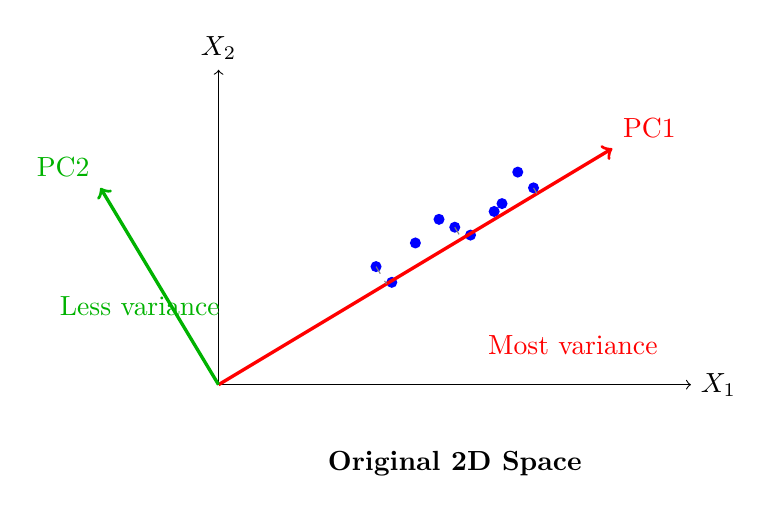
\begin{tikzpicture}[scale=1.0]
    % Original axes
    \draw[->] (0,0) -- (6,0) node[right] {$X_1$};
    \draw[->] (0,0) -- (0,4) node[above] {$X_2$};
    
    % Data points (elliptical cloud)
    \foreach \x/\y in {2/1.5, 2.5/1.8, 3/2, 3.5/2.2, 4/2.5, 2.2/1.3, 3.8/2.7, 3.2/1.9, 2.8/2.1, 3.6/2.3} {
        \fill[blue] (\x,\y) circle (2pt);
    }
    
    % PC1 (direction of maximum variance)
    \draw[->, very thick, red] (0,0) -- (5,3) node[above right] {PC1};
    
    % PC2 (orthogonal)
    \draw[->, very thick, green!70!black] (0,0) -- (-1.5,2.5) node[above left] {PC2};
    
    % Projections onto PC1
    \foreach \x/\y in {2/1.5, 3/2, 4/2.5} {
        \draw[dashed, gray] (\x,\y) -- ({(\x*5+\y*3)/(5^2+3^2)*5}, {(\x*5+\y*3)/(5^2+3^2)*3});
    }
    
    \node at (3, -1) {\textbf{Original 2D Space}};
    \node[red] at (4.5, 0.5) {Most variance};
    \node[green!70!black] at (-1, 1) {Less variance};
\end{tikzpicture}
\end{center}

\textbf{Key insight:} Data varies more along PC1 than PC2. Projecting onto PC1 alone captures most information!
\end{geometrybox}

\section{Complete Numerical Example}

\begin{example}[PCA by Hand]

\textbf{Data:} 5 samples, 2 features (already mean-centered)

\begin{center}
\begin{tabular}{|c|c|c|}
\hline
Sample & $X_1$ & $X_2$ \\
\hline
1 & -2 & -1 \\
2 & -1 & 0 \\
3 & 0 & 0 \\
4 & 1 & 1 \\
5 & 2 & 2 \\
\hline
\end{tabular}
\end{center}

\textbf{Data matrix (centered):}
\begin{equation}
    \mathbf{X} = \begin{bmatrix}
        -2 & -1 \\
        -1 & 0 \\
        0 & 0 \\
        1 & 1 \\
        2 & 2
    \end{bmatrix}
\end{equation}

\textbf{STEP 1: Compute covariance matrix}

\begin{align}
    \mathbf{C} &= \frac{1}{n-1}\mathbf{X}^T\mathbf{X} \\
    &= \frac{1}{4}\begin{bmatrix}
        -2 & -1 & 0 & 1 & 2 \\
        -1 & 0 & 0 & 1 & 2
    \end{bmatrix}\begin{bmatrix}
        -2 & -1 \\
        -1 & 0 \\
        0 & 0 \\
        1 & 1 \\
        2 & 2
    \end{bmatrix}
\end{align}

\textbf{Compute $\mathbf{X}^T\mathbf{X}$:}
\begin{align}
    \mathbf{X}^T\mathbf{X} &= \begin{bmatrix}
        4+1+0+1+4 & 2+0+0+1+4 \\
        2+0+0+1+4 & 1+0+0+1+4
    \end{bmatrix} \\
    &= \begin{bmatrix}
        10 & 7 \\
        7 & 6
    \end{bmatrix}
\end{align}

\begin{equation}
    \mathbf{C} = \frac{1}{4}\begin{bmatrix}
        10 & 7 \\
        7 & 6
    \end{bmatrix} = \begin{bmatrix}
        2.5 & 1.75 \\
        1.75 & 1.5
    \end{bmatrix}
\end{equation}

\textbf{STEP 2: Find eigenvalues}

\textbf{Characteristic equation:}
\begin{align}
    \det(\mathbf{C} - \lambda\mathbf{I}) &= \det\begin{bmatrix}
        2.5-\lambda & 1.75 \\
        1.75 & 1.5-\lambda
    \end{bmatrix} \\
    &= (2.5-\lambda)(1.5-\lambda) - (1.75)^2 \\
    &= 3.75 - 2.5\lambda - 1.5\lambda + \lambda^2 - 3.0625 \\
    &= \lambda^2 - 4\lambda + 0.6875 = 0
\end{align}

\textbf{Solve using quadratic formula:}
\begin{align}
    \lambda &= \frac{4 \pm \sqrt{16 - 2.75}}{2} = \frac{4 \pm \sqrt{13.25}}{2} = \frac{4 \pm 3.64}{2}
\end{align}

\begin{align}
    \lambda_1 &= \frac{4 + 3.64}{2} = 3.82 \\
    \lambda_2 &= \frac{4 - 3.64}{2} = 0.18
\end{align}

\textbf{STEP 3: Find eigenvectors}

\textbf{For $\lambda_1 = 3.82$:}
\begin{align}
    \begin{bmatrix}
        2.5-3.82 & 1.75 \\
        1.75 & 1.5-3.82
    \end{bmatrix}\begin{bmatrix} v_1 \\ v_2 \end{bmatrix} &= \begin{bmatrix} 0 \\ 0 \end{bmatrix} \\
    \begin{bmatrix}
        -1.32 & 1.75 \\
        1.75 & -2.32
    \end{bmatrix}\begin{bmatrix} v_1 \\ v_2 \end{bmatrix} &= \begin{bmatrix} 0 \\ 0 \end{bmatrix}
\end{align}

From first equation: $-1.32v_1 + 1.75v_2 = 0$

$\Rightarrow v_2 = \frac{1.32}{1.75}v_1 \approx 0.754v_1$

Let $v_1 = 1$, then $v_2 \approx 0.754$

\textbf{Eigenvector (unnormalized):} $\mathbf{v}_1 = \begin{bmatrix} 1 \\ 0.754 \end{bmatrix}$

\textbf{Normalize:}
\begin{align}
    ||\mathbf{v}_1|| &= \sqrt{1^2 + 0.754^2} = \sqrt{1.568} \approx 1.252 \\
    \mathbf{v}_1 &= \begin{bmatrix} 0.799 \\ 0.602 \end{bmatrix}
\end{align}

\textbf{For $\lambda_2 = 0.18$:}

Similarly (or use orthogonality):
\begin{equation}
    \mathbf{v}_2 = \begin{bmatrix} -0.602 \\ 0.799 \end{bmatrix}
\end{equation}

(Perpendicular to $\mathbf{v}_1$: $\mathbf{v}_1^T\mathbf{v}_2 = 0$)

\textbf{STEP 4: Variance explained}

\textbf{Total variance:}
\begin{equation}
    \text{Total} = \lambda_1 + \lambda_2 = 3.82 + 0.18 = 4.0
\end{equation}

\textbf{Variance explained by PC1:}
\begin{equation}
    \frac{\lambda_1}{\lambda_1 + \lambda_2} = \frac{3.82}{4.0} = 0.955 = 95.5\%
\end{equation}

\textbf{Variance explained by PC2:}
\begin{equation}
    \frac{\lambda_2}{\lambda_1 + \lambda_2} = \frac{0.18}{4.0} = 0.045 = 4.5\%
\end{equation}

\textbf{STEP 5: Project onto PC1 (reduce to 1D)}

\textbf{Projection matrix:}
\begin{equation}
    \mathbf{W} = \mathbf{v}_1 = \begin{bmatrix} 0.799 \\ 0.602 \end{bmatrix}
\end{equation}

\textbf{Transform data:}
\begin{align}
    \mathbf{Z} &= \mathbf{X}\mathbf{W} \\
    &= \begin{bmatrix}
        -2 & -1 \\
        -1 & 0 \\
        0 & 0 \\
        1 & 1 \\
        2 & 2
    \end{bmatrix}\begin{bmatrix} 0.799 \\ 0.602 \end{bmatrix} \\
    &= \begin{bmatrix}
        -2(0.799) + (-1)(0.602) \\
        -1(0.799) + 0(0.602) \\
        0(0.799) + 0(0.602) \\
        1(0.799) + 1(0.602) \\
        2(0.799) + 2(0.602)
    \end{bmatrix} \\
    &= \begin{bmatrix}
        -2.200 \\
        -0.799 \\
        0 \\
        1.401 \\
        2.802
    \end{bmatrix}
\end{align}

\textbf{Result:} Reduced from 2D to 1D, retaining 95.5\% of variance!
\end{example}

\section{Choosing Number of Components}

\begin{definition}[How Many PCs to Keep?]

\textbf{Method 1: Variance Explained Threshold}

Keep enough PCs to explain $\geq$ 80-95\% of total variance:

\begin{equation}
    \frac{\sum_{i=1}^{k}\lambda_i}{\sum_{i=1}^{p}\lambda_i} \geq 0.80
\end{equation}

\textbf{Method 2: Scree Plot}

Plot eigenvalues vs component number. Look for "elbow" where eigenvalues drop sharply.

\textbf{Method 3: Kaiser Criterion}

Keep components with $\lambda_i > 1$ (for standardized data).

Rationale: These explain more variance than a single original variable.

\textbf{Method 4: Cross-validation}

Use components as features in downstream task (e.g., classification).

Choose $k$ that gives best CV performance.

\textbf{Method 5: Domain knowledge}

Sometimes dimensionality is constrained by problem (e.g., 2D for visualization).
\end{definition}

\begin{geometrybox}
\textbf{Scree Plot:}

\begin{center}
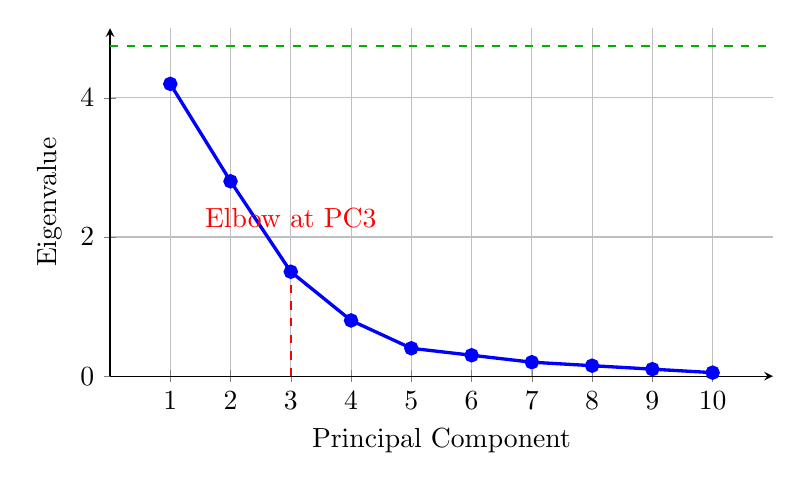
\begin{tikzpicture}[scale=1.0]
    \begin{axis}[
        axis lines = left,
        xlabel = {Principal Component},
        ylabel = {Eigenvalue},
        xmin=0, xmax=11,
        ymin=0, ymax=5,
        width=10cm,
        height=6cm,
        xtick={1,2,3,4,5,6,7,8,9,10},
        grid=major
    ]
    
    \addplot[blue, very thick, mark=*] coordinates {
        (1, 4.2) (2, 2.8) (3, 1.5) (4, 0.8) (5, 0.4) 
        (6, 0.3) (7, 0.2) (8, 0.15) (9, 0.1) (10, 0.05)
    };
    
    % Elbow
    \draw[red, thick, dashed] (3, 0) -- (3, 1.5);
    \node[red, above] at (3, 2) {Elbow at PC3};
    
    % Cumulative variance line
    \addplot[green!70!black, thick, dashed] coordinates {
        (0, 0.95*5) (11, 0.95*5)
    };
    \node[green!70!black, right] at (11, 0.95*5) {95\% threshold};
    
    \end{axis}
\end{tikzpicture}
\end{center}

\textbf{Interpretation:} Sharp drop after PC3 suggests keeping 3 components.
\end{geometrybox}

\section{PCA Properties and Insights}

\begin{theorem}[Key PCA Properties]

\textbf{1. Orthogonality:}

Principal components are mutually orthogonal (perpendicular):
\begin{equation}
    \mathbf{v}_i^T\mathbf{v}_j = 0 \quad \text{for } i \neq j
\end{equation}

\textbf{2. Uncorrelated:}

PC scores are uncorrelated:
\begin{equation}
    \text{Cov}(Z_i, Z_j) = 0 \quad \text{for } i \neq j
\end{equation}

\textbf{3. Maximum variance:}

Each PC captures maximum remaining variance subject to orthogonality.

\textbf{4. Reconstruction:}

Original data can be reconstructed (with error if $k < p$):
\begin{equation}
    \mathbf{X}_{\text{reconstructed}} = \mathbf{Z}\mathbf{W}^T
\end{equation}

\textbf{Reconstruction error:}
\begin{equation}
    \text{Error} = \sum_{i=k+1}^{p}\lambda_i
\end{equation}

(Sum of discarded eigenvalues)

\textbf{5. Scale invariance:}

PCA results depend on feature scales. \textbf{Always standardize!}

\textbf{6. Linear transformation:}

PCA finds best \textbf{linear} subspace. Can't capture non-linear structure.
\end{theorem}

\section{PCA vs Other Techniques}

\begin{importantbox}
\textbf{PCA vs LDA:}

\textbf{PCA (Unsupervised):}
\begin{itemize}
    \item Maximizes variance
    \item Ignores class labels
    \item For data exploration, visualization, preprocessing
\end{itemize}

\textbf{LDA (Supervised):}
\begin{itemize}
    \item Maximizes class separation
    \item Uses class labels
    \item For classification tasks
\end{itemize}

\textbf{Key difference:} PCA may not help classification! Highest variance directions might not separate classes.

\textbf{PCA vs Feature Selection:}

\textbf{PCA:}
\begin{itemize}
    \item Creates new features (linear combinations)
    \item Loses interpretability
    \item Uses all original features
\end{itemize}

\textbf{Feature Selection:}
\begin{itemize}
    \item Selects subset of original features
    \item Maintains interpretability
    \item Discards some features completely
\end{itemize}

\textbf{PCA vs Autoencoders:}

\textbf{PCA:}
\begin{itemize}
    \item Linear dimensionality reduction
    \item Fast, closed-form solution
    \item Optimal for linear structure
\end{itemize}

\textbf{Autoencoders:}
\begin{itemize}
    \item Non-linear dimensionality reduction
    \item Require training (slow)
    \item Can capture complex patterns
\end{itemize}
\end{importantbox}

\section{Applications of PCA}

\begin{definition}[Common Use Cases]

\textbf{1. Data Visualization:}
\begin{itemize}
    \item Reduce to 2D or 3D for plotting
    \item Explore high-dimensional data
    \item Identify clusters, outliers, patterns
\end{itemize}

\textbf{2. Noise Reduction:}
\begin{itemize}
    \item Keep only high-variance components
    \item Discard low-variance (noisy) components
    \item Reconstruct "denoised" data
\end{itemize}

\textbf{3. Feature Extraction:}
\begin{itemize}
    \item Create informative features for ML
    \item Reduce dimensionality before classification/regression
    \item Speed up training
\end{itemize}

\textbf{4. Compression:}
\begin{itemize}
    \item Store fewer dimensions
    \item Image compression (JPEG uses similar ideas)
    \item Reduce memory/storage requirements
\end{itemize}

\textbf{5. Multicollinearity Removal:}
\begin{itemize}
    \item PCs are uncorrelated by construction
    \item Improves stability of linear models
    \item Regularization effect
\end{itemize}

\textbf{6. Anomaly Detection:}
\begin{itemize}
    \item Points with large reconstruction error are outliers
    \item Project to PC space, measure distance
\end{itemize}
\end{definition}

\section{Limitations and Considerations}

\begin{keyidea}
\textbf{Advantages of PCA:}

\begin{enumerate}
    \item \textbf{Simple:} Easy to understand and implement
    \item \textbf{Fast:} Efficient computation (especially for small $p$)
    \item \textbf{Optimal:} Maximizes variance (for linear projection)
    \item \textbf{Uncorrelated features:} PCs are independent
    \item \textbf{Deterministic:} No random initialization
    \item \textbf{Noise reduction:} Filters out low-variance dimensions
    \item \textbf{Widely used:} Standard preprocessing step
\end{enumerate}

\textbf{Disadvantages of PCA:}

\begin{enumerate}
    \item \textbf{Linear:} Cannot capture non-linear structure
    \item \textbf{Scale-dependent:} Must standardize features
    \item \textbf{Interpretability loss:} PCs are linear combinations
    \item \textbf{Variance $\neq$ importance:} High variance doesn't mean informative for the task
    \item \textbf{Sensitive to outliers:} Covariance affected by extreme values
    \item \textbf{Unsupervised:} Ignores class labels (may hurt classification)
    \item \textbf{Assumes Gaussian:} Works best when data is normally distributed
    \item \textbf{Memory:} Needs to store covariance matrix ($p^2$)
\end{enumerate}
\end{keyidea}

\begin{importantbox}
\textbf{When NOT to use PCA:}

\begin{itemize}
    \item Features already uncorrelated
    \item Non-linear relationships dominate
    \item Need interpretable features
    \item Very small dataset (unstable estimates)
    \item Categorical/binary features (use other methods)
    \item Supervised task where variance doesn't indicate class separation
\end{itemize}

\textbf{Alternatives to consider:}
\begin{itemize}
    \item \textbf{t-SNE:} Non-linear, good for visualization
    \item \textbf{UMAP:} Non-linear, preserves global structure
    \item \textbf{Autoencoders:} Non-linear neural networks
    \item \textbf{Factor Analysis:} Assumes latent factors
    \item \textbf{ICA:} Independent (not just uncorrelated) components
\end{itemize}
\end{importantbox}

\section{Computational Complexity}

\begin{definition}[PCA Complexity]

For $n$ samples and $p$ features:

\textbf{Covariance matrix:} $O(np^2)$

\textbf{Eigendecomposition:} $O(p^3)$

\textbf{Projection:} $O(npk)$ where $k$ is reduced dimensions

\textbf{Total:} $O(np^2 + p^3)$

\textbf{Bottleneck:}
\begin{itemize}
    \item If $n > p$: Eigendecomposition dominates ($p^3$)
    \item If $n < p$: Covariance computation dominates ($np^2$)
\end{itemize}

\textbf{Optimization for large $p$:}

Use \textbf{Singular Value Decomposition (SVD)} instead:
\begin{itemize}
    \item Compute $\mathbf{X} = \mathbf{U}\boldsymbol{\Sigma}\mathbf{V}^T$
    \item Principal components are columns of $\mathbf{V}$
    \item Eigenvalues are $\sigma_i^2$
    \item More numerically stable
    \item Can use truncated SVD for large sparse matrices
\end{itemize}
\end{definition}

\section{GATE-Style Problems}

\begin{example}[Problem 1: Variance Explained]

\textbf{Given:} Dataset with 5 features

\textbf{Eigenvalues:} $\lambda = [5.2, 2.8, 1.5, 0.4, 0.1]$

\textbf{Questions:}
\begin{enumerate}
    \item What is total variance?
    \item What percentage of variance is explained by PC1?
    \item How many PCs needed to explain 90\% variance?
\end{enumerate}

\textbf{Solution:}

\textbf{1. Total variance:}
\begin{equation}
    \text{Total} = 5.2 + 2.8 + 1.5 + 0.4 + 0.1 = 10.0
\end{equation}

\textbf{2. Variance explained by PC1:}
\begin{equation}
    \frac{5.2}{10.0} = 0.52 = 52\%
\end{equation}

\textbf{3. Cumulative variance:}
\begin{align}
    \text{PC1:} & \quad 5.2/10.0 = 52\% \\
    \text{PC1+PC2:} & \quad (5.2+2.8)/10.0 = 80\% \\
    \text{PC1+PC2+PC3:} & \quad (5.2+2.8+1.5)/10.0 = 95\%
\end{align}

\textbf{Answer:} Need \textbf{3 PCs} to explain 90\% (actually explains 95\%)
\end{example}

\begin{example}[Problem 2: Computing PC Scores]

\textbf{Data point:} $\mathbf{x} = [4, 2]^T$ (centered)

\textbf{First principal component:} $\mathbf{v}_1 = [0.8, 0.6]^T$

\textbf{Compute the PC1 score.}

\textbf{Solution:}

\textbf{PC1 score:}
\begin{align}
    z_1 &= \mathbf{v}_1^T\mathbf{x} \\
    &= [0.8, 0.6]\begin{bmatrix} 4 \\ 2 \end{bmatrix} \\
    &= 0.8(4) + 0.6(2) \\
    &= 3.2 + 1.2 \\
    &= 4.4
\end{align}

\textbf{Answer:} PC1 score = 4.4
\end{example}

\begin{example}[Problem 3: Eigenvalue Interpretation]

\textbf{Question:} What does a larger eigenvalue indicate?

\textbf{Answer:}

A larger eigenvalue $\lambda_i$ indicates:
\begin{enumerate}
    \item \textbf{More variance} captured along that principal component
    \item \textbf{More important} direction in the data
    \item \textbf{More information} retained when projecting onto that PC
\end{enumerate}

\textbf{Quantitatively:}

If $\lambda_1 = 10$ and $\lambda_2 = 2$:
\begin{itemize}
    \item PC1 captures 5× more variance than PC2
    \item PC1 explains $10/12 = 83.3\%$ of total variance
    \item PC2 explains $2/12 = 16.7\%$ of total variance
\end{itemize}
\end{example}

\begin{example}[Problem 4: PCA vs LDA]

\textbf{Question:} You have 1000 images of handwritten digits (0-9). Which is better: PCA or LDA?

\textbf{Answer:}

\textbf{LDA is better} for this task because:

\textbf{Reason:}
\begin{itemize}
    \item This is a \textbf{supervised} classification task
    \item We have class labels (digits 0-9)
    \item LDA maximizes \textbf{class separation}
    \item PCA only maximizes variance (may not separate classes)
\end{itemize}

\textbf{Example scenario:}
\begin{itemize}
    \item PCA might find PC1 = "overall brightness" (high variance)
    \item But brightness might not help distinguish 3 vs 8!
    \item LDA finds directions that best separate different digits
\end{itemize}

\textbf{When PCA could help:}
\begin{itemize}
    \item As preprocessing before LDA (reduce 1000 pixels to 100)
    \item For data exploration/visualization
    \item To remove noise before classification
\end{itemize}
\end{example}

\section{Summary - Key Points for GATE}

\begin{importantbox}
\textbf{Must Know for GATE:}

\begin{enumerate}
    \item \textbf{Goal:} Reduce dimensionality while preserving variance
    
    \item \textbf{Mathematical foundation:}
    \begin{itemize}
        \item Principal components = eigenvectors of covariance matrix
        \item Eigenvalues = variance along each PC
        \item Eigenvector equation: $\mathbf{C}\mathbf{v} = \lambda\mathbf{v}$
    \end{itemize}
    
    \item \textbf{Algorithm steps:}
    \begin{enumerate}
        \item Standardize data (center and scale)
        \item Compute covariance matrix: $\mathbf{C} = \frac{1}{n-1}\mathbf{X}^T\mathbf{X}$
        \item Find eigenvalues and eigenvectors
        \item Sort by eigenvalue (descending)
        \item Select top $k$ eigenvectors
        \item Project: $\mathbf{Z} = \mathbf{X}\mathbf{W}$
    \end{enumerate}
    
    \item \textbf{Variance explained:}
    \begin{equation}
        \text{Explained by PC}_i = \frac{\lambda_i}{\sum_j \lambda_j}
    \end{equation}
    
    \item \textbf{Choosing $k$:}
    \begin{itemize}
        \item Variance threshold (80-95\%)
        \item Scree plot elbow
        \item Kaiser criterion ($\lambda > 1$)
        \item Cross-validation
    \end{itemize}
    
    \item \textbf{Properties:}
    \begin{itemize}
        \item PCs are orthogonal (perpendicular)
        \item PC scores are uncorrelated
        \item PC1 has maximum variance
        \item Each PC captures maximum remaining variance
    \end{itemize}
    
    \item \textbf{Advantages:}
    \begin{itemize}
        \item Simple, fast, deterministic
        \item Removes multicollinearity
        \item Reduces noise
        \item Optimal linear projection
    \end{itemize}
    
    \item \textbf{Disadvantages:}
    \begin{itemize}
        \item Linear only
        \item Scale-dependent (must standardize)
        \item Loses interpretability
        \item Unsupervised (ignores labels)
        \item Sensitive to outliers
    \end{itemize}
    
    \item \textbf{PCA vs LDA:}
    \begin{itemize}
        \item PCA: Unsupervised, maximizes variance
        \item LDA: Supervised, maximizes class separation
    \end{itemize}
    
    \item \textbf{Computational complexity:}
    \begin{itemize}
        \item Covariance: $O(np^2)$
        \item Eigendecomposition: $O(p^3)$
        \item Total: $O(np^2 + p^3)$
    \end{itemize}
    
    \item \textbf{Applications:}
    \begin{itemize}
        \item Visualization (reduce to 2D/3D)
        \item Noise reduction
        \item Feature extraction
        \item Compression
        \item Preprocessing for ML
    \end{itemize}
    
    \item \textbf{Important formulas:}
    \begin{align}
        \mathbf{C} &= \frac{1}{n-1}\mathbf{X}^T\mathbf{X} \\
        \mathbf{C}\mathbf{v} &= \lambda\mathbf{v} \\
        \mathbf{Z} &= \mathbf{X}\mathbf{W} \\
        \text{Reconstruction:} & \quad \mathbf{X} \approx \mathbf{Z}\mathbf{W}^T
    \end{align}
\end{enumerate}
\end{importantbox}

\begin{gatepoint}
\textbf{Common GATE Question Types:}

\begin{enumerate}
    \item Calculate covariance matrix from data
    \item Compute eigenvalues and eigenvectors
    \item Calculate variance explained by each PC
    \item Determine number of PCs needed for threshold
    \item Project data onto principal components
    \item Interpret eigenvalues/eigenvectors
    \item Understand geometric interpretation
    \item Compare PCA with LDA
    \item Know when to use/not use PCA
    \item Understand orthogonality of PCs
    \item Calculate reconstruction error
    \item Know computational complexity
    \item Understand effect of standardization
\end{enumerate}
\end{gatepoint}
\end{document}